\documentclass[twoside]{book}

% Packages required by doxygen
\usepackage{fixltx2e}
\usepackage{calc}
\usepackage{doxygen}
\usepackage[export]{adjustbox} % also loads graphicx
\usepackage{graphicx}
\usepackage[utf8]{inputenc}
\usepackage{makeidx}
\usepackage{multicol}
\usepackage{multirow}
\PassOptionsToPackage{warn}{textcomp}
\usepackage{textcomp}
\usepackage[nointegrals]{wasysym}
\usepackage[table]{xcolor}

% Font selection
\usepackage[T1]{fontenc}
\usepackage[scaled=.90]{helvet}
\usepackage{courier}
\usepackage{amssymb}
\usepackage{sectsty}
\renewcommand{\familydefault}{\sfdefault}
\allsectionsfont{%
  \fontseries{bc}\selectfont%
  \color{darkgray}%
}
\renewcommand{\DoxyLabelFont}{%
  \fontseries{bc}\selectfont%
  \color{darkgray}%
}
\newcommand{\+}{\discretionary{\mbox{\scriptsize$\hookleftarrow$}}{}{}}

% Page & text layout
\usepackage{geometry}
\geometry{%
  a4paper,%
  top=2.5cm,%
  bottom=2.5cm,%
  left=2.5cm,%
  right=2.5cm%
}
\tolerance=750
\hfuzz=15pt
\hbadness=750
\setlength{\emergencystretch}{15pt}
\setlength{\parindent}{0cm}
\setlength{\parskip}{0.2cm}
\makeatletter
\renewcommand{\paragraph}{%
  \@startsection{paragraph}{4}{0ex}{-1.0ex}{1.0ex}{%
    \normalfont\normalsize\bfseries\SS@parafont%
  }%
}
\renewcommand{\subparagraph}{%
  \@startsection{subparagraph}{5}{0ex}{-1.0ex}{1.0ex}{%
    \normalfont\normalsize\bfseries\SS@subparafont%
  }%
}
\makeatother

% Headers & footers
\usepackage{fancyhdr}
\pagestyle{fancyplain}
\fancyhead[LE]{\fancyplain{}{\bfseries\thepage}}
\fancyhead[CE]{\fancyplain{}{}}
\fancyhead[RE]{\fancyplain{}{\bfseries\leftmark}}
\fancyhead[LO]{\fancyplain{}{\bfseries\rightmark}}
\fancyhead[CO]{\fancyplain{}{}}
\fancyhead[RO]{\fancyplain{}{\bfseries\thepage}}
\fancyfoot[LE]{\fancyplain{}{}}
\fancyfoot[CE]{\fancyplain{}{}}
\fancyfoot[RE]{\fancyplain{}{\bfseries\scriptsize Generated on Thu Oct 22 2015 18\+:50\+:14 for Civil\+Octave by Doxygen }}
\fancyfoot[LO]{\fancyplain{}{\bfseries\scriptsize Generated on Thu Oct 22 2015 18\+:50\+:14 for Civil\+Octave by Doxygen }}
\fancyfoot[CO]{\fancyplain{}{}}
\fancyfoot[RO]{\fancyplain{}{}}
\renewcommand{\footrulewidth}{0.4pt}
\renewcommand{\chaptermark}[1]{%
  \markboth{#1}{}%
}
\renewcommand{\sectionmark}[1]{%
  \markright{\thesection\ #1}%
}

% Indices & bibliography
\usepackage{natbib}
\usepackage[titles]{tocloft}
\setcounter{tocdepth}{3}
\setcounter{secnumdepth}{5}
\makeindex

% Hyperlinks (required, but should be loaded last)
\usepackage{ifpdf}
\ifpdf
  \usepackage[pdftex,pagebackref=true]{hyperref}
\else
  \usepackage[ps2pdf,pagebackref=true]{hyperref}
\fi
\hypersetup{%
  colorlinks=true,%
  linkcolor=blue,%
  citecolor=blue,%
  unicode%
}

% Custom commands
\newcommand{\clearemptydoublepage}{%
  \newpage{\pagestyle{empty}\cleardoublepage}%
}


%===== C O N T E N T S =====

\begin{document}

% Titlepage & ToC
\hypersetup{pageanchor=false,
             bookmarks=true,
             bookmarksnumbered=true,
             pdfencoding=unicode
            }
\pagenumbering{roman}
\begin{titlepage}
\vspace*{7cm}
\begin{center}%
{\Large Civil\+Octave }\\
\vspace*{1cm}
{\large Generated by Doxygen 1.8.11}\\
\vspace*{0.5cm}
{\small Thu Oct 22 2015 18:50:14}\\
\end{center}
\end{titlepage}
\clearemptydoublepage
\tableofcontents
\clearemptydoublepage
\pagenumbering{arabic}
\hypersetup{pageanchor=true}

%--- Begin generated contents ---
\chapter{Main Page}
\label{index}\hypertarget{index}{}Use of Octave (Mat\+L\+A\+B) in Civil Engineering Problems

To run this program, you need to install {\ttfamily G\+N\+U octave} on your computer. To know how to obtain it, visit\+: \href{https://www.gnu.org/software/octave/}{\tt https\+://www.\+gnu.\+org/software/octave/}

Once you have G\+N\+U Octave working, go to folder where code for an example is present. For example to run code correspond to example L01, go to folder Example/\+L01, ( for example on G\+N\+U/\+Linux you may do so by\+: {\ttfamily cd Example/\+L01} ). The code is in file {\ttfamily main.\+m}, and data is in file {\ttfamily input.\+mat}. To store results in file {\ttfamily output.\+txt}, type command\+:

{\ttfamily octave main.\+m $>$ output.\+txt}

or in following form, if we wish to produce pdf using La\+Te\+X from folder (tex, if available) using \hyperlink{run_8sh}{run.\+sh}

{\ttfamily octave main.\+m $>$ output.\+tex}

View file output.\+txt in any text editor, or main.\+pdf (in tex folder) in pdf viewer.

Authors acknowledge used of function written by Sachin Shanbhag.

\href{http://sachinashanbhag.blogspot.in/2012/11/exporting-matrices-in-octavematlab-to.html}{\tt http\+://sachinashanbhag.\+blogspot.\+in/2012/11/exporting-\/matrices-\/in-\/octavematlab-\/to.\+html}

\href{https://docs.google.com/open?id=0Bww3OZktvGQucmxnd1FJNElCVGc}{\tt https\+://docs.\+google.\+com/open?id=0\+Bww3\+O\+Zktv\+G\+Qucmxnd1\+F\+J\+N\+El\+C\+V\+Gc}

\#\+Sage Use of Sage in Civil Engineering Problems

Requirement-\/\+:

\subsection*{1. Sagemath}

\subsection*{2. latex}

\subsection*{3. Django}
\chapter{Contribute}
\label{a00002}
\hypertarget{a00002}{}
\#\+Contribute

If you want to contribute to this project, then just fork this repository.


\begin{DoxyItemize}
\item Run this command to not sharing your \hyperlink{a00022}{settings.\+py} file while sending Pull Request\+:
\end{DoxyItemize}

{\ttfamily git update-\/index -\/-\/assume-\/unchanged \hyperlink{a00022}{sage/sage/settings.\+py}}


\begin{DoxyItemize}
\item Modify the code. Find Bugs. Solve Bugs.
\item Commit. Push. Send P\+R.
\end{DoxyItemize}

\+:) 
\chapter{S\+A\+G\+E}
\label{a00004}
\hypertarget{a00004}{}
\subsection*{I\+N\+S\+A\+T\+L\+L\+A\+T\+I\+O\+N -\/\+:}


\begin{DoxyEnumerate}
\item Just clone or fork from
\item Go to terminal and go to cd /path/to/folder/\+Civil\+Octave/sage
\item Run command python \hyperlink{a00020}{manage.\+py} migrate
\item Run app using python \hyperlink{a00020}{manage.\+py} runserver
\end{DoxyEnumerate}

\subsubsection*{F\+O\+L\+D\+E\+R\+S -\/\+:}


\begin{DoxyEnumerate}
\item civilsage -\/ contain Django code for interface
\item sagemath -\/ contain Sagemath and La\+Te\+X code
\item sage -\/ contain Django setting.\+py 
\end{DoxyEnumerate}
\chapter{Namespace Index}
\section{Packages}
Here are the packages with brief descriptions (if available)\+:\begin{DoxyCompactList}
\item\contentsline{section}{\hyperlink{namespacecivilsage}{civilsage} }{\pageref{namespacecivilsage}}{}
\item\contentsline{section}{\hyperlink{namespacecivilsage_1_1admin}{civilsage.\+admin} }{\pageref{namespacecivilsage_1_1admin}}{}
\item\contentsline{section}{\hyperlink{namespacecivilsage_1_1models}{civilsage.\+models} }{\pageref{namespacecivilsage_1_1models}}{}
\item\contentsline{section}{\hyperlink{namespacecivilsage_1_1tests}{civilsage.\+tests} }{\pageref{namespacecivilsage_1_1tests}}{}
\item\contentsline{section}{\hyperlink{namespacecivilsage_1_1urls}{civilsage.\+urls} \\*This module contain urlspatterns to map to html file in django }{\pageref{namespacecivilsage_1_1urls}}{}
\item\contentsline{section}{\hyperlink{namespacecivilsage_1_1views}{civilsage.\+views} \\*This module contain functions to controls veiws of django }{\pageref{namespacecivilsage_1_1views}}{}
\item\contentsline{section}{\hyperlink{namespaceinitial__file}{initial\+\_\+file} \\*This module contain functions for processing the intruppted files }{\pageref{namespaceinitial__file}}{}
\item\contentsline{section}{\hyperlink{namespaceinput}{input} }{\pageref{namespaceinput}}{}
\item\contentsline{section}{\hyperlink{namespacemain}{main} }{\pageref{namespacemain}}{}
\item\contentsline{section}{\hyperlink{namespacemanage}{manage} \\*This code to start server and application additional argument is find initial to start processing of intruppted files }{\pageref{namespacemanage}}{}
\item\contentsline{section}{\hyperlink{namespacesage}{sage} }{\pageref{namespacesage}}{}
\item\contentsline{section}{\hyperlink{namespacesage_1_1settings}{sage.\+settings} \\*Django settings for sage project }{\pageref{namespacesage_1_1settings}}{}
\item\contentsline{section}{\hyperlink{namespacesage_1_1urls}{sage.\+urls} \\*This module contain urlspatterns to map to \hyperlink{namespacecivilsage_1_1urls}{civilsage.\+urls} in django }{\pageref{namespacesage_1_1urls}}{}
\item\contentsline{section}{\hyperlink{namespacesage_1_1wsgi}{sage.\+wsgi} }{\pageref{namespacesage_1_1wsgi}}{}
\item\contentsline{section}{\hyperlink{namespacesagemath}{sagemath} }{\pageref{namespacesagemath}}{}
\item\contentsline{section}{\hyperlink{namespacesagemath_1_1input}{sagemath.\+input} \\*This file contain input for \hyperlink{main_8sage}{main.\+sage} }{\pageref{namespacesagemath_1_1input}}{}
\item\contentsline{section}{\hyperlink{namespacesagemath_1_1main}{sagemath.\+main} \\*This module contain code to process the data obtain from \hyperlink{input_8sage}{input.\+sage} }{\pageref{namespacesagemath_1_1main}}{}
\end{DoxyCompactList}

\chapter{File Index}
\section{File List}
Here is a list of all files with brief descriptions\+:\begin{DoxyCompactList}
\item\contentsline{section}{/home/amarjeet/projects/\+Civil\+Octave/\+Examples/\+Do\+S/01/\hyperlink{DoS_201_2main_8m}{main.\+m} }{\pageref{DoS_201_2main_8m}}{}
\item\contentsline{section}{/home/amarjeet/projects/\+Civil\+Octave/\+Examples/\+Do\+S/01/tex/\hyperlink{abstract_8tex}{abstract.\+tex} }{\pageref{abstract_8tex}}{}
\item\contentsline{section}{/home/amarjeet/projects/\+Civil\+Octave/\+Examples/\+Do\+S/01/tex/\hyperlink{main_8tex}{main.\+tex} }{\pageref{main_8tex}}{}
\item\contentsline{section}{/home/amarjeet/projects/\+Civil\+Octave/\+Examples/\+Do\+S/01/tex/\hyperlink{run_8sh}{run.\+sh} }{\pageref{run_8sh}}{}
\item\contentsline{section}{/home/amarjeet/projects/\+Civil\+Octave/\+Examples/\+Do\+S/01/tex/\hyperlink{title_8tex}{title.\+tex} }{\pageref{title_8tex}}{}
\item\contentsline{section}{/home/amarjeet/projects/\+Civil\+Octave/\+Examples/\+Do\+S/01/tex/\hyperlink{usepackage_8tex}{usepackage.\+tex} }{\pageref{usepackage_8tex}}{}
\item\contentsline{section}{/home/amarjeet/projects/\+Civil\+Octave/\+Examples/\+Geo\+Tech/\+B\+C/\hyperlink{GeoTech_2BC_2main_8m}{main.\+m} }{\pageref{GeoTech_2BC_2main_8m}}{}
\item\contentsline{section}{/home/amarjeet/projects/\+Civil\+Octave/\+Examples/\+L01/\hyperlink{L01_2main_8m}{main.\+m} }{\pageref{L01_2main_8m}}{}
\item\contentsline{section}{/home/amarjeet/projects/\+Civil\+Octave/\+Examples/\+L02/\hyperlink{L02_2main_8m}{main.\+m} }{\pageref{L02_2main_8m}}{}
\item\contentsline{section}{/home/amarjeet/projects/\+Civil\+Octave/sage/\hyperlink{civil_8sh}{civil.\+sh} }{\pageref{civil_8sh}}{}
\item\contentsline{section}{/home/amarjeet/projects/\+Civil\+Octave/sage/\hyperlink{initial__file_8py}{initial\+\_\+file.\+py} }{\pageref{initial__file_8py}}{}
\item\contentsline{section}{/home/amarjeet/projects/\+Civil\+Octave/sage/\hyperlink{manage_8py}{manage.\+py} }{\pageref{manage_8py}}{}
\item\contentsline{section}{/home/amarjeet/projects/\+Civil\+Octave/sage/civilsage/\hyperlink{civilsage_2____init_____8py}{\+\_\+\+\_\+init\+\_\+\+\_\+.\+py} }{\pageref{civilsage_2____init_____8py}}{}
\item\contentsline{section}{/home/amarjeet/projects/\+Civil\+Octave/sage/civilsage/\hyperlink{admin_8py}{admin.\+py} }{\pageref{admin_8py}}{}
\item\contentsline{section}{/home/amarjeet/projects/\+Civil\+Octave/sage/civilsage/\hyperlink{models_8py}{models.\+py} }{\pageref{models_8py}}{}
\item\contentsline{section}{/home/amarjeet/projects/\+Civil\+Octave/sage/civilsage/\hyperlink{tests_8py}{tests.\+py} }{\pageref{tests_8py}}{}
\item\contentsline{section}{/home/amarjeet/projects/\+Civil\+Octave/sage/civilsage/\hyperlink{civilsage_2urls_8py}{urls.\+py} }{\pageref{civilsage_2urls_8py}}{}
\item\contentsline{section}{/home/amarjeet/projects/\+Civil\+Octave/sage/civilsage/\hyperlink{views_8py}{views.\+py} }{\pageref{views_8py}}{}
\item\contentsline{section}{/home/amarjeet/projects/\+Civil\+Octave/sage/civilsage/templates/\hyperlink{base_8html}{base.\+html} }{\pageref{base_8html}}{}
\item\contentsline{section}{/home/amarjeet/projects/\+Civil\+Octave/sage/civilsage/templates/civilsage/\hyperlink{file_8html}{file.\+html} }{\pageref{file_8html}}{}
\item\contentsline{section}{/home/amarjeet/projects/\+Civil\+Octave/sage/civilsage/templates/civilsage/\hyperlink{index_8html}{index.\+html} }{\pageref{index_8html}}{}
\item\contentsline{section}{/home/amarjeet/projects/\+Civil\+Octave/sage/civilsage/templates/civilsage/\hyperlink{matrix_8html}{matrix.\+html} }{\pageref{matrix_8html}}{}
\item\contentsline{section}{/home/amarjeet/projects/\+Civil\+Octave/sage/sage/\hyperlink{sage_2____init_____8py}{\+\_\+\+\_\+init\+\_\+\+\_\+.\+py} }{\pageref{sage_2____init_____8py}}{}
\item\contentsline{section}{/home/amarjeet/projects/\+Civil\+Octave/sage/sage/\hyperlink{settings_8py}{settings.\+py} }{\pageref{settings_8py}}{}
\item\contentsline{section}{/home/amarjeet/projects/\+Civil\+Octave/sage/sage/\hyperlink{sage_2urls_8py}{urls.\+py} }{\pageref{sage_2urls_8py}}{}
\item\contentsline{section}{/home/amarjeet/projects/\+Civil\+Octave/sage/sage/\hyperlink{wsgi_8py}{wsgi.\+py} }{\pageref{wsgi_8py}}{}
\item\contentsline{section}{/home/amarjeet/projects/\+Civil\+Octave/sage/sagemath/\hyperlink{civil_8tex}{civil.\+tex} }{\pageref{civil_8tex}}{}
\item\contentsline{section}{/home/amarjeet/projects/\+Civil\+Octave/sage/sagemath/\hyperlink{input_8sage}{input.\+sage} }{\pageref{input_8sage}}{}
\item\contentsline{section}{/home/amarjeet/projects/\+Civil\+Octave/sage/sagemath/\hyperlink{input_8sage_8py}{input.\+sage.\+py} }{\pageref{input_8sage_8py}}{}
\item\contentsline{section}{/home/amarjeet/projects/\+Civil\+Octave/sage/sagemath/\hyperlink{main_8sage}{main.\+sage} }{\pageref{main_8sage}}{}
\item\contentsline{section}{/home/amarjeet/projects/\+Civil\+Octave/sage/sagemath/\hyperlink{main_8sage_8py}{main.\+sage.\+py} }{\pageref{main_8sage_8py}}{}
\item\contentsline{section}{/home/amarjeet/projects/\+Civil\+Octave/sage/static/js/\hyperlink{autofill_8js}{autofill.\+js} }{\pageref{autofill_8js}}{}
\item\contentsline{section}{/home/amarjeet/projects/\+Civil\+Octave/sage/static/js/\hyperlink{bootstrap_8min_8js}{bootstrap.\+min.\+js} }{\pageref{bootstrap_8min_8js}}{}
\item\contentsline{section}{/home/amarjeet/projects/\+Civil\+Octave/sage/static/js/\hyperlink{jquery_8min_8js}{jquery.\+min.\+js} }{\pageref{jquery_8min_8js}}{}
\end{DoxyCompactList}

\chapter{Namespace Documentation}
\hypertarget{a00031}{}\section{civilsage Namespace Reference}
\label{a00031}\index{civilsage@{civilsage}}
\subsection*{Namespaces}
\begin{DoxyCompactItemize}
\item 
 \hyperlink{a00032}{admin}
\item 
 \hyperlink{a00033}{models}
\item 
 \hyperlink{a00034}{tests}
\item 
 \hyperlink{a00035}{urls}
\item 
 \hyperlink{a00036}{views}
\end{DoxyCompactItemize}

\hypertarget{a00032}{}\section{civilsage.\+admin Namespace Reference}
\label{a00032}\index{civilsage.\+admin@{civilsage.\+admin}}

\hypertarget{a00033}{}\section{civilsage.\+models Namespace Reference}
\label{a00033}\index{civilsage.\+models@{civilsage.\+models}}

\hypertarget{a00034}{}\section{civilsage.\+tests Namespace Reference}
\label{a00034}\index{civilsage.\+tests@{civilsage.\+tests}}

\hypertarget{a00035}{}\section{civilsage.\+urls Namespace Reference}
\label{a00035}\index{civilsage.\+urls@{civilsage.\+urls}}
\subsection*{Variables}
\begin{DoxyCompactItemize}
\item 
list \hyperlink{a00035_a46a501661622e9e2b11c9d6da43bbec0}{urlpatterns}
\end{DoxyCompactItemize}


\subsection{Variable Documentation}
\hypertarget{a00035_a46a501661622e9e2b11c9d6da43bbec0}{}\index{civilsage\+::urls@{civilsage\+::urls}!urlpatterns@{urlpatterns}}
\index{urlpatterns@{urlpatterns}!civilsage\+::urls@{civilsage\+::urls}}
\subsubsection[{urlpatterns}]{\setlength{\rightskip}{0pt plus 5cm}list civilsage.\+urls.\+urlpatterns}\label{a00035_a46a501661622e9e2b11c9d6da43bbec0}
{\bfseries Initial value\+:}
\begin{DoxyCode}
1 = [
2     \textcolor{comment}{#directs to index veiw}
3     url(\textcolor{stringliteral}{r'^$'}, views.index, name=\textcolor{stringliteral}{'index'}),
4     \textcolor{comment}{#directs request to matrix veiw}
5     url(\textcolor{stringliteral}{r'^matrix/$'}, views.matrix, name=\textcolor{stringliteral}{'matrix'}),
6     \textcolor{comment}{#directs request to file veiw to upload file}
7     url(\textcolor{stringliteral}{r'^file/$'}, views.file, name=\textcolor{stringliteral}{'file'}),
8     \textcolor{comment}{#directs request to last veiw}
9     url(\textcolor{stringliteral}{r'^last/$'}, views.last, name=\textcolor{stringliteral}{'last'}),
10 ]
\end{DoxyCode}


Definition at line 5 of file urls.\+py.


\hypertarget{a00036}{}\section{civilsage.\+views Namespace Reference}
\label{a00036}\index{civilsage.\+views@{civilsage.\+views}}
\subsection*{Functions}
\begin{DoxyCompactItemize}
\item 
def \hyperlink{a00036_a32de127956738677913352a2db84ecdb}{file} (request)
\item 
def \hyperlink{a00036_ad9397359f36a9df37e0aa43f3be032a3}{first\+\_\+write} (request)
\item 
def \hyperlink{a00036_a7b4fd4478a312ce8e35a192159c59de9}{index} (request)
\item 
def \hyperlink{a00036_aed47fb0740a2fa14693f697905788719}{last} (request)
\item 
def \hyperlink{a00036_a8b58c93a9c82e84143c43dafaa744a4b}{matrix} (request)
\item 
def \hyperlink{a00036_a9914ff19f8e15ccab1a07eaeac8cfb21}{pdfemail} (request, name)
\end{DoxyCompactItemize}


\subsection{Detailed Description}
\begin{DoxyVerb}@package docstring
This module contain functions to controls veiws
...
\end{DoxyVerb}
 

\subsection{Function Documentation}
\hypertarget{a00036_a32de127956738677913352a2db84ecdb}{}\index{civilsage\+::views@{civilsage\+::views}!file@{file}}
\index{file@{file}!civilsage\+::views@{civilsage\+::views}}
\subsubsection[{file(request)}]{\setlength{\rightskip}{0pt plus 5cm}def civilsage.\+views.\+file (
\begin{DoxyParamCaption}
\item[{}]{request}
\end{DoxyParamCaption}
)}\label{a00036_a32de127956738677913352a2db84ecdb}
\begin{DoxyVerb}Documentation for a function
This veiw take input data from file uploaded by user and processes
to give output in form of response
\end{DoxyVerb}
 

Definition at line 153 of file views.\+py.


\begin{DoxyCode}
153 \textcolor{keyword}{def }\hyperlink{a00036_a32de127956738677913352a2db84ecdb}{file}(request):
154 
155     \textcolor{stringliteral}{"""Documentation for a function}
156 \textcolor{stringliteral}{    This veiw take input data from file uploaded by user and processes}
157 \textcolor{stringliteral}{    to give output in form of response}
158 \textcolor{stringliteral}{    """}
159 
160     message=\textcolor{stringliteral}{'please fill again'}
161     \textcolor{keywordflow}{try}:
162         name,message=\hyperlink{a00036_ad9397359f36a9df37e0aa43f3be032a3}{first\_write}(request)
163         \textcolor{comment}{#getting file uploaded by user}
164         f=request.FILES[\textcolor{stringliteral}{"input\_file"}]
165         \hyperlink{a00029_ac2d69f5011896c6ed4a54e0dd36f6334}{if}(f.content\_type != \textcolor{stringliteral}{'text/csv'}):
166             \textcolor{keywordflow}{return} render( request,\textcolor{stringliteral}{'civilsage/file.html'},
167             \{\textcolor{stringliteral}{'email\_get'}: request.session.get(\textcolor{stringliteral}{'email\_get'}),
168             \textcolor{stringliteral}{'message'}:\textcolor{stringliteral}{'File Not in CSV FORMAT '}\})
169         data = [row \textcolor{keywordflow}{for} row \textcolor{keywordflow}{in} csv.reader(f)]
170         \textcolor{comment}{#getting numbers of storeys}
171         num = request.session.get(\textcolor{stringliteral}{'Number\_of\_storeys'})
172 
173         \textcolor{comment}{#opening input.sage to append remaining inputs}
174         command=name+\textcolor{stringliteral}{'/input.sage'}
175         file=open(command,\textcolor{stringliteral}{'a'})
176         \textcolor{comment}{#list of basic tags}
177         var = [\textcolor{stringliteral}{'mass'},\textcolor{stringliteral}{'Height\_storey'},\textcolor{stringliteral}{'Stiffness\_storey'}]
178         jar=0
179 
180         \textcolor{comment}{#writing matix into sage file}
181         \textcolor{keywordflow}{for} j \textcolor{keywordflow}{in} var:
182             message=\textcolor{stringliteral}{"Less no. of rows in csv file"}
183             file.write(j)
184             file.write(\textcolor{stringliteral}{'=matrix(['})
185 
186             \textcolor{comment}{#writing elements of matix}
187             \textcolor{keywordflow}{for} i \textcolor{keywordflow}{in} range(int(num)):
188                 file.write(\textcolor{stringliteral}{'['})
189 
190                 \textcolor{comment}{#getting input from tags}
191                 message=\textcolor{stringliteral}{"Less no. of elements in row "}+str(i)
192                 \hyperlink{a00029_ac2d69f5011896c6ed4a54e0dd36f6334}{if}(\textcolor{keywordflow}{not} data[jar][i].isdigit()):
193                     ii=i+1
194                 \textcolor{keywordflow}{else}:
195                     ii=i
196                 d=data[jar][ii]
197                 file.write(str(d))
198                 file.write(\textcolor{stringliteral}{']'})
199 
200                 \textcolor{comment}{#condition to check last element}
201                 \hyperlink{a00029_ac2d69f5011896c6ed4a54e0dd36f6334}{if}( i!=int(num)+jar-1):
202                     file.write(\textcolor{stringliteral}{','})
203             jar=jar+1
204             file.write(\textcolor{stringliteral}{'])\(\backslash\)n'})
205         file.close()
206         \hyperlink{a00029_ac2d69f5011896c6ed4a54e0dd36f6334}{if}(request.POST.get(\textcolor{stringliteral}{'email\_id'})):
207             \textcolor{comment}{#calling funcion to send pdf and run that as background proces}
208             thread = threading.Thread(target=pdfemail,args=(request,name))
209             thread.daemon = \textcolor{keyword}{True}
210             thread.start()
211             message=\textcolor{stringliteral}{"PDF send to "}+request.POST.get(\textcolor{stringliteral}{'email\_id'})
212             \textcolor{keywordflow}{return} render(request, \textcolor{stringliteral}{"civilsage/index.html"}, \{\textcolor{stringliteral}{'message'}:message\})
213         \textcolor{keywordflow}{else}:
214             \textcolor{comment}{#creating and writing sh file for background processing}
215             command=name+\textcolor{stringliteral}{'/civil.sh'}
216             file=open(command,\textcolor{stringliteral}{'w'})
217             command=\textcolor{stringliteral}{'cd '}+name
218             file.write(command)
219             file.write(\textcolor{stringliteral}{'\(\backslash\)nlatex civil.tex\(\backslash\)nsage civil.sagetex.sage\(\backslash\)n'})
220             file.write(\textcolor{stringliteral}{'pdflatex civil.tex\(\backslash\)n'})
221             file.close()
222 
223             \textcolor{comment}{#calling sh file for background processing}
224             command=\textcolor{stringliteral}{'sh '}+name+\textcolor{stringliteral}{'/civil.sh'}
225             os.system(command)
226 
227             \textcolor{comment}{#opening creted pdf to display to user}
228             command=name+\textcolor{stringliteral}{'/civil.pdf'}
229             f=open(command)
230 
231             \textcolor{comment}{#sending pdf as response}
232             response = HttpResponse(f,content\_type=\textcolor{stringliteral}{'application/pdf'})
233             response[\textcolor{stringliteral}{'Content-Disposition'}] = \textcolor{stringliteral}{'attachment; filename="civil.pdf"'}
234             \textcolor{comment}{#deleting temperary files}
235             command=\textcolor{stringliteral}{'rm -rf '}+name
236             os.system(command)
237             \textcolor{keywordflow}{return} response
238     \textcolor{keywordflow}{except}:
239         \textcolor{keywordflow}{return} render(request, \textcolor{stringliteral}{"civilsage/file.html"},
240         \{\textcolor{stringliteral}{'message'}:message,\textcolor{stringliteral}{'email\_get'}:request.session.get(\textcolor{stringliteral}{'email\_get'})\})
241 
\end{DoxyCode}


Here is the call graph for this function\+:\nopagebreak
\begin{figure}[H]
\begin{center}
\leavevmode

\includegraphics[width=320pt]{a00036_a32de127956738677913352a2db84ecdb_cgraph}
\end{center}
\end{figure}


\hypertarget{a00036_ad9397359f36a9df37e0aa43f3be032a3}{}\index{civilsage\+::views@{civilsage\+::views}!first\+\_\+write@{first\+\_\+write}}
\index{first\+\_\+write@{first\+\_\+write}!civilsage\+::views@{civilsage\+::views}}
\subsubsection[{first\+\_\+write(request)}]{\setlength{\rightskip}{0pt plus 5cm}def civilsage.\+views.\+first\+\_\+write (
\begin{DoxyParamCaption}
\item[{}]{request}
\end{DoxyParamCaption}
)}\label{a00036_ad9397359f36a9df37e0aa43f3be032a3}
\begin{DoxyVerb}This function that write basic input same for all
veiws
...
\end{DoxyVerb}
 

Definition at line 278 of file views.\+py.


\begin{DoxyCode}
278 \textcolor{keyword}{def }\hyperlink{a00036_ad9397359f36a9df37e0aa43f3be032a3}{first\_write}(request):
279     \textcolor{stringliteral}{"""}
280 \textcolor{stringliteral}{}
281 \textcolor{stringliteral}{    This function that write basic input same for all}
282 \textcolor{stringliteral}{    veiws}
283 \textcolor{stringliteral}{    ...}
284 \textcolor{stringliteral}{    """}
285     message=\textcolor{stringliteral}{'error occured please fill again'}
286 
287     \textcolor{comment}{#dictionary of all input tags}
288     lists = \{\textcolor{stringliteral}{'Soil\_type'}:\textcolor{stringliteral}{''},\textcolor{stringliteral}{'Number\_of\_storeys'}:\textcolor{stringliteral}{''}
289     ,\textcolor{stringliteral}{'Importance\_factor'}:\textcolor{stringliteral}{''},\textcolor{stringliteral}{'Response\_reduction\_factor'}:\textcolor{stringliteral}{''}
290     ,\textcolor{stringliteral}{'Zone\_factor'}:\textcolor{stringliteral}{''},\textcolor{stringliteral}{'Gravity\_acceleration'}:\textcolor{stringliteral}{''}
291     ,\textcolor{stringliteral}{'Modes\_considered'}:\textcolor{stringliteral}{''}\}
292     \textcolor{comment}{#name of directory of specific user}
293     name=request.session.session\_key+str(datetime.datetime.now())
294     name=name.replace(\textcolor{stringliteral}{" "}, \textcolor{stringliteral}{""})
295     \textcolor{comment}{#getting input using tags}
296     \textcolor{keywordflow}{for} var \textcolor{keywordflow}{in} lists.keys():
297         lists[var]=request.session.get(var)
298         name=name+str(lists[var])
299     command=\textcolor{stringliteral}{'cp -r sagemath '}+name
300     os.popen(command)
301 
302     \textcolor{comment}{#opening file for writing}
303     command=name+\textcolor{stringliteral}{'/input.sage'}
304     file = open(command, \textcolor{stringliteral}{'w'})
305 
306     \textcolor{comment}{#writing variables in input.sage file with syntax of sage}
307     \textcolor{keywordflow}{for} var \textcolor{keywordflow}{in} lists.keys():
308         file.write(var)
309         file.write(\textcolor{stringliteral}{'='})
310         file.write(lists[var])
311         file.write(\textcolor{stringliteral}{'\(\backslash\)n'})
312     file.close()
313     \textcolor{keywordflow}{return} name,message
314 \end{DoxyCode}


Here is the caller graph for this function\+:\nopagebreak
\begin{figure}[H]
\begin{center}
\leavevmode
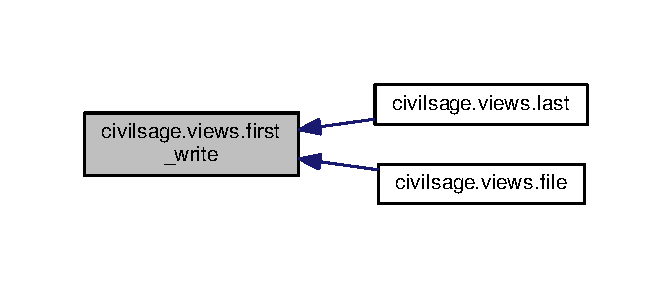
\includegraphics[width=322pt]{a00036_ad9397359f36a9df37e0aa43f3be032a3_icgraph}
\end{center}
\end{figure}


\hypertarget{a00036_a7b4fd4478a312ce8e35a192159c59de9}{}\index{civilsage\+::views@{civilsage\+::views}!index@{index}}
\index{index@{index}!civilsage\+::views@{civilsage\+::views}}
\subsubsection[{index(request)}]{\setlength{\rightskip}{0pt plus 5cm}def civilsage.\+views.\+index (
\begin{DoxyParamCaption}
\item[{}]{request}
\end{DoxyParamCaption}
)}\label{a00036_a7b4fd4478a312ce8e35a192159c59de9}
\begin{DoxyVerb}first veiw created by rendering html page
from templete
...
\end{DoxyVerb}
 

Definition at line 14 of file views.\+py.


\begin{DoxyCode}
14 \textcolor{keyword}{def }\hyperlink{a00036_a7b4fd4478a312ce8e35a192159c59de9}{index}(request):
15     \textcolor{stringliteral}{"""}
16 \textcolor{stringliteral}{    first veiw created by rendering html page}
17 \textcolor{stringliteral}{    from templete}
18 \textcolor{stringliteral}{    ...}
19 \textcolor{stringliteral}{    """}
20 
21     \textcolor{keywordflow}{return} render(request, \textcolor{stringliteral}{'civilsage/index.html'})
22 
\end{DoxyCode}
\hypertarget{a00036_aed47fb0740a2fa14693f697905788719}{}\index{civilsage\+::views@{civilsage\+::views}!last@{last}}
\index{last@{last}!civilsage\+::views@{civilsage\+::views}}
\subsubsection[{last(request)}]{\setlength{\rightskip}{0pt plus 5cm}def civilsage.\+views.\+last (
\begin{DoxyParamCaption}
\item[{}]{request}
\end{DoxyParamCaption}
)}\label{a00036_aed47fb0740a2fa14693f697905788719}
\begin{DoxyVerb}This function gets request from matix.html and
gives pdf as output to user
...
\end{DoxyVerb}
 

Definition at line 71 of file views.\+py.


\begin{DoxyCode}
71 \textcolor{keyword}{def }\hyperlink{a00036_aed47fb0740a2fa14693f697905788719}{last}(request):
72     \textcolor{stringliteral}{"""}
73 \textcolor{stringliteral}{}
74 \textcolor{stringliteral}{    This function gets request from matix.html and}
75 \textcolor{stringliteral}{    gives pdf as output to user}
76 \textcolor{stringliteral}{    ...}
77 \textcolor{stringliteral}{    """}
78 
79     message=\textcolor{stringliteral}{'error occured please fill again'}
80     \textcolor{keywordflow}{try}:
81         \textcolor{comment}{#calling function to writte basic input}
82         name,message=\hyperlink{a00036_ad9397359f36a9df37e0aa43f3be032a3}{first\_write}(request)
83         \textcolor{comment}{#getting numbers of storeys}
84         num = request.session.get(\textcolor{stringliteral}{'Number\_of\_storeys'})
85 
86         \textcolor{comment}{#opening input.sage to append remaining inputs}
87         command=name+\textcolor{stringliteral}{'/input.sage'}
88         file=open(command,\textcolor{stringliteral}{'a'})
89 
90         \textcolor{comment}{#list of basic tags}
91         var = [\textcolor{stringliteral}{'mass'},\textcolor{stringliteral}{'Height\_storey'},\textcolor{stringliteral}{'Stiffness\_storey'}]
92 
93         \textcolor{comment}{#writing matix into sage file}
94         \textcolor{keywordflow}{for} j \textcolor{keywordflow}{in} var:
95             file.write(j)
96             file.write(\textcolor{stringliteral}{'=matrix(['})
97 
98             \textcolor{comment}{#writing elements of matix}
99             \textcolor{keywordflow}{for} i \textcolor{keywordflow}{in} range(int(num)):
100 
101                 \textcolor{comment}{#creating input tags}
102                 temp = j+str(i)
103                 file.write(\textcolor{stringliteral}{'['})
104 
105                 \textcolor{comment}{#getting input from tags}
106                 d=request.POST.get(temp)
107                 file.write(d)
108                 file.write(\textcolor{stringliteral}{']'})
109 
110                 \textcolor{comment}{#condition to check last element}
111                 \hyperlink{a00029_ac2d69f5011896c6ed4a54e0dd36f6334}{if}( i!=int(num)-1):
112                     file.write(\textcolor{stringliteral}{','})
113             file.write(\textcolor{stringliteral}{'])\(\backslash\)n'})
114         file.close()
115 
116         \hyperlink{a00029_ac2d69f5011896c6ed4a54e0dd36f6334}{if}(request.POST.get(\textcolor{stringliteral}{'email\_id'})):
117             \textcolor{comment}{#calling funcion to send pdf and run that as background process}
118             thread = threading.Thread(target=pdfemail,args=(request,name))
119             thread.daemon = \textcolor{keyword}{True}
120             thread.start()
121             message=\textcolor{stringliteral}{"PDF send to "}+request.POST.get(\textcolor{stringliteral}{'email\_id'})
122             \textcolor{keywordflow}{return} render(request, \textcolor{stringliteral}{"civilsage/index.html"}, \{\textcolor{stringliteral}{'message'}:message\})
123         \textcolor{keywordflow}{else}:
124             \textcolor{comment}{#creating and writing sh file for background processing}
125             command=name+\textcolor{stringliteral}{'/civil.sh'}
126             file=open(command,\textcolor{stringliteral}{'w'})
127             command=\textcolor{stringliteral}{'cd '}+name
128             file.write(command)
129             file.write(\textcolor{stringliteral}{'\(\backslash\)nlatex civil.tex\(\backslash\)nsage civil.sagetex.sage\(\backslash\)n'})
130             file.write(\textcolor{stringliteral}{'pdflatex civil.tex\(\backslash\)n'})
131             file.close()
132 
133             \textcolor{comment}{#calling sh file for background processing}
134             command=\textcolor{stringliteral}{'sh '}+name+\textcolor{stringliteral}{'/civil.sh'}
135             os.system(command)
136 
137             \textcolor{comment}{#opening creted pdf to display to user}
138             command=name+\textcolor{stringliteral}{'/civil.pdf'}
139             f=open(command)
140 
141             \textcolor{comment}{#sending pdf as response}
142             response = HttpResponse(f,content\_type=\textcolor{stringliteral}{'application/pdf'})
143             response[\textcolor{stringliteral}{'Content-Disposition'}] = \textcolor{stringliteral}{'attachment; filename="civil.pdf"'}
144             \textcolor{comment}{#deleting temperary files}
145             command=\textcolor{stringliteral}{'rm -rf '}+name
146             os.system(command)
147             \textcolor{keywordflow}{return} response
148     \textcolor{keywordflow}{except}:
149         \textcolor{keywordflow}{return} render(request, \textcolor{stringliteral}{"civilsage/index.html"},
150         \{\textcolor{stringliteral}{'message'}:message,\textcolor{stringliteral}{'email\_get'}:request.session.get(\textcolor{stringliteral}{'email\_get'})\})
151 
152 
\end{DoxyCode}


Here is the call graph for this function\+:\nopagebreak
\begin{figure}[H]
\begin{center}
\leavevmode
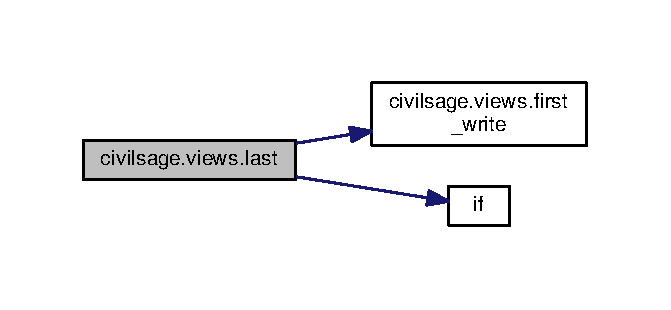
\includegraphics[width=322pt]{a00036_aed47fb0740a2fa14693f697905788719_cgraph}
\end{center}
\end{figure}


\hypertarget{a00036_a8b58c93a9c82e84143c43dafaa744a4b}{}\index{civilsage\+::views@{civilsage\+::views}!matrix@{matrix}}
\index{matrix@{matrix}!civilsage\+::views@{civilsage\+::views}}
\subsubsection[{matrix(request)}]{\setlength{\rightskip}{0pt plus 5cm}def civilsage.\+views.\+matrix (
\begin{DoxyParamCaption}
\item[{}]{request}
\end{DoxyParamCaption}
)}\label{a00036_a8b58c93a9c82e84143c43dafaa744a4b}
\begin{DoxyVerb}This function display matrix for input from user and take
response from index veiw and write input taken through index.html
and write in input.sage file
...
\end{DoxyVerb}
 

Definition at line 23 of file views.\+py.


\begin{DoxyCode}
23 \textcolor{keyword}{def }\hyperlink{a00036_a8b58c93a9c82e84143c43dafaa744a4b}{matrix}(request):
24     \textcolor{stringliteral}{"""}
25 \textcolor{stringliteral}{    This function display matrix for input from user and take}
26 \textcolor{stringliteral}{    response from index veiw and write input taken through index.html}
27 \textcolor{stringliteral}{    and write in input.sage file}
28 \textcolor{stringliteral}{    ...}
29 \textcolor{stringliteral}{    """}
30 
31     \textcolor{keywordflow}{try}:
32         \textcolor{comment}{#dictionary of all input tags}
33         lists = \{\textcolor{stringliteral}{'Soil\_type'}:\textcolor{stringliteral}{''},\textcolor{stringliteral}{'Number\_of\_storeys'}:\textcolor{stringliteral}{''}
34         ,\textcolor{stringliteral}{'Importance\_factor'}:\textcolor{stringliteral}{''},\textcolor{stringliteral}{'Response\_reduction\_factor'}:\textcolor{stringliteral}{''}
35         ,\textcolor{stringliteral}{'Zone\_factor'}:\textcolor{stringliteral}{''},\textcolor{stringliteral}{'Gravity\_acceleration'}:\textcolor{stringliteral}{''}
36         ,\textcolor{stringliteral}{'Modes\_considered'}:\textcolor{stringliteral}{''},\textcolor{stringliteral}{'email\_get'}:\textcolor{stringliteral}{''}\}
37 
38         name = \textcolor{stringliteral}{''}
39 
40         \textcolor{comment}{#getting input using tags and sending it as response}
41         \textcolor{keywordflow}{for} var \textcolor{keywordflow}{in} lists.keys():
42             request.session[var] = request.POST.get(var)
43 
44         \textcolor{comment}{#creating directory from base directory}
45         lists[\textcolor{stringliteral}{'Number\_of\_storeys'}] = request.POST.get(\textcolor{stringliteral}{'Number\_of\_storeys'})
46 
47         \textcolor{comment}{#making list for iteratation in templete}
48         number\_of\_storeys = list()
49         \textcolor{comment}{#name of directory of specific user}
50         \textcolor{keywordflow}{for} a \textcolor{keywordflow}{in} range(int(lists[\textcolor{stringliteral}{'Number\_of\_storeys'}])):
51             number\_of\_storeys.append(\textcolor{stringliteral}{'a'})
52 
53         \textcolor{comment}{#calling differnet veiws based on option whether}
54         \textcolor{comment}{#manually}
55 
56         \hyperlink{a00029_ac2d69f5011896c6ed4a54e0dd36f6334}{if}(request.POST.get(\textcolor{stringliteral}{'through\_file'})==\textcolor{stringliteral}{'Y'}):
57             \textcolor{keywordflow}{return} render( request,\textcolor{stringliteral}{'civilsage/file.html'}
58             ,\{\textcolor{stringliteral}{'number\_of\_storeys'}: number\_of\_storeys,
59             \textcolor{stringliteral}{'email\_get'}: request.POST.get(\textcolor{stringliteral}{'email\_get'})\})
60         \textcolor{keywordflow}{else}:
61         \textcolor{comment}{#user want to upload matrix value through file or}
62             \textcolor{keywordflow}{return} render( request,\textcolor{stringliteral}{'civilsage/matrix.html'}
63             ,\{\textcolor{stringliteral}{'number\_of\_storeys'}: number\_of\_storeys,
64             \textcolor{stringliteral}{'email\_get'}: request.POST.get(\textcolor{stringliteral}{'email\_get'}) \})
65     \textcolor{keywordflow}{except}:
66         \textcolor{keywordflow}{return} render(request, \textcolor{stringliteral}{'civilsage/index.html'}
67         ,\{\textcolor{stringliteral}{'message'}:\textcolor{stringliteral}{'please fill again'}\})
68 
69 
70 
\end{DoxyCode}


Here is the call graph for this function\+:\nopagebreak
\begin{figure}[H]
\begin{center}
\leavevmode
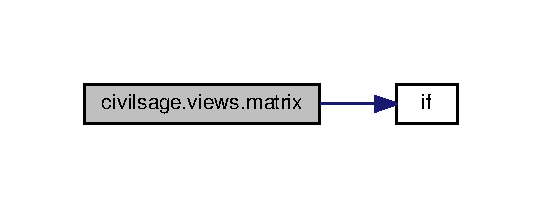
\includegraphics[width=260pt]{a00036_a8b58c93a9c82e84143c43dafaa744a4b_cgraph}
\end{center}
\end{figure}




Here is the caller graph for this function\+:\nopagebreak
\begin{figure}[H]
\begin{center}
\leavevmode
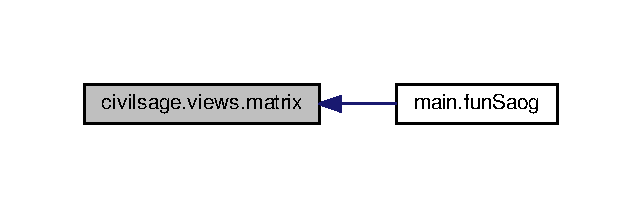
\includegraphics[width=308pt]{a00036_a8b58c93a9c82e84143c43dafaa744a4b_icgraph}
\end{center}
\end{figure}


\hypertarget{a00036_a9914ff19f8e15ccab1a07eaeac8cfb21}{}\index{civilsage\+::views@{civilsage\+::views}!pdfemail@{pdfemail}}
\index{pdfemail@{pdfemail}!civilsage\+::views@{civilsage\+::views}}
\subsubsection[{pdfemail(request, name)}]{\setlength{\rightskip}{0pt plus 5cm}def civilsage.\+views.\+pdfemail (
\begin{DoxyParamCaption}
\item[{}]{request, }
\item[{}]{name}
\end{DoxyParamCaption}
)}\label{a00036_a9914ff19f8e15ccab1a07eaeac8cfb21}
\begin{DoxyVerb}A function that run as background process to send pdf as emails
...
\end{DoxyVerb}
 

Definition at line 242 of file views.\+py.


\begin{DoxyCode}
242 \textcolor{keyword}{def }\hyperlink{a00036_a9914ff19f8e15ccab1a07eaeac8cfb21}{pdfemail}(request,name):
243     \textcolor{stringliteral}{"""}
244 \textcolor{stringliteral}{    A function that run as background process to send pdf as emails}
245 \textcolor{stringliteral}{    ...}
246 \textcolor{stringliteral}{    """}
247     message=\textcolor{stringliteral}{'unable to send'}
248     \textcolor{keywordflow}{try}:
249         \textcolor{comment}{#creating and writing sh file for background processing}
250         email\_id=request.POST.get(\textcolor{stringliteral}{'email\_id'})
251         command=name+\textcolor{stringliteral}{'/email.txt'}
252         f=open(command,\textcolor{stringliteral}{'w'})
253         f.write(email\_id)
254         f.close()
255         command=name+\textcolor{stringliteral}{'/civil.sh'}
256         file=open(command,\textcolor{stringliteral}{'w'})
257         command=\textcolor{stringliteral}{'cd '}+name
258         file.write(command)
259         file.write(\textcolor{stringliteral}{'\(\backslash\)nlatex civil.tex\(\backslash\)nsage civil.sagetex.sage\(\backslash\)n'})
260         file.write(\textcolor{stringliteral}{'pdflatex civil.tex\(\backslash\)n'})
261         file.close()
262         \textcolor{comment}{#calling sh file for background processing}
263         command=\textcolor{stringliteral}{'sh '}+name+\textcolor{stringliteral}{'/civil.sh'}
264         os.system(command)
265         command=name+\textcolor{stringliteral}{'/civil.pdf'}
266         email\_id=request.POST.get(\textcolor{stringliteral}{'email\_id'})
267         user\_email = EmailMessage(\textcolor{stringliteral}{'Dynamics of structure'},
268         \textcolor{stringliteral}{'You have is ready'}, to=[email\_id])
269         user\_email.attach\_file(command)
270         user\_email.send()
271         command=\textcolor{stringliteral}{'rm -rf '}+name
272         os.system(command)
273     \textcolor{keywordflow}{except}:
274         email\_id=request.POST.get(\textcolor{stringliteral}{'email\_id'})
275         user\_email = EmailMessage(\textcolor{stringliteral}{'Dynamics of structure'},
276         message, to=[email\_id])
277 
\end{DoxyCode}

\hypertarget{a00037}{}\section{initial\+\_\+file Namespace Reference}
\label{a00037}\index{initial\+\_\+file@{initial\+\_\+file}}
\subsection*{Functions}
\begin{DoxyCompactItemize}
\item 
def \hyperlink{a00037_a105b1aa7bf4db853b6f4d064ed224030}{pdfemail} ()
\end{DoxyCompactItemize}


\subsection{Function Documentation}
\hypertarget{a00037_a105b1aa7bf4db853b6f4d064ed224030}{}\index{initial\+\_\+file@{initial\+\_\+file}!pdfemail@{pdfemail}}
\index{pdfemail@{pdfemail}!initial\+\_\+file@{initial\+\_\+file}}
\subsubsection[{pdfemail()}]{\setlength{\rightskip}{0pt plus 5cm}def initial\+\_\+file.\+pdfemail (
\begin{DoxyParamCaption}
{}
\end{DoxyParamCaption}
)}\label{a00037_a105b1aa7bf4db853b6f4d064ed224030}


Definition at line 3 of file initial\+\_\+file.\+py.


\begin{DoxyCode}
3 \textcolor{keyword}{def }\hyperlink{a00037_a105b1aa7bf4db853b6f4d064ed224030}{pdfemail}():
4     os.system(\textcolor{stringliteral}{'sage sagemath/input.sage'})
5     
6 \end{DoxyCode}

\hypertarget{a00038}{}\section{input Namespace Reference}
\label{a00038}\index{input@{input}}
\subsection*{Variables}
\begin{DoxyCompactItemize}
\item 
tuple \hyperlink{a00038_ac1b86705df1981fd4962cc056fb0608a}{\+\_\+sage\+\_\+const\+\_\+9p8} = Real\+Number(\textquotesingle{}9.\+8\textquotesingle{})
\item 
\hyperlink{a00038_a55ab15c1c171513e99332aa50c723764}{Gravity\+\_\+acceleration} = \hyperlink{a00038_ac1b86705df1981fd4962cc056fb0608a}{\+\_\+sage\+\_\+const\+\_\+9p8}
\item 
\hyperlink{a00038_a0840d963ea24db338f3ab4457defb494}{Importance\+\_\+factor} = \+\_\+sage\+\_\+const\+\_\+1
\item 
\hyperlink{a00038_adb7aca4735796aaa4a46456d3edeac2e}{Modes\+\_\+considered} = \+\_\+sage\+\_\+const\+\_\+4
\item 
\hyperlink{a00038_a10237b312ba44e8c8090db86059c5803}{Number\+\_\+of\+\_\+storeys} = \+\_\+sage\+\_\+const\+\_\+4
\item 
\hyperlink{a00038_aa6d0078a6d934c0d515d85059525e938}{Response\+\_\+reduction\+\_\+factor} = \+\_\+sage\+\_\+const\+\_\+5
\item 
\hyperlink{a00038_a6221ae01cf2fb9e8cd22204749785a0e}{Soil\+\_\+type} = \+\_\+sage\+\_\+const\+\_\+1
\item 
\hyperlink{a00038_aeea70e58ec9bb0d3d6c4363867eb0f82}{Zone\+\_\+factor} = \+\_\+sage\+\_\+const\+\_\+0p24
\end{DoxyCompactItemize}


\subsection{Variable Documentation}
\hypertarget{a00038_ac1b86705df1981fd4962cc056fb0608a}{}\index{input@{input}!\+\_\+sage\+\_\+const\+\_\+9p8@{\+\_\+sage\+\_\+const\+\_\+9p8}}
\index{\+\_\+sage\+\_\+const\+\_\+9p8@{\+\_\+sage\+\_\+const\+\_\+9p8}!input@{input}}
\subsubsection[{\+\_\+sage\+\_\+const\+\_\+9p8}]{\setlength{\rightskip}{0pt plus 5cm}tuple input.\+\_\+sage\+\_\+const\+\_\+9p8 = Real\+Number(\textquotesingle{}9.\+8\textquotesingle{})}\label{a00038_ac1b86705df1981fd4962cc056fb0608a}


Definition at line 3 of file input.\+sage.\+py.

\hypertarget{a00038_a55ab15c1c171513e99332aa50c723764}{}\index{input@{input}!Gravity\+\_\+acceleration@{Gravity\+\_\+acceleration}}
\index{Gravity\+\_\+acceleration@{Gravity\+\_\+acceleration}!input@{input}}
\subsubsection[{Gravity\+\_\+acceleration}]{\setlength{\rightskip}{0pt plus 5cm}input.\+Gravity\+\_\+acceleration = {\bf \+\_\+sage\+\_\+const\+\_\+9p8}}\label{a00038_a55ab15c1c171513e99332aa50c723764}


Definition at line 7 of file input.\+sage.\+py.

\hypertarget{a00038_a0840d963ea24db338f3ab4457defb494}{}\index{input@{input}!Importance\+\_\+factor@{Importance\+\_\+factor}}
\index{Importance\+\_\+factor@{Importance\+\_\+factor}!input@{input}}
\subsubsection[{Importance\+\_\+factor}]{\setlength{\rightskip}{0pt plus 5cm}input.\+Importance\+\_\+factor = \+\_\+sage\+\_\+const\+\_\+1}\label{a00038_a0840d963ea24db338f3ab4457defb494}


Definition at line 5 of file input.\+sage.\+py.

\hypertarget{a00038_adb7aca4735796aaa4a46456d3edeac2e}{}\index{input@{input}!Modes\+\_\+considered@{Modes\+\_\+considered}}
\index{Modes\+\_\+considered@{Modes\+\_\+considered}!input@{input}}
\subsubsection[{Modes\+\_\+considered}]{\setlength{\rightskip}{0pt plus 5cm}input.\+Modes\+\_\+considered = \+\_\+sage\+\_\+const\+\_\+4}\label{a00038_adb7aca4735796aaa4a46456d3edeac2e}


Definition at line 8 of file input.\+sage.\+py.

\hypertarget{a00038_a10237b312ba44e8c8090db86059c5803}{}\index{input@{input}!Number\+\_\+of\+\_\+storeys@{Number\+\_\+of\+\_\+storeys}}
\index{Number\+\_\+of\+\_\+storeys@{Number\+\_\+of\+\_\+storeys}!input@{input}}
\subsubsection[{Number\+\_\+of\+\_\+storeys}]{\setlength{\rightskip}{0pt plus 5cm}input.\+Number\+\_\+of\+\_\+storeys = \+\_\+sage\+\_\+const\+\_\+4}\label{a00038_a10237b312ba44e8c8090db86059c5803}


Definition at line 6 of file input.\+sage.\+py.

\hypertarget{a00038_aa6d0078a6d934c0d515d85059525e938}{}\index{input@{input}!Response\+\_\+reduction\+\_\+factor@{Response\+\_\+reduction\+\_\+factor}}
\index{Response\+\_\+reduction\+\_\+factor@{Response\+\_\+reduction\+\_\+factor}!input@{input}}
\subsubsection[{Response\+\_\+reduction\+\_\+factor}]{\setlength{\rightskip}{0pt plus 5cm}input.\+Response\+\_\+reduction\+\_\+factor = \+\_\+sage\+\_\+const\+\_\+5}\label{a00038_aa6d0078a6d934c0d515d85059525e938}


Definition at line 9 of file input.\+sage.\+py.

\hypertarget{a00038_a6221ae01cf2fb9e8cd22204749785a0e}{}\index{input@{input}!Soil\+\_\+type@{Soil\+\_\+type}}
\index{Soil\+\_\+type@{Soil\+\_\+type}!input@{input}}
\subsubsection[{Soil\+\_\+type}]{\setlength{\rightskip}{0pt plus 5cm}input.\+Soil\+\_\+type = \+\_\+sage\+\_\+const\+\_\+1}\label{a00038_a6221ae01cf2fb9e8cd22204749785a0e}


Definition at line 4 of file input.\+sage.\+py.

\hypertarget{a00038_aeea70e58ec9bb0d3d6c4363867eb0f82}{}\index{input@{input}!Zone\+\_\+factor@{Zone\+\_\+factor}}
\index{Zone\+\_\+factor@{Zone\+\_\+factor}!input@{input}}
\subsubsection[{Zone\+\_\+factor}]{\setlength{\rightskip}{0pt plus 5cm}input.\+Zone\+\_\+factor = \+\_\+sage\+\_\+const\+\_\+0p24}\label{a00038_aeea70e58ec9bb0d3d6c4363867eb0f82}


Definition at line 10 of file input.\+sage.\+py.


\hypertarget{a00039}{}\section{main Namespace Reference}
\label{a00039}\index{main@{main}}
\subsection*{Functions}
\begin{DoxyCompactItemize}
\item 
def \hyperlink{a00039_a4f60afd2426ee9409955e4352b3f0486}{fun\+Saog} (soil\+Type, time\+Prd)
\end{DoxyCompactItemize}
\subsection*{Variables}
\begin{DoxyCompactItemize}
\item 
tuple \hyperlink{a00039_ad85d7913c0e40b9e1f30e64611a0fafa}{\+\_\+sage\+\_\+const\+\_\+2} = Integer(2)
\item 
tuple \hyperlink{a00039_ad101f166a53497f04b37636bcadbfe65}{A} = \hyperlink{a00039_a0011be18dbc87087d6aaf28802f121c0}{Stiffness\+\_\+matrix}$\ast$Mass.\+inverse()
\item 
tuple \hyperlink{a00039_a90e3156cc1a3ea63ba2d089e78b34e3d}{A\+\_\+h} = zero\+\_\+matrix(R\+R,Number\+\_\+of\+\_\+storeys,Number\+\_\+of\+\_\+storeys)
\item 
tuple \hyperlink{a00039_a6ae8768d11174f5baf9febc5244d6f06}{B} = zero\+\_\+matrix(R\+R,Number\+\_\+of\+\_\+storeys,Number\+\_\+of\+\_\+storeys)
\item 
list \hyperlink{a00039_ab1e783015bffd2e1d395a9099143d967}{b} = \+\_\+sage\+\_\+const\+\_\+1+\hyperlink{a00039_a6ae8768d11174f5baf9febc5244d6f06}{B}\mbox{[}\hyperlink{a00008_a6dbbc96f4222af2f6c18c8e60f41726b}{i},\hyperlink{a00008_ac86694252f8dfdb19aaeadc4b7c342c6}{j}\mbox{]}
\item 
tuple \hyperlink{a00039_aeabbf69db1809807f065c2d1e9a62567}{color} = hue(\+\_\+sage\+\_\+const\+\_\+0p4 + \+\_\+sage\+\_\+const\+\_\+0p6 $\ast$(\hyperlink{a00008_a6dbbc96f4222af2f6c18c8e60f41726b}{i}/\+\_\+sage\+\_\+const\+\_\+10 ))
\item 
tuple \hyperlink{a00039_a35df7d294c439792977f174dd5b04ec1}{Design\+\_\+lateral\+\_\+force} = zero\+\_\+matrix(R\+R,Number\+\_\+of\+\_\+storeys,Number\+\_\+of\+\_\+storeys)
\item 
tuple \hyperlink{a00039_aa7f4fe671f919f7f067f9337ef9e02c0}{e} = (\+\_\+sage\+\_\+const\+\_\+1 -\/\hyperlink{a00039_a6ae8768d11174f5baf9febc5244d6f06}{B}\mbox{[}\hyperlink{a00008_a6dbbc96f4222af2f6c18c8e60f41726b}{i},\hyperlink{a00008_ac86694252f8dfdb19aaeadc4b7c342c6}{j}\mbox{]}$\ast$$\ast$\hyperlink{a00039_ad85d7913c0e40b9e1f30e64611a0fafa}{\+\_\+sage\+\_\+const\+\_\+2} )
\item 
tuple \hyperlink{a00039_a4612305e50326c88dea04736a647c238}{Force} = zero\+\_\+vector(R\+R,Number\+\_\+of\+\_\+storeys)
\item 
tuple \hyperlink{a00039_ad40f6b3437e83a0385177ac65a317b97}{Graph} = plot(\mbox{[}$\,$\mbox{]})
\item 
tuple \hyperlink{a00039_a00488f5887e168f7781b6fb94dd08518}{J} = zero\+\_\+vector(R\+R,Number\+\_\+of\+\_\+storeys)
\item 
list \hyperlink{a00039_a027916efc284622d928c1d8383917f6d}{l} = \hyperlink{a00039_a6461376590c833b81e5920e96ed3d5bf}{Peak\+\_\+shear\+\_\+force}\mbox{[}\+:,\hyperlink{a00008_a6dbbc96f4222af2f6c18c8e60f41726b}{i}\mbox{]}
\item 
tuple \hyperlink{a00039_a8d395a4120126cf1de1d3f04b1fc3457}{Lateral\+\_\+force} = zero\+\_\+vector(R\+R,Number\+\_\+of\+\_\+storeys)
\item 
tuple \hyperlink{a00039_aa6efadb1dc89cc9d5b75113b025fe962}{Level\+\_\+floor} = zero\+\_\+vector(R\+R,Number\+\_\+of\+\_\+storeys)
\item 
list \hyperlink{a00039_af6e3698b7f50fc004eb759d7c447fdb3}{m} = \hyperlink{a00039_a5eac8e4368036ef94463d6e42c1628c5}{X}\mbox{[}\hyperlink{a00008_ac86694252f8dfdb19aaeadc4b7c342c6}{j},\+:\mbox{]}
\item 
tuple \hyperlink{a00039_a70551c7fc78da8fdec83fe500056d388}{mid} = \hyperlink{a00039_a1787a37505189f764069a45071189112}{q}$\ast$Mass$\ast$q.\+transpose()
\item 
tuple \hyperlink{a00039_ae8c706be82800a75da37e5da67018f90}{Modal\+\_\+contribution} = list()
\item 
tuple \hyperlink{a00039_ac7e5d737af53772a131628449c0e6477}{Modal\+\_\+mass} = list()
\item 
tuple \hyperlink{a00039_a4ad22e0a1336b0e665ff865d68f4fcc1}{Modal\+\_\+participation\+\_\+factor} = list()
\item 
\hyperlink{a00039_a9d22ac077c22a97b1b095068a1500d16}{Modes\+\_\+considered} = Number\+\_\+of\+\_\+modes\+\_\+to\+\_\+be\+\_\+considered
\item 
tuple \hyperlink{a00039_a0cc58897a39912c706ab64fd26e0d62e}{Omega} = zero\+\_\+vector(R\+R,Number\+\_\+of\+\_\+storeys)
\item 
tuple \hyperlink{a00039_abc7a524ddae98db1c2f4cf8535104feb}{Omega\+\_\+square} = A.\+eigenvalues()
\item 
tuple \hyperlink{a00039_ad403610ba53df02f8dfaff8dd64227b3}{P} = zero\+\_\+matrix(R\+R,Number\+\_\+of\+\_\+storeys,Number\+\_\+of\+\_\+storeys)
\item 
tuple \hyperlink{a00039_ab31fc16b432d2248a6c76c6a18d741d0}{p} = list()
\item 
list \hyperlink{a00039_add7e0394c94a2e2115aff785eb6995e3}{P1} = P1+Mass\mbox{[}\hyperlink{a00008_a6dbbc96f4222af2f6c18c8e60f41726b}{i}\mbox{]}
\item 
list \hyperlink{a00039_a1b83b7a3849a8e1c84b9906c45625fec}{P2} = P2+Mass\mbox{[}\hyperlink{a00008_a6dbbc96f4222af2f6c18c8e60f41726b}{i}\mbox{]}
\item 
tuple \hyperlink{a00039_a6461376590c833b81e5920e96ed3d5bf}{Peak\+\_\+shear\+\_\+force} = zero\+\_\+matrix(R\+R,Number\+\_\+of\+\_\+storeys, Number\+\_\+of\+\_\+storeys)
\item 
tuple \hyperlink{a00039_a1787a37505189f764069a45071189112}{q} = \hyperlink{a00039_a0011be18dbc87087d6aaf28802f121c0}{Stiffness\+\_\+matrix}-\/(\hyperlink{a00039_af76005101c339a32cd5d37ba82ee072c}{w}$\ast$$\ast$\hyperlink{a00039_ad85d7913c0e40b9e1f30e64611a0fafa}{\+\_\+sage\+\_\+const\+\_\+2} )
\item 
list \hyperlink{a00039_a4760f4121f66000c5570f75176649cb8}{r} = \hyperlink{a00039_a0cc58897a39912c706ab64fd26e0d62e}{Omega}\mbox{[}\hyperlink{a00008_ac86694252f8dfdb19aaeadc4b7c342c6}{j}\mbox{]}
\item 
tuple \hyperlink{a00039_a01374e7fea2c00172c845c7a5c71cfae}{Sa\+\_\+by\+\_\+g} = zero\+\_\+matrix(R\+R,Number\+\_\+of\+\_\+storeys,Number\+\_\+of\+\_\+storeys)
\item 
tuple \hyperlink{a00039_a0011be18dbc87087d6aaf28802f121c0}{Stiffness\+\_\+matrix} = zero\+\_\+matrix(Q\+Q,Number\+\_\+of\+\_\+storeys,Number\+\_\+of\+\_\+storeys)
\item 
tuple \hyperlink{a00039_aaa52e7055409dcf0785880422294a704}{Storey\+\_\+shear\+\_\+force} = zero\+\_\+vector(R\+R,Number\+\_\+of\+\_\+storeys)
\item 
tuple \hyperlink{a00039_ad9f40bb3020e00eecaf17c078a1e61b6}{Storey\+\_\+shear\+\_\+force2} = zero\+\_\+vector(R\+R,Number\+\_\+of\+\_\+storeys)
\item 
\hyperlink{a00039_a27fb93072b84fd448623807df350f132}{sum\+\_\+modal\+\_\+mass} = \+\_\+sage\+\_\+const\+\_\+0
\item 
tuple \hyperlink{a00039_a76fa8360c88818d30b9b5d2a473e79e4}{Time\+\_\+period} = zero\+\_\+matrix(R\+R,Number\+\_\+of\+\_\+storeys,Number\+\_\+of\+\_\+storeys)
\item 
tuple \hyperlink{a00039_afe9c3a972582e300106b7dec57600887}{Time\+\_\+periods} = list()
\item 
string \hyperlink{a00039_a52e65712caa18dade1326ad4efeebfa1}{Type\+\_\+of\+\_\+soil} = \textquotesingle{}\textquotesingle{}
\item 
tuple \hyperlink{a00039_af76005101c339a32cd5d37ba82ee072c}{w} = var(\textquotesingle{}w\textquotesingle{})
\item 
tuple \hyperlink{a00039_a5eac8e4368036ef94463d6e42c1628c5}{X} = zero\+\_\+matrix(R\+R,Number\+\_\+of\+\_\+storeys,Number\+\_\+of\+\_\+storeys)
\item 
tuple \hyperlink{a00039_ae18df6a00aee4516c7ad8961b666e2a3}{X\+X} = X.\+transpose()
\item 
tuple \hyperlink{a00039_a2d5b336e3b2f7d2e14f04fa3cc413457}{z} = A.\+eigenvectors\+\_\+left()
\end{DoxyCompactItemize}


\subsection{Function Documentation}
\hypertarget{a00039_a4f60afd2426ee9409955e4352b3f0486}{}\index{main@{main}!fun\+Saog@{fun\+Saog}}
\index{fun\+Saog@{fun\+Saog}!main@{main}}
\subsubsection[{fun\+Saog(soil\+Type, time\+Prd)}]{\setlength{\rightskip}{0pt plus 5cm}def main.\+fun\+Saog (
\begin{DoxyParamCaption}
\item[{}]{soil\+Type, }
\item[{}]{time\+Prd}
\end{DoxyParamCaption}
)}\label{a00039_a4f60afd2426ee9409955e4352b3f0486}
\begin{DoxyVerb}function to pick values according to
type of soil selected
...
\end{DoxyVerb}
 

Definition at line 10 of file main.\+sage.\+py.


\begin{DoxyCode}
10 \textcolor{keyword}{def }\hyperlink{a00039_a4f60afd2426ee9409955e4352b3f0486}{funSaog}(soilType, timePrd):
11   \textcolor{stringliteral}{"""}
12 \textcolor{stringliteral}{  function to pick values according to}
13 \textcolor{stringliteral}{  type of soil selected}
14 \textcolor{stringliteral}{  ...}
15 \textcolor{stringliteral}{  """}
16   t1 = \_sage\_const\_0 ; t2 = \_sage\_const\_0 ; t3 = \_sage\_const\_0 ; t4 = \_sage\_const\_0 
17   eq3num = \_sage\_const\_0 
18   t2 = \_sage\_const\_0p10 
19   \hyperlink{a00029_ac2d69f5011896c6ed4a54e0dd36f6334}{if}(soilType==\textcolor{stringliteral}{'I'}):
20       t3 = \_sage\_const\_0p40 ; eq3num = \_sage\_const\_1p0 
21   \textcolor{keywordflow}{elif} (soilType==\textcolor{stringliteral}{'II'}):
22       t3 = \_sage\_const\_0p55 ; eq3num = \_sage\_const\_1p36 
23   elif(soilType==\textcolor{stringliteral}{'III'}):
24       t3 = \_sage\_const\_0p67 ; eq3num = \_sage\_const\_1p67 
25   \textcolor{keywordflow}{else}:
26       Print(\textcolor{stringliteral}{'Unexpected soil type'})
27   \textcolor{keywordflow}{if} (timePrd < t2):
28       sag = \_sage\_const\_1p  + \_sage\_const\_15  * timePrd
29   elif(timePrd > t3):
30       sag = eq3num / timePrd
31   \textcolor{keywordflow}{else}:
32       sag = \_sage\_const\_2p5 
33   \textcolor{keywordflow}{return} sag
34 
35 \textcolor{stringliteral}{"""main program ... """}
36 \textcolor{comment}{#loading input variables from input.sage}
37 load(\textcolor{stringliteral}{'input.sage'})
38 \textcolor{comment}{#changing style of brackets for latex output}
39 latex.matrix\_delimiters(\textcolor{stringliteral}{"["},\textcolor{stringliteral}{"]"})
40 latex.vector\_delimiters(\textcolor{stringliteral}{"["},\textcolor{stringliteral}{"]"})
41 
42 \textcolor{comment}{#converting mass in diagonal matrix}
43 Mass=\hyperlink{a00036_a8b58c93a9c82e84143c43dafaa744a4b}{matrix}(Number\_of\_storeys,Number\_of\_storeys)
\end{DoxyCode}


Here is the call graph for this function\+:\nopagebreak
\begin{figure}[H]
\begin{center}
\leavevmode
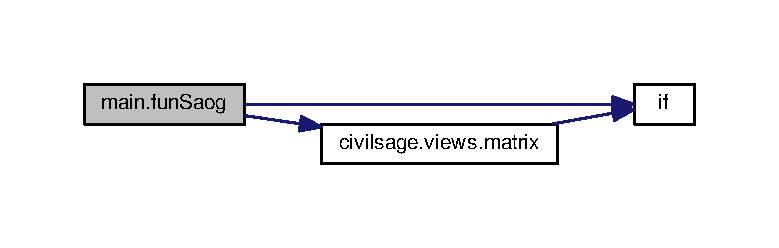
\includegraphics[width=350pt]{a00039_a4f60afd2426ee9409955e4352b3f0486_cgraph}
\end{center}
\end{figure}




\subsection{Variable Documentation}
\hypertarget{a00039_ad85d7913c0e40b9e1f30e64611a0fafa}{}\index{main@{main}!\+\_\+sage\+\_\+const\+\_\+2@{\+\_\+sage\+\_\+const\+\_\+2}}
\index{\+\_\+sage\+\_\+const\+\_\+2@{\+\_\+sage\+\_\+const\+\_\+2}!main@{main}}
\subsubsection[{\+\_\+sage\+\_\+const\+\_\+2}]{\setlength{\rightskip}{0pt plus 5cm}tuple main.\+\_\+sage\+\_\+const\+\_\+2 = Integer(2)}\label{a00039_ad85d7913c0e40b9e1f30e64611a0fafa}


Definition at line 3 of file main.\+sage.\+py.

\hypertarget{a00039_ad101f166a53497f04b37636bcadbfe65}{}\index{main@{main}!A@{A}}
\index{A@{A}!main@{main}}
\subsubsection[{A}]{\setlength{\rightskip}{0pt plus 5cm}tuple main.\+A = {\bf Stiffness\+\_\+matrix}$\ast$Mass.\+inverse()}\label{a00039_ad101f166a53497f04b37636bcadbfe65}


Definition at line 73 of file main.\+sage.\+py.

\hypertarget{a00039_a90e3156cc1a3ea63ba2d089e78b34e3d}{}\index{main@{main}!A\+\_\+h@{A\+\_\+h}}
\index{A\+\_\+h@{A\+\_\+h}!main@{main}}
\subsubsection[{A\+\_\+h}]{\setlength{\rightskip}{0pt plus 5cm}tuple main.\+A\+\_\+h = zero\+\_\+matrix(R\+R,Number\+\_\+of\+\_\+storeys,Number\+\_\+of\+\_\+storeys)}\label{a00039_a90e3156cc1a3ea63ba2d089e78b34e3d}


Definition at line 131 of file main.\+sage.\+py.

\hypertarget{a00039_a6ae8768d11174f5baf9febc5244d6f06}{}\index{main@{main}!B@{B}}
\index{B@{B}!main@{main}}
\subsubsection[{B}]{\setlength{\rightskip}{0pt plus 5cm}tuple main.\+B = zero\+\_\+matrix(R\+R,Number\+\_\+of\+\_\+storeys,Number\+\_\+of\+\_\+storeys)}\label{a00039_a6ae8768d11174f5baf9febc5244d6f06}


Definition at line 173 of file main.\+sage.\+py.

\hypertarget{a00039_ab1e783015bffd2e1d395a9099143d967}{}\index{main@{main}!b@{b}}
\index{b@{b}!main@{main}}
\subsubsection[{b}]{\setlength{\rightskip}{0pt plus 5cm}list main.\+b = \+\_\+sage\+\_\+const\+\_\+1+{\bf B}\mbox{[}{\bf i},{\bf j}\mbox{]}}\label{a00039_ab1e783015bffd2e1d395a9099143d967}


Definition at line 183 of file main.\+sage.\+py.

\hypertarget{a00039_aeabbf69db1809807f065c2d1e9a62567}{}\index{main@{main}!color@{color}}
\index{color@{color}!main@{main}}
\subsubsection[{color}]{\setlength{\rightskip}{0pt plus 5cm}tuple main.\+color = hue(\+\_\+sage\+\_\+const\+\_\+0p4 + \+\_\+sage\+\_\+const\+\_\+0p6 $\ast$({\bf i}/\+\_\+sage\+\_\+const\+\_\+10 ))}\label{a00039_aeabbf69db1809807f065c2d1e9a62567}


Definition at line 204 of file main.\+sage.\+py.

\hypertarget{a00039_a35df7d294c439792977f174dd5b04ec1}{}\index{main@{main}!Design\+\_\+lateral\+\_\+force@{Design\+\_\+lateral\+\_\+force}}
\index{Design\+\_\+lateral\+\_\+force@{Design\+\_\+lateral\+\_\+force}!main@{main}}
\subsubsection[{Design\+\_\+lateral\+\_\+force}]{\setlength{\rightskip}{0pt plus 5cm}tuple main.\+Design\+\_\+lateral\+\_\+force = zero\+\_\+matrix(R\+R,Number\+\_\+of\+\_\+storeys,Number\+\_\+of\+\_\+storeys)}\label{a00039_a35df7d294c439792977f174dd5b04ec1}


Definition at line 142 of file main.\+sage.\+py.

\hypertarget{a00039_aa7f4fe671f919f7f067f9337ef9e02c0}{}\index{main@{main}!e@{e}}
\index{e@{e}!main@{main}}
\subsubsection[{e}]{\setlength{\rightskip}{0pt plus 5cm}tuple main.\+e = (\+\_\+sage\+\_\+const\+\_\+1 -\/{\bf B}\mbox{[}{\bf i},{\bf j}\mbox{]}$\ast$$\ast${\bf \+\_\+sage\+\_\+const\+\_\+2} )}\label{a00039_aa7f4fe671f919f7f067f9337ef9e02c0}


Definition at line 185 of file main.\+sage.\+py.

\hypertarget{a00039_a4612305e50326c88dea04736a647c238}{}\index{main@{main}!Force@{Force}}
\index{Force@{Force}!main@{main}}
\subsubsection[{Force}]{\setlength{\rightskip}{0pt plus 5cm}tuple main.\+Force = zero\+\_\+vector(R\+R,Number\+\_\+of\+\_\+storeys)}\label{a00039_a4612305e50326c88dea04736a647c238}


Definition at line 191 of file main.\+sage.\+py.

\hypertarget{a00039_ad40f6b3437e83a0385177ac65a317b97}{}\index{main@{main}!Graph@{Graph}}
\index{Graph@{Graph}!main@{main}}
\subsubsection[{Graph}]{\setlength{\rightskip}{0pt plus 5cm}list main.\+Graph = plot(\mbox{[}$\,$\mbox{]})}\label{a00039_ad40f6b3437e83a0385177ac65a317b97}


Definition at line 209 of file main.\+sage.\+py.

\hypertarget{a00039_a00488f5887e168f7781b6fb94dd08518}{}\index{main@{main}!J@{J}}
\index{J@{J}!main@{main}}
\subsubsection[{J}]{\setlength{\rightskip}{0pt plus 5cm}tuple main.\+J = zero\+\_\+vector(R\+R,Number\+\_\+of\+\_\+storeys)}\label{a00039_a00488f5887e168f7781b6fb94dd08518}


Definition at line 91 of file main.\+sage.\+py.

\hypertarget{a00039_a027916efc284622d928c1d8383917f6d}{}\index{main@{main}!l@{l}}
\index{l@{l}!main@{main}}
\subsubsection[{l}]{\setlength{\rightskip}{0pt plus 5cm}list main.\+l = {\bf Peak\+\_\+shear\+\_\+force}\mbox{[}\+:,{\bf i}\mbox{]}}\label{a00039_a027916efc284622d928c1d8383917f6d}


Definition at line 189 of file main.\+sage.\+py.

\hypertarget{a00039_a8d395a4120126cf1de1d3f04b1fc3457}{}\index{main@{main}!Lateral\+\_\+force@{Lateral\+\_\+force}}
\index{Lateral\+\_\+force@{Lateral\+\_\+force}!main@{main}}
\subsubsection[{Lateral\+\_\+force}]{\setlength{\rightskip}{0pt plus 5cm}tuple main.\+Lateral\+\_\+force = zero\+\_\+vector(R\+R,Number\+\_\+of\+\_\+storeys)}\label{a00039_a8d395a4120126cf1de1d3f04b1fc3457}


Definition at line 187 of file main.\+sage.\+py.

\hypertarget{a00039_aa6efadb1dc89cc9d5b75113b025fe962}{}\index{main@{main}!Level\+\_\+floor@{Level\+\_\+floor}}
\index{Level\+\_\+floor@{Level\+\_\+floor}!main@{main}}
\subsubsection[{Level\+\_\+floor}]{\setlength{\rightskip}{0pt plus 5cm}tuple main.\+Level\+\_\+floor = zero\+\_\+vector(R\+R,Number\+\_\+of\+\_\+storeys)}\label{a00039_aa6efadb1dc89cc9d5b75113b025fe962}


Definition at line 51 of file main.\+sage.\+py.

\hypertarget{a00039_af6e3698b7f50fc004eb759d7c447fdb3}{}\index{main@{main}!m@{m}}
\index{m@{m}!main@{main}}
\subsubsection[{m}]{\setlength{\rightskip}{0pt plus 5cm}list main.\+m = {\bf X}\mbox{[}{\bf j},\+:\mbox{]}}\label{a00039_af6e3698b7f50fc004eb759d7c447fdb3}


Definition at line 112 of file main.\+sage.\+py.

\hypertarget{a00039_a70551c7fc78da8fdec83fe500056d388}{}\index{main@{main}!mid@{mid}}
\index{mid@{mid}!main@{main}}
\subsubsection[{mid}]{\setlength{\rightskip}{0pt plus 5cm}tuple main.\+mid = {\bf q}$\ast$Mass$\ast$q.\+transpose()}\label{a00039_a70551c7fc78da8fdec83fe500056d388}


Definition at line 95 of file main.\+sage.\+py.

\hypertarget{a00039_ae8c706be82800a75da37e5da67018f90}{}\index{main@{main}!Modal\+\_\+contribution@{Modal\+\_\+contribution}}
\index{Modal\+\_\+contribution@{Modal\+\_\+contribution}!main@{main}}
\subsubsection[{Modal\+\_\+contribution}]{\setlength{\rightskip}{0pt plus 5cm}tuple main.\+Modal\+\_\+contribution = list()}\label{a00039_ae8c706be82800a75da37e5da67018f90}


Definition at line 121 of file main.\+sage.\+py.

\hypertarget{a00039_ac7e5d737af53772a131628449c0e6477}{}\index{main@{main}!Modal\+\_\+mass@{Modal\+\_\+mass}}
\index{Modal\+\_\+mass@{Modal\+\_\+mass}!main@{main}}
\subsubsection[{Modal\+\_\+mass}]{\setlength{\rightskip}{0pt plus 5cm}tuple main.\+Modal\+\_\+mass = list()}\label{a00039_ac7e5d737af53772a131628449c0e6477}


Definition at line 108 of file main.\+sage.\+py.

\hypertarget{a00039_a4ad22e0a1336b0e665ff865d68f4fcc1}{}\index{main@{main}!Modal\+\_\+participation\+\_\+factor@{Modal\+\_\+participation\+\_\+factor}}
\index{Modal\+\_\+participation\+\_\+factor@{Modal\+\_\+participation\+\_\+factor}!main@{main}}
\subsubsection[{Modal\+\_\+participation\+\_\+factor}]{\setlength{\rightskip}{0pt plus 5cm}tuple main.\+Modal\+\_\+participation\+\_\+factor = list()}\label{a00039_a4ad22e0a1336b0e665ff865d68f4fcc1}


Definition at line 107 of file main.\+sage.\+py.

\hypertarget{a00039_a9d22ac077c22a97b1b095068a1500d16}{}\index{main@{main}!Modes\+\_\+considered@{Modes\+\_\+considered}}
\index{Modes\+\_\+considered@{Modes\+\_\+considered}!main@{main}}
\subsubsection[{Modes\+\_\+considered}]{\setlength{\rightskip}{0pt plus 5cm}main.\+Modes\+\_\+considered = Number\+\_\+of\+\_\+modes\+\_\+to\+\_\+be\+\_\+considered}\label{a00039_a9d22ac077c22a97b1b095068a1500d16}


Definition at line 164 of file main.\+sage.\+py.

\hypertarget{a00039_a0cc58897a39912c706ab64fd26e0d62e}{}\index{main@{main}!Omega@{Omega}}
\index{Omega@{Omega}!main@{main}}
\subsubsection[{Omega}]{\setlength{\rightskip}{0pt plus 5cm}tuple main.\+Omega = zero\+\_\+vector(R\+R,Number\+\_\+of\+\_\+storeys)}\label{a00039_a0cc58897a39912c706ab64fd26e0d62e}


Definition at line 77 of file main.\+sage.\+py.

\hypertarget{a00039_abc7a524ddae98db1c2f4cf8535104feb}{}\index{main@{main}!Omega\+\_\+square@{Omega\+\_\+square}}
\index{Omega\+\_\+square@{Omega\+\_\+square}!main@{main}}
\subsubsection[{Omega\+\_\+square}]{\setlength{\rightskip}{0pt plus 5cm}tuple main.\+Omega\+\_\+square = A.\+eigenvalues()}\label{a00039_abc7a524ddae98db1c2f4cf8535104feb}


Definition at line 74 of file main.\+sage.\+py.

\hypertarget{a00039_ad403610ba53df02f8dfaff8dd64227b3}{}\index{main@{main}!P@{P}}
\index{P@{P}!main@{main}}
\subsubsection[{P}]{\setlength{\rightskip}{0pt plus 5cm}tuple main.\+P = zero\+\_\+matrix(R\+R,Number\+\_\+of\+\_\+storeys,Number\+\_\+of\+\_\+storeys)}\label{a00039_ad403610ba53df02f8dfaff8dd64227b3}


Definition at line 172 of file main.\+sage.\+py.

\hypertarget{a00039_ab31fc16b432d2248a6c76c6a18d741d0}{}\index{main@{main}!p@{p}}
\index{p@{p}!main@{main}}
\subsubsection[{p}]{\setlength{\rightskip}{0pt plus 5cm}tuple main.\+p = list()}\label{a00039_ab31fc16b432d2248a6c76c6a18d741d0}


Definition at line 199 of file main.\+sage.\+py.

\hypertarget{a00039_add7e0394c94a2e2115aff785eb6995e3}{}\index{main@{main}!P1@{P1}}
\index{P1@{P1}!main@{main}}
\subsubsection[{P1}]{\setlength{\rightskip}{0pt plus 5cm}list main.\+P1 = P1+Mass\mbox{[}{\bf i}\mbox{]}}\label{a00039_add7e0394c94a2e2115aff785eb6995e3}


Definition at line 114 of file main.\+sage.\+py.

\hypertarget{a00039_a1b83b7a3849a8e1c84b9906c45625fec}{}\index{main@{main}!P2@{P2}}
\index{P2@{P2}!main@{main}}
\subsubsection[{P2}]{\setlength{\rightskip}{0pt plus 5cm}list main.\+P2 = P2+Mass\mbox{[}{\bf i}\mbox{]}}\label{a00039_a1b83b7a3849a8e1c84b9906c45625fec}


Definition at line 115 of file main.\+sage.\+py.

\hypertarget{a00039_a6461376590c833b81e5920e96ed3d5bf}{}\index{main@{main}!Peak\+\_\+shear\+\_\+force@{Peak\+\_\+shear\+\_\+force}}
\index{Peak\+\_\+shear\+\_\+force@{Peak\+\_\+shear\+\_\+force}!main@{main}}
\subsubsection[{Peak\+\_\+shear\+\_\+force}]{\setlength{\rightskip}{0pt plus 5cm}tuple main.\+Peak\+\_\+shear\+\_\+force = zero\+\_\+matrix(R\+R,Number\+\_\+of\+\_\+storeys, Number\+\_\+of\+\_\+storeys)}\label{a00039_a6461376590c833b81e5920e96ed3d5bf}


Definition at line 151 of file main.\+sage.\+py.

\hypertarget{a00039_a1787a37505189f764069a45071189112}{}\index{main@{main}!q@{q}}
\index{q@{q}!main@{main}}
\subsubsection[{q}]{\setlength{\rightskip}{0pt plus 5cm}tuple main.\+q = {\bf Stiffness\+\_\+matrix}-\/({\bf w}$\ast$$\ast${\bf \+\_\+sage\+\_\+const\+\_\+2} )}\label{a00039_a1787a37505189f764069a45071189112}


Definition at line 72 of file main.\+sage.\+py.

\hypertarget{a00039_a4760f4121f66000c5570f75176649cb8}{}\index{main@{main}!r@{r}}
\index{r@{r}!main@{main}}
\subsubsection[{r}]{\setlength{\rightskip}{0pt plus 5cm}list main.\+r = {\bf Omega}\mbox{[}{\bf j}\mbox{]}}\label{a00039_a4760f4121f66000c5570f75176649cb8}


Definition at line 177 of file main.\+sage.\+py.

\hypertarget{a00039_a01374e7fea2c00172c845c7a5c71cfae}{}\index{main@{main}!Sa\+\_\+by\+\_\+g@{Sa\+\_\+by\+\_\+g}}
\index{Sa\+\_\+by\+\_\+g@{Sa\+\_\+by\+\_\+g}!main@{main}}
\subsubsection[{Sa\+\_\+by\+\_\+g}]{\setlength{\rightskip}{0pt plus 5cm}tuple main.\+Sa\+\_\+by\+\_\+g = zero\+\_\+matrix(R\+R,Number\+\_\+of\+\_\+storeys,Number\+\_\+of\+\_\+storeys)}\label{a00039_a01374e7fea2c00172c845c7a5c71cfae}


Definition at line 130 of file main.\+sage.\+py.

\hypertarget{a00039_a0011be18dbc87087d6aaf28802f121c0}{}\index{main@{main}!Stiffness\+\_\+matrix@{Stiffness\+\_\+matrix}}
\index{Stiffness\+\_\+matrix@{Stiffness\+\_\+matrix}!main@{main}}
\subsubsection[{Stiffness\+\_\+matrix}]{\setlength{\rightskip}{0pt plus 5cm}tuple main.\+Stiffness\+\_\+matrix = zero\+\_\+matrix(Q\+Q,Number\+\_\+of\+\_\+storeys,Number\+\_\+of\+\_\+storeys)}\label{a00039_a0011be18dbc87087d6aaf28802f121c0}


Definition at line 59 of file main.\+sage.\+py.

\hypertarget{a00039_aaa52e7055409dcf0785880422294a704}{}\index{main@{main}!Storey\+\_\+shear\+\_\+force@{Storey\+\_\+shear\+\_\+force}}
\index{Storey\+\_\+shear\+\_\+force@{Storey\+\_\+shear\+\_\+force}!main@{main}}
\subsubsection[{Storey\+\_\+shear\+\_\+force}]{\setlength{\rightskip}{0pt plus 5cm}tuple main.\+Storey\+\_\+shear\+\_\+force = zero\+\_\+vector(R\+R,Number\+\_\+of\+\_\+storeys)}\label{a00039_aaa52e7055409dcf0785880422294a704}


Definition at line 161 of file main.\+sage.\+py.

\hypertarget{a00039_ad9f40bb3020e00eecaf17c078a1e61b6}{}\index{main@{main}!Storey\+\_\+shear\+\_\+force2@{Storey\+\_\+shear\+\_\+force2}}
\index{Storey\+\_\+shear\+\_\+force2@{Storey\+\_\+shear\+\_\+force2}!main@{main}}
\subsubsection[{Storey\+\_\+shear\+\_\+force2}]{\setlength{\rightskip}{0pt plus 5cm}tuple main.\+Storey\+\_\+shear\+\_\+force2 = zero\+\_\+vector(R\+R,Number\+\_\+of\+\_\+storeys)}\label{a00039_ad9f40bb3020e00eecaf17c078a1e61b6}


Definition at line 162 of file main.\+sage.\+py.

\hypertarget{a00039_a27fb93072b84fd448623807df350f132}{}\index{main@{main}!sum\+\_\+modal\+\_\+mass@{sum\+\_\+modal\+\_\+mass}}
\index{sum\+\_\+modal\+\_\+mass@{sum\+\_\+modal\+\_\+mass}!main@{main}}
\subsubsection[{sum\+\_\+modal\+\_\+mass}]{\setlength{\rightskip}{0pt plus 5cm}list main.\+sum\+\_\+modal\+\_\+mass = \+\_\+sage\+\_\+const\+\_\+0}\label{a00039_a27fb93072b84fd448623807df350f132}


Definition at line 109 of file main.\+sage.\+py.

\hypertarget{a00039_a76fa8360c88818d30b9b5d2a473e79e4}{}\index{main@{main}!Time\+\_\+period@{Time\+\_\+period}}
\index{Time\+\_\+period@{Time\+\_\+period}!main@{main}}
\subsubsection[{Time\+\_\+period}]{\setlength{\rightskip}{0pt plus 5cm}tuple main.\+Time\+\_\+period = zero\+\_\+matrix(R\+R,Number\+\_\+of\+\_\+storeys,Number\+\_\+of\+\_\+storeys)}\label{a00039_a76fa8360c88818d30b9b5d2a473e79e4}


Definition at line 78 of file main.\+sage.\+py.

\hypertarget{a00039_afe9c3a972582e300106b7dec57600887}{}\index{main@{main}!Time\+\_\+periods@{Time\+\_\+periods}}
\index{Time\+\_\+periods@{Time\+\_\+periods}!main@{main}}
\subsubsection[{Time\+\_\+periods}]{\setlength{\rightskip}{0pt plus 5cm}tuple main.\+Time\+\_\+periods = list()}\label{a00039_afe9c3a972582e300106b7dec57600887}


Definition at line 83 of file main.\+sage.\+py.

\hypertarget{a00039_a52e65712caa18dade1326ad4efeebfa1}{}\index{main@{main}!Type\+\_\+of\+\_\+soil@{Type\+\_\+of\+\_\+soil}}
\index{Type\+\_\+of\+\_\+soil@{Type\+\_\+of\+\_\+soil}!main@{main}}
\subsubsection[{Type\+\_\+of\+\_\+soil}]{\setlength{\rightskip}{0pt plus 5cm}string main.\+Type\+\_\+of\+\_\+soil = \textquotesingle{}\textquotesingle{}}\label{a00039_a52e65712caa18dade1326ad4efeebfa1}


Definition at line 127 of file main.\+sage.\+py.

\hypertarget{a00039_af76005101c339a32cd5d37ba82ee072c}{}\index{main@{main}!w@{w}}
\index{w@{w}!main@{main}}
\subsubsection[{w}]{\setlength{\rightskip}{0pt plus 5cm}tuple main.\+w = var(\textquotesingle{}w\textquotesingle{})}\label{a00039_af76005101c339a32cd5d37ba82ee072c}


Definition at line 71 of file main.\+sage.\+py.

\hypertarget{a00039_a5eac8e4368036ef94463d6e42c1628c5}{}\index{main@{main}!X@{X}}
\index{X@{X}!main@{main}}
\subsubsection[{X}]{\setlength{\rightskip}{0pt plus 5cm}tuple main.\+X = zero\+\_\+matrix(R\+R,Number\+\_\+of\+\_\+storeys,Number\+\_\+of\+\_\+storeys)}\label{a00039_a5eac8e4368036ef94463d6e42c1628c5}


Definition at line 92 of file main.\+sage.\+py.

\hypertarget{a00039_ae18df6a00aee4516c7ad8961b666e2a3}{}\index{main@{main}!X\+X@{X\+X}}
\index{X\+X@{X\+X}!main@{main}}
\subsubsection[{X\+X}]{\setlength{\rightskip}{0pt plus 5cm}tuple main.\+X\+X = X.\+transpose()}\label{a00039_ae18df6a00aee4516c7ad8961b666e2a3}


Definition at line 119 of file main.\+sage.\+py.

\hypertarget{a00039_a2d5b336e3b2f7d2e14f04fa3cc413457}{}\index{main@{main}!z@{z}}
\index{z@{z}!main@{main}}
\subsubsection[{z}]{\setlength{\rightskip}{0pt plus 5cm}tuple main.\+z = A.\+eigenvectors\+\_\+left()}\label{a00039_a2d5b336e3b2f7d2e14f04fa3cc413457}


Definition at line 90 of file main.\+sage.\+py.


\hypertarget{a00040}{}\section{manage Namespace Reference}
\label{a00040}\index{manage@{manage}}
\subsection*{Variables}
\begin{DoxyCompactItemize}
\item 
tuple \hyperlink{a00040_ab0c13dd165a5c8a6f3e3c029a2acd921}{thread} = threading.\+Thread(target=\hyperlink{a00037_a105b1aa7bf4db853b6f4d064ed224030}{initial\+\_\+file.\+pdfemail},args=())
\end{DoxyCompactItemize}


\subsection{Variable Documentation}
\hypertarget{a00040_ab0c13dd165a5c8a6f3e3c029a2acd921}{}\index{manage@{manage}!thread@{thread}}
\index{thread@{thread}!manage@{manage}}
\subsubsection[{thread}]{\setlength{\rightskip}{0pt plus 5cm}tuple manage.\+thread = threading.\+Thread(target={\bf initial\+\_\+file.\+pdfemail},args=())}\label{a00040_ab0c13dd165a5c8a6f3e3c029a2acd921}


Definition at line 7 of file manage.\+py.


\hypertarget{a00041}{}\section{sage Namespace Reference}
\label{a00041}\index{sage@{sage}}
\subsection*{Namespaces}
\begin{DoxyCompactItemize}
\item 
 \hyperlink{a00043}{settings}
\item 
 \hyperlink{a00044}{urls}
\item 
 \hyperlink{a00045}{wsgi}
\end{DoxyCompactItemize}

\hypertarget{a00043}{}\section{sage.\+settings Namespace Reference}
\label{a00043}\index{sage.\+settings@{sage.\+settings}}
\subsection*{Variables}
\begin{DoxyCompactItemize}
\item 
list \hyperlink{a00043_a2eb98def792cf73bbc5884024afc5602}{A\+L\+L\+O\+W\+E\+D\+\_\+\+H\+O\+S\+T\+S} = \mbox{[}$\,$\mbox{]}
\item 
tuple \hyperlink{a00043_add6d83672b1137d74a06bf1606aecf04}{B\+A\+S\+E\+\_\+\+D\+I\+R} = os.\+path.\+dirname(os.\+path.\+dirname(\+\_\+\+\_\+file\+\_\+\+\_\+))
\item 
dictionary \hyperlink{a00043_a870c10acdd1141ac92340ce3e50ffbbd}{D\+A\+T\+A\+B\+A\+S\+E\+S}
\item 
\hyperlink{a00043_acc28086c56df6aed910b2552e07944cc}{D\+E\+B\+U\+G} = True
\item 
\hyperlink{a00043_a6517c4f93850d63e2bdbe7040ad0e2ff}{D\+E\+F\+A\+U\+L\+T\+\_\+\+F\+R\+O\+M\+\_\+\+E\+M\+A\+I\+L} = \hyperlink{a00043_a9c01855359753a3c3f517341806347c2}{E\+M\+A\+I\+L\+\_\+\+H\+O\+S\+T\+\_\+\+U\+S\+E\+R}
\item 
string \hyperlink{a00043_a2d83ca0a279480aa03599465a0386b17}{E\+M\+A\+I\+L\+\_\+\+B\+A\+C\+K\+E\+N\+D} = \textquotesingle{}django.\+core.\+mail.\+backends.\+smtp.\+Email\+Backend\textquotesingle{}
\item 
string \hyperlink{a00043_a594329fe15c9680f523afaab779411ed}{E\+M\+A\+I\+L\+\_\+\+H\+O\+S\+T} = \textquotesingle{}smtp.\+gmail.\+com\textquotesingle{}
\item 
string \hyperlink{a00043_a66e7a16ed6b0df5716a6579fcba949a6}{E\+M\+A\+I\+L\+\_\+\+H\+O\+S\+T\+\_\+\+P\+A\+S\+S\+W\+O\+R\+D} = \textquotesingle{}password\textquotesingle{}
\item 
string \hyperlink{a00043_a9c01855359753a3c3f517341806347c2}{E\+M\+A\+I\+L\+\_\+\+H\+O\+S\+T\+\_\+\+U\+S\+E\+R} = \textquotesingle{}your\+\_\+email1@gmail.\+com\textquotesingle{}
\item 
int \hyperlink{a00043_a3fe927460bba6408b5df39fa8a10d367}{E\+M\+A\+I\+L\+\_\+\+P\+O\+R\+T} = 587
\item 
\hyperlink{a00043_a0fe7c4174cb1b7d03f7b574ae1e5eed9}{E\+M\+A\+I\+L\+\_\+\+U\+S\+E\+\_\+\+T\+L\+S} = True
\item 
tuple \hyperlink{a00043_af48e999a4a4e7f8830d84ac4eb08df1a}{I\+N\+S\+T\+A\+L\+L\+E\+D\+\_\+\+A\+P\+P\+S}
\item 
string \hyperlink{a00043_ac5b7a49ef37a25508ecb84453063821a}{L\+A\+N\+G\+U\+A\+G\+E\+\_\+\+C\+O\+D\+E} = \textquotesingle{}en-\/us\textquotesingle{}
\item 
tuple \hyperlink{a00043_a247a0ea3c79f999897dbfaed3bc99b1d}{M\+I\+D\+D\+L\+E\+W\+A\+R\+E\+\_\+\+C\+L\+A\+S\+S\+E\+S}
\item 
tuple \hyperlink{a00043_ae2e71004e0684c0243b4e9792726cd0f}{P\+R\+O\+J\+E\+C\+T\+\_\+\+R\+O\+O\+T} = os.\+path.\+abspath(os.\+path.\+dirname(\+\_\+\+\_\+file\+\_\+\+\_\+))
\item 
string \hyperlink{a00043_a92b3d804acae3871a9877ad143df4201}{R\+O\+O\+T\+\_\+\+U\+R\+L\+C\+O\+N\+F} = \textquotesingle{}sage.\+urls\textquotesingle{}
\item 
string \hyperlink{a00043_acc7cb44e3d92fc1334c19318ede49bc8}{S\+E\+C\+R\+E\+T\+\_\+\+K\+E\+Y} = \textquotesingle{}en8wt8cf$\ast$i!64!@axrx\&rs\$p-\/-\/i4x8d2ven30)nu7ny1k9m$^\wedge$sp\textquotesingle{}
\item 
string \hyperlink{a00043_a91b967847aecdd4d0edfbb0229656929}{S\+T\+A\+T\+I\+C\+\_\+\+R\+O\+O\+T} = \textquotesingle{}\textquotesingle{}
\item 
string \hyperlink{a00043_a0b4647cdde23eaed09c255182a9f576c}{S\+T\+A\+T\+I\+C\+\_\+\+U\+R\+L} = \textquotesingle{}/static/\textquotesingle{}
\item 
tuple \hyperlink{a00043_ac4ae870dea0d58410747ddcbdff2b3d7}{S\+T\+A\+T\+I\+C\+F\+I\+L\+E\+S\+\_\+\+D\+I\+R\+S}
\item 
tuple \hyperlink{a00043_af629022b1da961fa9828f450bc80bd22}{S\+T\+A\+T\+I\+C\+F\+I\+L\+E\+S\+\_\+\+F\+I\+N\+D\+E\+R\+S}
\item 
\hyperlink{a00043_a74c98bee40b9b06d51e44be6df73eb46}{T\+E\+M\+P\+L\+A\+T\+E\+\_\+\+D\+E\+B\+U\+G} = True
\item 
tuple \hyperlink{a00043_addc90c15790d385d304972f1b3098a86}{T\+E\+M\+P\+L\+A\+T\+E\+\_\+\+D\+I\+R\+S}
\item 
string \hyperlink{a00043_a07421ef620becc4c93753901abdf83c0}{T\+I\+M\+E\+\_\+\+Z\+O\+N\+E} = \textquotesingle{}Asia/Kolkata\textquotesingle{}
\item 
\hyperlink{a00043_acf5dd02a352695a98f57bef7679a29af}{U\+S\+E\+\_\+\+I18\+N} = True
\item 
\hyperlink{a00043_a9d0e7298d4688c99e0ee9e965d950de0}{U\+S\+E\+\_\+\+L10\+N} = True
\item 
\hyperlink{a00043_aa385f778cd7bd79cc4c688fec7c101a2}{U\+S\+E\+\_\+\+T\+Z} = True
\item 
string \hyperlink{a00043_a700b653427cc28bc1ebe951b419cfd58}{W\+S\+G\+I\+\_\+\+A\+P\+P\+L\+I\+C\+A\+T\+I\+O\+N} = \textquotesingle{}\hyperlink{a00045_a1ddb23bace7377dbda42c61a804bb9aa}{sage.\+wsgi.\+application}\textquotesingle{}
\end{DoxyCompactItemize}


\subsection{Detailed Description}
\begin{DoxyVerb}Django settings for sage project.

For more information on this file, see
https://docs.djangoproject.com/en/1.7/topics/settings/

For the full list of settings and their values, see
https://docs.djangoproject.com/en/1.7/ref/settings/
\end{DoxyVerb}
 

\subsection{Variable Documentation}
\hypertarget{a00043_a2eb98def792cf73bbc5884024afc5602}{}\index{sage\+::settings@{sage\+::settings}!A\+L\+L\+O\+W\+E\+D\+\_\+\+H\+O\+S\+T\+S@{A\+L\+L\+O\+W\+E\+D\+\_\+\+H\+O\+S\+T\+S}}
\index{A\+L\+L\+O\+W\+E\+D\+\_\+\+H\+O\+S\+T\+S@{A\+L\+L\+O\+W\+E\+D\+\_\+\+H\+O\+S\+T\+S}!sage\+::settings@{sage\+::settings}}
\subsubsection[{A\+L\+L\+O\+W\+E\+D\+\_\+\+H\+O\+S\+T\+S}]{\setlength{\rightskip}{0pt plus 5cm}list sage.\+settings.\+A\+L\+L\+O\+W\+E\+D\+\_\+\+H\+O\+S\+T\+S = \mbox{[}$\,$\mbox{]}}\label{a00043_a2eb98def792cf73bbc5884024afc5602}


Definition at line 27 of file settings.\+py.

\hypertarget{a00043_add6d83672b1137d74a06bf1606aecf04}{}\index{sage\+::settings@{sage\+::settings}!B\+A\+S\+E\+\_\+\+D\+I\+R@{B\+A\+S\+E\+\_\+\+D\+I\+R}}
\index{B\+A\+S\+E\+\_\+\+D\+I\+R@{B\+A\+S\+E\+\_\+\+D\+I\+R}!sage\+::settings@{sage\+::settings}}
\subsubsection[{B\+A\+S\+E\+\_\+\+D\+I\+R}]{\setlength{\rightskip}{0pt plus 5cm}tuple sage.\+settings.\+B\+A\+S\+E\+\_\+\+D\+I\+R = os.\+path.\+dirname(os.\+path.\+dirname(\+\_\+\+\_\+file\+\_\+\+\_\+))}\label{a00043_add6d83672b1137d74a06bf1606aecf04}


Definition at line 13 of file settings.\+py.

\hypertarget{a00043_a870c10acdd1141ac92340ce3e50ffbbd}{}\index{sage\+::settings@{sage\+::settings}!D\+A\+T\+A\+B\+A\+S\+E\+S@{D\+A\+T\+A\+B\+A\+S\+E\+S}}
\index{D\+A\+T\+A\+B\+A\+S\+E\+S@{D\+A\+T\+A\+B\+A\+S\+E\+S}!sage\+::settings@{sage\+::settings}}
\subsubsection[{D\+A\+T\+A\+B\+A\+S\+E\+S}]{\setlength{\rightskip}{0pt plus 5cm}dictionary sage.\+settings.\+D\+A\+T\+A\+B\+A\+S\+E\+S}\label{a00043_a870c10acdd1141ac92340ce3e50ffbbd}
{\bfseries Initial value\+:}
\begin{DoxyCode}
1 = \{
2     \textcolor{stringliteral}{'default'}: \{
3         \textcolor{stringliteral}{'ENGINE'}: \textcolor{stringliteral}{'django.db.backends.sqlite3'},
4         \textcolor{stringliteral}{'NAME'}: os.path.join(BASE\_DIR, \textcolor{stringliteral}{'db.sqlite3'}),
5     \}
6 \}
\end{DoxyCode}


Definition at line 62 of file settings.\+py.

\hypertarget{a00043_acc28086c56df6aed910b2552e07944cc}{}\index{sage\+::settings@{sage\+::settings}!D\+E\+B\+U\+G@{D\+E\+B\+U\+G}}
\index{D\+E\+B\+U\+G@{D\+E\+B\+U\+G}!sage\+::settings@{sage\+::settings}}
\subsubsection[{D\+E\+B\+U\+G}]{\setlength{\rightskip}{0pt plus 5cm}sage.\+settings.\+D\+E\+B\+U\+G = True}\label{a00043_acc28086c56df6aed910b2552e07944cc}


Definition at line 23 of file settings.\+py.

\hypertarget{a00043_a6517c4f93850d63e2bdbe7040ad0e2ff}{}\index{sage\+::settings@{sage\+::settings}!D\+E\+F\+A\+U\+L\+T\+\_\+\+F\+R\+O\+M\+\_\+\+E\+M\+A\+I\+L@{D\+E\+F\+A\+U\+L\+T\+\_\+\+F\+R\+O\+M\+\_\+\+E\+M\+A\+I\+L}}
\index{D\+E\+F\+A\+U\+L\+T\+\_\+\+F\+R\+O\+M\+\_\+\+E\+M\+A\+I\+L@{D\+E\+F\+A\+U\+L\+T\+\_\+\+F\+R\+O\+M\+\_\+\+E\+M\+A\+I\+L}!sage\+::settings@{sage\+::settings}}
\subsubsection[{D\+E\+F\+A\+U\+L\+T\+\_\+\+F\+R\+O\+M\+\_\+\+E\+M\+A\+I\+L}]{\setlength{\rightskip}{0pt plus 5cm}sage.\+settings.\+D\+E\+F\+A\+U\+L\+T\+\_\+\+F\+R\+O\+M\+\_\+\+E\+M\+A\+I\+L = {\bf E\+M\+A\+I\+L\+\_\+\+H\+O\+S\+T\+\_\+\+U\+S\+E\+R}}\label{a00043_a6517c4f93850d63e2bdbe7040ad0e2ff}


Definition at line 118 of file settings.\+py.

\hypertarget{a00043_a2d83ca0a279480aa03599465a0386b17}{}\index{sage\+::settings@{sage\+::settings}!E\+M\+A\+I\+L\+\_\+\+B\+A\+C\+K\+E\+N\+D@{E\+M\+A\+I\+L\+\_\+\+B\+A\+C\+K\+E\+N\+D}}
\index{E\+M\+A\+I\+L\+\_\+\+B\+A\+C\+K\+E\+N\+D@{E\+M\+A\+I\+L\+\_\+\+B\+A\+C\+K\+E\+N\+D}!sage\+::settings@{sage\+::settings}}
\subsubsection[{E\+M\+A\+I\+L\+\_\+\+B\+A\+C\+K\+E\+N\+D}]{\setlength{\rightskip}{0pt plus 5cm}string sage.\+settings.\+E\+M\+A\+I\+L\+\_\+\+B\+A\+C\+K\+E\+N\+D = \textquotesingle{}django.\+core.\+mail.\+backends.\+smtp.\+Email\+Backend\textquotesingle{}}\label{a00043_a2d83ca0a279480aa03599465a0386b17}


Definition at line 98 of file settings.\+py.

\hypertarget{a00043_a594329fe15c9680f523afaab779411ed}{}\index{sage\+::settings@{sage\+::settings}!E\+M\+A\+I\+L\+\_\+\+H\+O\+S\+T@{E\+M\+A\+I\+L\+\_\+\+H\+O\+S\+T}}
\index{E\+M\+A\+I\+L\+\_\+\+H\+O\+S\+T@{E\+M\+A\+I\+L\+\_\+\+H\+O\+S\+T}!sage\+::settings@{sage\+::settings}}
\subsubsection[{E\+M\+A\+I\+L\+\_\+\+H\+O\+S\+T}]{\setlength{\rightskip}{0pt plus 5cm}string sage.\+settings.\+E\+M\+A\+I\+L\+\_\+\+H\+O\+S\+T = \textquotesingle{}smtp.\+gmail.\+com\textquotesingle{}}\label{a00043_a594329fe15c9680f523afaab779411ed}


Definition at line 102 of file settings.\+py.

\hypertarget{a00043_a66e7a16ed6b0df5716a6579fcba949a6}{}\index{sage\+::settings@{sage\+::settings}!E\+M\+A\+I\+L\+\_\+\+H\+O\+S\+T\+\_\+\+P\+A\+S\+S\+W\+O\+R\+D@{E\+M\+A\+I\+L\+\_\+\+H\+O\+S\+T\+\_\+\+P\+A\+S\+S\+W\+O\+R\+D}}
\index{E\+M\+A\+I\+L\+\_\+\+H\+O\+S\+T\+\_\+\+P\+A\+S\+S\+W\+O\+R\+D@{E\+M\+A\+I\+L\+\_\+\+H\+O\+S\+T\+\_\+\+P\+A\+S\+S\+W\+O\+R\+D}!sage\+::settings@{sage\+::settings}}
\subsubsection[{E\+M\+A\+I\+L\+\_\+\+H\+O\+S\+T\+\_\+\+P\+A\+S\+S\+W\+O\+R\+D}]{\setlength{\rightskip}{0pt plus 5cm}string sage.\+settings.\+E\+M\+A\+I\+L\+\_\+\+H\+O\+S\+T\+\_\+\+P\+A\+S\+S\+W\+O\+R\+D = \textquotesingle{}password\textquotesingle{}}\label{a00043_a66e7a16ed6b0df5716a6579fcba949a6}


Definition at line 114 of file settings.\+py.

\hypertarget{a00043_a9c01855359753a3c3f517341806347c2}{}\index{sage\+::settings@{sage\+::settings}!E\+M\+A\+I\+L\+\_\+\+H\+O\+S\+T\+\_\+\+U\+S\+E\+R@{E\+M\+A\+I\+L\+\_\+\+H\+O\+S\+T\+\_\+\+U\+S\+E\+R}}
\index{E\+M\+A\+I\+L\+\_\+\+H\+O\+S\+T\+\_\+\+U\+S\+E\+R@{E\+M\+A\+I\+L\+\_\+\+H\+O\+S\+T\+\_\+\+U\+S\+E\+R}!sage\+::settings@{sage\+::settings}}
\subsubsection[{E\+M\+A\+I\+L\+\_\+\+H\+O\+S\+T\+\_\+\+U\+S\+E\+R}]{\setlength{\rightskip}{0pt plus 5cm}string sage.\+settings.\+E\+M\+A\+I\+L\+\_\+\+H\+O\+S\+T\+\_\+\+U\+S\+E\+R = \textquotesingle{}your\+\_\+email1@gmail.\+com\textquotesingle{}}\label{a00043_a9c01855359753a3c3f517341806347c2}


Definition at line 105 of file settings.\+py.

\hypertarget{a00043_a3fe927460bba6408b5df39fa8a10d367}{}\index{sage\+::settings@{sage\+::settings}!E\+M\+A\+I\+L\+\_\+\+P\+O\+R\+T@{E\+M\+A\+I\+L\+\_\+\+P\+O\+R\+T}}
\index{E\+M\+A\+I\+L\+\_\+\+P\+O\+R\+T@{E\+M\+A\+I\+L\+\_\+\+P\+O\+R\+T}!sage\+::settings@{sage\+::settings}}
\subsubsection[{E\+M\+A\+I\+L\+\_\+\+P\+O\+R\+T}]{\setlength{\rightskip}{0pt plus 5cm}int sage.\+settings.\+E\+M\+A\+I\+L\+\_\+\+P\+O\+R\+T = 587}\label{a00043_a3fe927460bba6408b5df39fa8a10d367}


Definition at line 116 of file settings.\+py.

\hypertarget{a00043_a0fe7c4174cb1b7d03f7b574ae1e5eed9}{}\index{sage\+::settings@{sage\+::settings}!E\+M\+A\+I\+L\+\_\+\+U\+S\+E\+\_\+\+T\+L\+S@{E\+M\+A\+I\+L\+\_\+\+U\+S\+E\+\_\+\+T\+L\+S}}
\index{E\+M\+A\+I\+L\+\_\+\+U\+S\+E\+\_\+\+T\+L\+S@{E\+M\+A\+I\+L\+\_\+\+U\+S\+E\+\_\+\+T\+L\+S}!sage\+::settings@{sage\+::settings}}
\subsubsection[{E\+M\+A\+I\+L\+\_\+\+U\+S\+E\+\_\+\+T\+L\+S}]{\setlength{\rightskip}{0pt plus 5cm}sage.\+settings.\+E\+M\+A\+I\+L\+\_\+\+U\+S\+E\+\_\+\+T\+L\+S = True}\label{a00043_a0fe7c4174cb1b7d03f7b574ae1e5eed9}


Definition at line 100 of file settings.\+py.

\hypertarget{a00043_af48e999a4a4e7f8830d84ac4eb08df1a}{}\index{sage\+::settings@{sage\+::settings}!I\+N\+S\+T\+A\+L\+L\+E\+D\+\_\+\+A\+P\+P\+S@{I\+N\+S\+T\+A\+L\+L\+E\+D\+\_\+\+A\+P\+P\+S}}
\index{I\+N\+S\+T\+A\+L\+L\+E\+D\+\_\+\+A\+P\+P\+S@{I\+N\+S\+T\+A\+L\+L\+E\+D\+\_\+\+A\+P\+P\+S}!sage\+::settings@{sage\+::settings}}
\subsubsection[{I\+N\+S\+T\+A\+L\+L\+E\+D\+\_\+\+A\+P\+P\+S}]{\setlength{\rightskip}{0pt plus 5cm}tuple sage.\+settings.\+I\+N\+S\+T\+A\+L\+L\+E\+D\+\_\+\+A\+P\+P\+S}\label{a00043_af48e999a4a4e7f8830d84ac4eb08df1a}
{\bfseries Initial value\+:}
\begin{DoxyCode}
1 = (
2     \textcolor{stringliteral}{'django.contrib.admin'},
3     \textcolor{stringliteral}{'django.contrib.auth'},
4     \textcolor{stringliteral}{'django.contrib.contenttypes'},
5     \textcolor{stringliteral}{'django.contrib.sessions'},
6     \textcolor{stringliteral}{'django.contrib.messages'},
7     \textcolor{stringliteral}{'django.contrib.staticfiles'},
8     \textcolor{stringliteral}{'civilsage'},
9 )
\end{DoxyCode}


Definition at line 36 of file settings.\+py.

\hypertarget{a00043_ac5b7a49ef37a25508ecb84453063821a}{}\index{sage\+::settings@{sage\+::settings}!L\+A\+N\+G\+U\+A\+G\+E\+\_\+\+C\+O\+D\+E@{L\+A\+N\+G\+U\+A\+G\+E\+\_\+\+C\+O\+D\+E}}
\index{L\+A\+N\+G\+U\+A\+G\+E\+\_\+\+C\+O\+D\+E@{L\+A\+N\+G\+U\+A\+G\+E\+\_\+\+C\+O\+D\+E}!sage\+::settings@{sage\+::settings}}
\subsubsection[{L\+A\+N\+G\+U\+A\+G\+E\+\_\+\+C\+O\+D\+E}]{\setlength{\rightskip}{0pt plus 5cm}string sage.\+settings.\+L\+A\+N\+G\+U\+A\+G\+E\+\_\+\+C\+O\+D\+E = \textquotesingle{}en-\/us\textquotesingle{}}\label{a00043_ac5b7a49ef37a25508ecb84453063821a}


Definition at line 72 of file settings.\+py.

\hypertarget{a00043_a247a0ea3c79f999897dbfaed3bc99b1d}{}\index{sage\+::settings@{sage\+::settings}!M\+I\+D\+D\+L\+E\+W\+A\+R\+E\+\_\+\+C\+L\+A\+S\+S\+E\+S@{M\+I\+D\+D\+L\+E\+W\+A\+R\+E\+\_\+\+C\+L\+A\+S\+S\+E\+S}}
\index{M\+I\+D\+D\+L\+E\+W\+A\+R\+E\+\_\+\+C\+L\+A\+S\+S\+E\+S@{M\+I\+D\+D\+L\+E\+W\+A\+R\+E\+\_\+\+C\+L\+A\+S\+S\+E\+S}!sage\+::settings@{sage\+::settings}}
\subsubsection[{M\+I\+D\+D\+L\+E\+W\+A\+R\+E\+\_\+\+C\+L\+A\+S\+S\+E\+S}]{\setlength{\rightskip}{0pt plus 5cm}tuple sage.\+settings.\+M\+I\+D\+D\+L\+E\+W\+A\+R\+E\+\_\+\+C\+L\+A\+S\+S\+E\+S}\label{a00043_a247a0ea3c79f999897dbfaed3bc99b1d}
{\bfseries Initial value\+:}
\begin{DoxyCode}
1 = (
2     \textcolor{stringliteral}{'django.middleware.common.CommonMiddleware'},
3     \textcolor{stringliteral}{'django.contrib.sessions.middleware.SessionMiddleware'},
4     \textcolor{stringliteral}{'django.middleware.csrf.CsrfViewMiddleware'},
5     \textcolor{stringliteral}{'django.contrib.auth.middleware.AuthenticationMiddleware'},
6     \textcolor{stringliteral}{'django.contrib.messages.middleware.MessageMiddleware'},
7 )
\end{DoxyCode}


Definition at line 46 of file settings.\+py.

\hypertarget{a00043_ae2e71004e0684c0243b4e9792726cd0f}{}\index{sage\+::settings@{sage\+::settings}!P\+R\+O\+J\+E\+C\+T\+\_\+\+R\+O\+O\+T@{P\+R\+O\+J\+E\+C\+T\+\_\+\+R\+O\+O\+T}}
\index{P\+R\+O\+J\+E\+C\+T\+\_\+\+R\+O\+O\+T@{P\+R\+O\+J\+E\+C\+T\+\_\+\+R\+O\+O\+T}!sage\+::settings@{sage\+::settings}}
\subsubsection[{P\+R\+O\+J\+E\+C\+T\+\_\+\+R\+O\+O\+T}]{\setlength{\rightskip}{0pt plus 5cm}tuple sage.\+settings.\+P\+R\+O\+J\+E\+C\+T\+\_\+\+R\+O\+O\+T = os.\+path.\+abspath(os.\+path.\+dirname(\+\_\+\+\_\+file\+\_\+\+\_\+))}\label{a00043_ae2e71004e0684c0243b4e9792726cd0f}


Definition at line 14 of file settings.\+py.

\hypertarget{a00043_a92b3d804acae3871a9877ad143df4201}{}\index{sage\+::settings@{sage\+::settings}!R\+O\+O\+T\+\_\+\+U\+R\+L\+C\+O\+N\+F@{R\+O\+O\+T\+\_\+\+U\+R\+L\+C\+O\+N\+F}}
\index{R\+O\+O\+T\+\_\+\+U\+R\+L\+C\+O\+N\+F@{R\+O\+O\+T\+\_\+\+U\+R\+L\+C\+O\+N\+F}!sage\+::settings@{sage\+::settings}}
\subsubsection[{R\+O\+O\+T\+\_\+\+U\+R\+L\+C\+O\+N\+F}]{\setlength{\rightskip}{0pt plus 5cm}string sage.\+settings.\+R\+O\+O\+T\+\_\+\+U\+R\+L\+C\+O\+N\+F = \textquotesingle{}sage.\+urls\textquotesingle{}}\label{a00043_a92b3d804acae3871a9877ad143df4201}


Definition at line 54 of file settings.\+py.

\hypertarget{a00043_acc7cb44e3d92fc1334c19318ede49bc8}{}\index{sage\+::settings@{sage\+::settings}!S\+E\+C\+R\+E\+T\+\_\+\+K\+E\+Y@{S\+E\+C\+R\+E\+T\+\_\+\+K\+E\+Y}}
\index{S\+E\+C\+R\+E\+T\+\_\+\+K\+E\+Y@{S\+E\+C\+R\+E\+T\+\_\+\+K\+E\+Y}!sage\+::settings@{sage\+::settings}}
\subsubsection[{S\+E\+C\+R\+E\+T\+\_\+\+K\+E\+Y}]{\setlength{\rightskip}{0pt plus 5cm}string sage.\+settings.\+S\+E\+C\+R\+E\+T\+\_\+\+K\+E\+Y = \textquotesingle{}en8wt8cf$\ast$i!64!@axrx\&rs\$p-\/-\/i4x8d2ven30)nu7ny1k9m$^\wedge$sp\textquotesingle{}}\label{a00043_acc7cb44e3d92fc1334c19318ede49bc8}


Definition at line 20 of file settings.\+py.

\hypertarget{a00043_a91b967847aecdd4d0edfbb0229656929}{}\index{sage\+::settings@{sage\+::settings}!S\+T\+A\+T\+I\+C\+\_\+\+R\+O\+O\+T@{S\+T\+A\+T\+I\+C\+\_\+\+R\+O\+O\+T}}
\index{S\+T\+A\+T\+I\+C\+\_\+\+R\+O\+O\+T@{S\+T\+A\+T\+I\+C\+\_\+\+R\+O\+O\+T}!sage\+::settings@{sage\+::settings}}
\subsubsection[{S\+T\+A\+T\+I\+C\+\_\+\+R\+O\+O\+T}]{\setlength{\rightskip}{0pt plus 5cm}string sage.\+settings.\+S\+T\+A\+T\+I\+C\+\_\+\+R\+O\+O\+T = \textquotesingle{}\textquotesingle{}}\label{a00043_a91b967847aecdd4d0edfbb0229656929}


Definition at line 82 of file settings.\+py.

\hypertarget{a00043_a0b4647cdde23eaed09c255182a9f576c}{}\index{sage\+::settings@{sage\+::settings}!S\+T\+A\+T\+I\+C\+\_\+\+U\+R\+L@{S\+T\+A\+T\+I\+C\+\_\+\+U\+R\+L}}
\index{S\+T\+A\+T\+I\+C\+\_\+\+U\+R\+L@{S\+T\+A\+T\+I\+C\+\_\+\+U\+R\+L}!sage\+::settings@{sage\+::settings}}
\subsubsection[{S\+T\+A\+T\+I\+C\+\_\+\+U\+R\+L}]{\setlength{\rightskip}{0pt plus 5cm}string sage.\+settings.\+S\+T\+A\+T\+I\+C\+\_\+\+U\+R\+L = \textquotesingle{}/static/\textquotesingle{}}\label{a00043_a0b4647cdde23eaed09c255182a9f576c}


Definition at line 84 of file settings.\+py.

\hypertarget{a00043_ac4ae870dea0d58410747ddcbdff2b3d7}{}\index{sage\+::settings@{sage\+::settings}!S\+T\+A\+T\+I\+C\+F\+I\+L\+E\+S\+\_\+\+D\+I\+R\+S@{S\+T\+A\+T\+I\+C\+F\+I\+L\+E\+S\+\_\+\+D\+I\+R\+S}}
\index{S\+T\+A\+T\+I\+C\+F\+I\+L\+E\+S\+\_\+\+D\+I\+R\+S@{S\+T\+A\+T\+I\+C\+F\+I\+L\+E\+S\+\_\+\+D\+I\+R\+S}!sage\+::settings@{sage\+::settings}}
\subsubsection[{S\+T\+A\+T\+I\+C\+F\+I\+L\+E\+S\+\_\+\+D\+I\+R\+S}]{\setlength{\rightskip}{0pt plus 5cm}tuple sage.\+settings.\+S\+T\+A\+T\+I\+C\+F\+I\+L\+E\+S\+\_\+\+D\+I\+R\+S}\label{a00043_ac4ae870dea0d58410747ddcbdff2b3d7}
{\bfseries Initial value\+:}
\begin{DoxyCode}
1 = (
2         os.path.join(os.path.dirname(BASE\_DIR), \textcolor{stringliteral}{"sage/static/"}),
3 )
\end{DoxyCode}


Definition at line 86 of file settings.\+py.

\hypertarget{a00043_af629022b1da961fa9828f450bc80bd22}{}\index{sage\+::settings@{sage\+::settings}!S\+T\+A\+T\+I\+C\+F\+I\+L\+E\+S\+\_\+\+F\+I\+N\+D\+E\+R\+S@{S\+T\+A\+T\+I\+C\+F\+I\+L\+E\+S\+\_\+\+F\+I\+N\+D\+E\+R\+S}}
\index{S\+T\+A\+T\+I\+C\+F\+I\+L\+E\+S\+\_\+\+F\+I\+N\+D\+E\+R\+S@{S\+T\+A\+T\+I\+C\+F\+I\+L\+E\+S\+\_\+\+F\+I\+N\+D\+E\+R\+S}!sage\+::settings@{sage\+::settings}}
\subsubsection[{S\+T\+A\+T\+I\+C\+F\+I\+L\+E\+S\+\_\+\+F\+I\+N\+D\+E\+R\+S}]{\setlength{\rightskip}{0pt plus 5cm}tuple sage.\+settings.\+S\+T\+A\+T\+I\+C\+F\+I\+L\+E\+S\+\_\+\+F\+I\+N\+D\+E\+R\+S}\label{a00043_af629022b1da961fa9828f450bc80bd22}
{\bfseries Initial value\+:}
\begin{DoxyCode}
1 = (
2     \textcolor{stringliteral}{'django.contrib.staticfiles.finders.FileSystemFinder'},
3     \textcolor{stringliteral}{'django.contrib.staticfiles.finders.AppDirectoriesFinder'},
4 )
\end{DoxyCode}


Definition at line 93 of file settings.\+py.

\hypertarget{a00043_a74c98bee40b9b06d51e44be6df73eb46}{}\index{sage\+::settings@{sage\+::settings}!T\+E\+M\+P\+L\+A\+T\+E\+\_\+\+D\+E\+B\+U\+G@{T\+E\+M\+P\+L\+A\+T\+E\+\_\+\+D\+E\+B\+U\+G}}
\index{T\+E\+M\+P\+L\+A\+T\+E\+\_\+\+D\+E\+B\+U\+G@{T\+E\+M\+P\+L\+A\+T\+E\+\_\+\+D\+E\+B\+U\+G}!sage\+::settings@{sage\+::settings}}
\subsubsection[{T\+E\+M\+P\+L\+A\+T\+E\+\_\+\+D\+E\+B\+U\+G}]{\setlength{\rightskip}{0pt plus 5cm}sage.\+settings.\+T\+E\+M\+P\+L\+A\+T\+E\+\_\+\+D\+E\+B\+U\+G = True}\label{a00043_a74c98bee40b9b06d51e44be6df73eb46}


Definition at line 25 of file settings.\+py.

\hypertarget{a00043_addc90c15790d385d304972f1b3098a86}{}\index{sage\+::settings@{sage\+::settings}!T\+E\+M\+P\+L\+A\+T\+E\+\_\+\+D\+I\+R\+S@{T\+E\+M\+P\+L\+A\+T\+E\+\_\+\+D\+I\+R\+S}}
\index{T\+E\+M\+P\+L\+A\+T\+E\+\_\+\+D\+I\+R\+S@{T\+E\+M\+P\+L\+A\+T\+E\+\_\+\+D\+I\+R\+S}!sage\+::settings@{sage\+::settings}}
\subsubsection[{T\+E\+M\+P\+L\+A\+T\+E\+\_\+\+D\+I\+R\+S}]{\setlength{\rightskip}{0pt plus 5cm}tuple sage.\+settings.\+T\+E\+M\+P\+L\+A\+T\+E\+\_\+\+D\+I\+R\+S}\label{a00043_addc90c15790d385d304972f1b3098a86}
{\bfseries Initial value\+:}
\begin{DoxyCode}
1 = (
2     os.path.join(os.path.dirname(BASE\_DIR), \textcolor{stringliteral}{"/sage/templates"}),
3 )
\end{DoxyCode}


Definition at line 30 of file settings.\+py.

\hypertarget{a00043_a07421ef620becc4c93753901abdf83c0}{}\index{sage\+::settings@{sage\+::settings}!T\+I\+M\+E\+\_\+\+Z\+O\+N\+E@{T\+I\+M\+E\+\_\+\+Z\+O\+N\+E}}
\index{T\+I\+M\+E\+\_\+\+Z\+O\+N\+E@{T\+I\+M\+E\+\_\+\+Z\+O\+N\+E}!sage\+::settings@{sage\+::settings}}
\subsubsection[{T\+I\+M\+E\+\_\+\+Z\+O\+N\+E}]{\setlength{\rightskip}{0pt plus 5cm}string sage.\+settings.\+T\+I\+M\+E\+\_\+\+Z\+O\+N\+E = \textquotesingle{}Asia/Kolkata\textquotesingle{}}\label{a00043_a07421ef620becc4c93753901abdf83c0}


Definition at line 74 of file settings.\+py.

\hypertarget{a00043_acf5dd02a352695a98f57bef7679a29af}{}\index{sage\+::settings@{sage\+::settings}!U\+S\+E\+\_\+\+I18\+N@{U\+S\+E\+\_\+\+I18\+N}}
\index{U\+S\+E\+\_\+\+I18\+N@{U\+S\+E\+\_\+\+I18\+N}!sage\+::settings@{sage\+::settings}}
\subsubsection[{U\+S\+E\+\_\+\+I18\+N}]{\setlength{\rightskip}{0pt plus 5cm}sage.\+settings.\+U\+S\+E\+\_\+\+I18\+N = True}\label{a00043_acf5dd02a352695a98f57bef7679a29af}


Definition at line 76 of file settings.\+py.

\hypertarget{a00043_a9d0e7298d4688c99e0ee9e965d950de0}{}\index{sage\+::settings@{sage\+::settings}!U\+S\+E\+\_\+\+L10\+N@{U\+S\+E\+\_\+\+L10\+N}}
\index{U\+S\+E\+\_\+\+L10\+N@{U\+S\+E\+\_\+\+L10\+N}!sage\+::settings@{sage\+::settings}}
\subsubsection[{U\+S\+E\+\_\+\+L10\+N}]{\setlength{\rightskip}{0pt plus 5cm}sage.\+settings.\+U\+S\+E\+\_\+\+L10\+N = True}\label{a00043_a9d0e7298d4688c99e0ee9e965d950de0}


Definition at line 78 of file settings.\+py.

\hypertarget{a00043_aa385f778cd7bd79cc4c688fec7c101a2}{}\index{sage\+::settings@{sage\+::settings}!U\+S\+E\+\_\+\+T\+Z@{U\+S\+E\+\_\+\+T\+Z}}
\index{U\+S\+E\+\_\+\+T\+Z@{U\+S\+E\+\_\+\+T\+Z}!sage\+::settings@{sage\+::settings}}
\subsubsection[{U\+S\+E\+\_\+\+T\+Z}]{\setlength{\rightskip}{0pt plus 5cm}sage.\+settings.\+U\+S\+E\+\_\+\+T\+Z = True}\label{a00043_aa385f778cd7bd79cc4c688fec7c101a2}


Definition at line 80 of file settings.\+py.

\hypertarget{a00043_a700b653427cc28bc1ebe951b419cfd58}{}\index{sage\+::settings@{sage\+::settings}!W\+S\+G\+I\+\_\+\+A\+P\+P\+L\+I\+C\+A\+T\+I\+O\+N@{W\+S\+G\+I\+\_\+\+A\+P\+P\+L\+I\+C\+A\+T\+I\+O\+N}}
\index{W\+S\+G\+I\+\_\+\+A\+P\+P\+L\+I\+C\+A\+T\+I\+O\+N@{W\+S\+G\+I\+\_\+\+A\+P\+P\+L\+I\+C\+A\+T\+I\+O\+N}!sage\+::settings@{sage\+::settings}}
\subsubsection[{W\+S\+G\+I\+\_\+\+A\+P\+P\+L\+I\+C\+A\+T\+I\+O\+N}]{\setlength{\rightskip}{0pt plus 5cm}string sage.\+settings.\+W\+S\+G\+I\+\_\+\+A\+P\+P\+L\+I\+C\+A\+T\+I\+O\+N = \textquotesingle{}{\bf sage.\+wsgi.\+application}\textquotesingle{}}\label{a00043_a700b653427cc28bc1ebe951b419cfd58}


Definition at line 56 of file settings.\+py.


\hypertarget{a00044}{}\section{sage.\+urls Namespace Reference}
\label{a00044}\index{sage.\+urls@{sage.\+urls}}
\subsection*{Variables}
\begin{DoxyCompactItemize}
\item 
tuple \hyperlink{a00044_a5c86cdc04e09bcea3285cc79e9c83220}{urlpatterns}
\end{DoxyCompactItemize}


\subsection{Variable Documentation}
\hypertarget{a00044_a5c86cdc04e09bcea3285cc79e9c83220}{}\index{sage\+::urls@{sage\+::urls}!urlpatterns@{urlpatterns}}
\index{urlpatterns@{urlpatterns}!sage\+::urls@{sage\+::urls}}
\subsubsection[{urlpatterns}]{\setlength{\rightskip}{0pt plus 5cm}tuple sage.\+urls.\+urlpatterns}\label{a00044_a5c86cdc04e09bcea3285cc79e9c83220}
{\bfseries Initial value\+:}
\begin{DoxyCode}
1 = patterns(\textcolor{stringliteral}{''},
2     \textcolor{comment}{# Examples:}
3     \textcolor{comment}{# url(r'^$', 'sage.views.home', name='home'),}
4     \textcolor{comment}{#url(r'^blog/', include('blog.urls')),}
5     \textcolor{comment}{#url for civilsage files}
6     url(\textcolor{stringliteral}{r'^'}, include(\textcolor{stringliteral}{'civilsage.urls'})),
7     \textcolor{comment}{#url for admin login}
8     url(\textcolor{stringliteral}{r'^admin/'}, include(admin.site.urls)),
9 )
\end{DoxyCode}


Definition at line 5 of file urls.\+py.


\hypertarget{a00045}{}\section{sage.\+wsgi Namespace Reference}
\label{a00045}\index{sage.\+wsgi@{sage.\+wsgi}}
\subsection*{Variables}
\begin{DoxyCompactItemize}
\item 
tuple \hyperlink{a00045_a1ddb23bace7377dbda42c61a804bb9aa}{application} = get\+\_\+wsgi\+\_\+application()
\end{DoxyCompactItemize}


\subsection{Detailed Description}
\begin{DoxyVerb}WSGI config for sage project.

It exposes the WSGI callable as a module-level variable named ``application``.

For more information on this file, see
https://docs.djangoproject.com/en/1.7/howto/deployment/wsgi/
\end{DoxyVerb}
 

\subsection{Variable Documentation}
\hypertarget{a00045_a1ddb23bace7377dbda42c61a804bb9aa}{}\index{sage\+::wsgi@{sage\+::wsgi}!application@{application}}
\index{application@{application}!sage\+::wsgi@{sage\+::wsgi}}
\subsubsection[{application}]{\setlength{\rightskip}{0pt plus 5cm}tuple sage.\+wsgi.\+application = get\+\_\+wsgi\+\_\+application()}\label{a00045_a1ddb23bace7377dbda42c61a804bb9aa}


Definition at line 14 of file wsgi.\+py.


\chapter{File Documentation}
\hypertarget{a00005}{}\section{/home/amarjeet/projects/\+Civil\+Octave/\+Examples/\+Do\+S/01/main.m File Reference}
\label{a00005}\index{/home/amarjeet/projects/\+Civil\+Octave/\+Examples/\+Do\+S/01/main.\+m@{/home/amarjeet/projects/\+Civil\+Octave/\+Examples/\+Do\+S/01/main.\+m}}
\subsection*{Functions}
\begin{DoxyCompactItemize}
\item 
\hyperlink{a00005_a0d135864d9bc0103cbd903c62d64b088}{elseif} (time\+Prd $>$ \hyperlink{a00005_a80d62394ff82e3ae283e9113bca340a2}{t3}) \hyperlink{a00005_aac9abc95cd2ddc27fa84fb4440b62888}{sag}
\item 
end end function \hyperlink{a00005_a8c0a4f44ca03289871d3743578e0412c}{matrix\+Te\+X} (A, fmt, align) disp(\mbox{[}\textquotesingle{}\textbackslash{}section
\item 
otherwise \hyperlink{a00005_a29249d852e6e3fd1e206e1f920300e24}{warning} (\textquotesingle{}Unexpected soil type\textquotesingle{}) end \hyperlink{a00029_a87cf461060832b8b68a7b48d9e371e4f}{if}(time\+Prd$<$ \hyperlink{a00005_a24aeadb733f27244ec14e4cba82eeee9}{t2}) \hyperlink{a00005_aac9abc95cd2ddc27fa84fb4440b62888}{sag}
\end{DoxyCompactItemize}
\subsection*{Variables}
\begin{DoxyCompactItemize}
\item 
\hyperlink{a00005_a8ecbd124ddcdab7fc367443a82b241af}{eq3num} = 0
\item 
for \hyperlink{a00005_a6dbbc96f4222af2f6c18c8e60f41726b}{i}
\item 
function \hyperlink{a00005_aac9abc95cd2ddc27fa84fb4440b62888}{sag}
\item 
end \hyperlink{a00005_a3e2c6a7e7b1f0ac68cc462d26373be9b}{Type\+\_\+of\+\_\+soil} Function to write Matrix \hyperlink{a00005_a3a318718cf4c9c1380475d059171d8f3}{t1} = 0
\item 
\hyperlink{a00005_a24aeadb733f27244ec14e4cba82eeee9}{t2} = 0
\item 
\hyperlink{a00005_a80d62394ff82e3ae283e9113bca340a2}{t3} = 0
\item 
\hyperlink{a00005_ae95ab11d59379638967673bd74654b2a}{t4} = 0
\item 
Program to formulate global stiffness matrix clc clear load input mat Soil\+\_\+type \hyperlink{a00005_a3e2c6a7e7b1f0ac68cc462d26373be9b}{Type\+\_\+of\+\_\+soil} = \textquotesingle{}\textquotesingle{}
\end{DoxyCompactItemize}


\subsection{Function Documentation}
\hypertarget{a00005_a0d135864d9bc0103cbd903c62d64b088}{}\index{Do\+S/01/main.\+m@{Do\+S/01/main.\+m}!elseif@{elseif}}
\index{elseif@{elseif}!Do\+S/01/main.\+m@{Do\+S/01/main.\+m}}
\subsubsection[{elseif(time\+Prd $>$ t3) sag}]{\setlength{\rightskip}{0pt plus 5cm}elseif (
\begin{DoxyParamCaption}
\item[{time\+Prd}]{, }
\item[{{\bf t3}}]{}
\end{DoxyParamCaption}
)}\label{a00005_a0d135864d9bc0103cbd903c62d64b088}
\hypertarget{a00005_a8c0a4f44ca03289871d3743578e0412c}{}\index{Do\+S/01/main.\+m@{Do\+S/01/main.\+m}!matrix\+Te\+X@{matrix\+Te\+X}}
\index{matrix\+Te\+X@{matrix\+Te\+X}!Do\+S/01/main.\+m@{Do\+S/01/main.\+m}}
\subsubsection[{matrix\+Te\+X(\+A, fmt, align) disp([\textquotesingle{}\textbackslash{}section}]{\setlength{\rightskip}{0pt plus 5cm}end end function matrix\+Te\+X (
\begin{DoxyParamCaption}
\item[{A}]{, }
\item[{fmt}]{, }
\item[{align}]{}
\end{DoxyParamCaption}
)}\label{a00005_a8c0a4f44ca03289871d3743578e0412c}


Definition at line 43 of file main.\+m.

\hypertarget{a00005_a29249d852e6e3fd1e206e1f920300e24}{}\index{Do\+S/01/main.\+m@{Do\+S/01/main.\+m}!warning@{warning}}
\index{warning@{warning}!Do\+S/01/main.\+m@{Do\+S/01/main.\+m}}
\subsubsection[{warning(\textquotesingle{}\+Unexpected soil type\textquotesingle{}) end if(time\+Prd$<$ t2) sag}]{\setlength{\rightskip}{0pt plus 5cm}otherwise warning (
\begin{DoxyParamCaption}
\item[{\textquotesingle{}Unexpected soil type\textquotesingle{}}]{}
\end{DoxyParamCaption}
)}\label{a00005_a29249d852e6e3fd1e206e1f920300e24}


\subsection{Variable Documentation}
\hypertarget{a00005_a8ecbd124ddcdab7fc367443a82b241af}{}\index{Do\+S/01/main.\+m@{Do\+S/01/main.\+m}!eq3num@{eq3num}}
\index{eq3num@{eq3num}!Do\+S/01/main.\+m@{Do\+S/01/main.\+m}}
\subsubsection[{eq3num}]{\setlength{\rightskip}{0pt plus 5cm}eq3num = 0}\label{a00005_a8ecbd124ddcdab7fc367443a82b241af}


Definition at line 20 of file main.\+m.

\hypertarget{a00005_a6dbbc96f4222af2f6c18c8e60f41726b}{}\index{Do\+S/01/main.\+m@{Do\+S/01/main.\+m}!i@{i}}
\index{i@{i}!Do\+S/01/main.\+m@{Do\+S/01/main.\+m}}
\subsubsection[{i}]{\setlength{\rightskip}{0pt plus 5cm}end end end Step for i}\label{a00005_a6dbbc96f4222af2f6c18c8e60f41726b}
{\bfseries Initial value\+:}
\begin{DoxyCode}
= 1:\hyperlink{a00038_a6221ae01cf2fb9e8cd22204749785a0e}{Soil\_type}
  \hyperlink{a00005_a3e2c6a7e7b1f0ac68cc462d26373be9b}{Type\_of\_soil} = strcat(\hyperlink{a00005_a3e2c6a7e7b1f0ac68cc462d26373be9b}{Type\_of\_soil}, \textcolor{charliteral}{'I'})
\end{DoxyCode}


Definition at line 11 of file main.\+m.

\hypertarget{a00005_aac9abc95cd2ddc27fa84fb4440b62888}{}\index{Do\+S/01/main.\+m@{Do\+S/01/main.\+m}!sag@{sag}}
\index{sag@{sag}!Do\+S/01/main.\+m@{Do\+S/01/main.\+m}}
\subsubsection[{sag}]{\setlength{\rightskip}{0pt plus 5cm}else sag}\label{a00005_aac9abc95cd2ddc27fa84fb4440b62888}
{\bfseries Initial value\+:}
\begin{DoxyCode}
= \hyperlink{a00039_a4f60afd2426ee9409955e4352b3f0486}{funSaog}(soilType, timePrd)
  \hyperlink{a00005_a24aeadb733f27244ec14e4cba82eeee9}{t2} = 0.10
\end{DoxyCode}


Definition at line 22 of file main.\+m.

\hypertarget{a00005_a3a318718cf4c9c1380475d059171d8f3}{}\index{Do\+S/01/main.\+m@{Do\+S/01/main.\+m}!t1@{t1}}
\index{t1@{t1}!Do\+S/01/main.\+m@{Do\+S/01/main.\+m}}
\subsubsection[{t1}]{\setlength{\rightskip}{0pt plus 5cm}end {\bf Type\+\_\+of\+\_\+soil} Function to write Matrix t1 = 0}\label{a00005_a3a318718cf4c9c1380475d059171d8f3}


Definition at line 19 of file main.\+m.

\hypertarget{a00005_a24aeadb733f27244ec14e4cba82eeee9}{}\index{Do\+S/01/main.\+m@{Do\+S/01/main.\+m}!t2@{t2}}
\index{t2@{t2}!Do\+S/01/main.\+m@{Do\+S/01/main.\+m}}
\subsubsection[{t2}]{\setlength{\rightskip}{0pt plus 5cm}t2 = 0}\label{a00005_a24aeadb733f27244ec14e4cba82eeee9}


Definition at line 19 of file main.\+m.

\hypertarget{a00005_a80d62394ff82e3ae283e9113bca340a2}{}\index{Do\+S/01/main.\+m@{Do\+S/01/main.\+m}!t3@{t3}}
\index{t3@{t3}!Do\+S/01/main.\+m@{Do\+S/01/main.\+m}}
\subsubsection[{t3}]{\setlength{\rightskip}{0pt plus 5cm}case I\+I\+I t3 = 0}\label{a00005_a80d62394ff82e3ae283e9113bca340a2}


Definition at line 19 of file main.\+m.

\hypertarget{a00005_ae95ab11d59379638967673bd74654b2a}{}\index{Do\+S/01/main.\+m@{Do\+S/01/main.\+m}!t4@{t4}}
\index{t4@{t4}!Do\+S/01/main.\+m@{Do\+S/01/main.\+m}}
\subsubsection[{t4}]{\setlength{\rightskip}{0pt plus 5cm}t4 = 0}\label{a00005_ae95ab11d59379638967673bd74654b2a}


Definition at line 19 of file main.\+m.

\hypertarget{a00005_a3e2c6a7e7b1f0ac68cc462d26373be9b}{}\index{Do\+S/01/main.\+m@{Do\+S/01/main.\+m}!Type\+\_\+of\+\_\+soil@{Type\+\_\+of\+\_\+soil}}
\index{Type\+\_\+of\+\_\+soil@{Type\+\_\+of\+\_\+soil}!Do\+S/01/main.\+m@{Do\+S/01/main.\+m}}
\subsubsection[{Type\+\_\+of\+\_\+soil}]{\setlength{\rightskip}{0pt plus 5cm}Program to formulate global stiffness matrix clc clear load input mat Soil\+\_\+type Type\+\_\+of\+\_\+soil = \textquotesingle{}\textquotesingle{}}\label{a00005_a3e2c6a7e7b1f0ac68cc462d26373be9b}


Definition at line 9 of file main.\+m.


\hypertarget{a00006}{}\section{/home/amarjeet/projects/\+Civil\+Octave/\+Examples/\+Geo\+Tech/\+B\+C/main.m File Reference}
\label{a00006}\index{/home/amarjeet/projects/\+Civil\+Octave/\+Examples/\+Geo\+Tech/\+B\+C/main.\+m@{/home/amarjeet/projects/\+Civil\+Octave/\+Examples/\+Geo\+Tech/\+B\+C/main.\+m}}
\subsection*{Functions}
\begin{DoxyCompactItemize}
\item 
Program to claculate Bearing Capacity clc clear Initialisation\mbox{[}P\+R\+E-\/P\+R\+O\+C\+E\+S\+S\+I\+N\+G\mbox{]} Following are the main variables used No explanation is given as names are self explanatory load input mat load data\+File mat Variable initialisation \hyperlink{a00006_a31cdcce530a93925f9b8c6349e94e70b}{Global\+\_\+stiffness\+\_\+matrix} (\hyperlink{a00007_a1d65c23ed4744bf98747671b08490b5c}{Number\+\_\+of\+\_\+nodes}, \hyperlink{a00007_a1d65c23ed4744bf98747671b08490b5c}{Number\+\_\+of\+\_\+nodes})=0
\end{DoxyCompactItemize}
\subsection*{Variables}
\begin{DoxyCompactItemize}
\item 
\hyperlink{a00006_aae2972ba47d756535fc8fa0206dd7d53}{Nc\+Prime}
\item 
\hyperlink{a00006_a1cbfb427d0fd236ae4446fb44e5b64d1}{Ng\+Prime}
\item 
\hyperlink{a00006_ade3072591b86caf4be69b3a9c353f213}{Nq\+Prime}
\item 
\hyperlink{a00006_a430c21324a0c2608090a5bb4e98d093c}{phi\+Prime} = atand(0.\+67 $\ast$ tand(phi))
\end{DoxyCompactItemize}


\subsection{Function Documentation}
\hypertarget{a00006_a31cdcce530a93925f9b8c6349e94e70b}{}\index{Geo\+Tech/\+B\+C/main.\+m@{Geo\+Tech/\+B\+C/main.\+m}!Global\+\_\+stiffness\+\_\+matrix@{Global\+\_\+stiffness\+\_\+matrix}}
\index{Global\+\_\+stiffness\+\_\+matrix@{Global\+\_\+stiffness\+\_\+matrix}!Geo\+Tech/\+B\+C/main.\+m@{Geo\+Tech/\+B\+C/main.\+m}}
\subsubsection[{Global\+\_\+stiffness\+\_\+matrix(\+Number\+\_\+of\+\_\+nodes, Number\+\_\+of\+\_\+nodes)=0}]{\setlength{\rightskip}{0pt plus 5cm}Program to claculate Bearing Capacity clc clear Initialisation \mbox{[}P\+R\+E-\/P\+R\+O\+C\+E\+S\+S\+I\+N\+G\mbox{]} Following are the main variables used No explanation is given as names are self explanatory load input mat load data\+File mat Variable initialisation Global\+\_\+stiffness\+\_\+matrix (
\begin{DoxyParamCaption}
\item[{{\bf Number\+\_\+of\+\_\+nodes}}]{, }
\item[{{\bf Number\+\_\+of\+\_\+nodes}}]{}
\end{DoxyParamCaption}
)\hspace{0.3cm}{\ttfamily [pure virtual]}}\label{a00006_a31cdcce530a93925f9b8c6349e94e70b}


\subsection{Variable Documentation}
\hypertarget{a00006_aae2972ba47d756535fc8fa0206dd7d53}{}\index{Geo\+Tech/\+B\+C/main.\+m@{Geo\+Tech/\+B\+C/main.\+m}!Nc\+Prime@{Nc\+Prime}}
\index{Nc\+Prime@{Nc\+Prime}!Geo\+Tech/\+B\+C/main.\+m@{Geo\+Tech/\+B\+C/main.\+m}}
\subsubsection[{Nc\+Prime}]{\setlength{\rightskip}{0pt plus 5cm}Nc\+Prime}\label{a00006_aae2972ba47d756535fc8fa0206dd7d53}
{\bfseries Initial value\+:}
\begin{DoxyCode}
= interp1(Bearing\_capacity\_factors(:,1), ...
  Bearing\_capacity\_factors(:,2), \hyperlink{a00006_a430c21324a0c2608090a5bb4e98d093c}{phiPrime})
\end{DoxyCode}


Definition at line 20 of file main.\+m.

\hypertarget{a00006_a1cbfb427d0fd236ae4446fb44e5b64d1}{}\index{Geo\+Tech/\+B\+C/main.\+m@{Geo\+Tech/\+B\+C/main.\+m}!Ng\+Prime@{Ng\+Prime}}
\index{Ng\+Prime@{Ng\+Prime}!Geo\+Tech/\+B\+C/main.\+m@{Geo\+Tech/\+B\+C/main.\+m}}
\subsubsection[{Ng\+Prime}]{\setlength{\rightskip}{0pt plus 5cm}Ng\+Prime}\label{a00006_a1cbfb427d0fd236ae4446fb44e5b64d1}
{\bfseries Initial value\+:}
\begin{DoxyCode}
= interp1(Bearing\_capacity\_factors(:,1), ...
  Bearing\_capacity\_factors(:,4), \hyperlink{a00006_a430c21324a0c2608090a5bb4e98d093c}{phiPrime})
\end{DoxyCode}


Definition at line 24 of file main.\+m.

\hypertarget{a00006_ade3072591b86caf4be69b3a9c353f213}{}\index{Geo\+Tech/\+B\+C/main.\+m@{Geo\+Tech/\+B\+C/main.\+m}!Nq\+Prime@{Nq\+Prime}}
\index{Nq\+Prime@{Nq\+Prime}!Geo\+Tech/\+B\+C/main.\+m@{Geo\+Tech/\+B\+C/main.\+m}}
\subsubsection[{Nq\+Prime}]{\setlength{\rightskip}{0pt plus 5cm}Nq\+Prime}\label{a00006_ade3072591b86caf4be69b3a9c353f213}
{\bfseries Initial value\+:}
\begin{DoxyCode}
= interp1(Bearing\_capacity\_factors(:,1), ...
  Bearing\_capacity\_factors(:,3), \hyperlink{a00006_a430c21324a0c2608090a5bb4e98d093c}{phiPrime})
\end{DoxyCode}


Definition at line 22 of file main.\+m.

\hypertarget{a00006_a430c21324a0c2608090a5bb4e98d093c}{}\index{Geo\+Tech/\+B\+C/main.\+m@{Geo\+Tech/\+B\+C/main.\+m}!phi\+Prime@{phi\+Prime}}
\index{phi\+Prime@{phi\+Prime}!Geo\+Tech/\+B\+C/main.\+m@{Geo\+Tech/\+B\+C/main.\+m}}
\subsubsection[{phi\+Prime}]{\setlength{\rightskip}{0pt plus 5cm}phi\+Prime = atand(0.\+67 $\ast$ tand(phi))}\label{a00006_a430c21324a0c2608090a5bb4e98d093c}


Definition at line 19 of file main.\+m.


\hypertarget{a00007}{}\section{/home/amarjeet/projects/\+Civil\+Octave/\+Examples/\+L01/main.m File Reference}
\label{a00007}\index{/home/amarjeet/projects/\+Civil\+Octave/\+Examples/\+L01/main.\+m@{/home/amarjeet/projects/\+Civil\+Octave/\+Examples/\+L01/main.\+m}}
\subsection*{Functions}
\begin{DoxyCompactItemize}
\item 
Program to formulate global stiffness matrix clc clear Initialisation\mbox{[}P\+R\+E-\/P\+R\+O\+C\+E\+S\+S\+I\+N\+G\mbox{]} Following are the main variables used No explanation is given as names are self explanatory \hyperlink{a00007_a1d65c23ed4744bf98747671b08490b5c}{Number\+\_\+of\+\_\+nodes} Number\+\_\+of\+\_\+elements \hyperlink{a00008_a9476fe4c830b643fa299df9ac0058700}{Global\+\_\+stiffness\+\_\+matrix} Local\+\_\+stiffness\+\_\+matrix Load\+\_\+matrix \hyperlink{a00007_aba5eae545abb25c91b167b9fcdf95479}{Element\+\_\+incidences} (Information on nodes correspinding to \hyperlink{a00030_a18d9b499a0765bf2fe5f372ff2fc0236}{each} elements) load input.\+mat\%Variable initialisation \hyperlink{a00008_a9476fe4c830b643fa299df9ac0058700}{Global\+\_\+stiffness\+\_\+matrix}(\hyperlink{a00007_a1d65c23ed4744bf98747671b08490b5c}{Number\+\_\+of\+\_\+nodes}
\item 
\hyperlink{a00007_ac49be6f89ac077f02ba11ae139998e18}{Global\+\_\+stiffness\+\_\+matrix} (\hyperlink{a00008_a6dbbc96f4222af2f6c18c8e60f41726b}{i}, \hyperlink{a00008_a6dbbc96f4222af2f6c18c8e60f41726b}{i})
\item 
\hyperlink{a00007_a5ca92e4751e2463890d3890c093f2f66}{Global\+\_\+stiffness\+\_\+matrix} (\hyperlink{a00008_a6dbbc96f4222af2f6c18c8e60f41726b}{i}, \hyperlink{a00008_ac86694252f8dfdb19aaeadc4b7c342c6}{j})
\item 
\hyperlink{a00007_a2b00ddbc1d7ea36c65d01af022cfa084}{Global\+\_\+stiffness\+\_\+matrix} (\hyperlink{a00008_ac86694252f8dfdb19aaeadc4b7c342c6}{j}, \hyperlink{a00008_a6dbbc96f4222af2f6c18c8e60f41726b}{i})
\item 
\hyperlink{a00007_ad86393496bbb30126f51c1036b452f34}{Global\+\_\+stiffness\+\_\+matrix} (\hyperlink{a00008_ac86694252f8dfdb19aaeadc4b7c342c6}{j}, \hyperlink{a00008_ac86694252f8dfdb19aaeadc4b7c342c6}{j})
\end{DoxyCompactItemize}
\subsection*{Variables}
\begin{DoxyCompactItemize}
\item 
Following loop adds local matrices of \hyperlink{a00030_a18d9b499a0765bf2fe5f372ff2fc0236}{each} element to form Global Matrix for \hyperlink{a00007_aeaaf98952d2cff93963f1287282861de}{element\+\_\+i}
\item 
\hyperlink{a00007_abf2bc2545a4a5f5683d9ef3ed0d977e0}{j} = \hyperlink{a00007_aba5eae545abb25c91b167b9fcdf95479}{Element\+\_\+incidences}(\hyperlink{a00007_aeaaf98952d2cff93963f1287282861de}{element\+\_\+i},2)
\item 
\hyperlink{a00007_a0b4fbdd467cb846f22c44ad1178c22d4}{ks} = Local\+\_\+stiffness\+\_\+matrix(\hyperlink{a00007_aeaaf98952d2cff93963f1287282861de}{element\+\_\+i})$\ast$\mbox{[}1 -\/1
\item 
Program to formulate global stiffness matrix clc clear Initialisation\mbox{[}P\+R\+E-\/P\+R\+O\+C\+E\+S\+S\+I\+N\+G\mbox{]} Following are the main variables used No explanation is given as names are self explanatory Number\+\_\+of\+\_\+nodes Number\+\_\+of\+\_\+elements \hyperlink{a00008_a9476fe4c830b643fa299df9ac0058700}{Global\+\_\+stiffness\+\_\+matrix} Local\+\_\+stiffness\+\_\+matrix Load\+\_\+matrix \hyperlink{a00007_a1d65c23ed4744bf98747671b08490b5c}{Number\+\_\+of\+\_\+nodes} = 0
\end{DoxyCompactItemize}


\subsection{Function Documentation}
\hypertarget{a00007_aba5eae545abb25c91b167b9fcdf95479}{}\index{L01/main.\+m@{L01/main.\+m}!Element\+\_\+incidences@{Element\+\_\+incidences}}
\index{Element\+\_\+incidences@{Element\+\_\+incidences}!L01/main.\+m@{L01/main.\+m}}
\subsubsection[{Element\+\_\+incidences(\+Information on nodes correspinding to each elements) load input.\+mat\%\+Variable initialisation Global\+\_\+stiffness\+\_\+matrix(\+Number\+\_\+of\+\_\+nodes}]{\setlength{\rightskip}{0pt plus 5cm}Program to formulate global stiffness matrix clc clear Initialisation \mbox{[}P\+R\+E-\/P\+R\+O\+C\+E\+S\+S\+I\+N\+G\mbox{]} Following are the main variables used No explanation is given as names are self explanatory {\bf Number\+\_\+of\+\_\+nodes} Number\+\_\+of\+\_\+elements {\bf Global\+\_\+stiffness\+\_\+matrix} Local\+\_\+stiffness\+\_\+matrix Load\+\_\+matrix Element\+\_\+incidences (
\begin{DoxyParamCaption}
\item[{Information on nodes correspinding to {\bf each}}]{elements}
\end{DoxyParamCaption}
)}\label{a00007_aba5eae545abb25c91b167b9fcdf95479}
\hypertarget{a00007_ac49be6f89ac077f02ba11ae139998e18}{}\index{L01/main.\+m@{L01/main.\+m}!Global\+\_\+stiffness\+\_\+matrix@{Global\+\_\+stiffness\+\_\+matrix}}
\index{Global\+\_\+stiffness\+\_\+matrix@{Global\+\_\+stiffness\+\_\+matrix}!L01/main.\+m@{L01/main.\+m}}
\subsubsection[{Global\+\_\+stiffness\+\_\+matrix(i, i)}]{\setlength{\rightskip}{0pt plus 5cm}Global\+\_\+stiffness\+\_\+matrix (
\begin{DoxyParamCaption}
\item[{{\bf i}}]{, }
\item[{{\bf i}}]{}
\end{DoxyParamCaption}
)}\label{a00007_ac49be6f89ac077f02ba11ae139998e18}
\hypertarget{a00007_a5ca92e4751e2463890d3890c093f2f66}{}\index{L01/main.\+m@{L01/main.\+m}!Global\+\_\+stiffness\+\_\+matrix@{Global\+\_\+stiffness\+\_\+matrix}}
\index{Global\+\_\+stiffness\+\_\+matrix@{Global\+\_\+stiffness\+\_\+matrix}!L01/main.\+m@{L01/main.\+m}}
\subsubsection[{Global\+\_\+stiffness\+\_\+matrix(i, j)}]{\setlength{\rightskip}{0pt plus 5cm}Global\+\_\+stiffness\+\_\+matrix (
\begin{DoxyParamCaption}
\item[{{\bf i}}]{, }
\item[{{\bf j}}]{}
\end{DoxyParamCaption}
)}\label{a00007_a5ca92e4751e2463890d3890c093f2f66}
\hypertarget{a00007_a2b00ddbc1d7ea36c65d01af022cfa084}{}\index{L01/main.\+m@{L01/main.\+m}!Global\+\_\+stiffness\+\_\+matrix@{Global\+\_\+stiffness\+\_\+matrix}}
\index{Global\+\_\+stiffness\+\_\+matrix@{Global\+\_\+stiffness\+\_\+matrix}!L01/main.\+m@{L01/main.\+m}}
\subsubsection[{Global\+\_\+stiffness\+\_\+matrix(j, i)}]{\setlength{\rightskip}{0pt plus 5cm}Global\+\_\+stiffness\+\_\+matrix (
\begin{DoxyParamCaption}
\item[{{\bf j}}]{, }
\item[{{\bf i}}]{}
\end{DoxyParamCaption}
)}\label{a00007_a2b00ddbc1d7ea36c65d01af022cfa084}
\hypertarget{a00007_ad86393496bbb30126f51c1036b452f34}{}\index{L01/main.\+m@{L01/main.\+m}!Global\+\_\+stiffness\+\_\+matrix@{Global\+\_\+stiffness\+\_\+matrix}}
\index{Global\+\_\+stiffness\+\_\+matrix@{Global\+\_\+stiffness\+\_\+matrix}!L01/main.\+m@{L01/main.\+m}}
\subsubsection[{Global\+\_\+stiffness\+\_\+matrix(j, j)}]{\setlength{\rightskip}{0pt plus 5cm}Global\+\_\+stiffness\+\_\+matrix (
\begin{DoxyParamCaption}
\item[{{\bf j}}]{, }
\item[{{\bf j}}]{}
\end{DoxyParamCaption}
)}\label{a00007_ad86393496bbb30126f51c1036b452f34}


\subsection{Variable Documentation}
\hypertarget{a00007_aeaaf98952d2cff93963f1287282861de}{}\index{L01/main.\+m@{L01/main.\+m}!element\+\_\+i@{element\+\_\+i}}
\index{element\+\_\+i@{element\+\_\+i}!L01/main.\+m@{L01/main.\+m}}
\subsubsection[{element\+\_\+i}]{\setlength{\rightskip}{0pt plus 5cm}Following loop adds local matrices of {\bf each} element to form Global Matrix for element\+\_\+i}\label{a00007_aeaaf98952d2cff93963f1287282861de}
{\bfseries Initial value\+:}
\begin{DoxyCode}
= 1:Number\_of\_elements
    
    \hyperlink{a00005_a6dbbc96f4222af2f6c18c8e60f41726b}{i} = \hyperlink{a00007_aba5eae545abb25c91b167b9fcdf95479}{Element\_incidences}(\hyperlink{a00007_aeaaf98952d2cff93963f1287282861de}{element\_i},1)
\end{DoxyCode}


Definition at line 28 of file main.\+m.

\hypertarget{a00007_abf2bc2545a4a5f5683d9ef3ed0d977e0}{}\index{L01/main.\+m@{L01/main.\+m}!j@{j}}
\index{j@{j}!L01/main.\+m@{L01/main.\+m}}
\subsubsection[{j}]{\setlength{\rightskip}{0pt plus 5cm}j = {\bf Element\+\_\+incidences}({\bf element\+\_\+i},2)}\label{a00007_abf2bc2545a4a5f5683d9ef3ed0d977e0}


Definition at line 31 of file main.\+m.

\hypertarget{a00007_a0b4fbdd467cb846f22c44ad1178c22d4}{}\index{L01/main.\+m@{L01/main.\+m}!ks@{ks}}
\index{ks@{ks}!L01/main.\+m@{L01/main.\+m}}
\subsubsection[{ks}]{\setlength{\rightskip}{0pt plus 5cm}ks = Local\+\_\+stiffness\+\_\+matrix({\bf element\+\_\+i})$\ast$\mbox{[}1 -\/1}\label{a00007_a0b4fbdd467cb846f22c44ad1178c22d4}


Definition at line 32 of file main.\+m.

\hypertarget{a00007_a1d65c23ed4744bf98747671b08490b5c}{}\index{L01/main.\+m@{L01/main.\+m}!Number\+\_\+of\+\_\+nodes@{Number\+\_\+of\+\_\+nodes}}
\index{Number\+\_\+of\+\_\+nodes@{Number\+\_\+of\+\_\+nodes}!L01/main.\+m@{L01/main.\+m}}
\subsubsection[{Number\+\_\+of\+\_\+nodes}]{\setlength{\rightskip}{0pt plus 5cm}Program to formulate global stiffness matrix clc clear Initialisation \mbox{[}P\+R\+E-\/P\+R\+O\+C\+E\+S\+S\+I\+N\+G\mbox{]} Following are the main variables used No explanation is given as names are self explanatory Number\+\_\+of\+\_\+nodes Number\+\_\+of\+\_\+elements {\bf Global\+\_\+stiffness\+\_\+matrix} Local\+\_\+stiffness\+\_\+matrix Load\+\_\+matrix Number\+\_\+of\+\_\+nodes = 0}\label{a00007_a1d65c23ed4744bf98747671b08490b5c}


Definition at line 21 of file main.\+m.


\hypertarget{a00008}{}\section{/home/amarjeet/projects/\+Civil\+Octave/\+Examples/\+L02/main.m File Reference}
\label{a00008}\index{/home/amarjeet/projects/\+Civil\+Octave/\+Examples/\+L02/main.\+m@{/home/amarjeet/projects/\+Civil\+Octave/\+Examples/\+L02/main.\+m}}
\subsection*{Functions}
\begin{DoxyCompactItemize}
\item 
\hyperlink{a00008_a22c0511a90736f47a39b47581e1b823e}{Global\+\_\+force\+\_\+matrix} (Boundary\+\_\+nodes(\hyperlink{a00008_a6dbbc96f4222af2f6c18c8e60f41726b}{i}))
\item 
\hyperlink{a00008_ace29a01cc8b09dba27db5dda97fe13e9}{Global\+\_\+force\+\_\+matrix} (\hyperlink{a00008_ac86694252f8dfdb19aaeadc4b7c342c6}{j})
\item 
else \hyperlink{a00008_a66cbc5292012ccf4747a955f8669ce69}{Global\+\_\+stiffness\+\_\+matrix} (Boundary\+\_\+nodes(\hyperlink{a00008_a6dbbc96f4222af2f6c18c8e60f41726b}{i}), \hyperlink{a00008_ac86694252f8dfdb19aaeadc4b7c342c6}{j})=0
\item 
\hyperlink{a00008_a9476fe4c830b643fa299df9ac0058700}{Global\+\_\+stiffness\+\_\+matrix} (\hyperlink{a00008_ac86694252f8dfdb19aaeadc4b7c342c6}{j}, Boundary\+\_\+nodes(\hyperlink{a00008_a6dbbc96f4222af2f6c18c8e60f41726b}{i}))=0\%This line will make 1st and 5 th column=0\%(except 1
\item 
Information on nodes correspinding to \hyperlink{a00030_a18d9b499a0765bf2fe5f372ff2fc0236}{each} elements \hyperlink{a00008_a12cee0ac1d8aa6ee889f94b55d48769f}{N\+O\+T\+E\+:} (Boundary\+\_\+condition\+\_\+displacement length)
\end{DoxyCompactItemize}
\subsection*{Variables}
\begin{DoxyCompactItemize}
\item 
\hyperlink{a00008_ab56a0e8dabe1e9e6a7fd6913e6448220}{and}
\item 
Step for \hyperlink{a00008_a6dbbc96f4222af2f6c18c8e60f41726b}{i}
\item 
for \hyperlink{a00008_ac86694252f8dfdb19aaeadc4b7c342c6}{j}
\end{DoxyCompactItemize}


\subsection{Function Documentation}
\hypertarget{a00008_a22c0511a90736f47a39b47581e1b823e}{}\index{L02/main.\+m@{L02/main.\+m}!Global\+\_\+force\+\_\+matrix@{Global\+\_\+force\+\_\+matrix}}
\index{Global\+\_\+force\+\_\+matrix@{Global\+\_\+force\+\_\+matrix}!L02/main.\+m@{L02/main.\+m}}
\subsubsection[{Global\+\_\+force\+\_\+matrix(\+Boundary\+\_\+nodes(i))}]{\setlength{\rightskip}{0pt plus 5cm}Global\+\_\+force\+\_\+matrix (
\begin{DoxyParamCaption}
\item[{Boundary\+\_\+nodes({\bf i})}]{}
\end{DoxyParamCaption}
)}\label{a00008_a22c0511a90736f47a39b47581e1b823e}
\hypertarget{a00008_ace29a01cc8b09dba27db5dda97fe13e9}{}\index{L02/main.\+m@{L02/main.\+m}!Global\+\_\+force\+\_\+matrix@{Global\+\_\+force\+\_\+matrix}}
\index{Global\+\_\+force\+\_\+matrix@{Global\+\_\+force\+\_\+matrix}!L02/main.\+m@{L02/main.\+m}}
\subsubsection[{Global\+\_\+force\+\_\+matrix(j)}]{\setlength{\rightskip}{0pt plus 5cm}Global\+\_\+force\+\_\+matrix (
\begin{DoxyParamCaption}
\item[{{\bf j}}]{}
\end{DoxyParamCaption}
)}\label{a00008_ace29a01cc8b09dba27db5dda97fe13e9}
\hypertarget{a00008_a66cbc5292012ccf4747a955f8669ce69}{}\index{L02/main.\+m@{L02/main.\+m}!Global\+\_\+stiffness\+\_\+matrix@{Global\+\_\+stiffness\+\_\+matrix}}
\index{Global\+\_\+stiffness\+\_\+matrix@{Global\+\_\+stiffness\+\_\+matrix}!L02/main.\+m@{L02/main.\+m}}
\subsubsection[{Global\+\_\+stiffness\+\_\+matrix(\+Boundary\+\_\+nodes(i), j)=0}]{\setlength{\rightskip}{0pt plus 5cm}else Global\+\_\+stiffness\+\_\+matrix (
\begin{DoxyParamCaption}
\item[{Boundary\+\_\+nodes({\bf i})}]{, }
\item[{{\bf j}}]{}
\end{DoxyParamCaption}
)\hspace{0.3cm}{\ttfamily [pure virtual]}}\label{a00008_a66cbc5292012ccf4747a955f8669ce69}
\hypertarget{a00008_a9476fe4c830b643fa299df9ac0058700}{}\index{L02/main.\+m@{L02/main.\+m}!Global\+\_\+stiffness\+\_\+matrix@{Global\+\_\+stiffness\+\_\+matrix}}
\index{Global\+\_\+stiffness\+\_\+matrix@{Global\+\_\+stiffness\+\_\+matrix}!L02/main.\+m@{L02/main.\+m}}
\subsubsection[{Global\+\_\+stiffness\+\_\+matrix(j, Boundary\+\_\+nodes(i))=0\%\+This line will make 1st and 5 th column=0\%(except 1}]{\setlength{\rightskip}{0pt plus 5cm}Global\+\_\+stiffness\+\_\+matrix (
\begin{DoxyParamCaption}
\item[{{\bf j}}]{, }
\item[{Boundary\+\_\+nodes({\bf i})}]{}
\end{DoxyParamCaption}
)\hspace{0.3cm}{\ttfamily [pure virtual]}}\label{a00008_a9476fe4c830b643fa299df9ac0058700}
\hypertarget{a00008_a12cee0ac1d8aa6ee889f94b55d48769f}{}\index{L02/main.\+m@{L02/main.\+m}!N\+O\+T\+E\+:@{N\+O\+T\+E\+:}}
\index{N\+O\+T\+E\+:@{N\+O\+T\+E\+:}!L02/main.\+m@{L02/main.\+m}}
\subsubsection[{N\+O\+T\+E\+:(\+Boundary\+\_\+condition\+\_\+displacement length)}]{\setlength{\rightskip}{0pt plus 5cm}Information on nodes correspinding to {\bf each} elements N\+O\+T\+E\+: (
\begin{DoxyParamCaption}
\item[{Boundary\+\_\+condition\+\_\+displacement}]{length}
\end{DoxyParamCaption}
)\hspace{0.3cm}{\ttfamily [virtual]}}\label{a00008_a12cee0ac1d8aa6ee889f94b55d48769f}


\subsection{Variable Documentation}
\hypertarget{a00008_ab56a0e8dabe1e9e6a7fd6913e6448220}{}\index{L02/main.\+m@{L02/main.\+m}!and@{and}}
\index{and@{and}!L02/main.\+m@{L02/main.\+m}}
\subsubsection[{and}]{\setlength{\rightskip}{0pt plus 5cm}and}\label{a00008_ab56a0e8dabe1e9e6a7fd6913e6448220}


Definition at line 76 of file main.\+m.

\hypertarget{a00008_a6dbbc96f4222af2f6c18c8e60f41726b}{}\index{L02/main.\+m@{L02/main.\+m}!i@{i}}
\index{i@{i}!L02/main.\+m@{L02/main.\+m}}
\subsubsection[{i}]{\setlength{\rightskip}{0pt plus 5cm}end end end Step for i}\label{a00008_a6dbbc96f4222af2f6c18c8e60f41726b}
{\bfseries Initial value\+:}
\begin{DoxyCode}
= 1:Number\_of\_known\_displacements
    aa = \hyperlink{a00006_a31cdcce530a93925f9b8c6349e94e70b}{Global\_stiffness\_matrix}(Boundary\_nodes(\hyperlink{a00005_a6dbbc96f4222af2f6c18c8e60f41726b}{i}), Boundary\_nodes(
      \hyperlink{a00005_a6dbbc96f4222af2f6c18c8e60f41726b}{i}))
\end{DoxyCode}


Definition at line 53 of file main.\+m.

\hypertarget{a00008_ac86694252f8dfdb19aaeadc4b7c342c6}{}\index{L02/main.\+m@{L02/main.\+m}!j@{j}}
\index{j@{j}!L02/main.\+m@{L02/main.\+m}}
\subsubsection[{j}]{\setlength{\rightskip}{0pt plus 5cm}for j}\label{a00008_ac86694252f8dfdb19aaeadc4b7c342c6}
{\bfseries Initial value\+:}
\begin{DoxyCode}
= 1:\hyperlink{a00007_a1d65c23ed4744bf98747671b08490b5c}{Number\_of\_nodes}
        \textcolor{keywordflow}{if} \hyperlink{a00007_abf2bc2545a4a5f5683d9ef3ed0d977e0}{j} == Boundary\_nodes(\hyperlink{a00005_a6dbbc96f4222af2f6c18c8e60f41726b}{i})
            \hyperlink{a00006_a31cdcce530a93925f9b8c6349e94e70b}{Global\_stiffness\_matrix}(Boundary\_nodes(\hyperlink{a00005_a6dbbc96f4222af2f6c18c8e60f41726b}{i}),\hyperlink{a00007_abf2bc2545a4a5f5683d9ef3ed0d977e0}{j}) = ...
            \hyperlink{a00006_a31cdcce530a93925f9b8c6349e94e70b}{Global\_stiffness\_matrix}(Boundary\_nodes(i),\hyperlink{a00007_abf2bc2545a4a5f5683d9ef3ed0d977e0}{j})
\end{DoxyCode}


Definition at line 57 of file main.\+m.


\hypertarget{a00009}{}\section{/home/amarjeet/projects/\+Civil\+Octave/\+R\+E\+A\+D\+M\+E.md File Reference}
\label{a00009}\index{/home/amarjeet/projects/\+Civil\+Octave/\+R\+E\+A\+D\+M\+E.\+md@{/home/amarjeet/projects/\+Civil\+Octave/\+R\+E\+A\+D\+M\+E.\+md}}

\hypertarget{a00010}{}\section{/home/amarjeet/projects/\+Civil\+Octave/sage/civilsage/\+\_\+\+\_\+init\+\_\+\+\_\+.py File Reference}
\label{a00010}\index{/home/amarjeet/projects/\+Civil\+Octave/sage/civilsage/\+\_\+\+\_\+init\+\_\+\+\_\+.\+py@{/home/amarjeet/projects/\+Civil\+Octave/sage/civilsage/\+\_\+\+\_\+init\+\_\+\+\_\+.\+py}}
\subsection*{Namespaces}
\begin{DoxyCompactItemize}
\item 
 \hyperlink{a00031}{civilsage}
\end{DoxyCompactItemize}

\hypertarget{a00011}{}\section{/home/amarjeet/projects/\+Civil\+Octave/sage/sage/\+\_\+\+\_\+init\+\_\+\+\_\+.py File Reference}
\label{a00011}\index{/home/amarjeet/projects/\+Civil\+Octave/sage/sage/\+\_\+\+\_\+init\+\_\+\+\_\+.\+py@{/home/amarjeet/projects/\+Civil\+Octave/sage/sage/\+\_\+\+\_\+init\+\_\+\+\_\+.\+py}}
\subsection*{Namespaces}
\begin{DoxyCompactItemize}
\item 
 \hyperlink{a00041}{sage}
\end{DoxyCompactItemize}

\hypertarget{a00012}{}\section{/home/amarjeet/projects/\+Civil\+Octave/sage/civilsage/admin.py File Reference}
\label{a00012}\index{/home/amarjeet/projects/\+Civil\+Octave/sage/civilsage/admin.\+py@{/home/amarjeet/projects/\+Civil\+Octave/sage/civilsage/admin.\+py}}
\subsection*{Namespaces}
\begin{DoxyCompactItemize}
\item 
 \hyperlink{a00032}{civilsage.\+admin}
\end{DoxyCompactItemize}

\hypertarget{a00013}{}\section{/home/amarjeet/projects/\+Civil\+Octave/sage/civilsage/models.py File Reference}
\label{a00013}\index{/home/amarjeet/projects/\+Civil\+Octave/sage/civilsage/models.\+py@{/home/amarjeet/projects/\+Civil\+Octave/sage/civilsage/models.\+py}}
\subsection*{Namespaces}
\begin{DoxyCompactItemize}
\item 
 \hyperlink{a00033}{civilsage.\+models}
\end{DoxyCompactItemize}

\hypertarget{a00014}{}\section{/home/amarjeet/projects/\+Civil\+Octave/sage/civilsage/tests.py File Reference}
\label{a00014}\index{/home/amarjeet/projects/\+Civil\+Octave/sage/civilsage/tests.\+py@{/home/amarjeet/projects/\+Civil\+Octave/sage/civilsage/tests.\+py}}
\subsection*{Namespaces}
\begin{DoxyCompactItemize}
\item 
 \hyperlink{a00034}{civilsage.\+tests}
\end{DoxyCompactItemize}

\hypertarget{a00015}{}\section{/home/amarjeet/projects/\+Civil\+Octave/sage/civilsage/urls.py File Reference}
\label{a00015}\index{/home/amarjeet/projects/\+Civil\+Octave/sage/civilsage/urls.\+py@{/home/amarjeet/projects/\+Civil\+Octave/sage/civilsage/urls.\+py}}
\subsection*{Namespaces}
\begin{DoxyCompactItemize}
\item 
 \hyperlink{a00035}{civilsage.\+urls}
\end{DoxyCompactItemize}
\subsection*{Variables}
\begin{DoxyCompactItemize}
\item 
list \hyperlink{a00035_a46a501661622e9e2b11c9d6da43bbec0}{civilsage.\+urls.\+urlpatterns}
\end{DoxyCompactItemize}

\hypertarget{a00016}{}\section{/home/amarjeet/projects/\+Civil\+Octave/sage/sage/urls.py File Reference}
\label{a00016}\index{/home/amarjeet/projects/\+Civil\+Octave/sage/sage/urls.\+py@{/home/amarjeet/projects/\+Civil\+Octave/sage/sage/urls.\+py}}
\subsection*{Namespaces}
\begin{DoxyCompactItemize}
\item 
 \hyperlink{a00044}{sage.\+urls}
\end{DoxyCompactItemize}
\subsection*{Variables}
\begin{DoxyCompactItemize}
\item 
tuple \hyperlink{a00044_a5c86cdc04e09bcea3285cc79e9c83220}{sage.\+urls.\+urlpatterns}
\end{DoxyCompactItemize}

\hypertarget{a00017}{}\section{/home/amarjeet/projects/\+Civil\+Octave/sage/civilsage/views.py File Reference}
\label{a00017}\index{/home/amarjeet/projects/\+Civil\+Octave/sage/civilsage/views.\+py@{/home/amarjeet/projects/\+Civil\+Octave/sage/civilsage/views.\+py}}
\subsection*{Namespaces}
\begin{DoxyCompactItemize}
\item 
 \hyperlink{a00036}{civilsage.\+views}
\end{DoxyCompactItemize}
\subsection*{Functions}
\begin{DoxyCompactItemize}
\item 
def \hyperlink{a00036_a32de127956738677913352a2db84ecdb}{civilsage.\+views.\+file} (request)
\item 
def \hyperlink{a00036_ad9397359f36a9df37e0aa43f3be032a3}{civilsage.\+views.\+first\+\_\+write} (request)
\item 
def \hyperlink{a00036_a7b4fd4478a312ce8e35a192159c59de9}{civilsage.\+views.\+index} (request)
\item 
def \hyperlink{a00036_aed47fb0740a2fa14693f697905788719}{civilsage.\+views.\+last} (request)
\item 
def \hyperlink{a00036_a8b58c93a9c82e84143c43dafaa744a4b}{civilsage.\+views.\+matrix} (request)
\item 
def \hyperlink{a00036_a9914ff19f8e15ccab1a07eaeac8cfb21}{civilsage.\+views.\+pdfemail} (request, name)
\end{DoxyCompactItemize}

\hypertarget{a00018}{}\section{/home/amarjeet/projects/\+Civil\+Octave/sage/\+Contribute.md File Reference}
\label{a00018}\index{/home/amarjeet/projects/\+Civil\+Octave/sage/\+Contribute.\+md@{/home/amarjeet/projects/\+Civil\+Octave/sage/\+Contribute.\+md}}

\hypertarget{a00019}{}\section{/home/amarjeet/projects/\+Civil\+Octave/sage/initial\+\_\+file.py File Reference}
\label{a00019}\index{/home/amarjeet/projects/\+Civil\+Octave/sage/initial\+\_\+file.\+py@{/home/amarjeet/projects/\+Civil\+Octave/sage/initial\+\_\+file.\+py}}
\subsection*{Namespaces}
\begin{DoxyCompactItemize}
\item 
 \hyperlink{a00037}{initial\+\_\+file}
\end{DoxyCompactItemize}
\subsection*{Functions}
\begin{DoxyCompactItemize}
\item 
def \hyperlink{a00037_a105b1aa7bf4db853b6f4d064ed224030}{initial\+\_\+file.\+pdfemail} ()
\end{DoxyCompactItemize}

\hypertarget{a00020}{}\section{/home/amarjeet/projects/\+Civil\+Octave/sage/manage.py File Reference}
\label{a00020}\index{/home/amarjeet/projects/\+Civil\+Octave/sage/manage.\+py@{/home/amarjeet/projects/\+Civil\+Octave/sage/manage.\+py}}
\subsection*{Namespaces}
\begin{DoxyCompactItemize}
\item 
 \hyperlink{a00040}{manage}
\end{DoxyCompactItemize}
\subsection*{Variables}
\begin{DoxyCompactItemize}
\item 
tuple \hyperlink{a00040_ab0c13dd165a5c8a6f3e3c029a2acd921}{manage.\+thread} = threading.\+Thread(target=\hyperlink{a00037_a105b1aa7bf4db853b6f4d064ed224030}{initial\+\_\+file.\+pdfemail},args=())
\end{DoxyCompactItemize}

\hypertarget{a00021}{}\section{/home/amarjeet/projects/\+Civil\+Octave/sage/\+Readme.md File Reference}
\label{a00021}\index{/home/amarjeet/projects/\+Civil\+Octave/sage/\+Readme.\+md@{/home/amarjeet/projects/\+Civil\+Octave/sage/\+Readme.\+md}}

\hypertarget{a00022}{}\section{/home/amarjeet/projects/\+Civil\+Octave/sage/sage/settings.py File Reference}
\label{a00022}\index{/home/amarjeet/projects/\+Civil\+Octave/sage/sage/settings.\+py@{/home/amarjeet/projects/\+Civil\+Octave/sage/sage/settings.\+py}}
\subsection*{Namespaces}
\begin{DoxyCompactItemize}
\item 
 \hyperlink{a00043}{sage.\+settings}
\end{DoxyCompactItemize}
\subsection*{Variables}
\begin{DoxyCompactItemize}
\item 
list \hyperlink{a00043_a2eb98def792cf73bbc5884024afc5602}{sage.\+settings.\+A\+L\+L\+O\+W\+E\+D\+\_\+\+H\+O\+S\+T\+S} = \mbox{[}$\,$\mbox{]}
\item 
tuple \hyperlink{a00043_add6d83672b1137d74a06bf1606aecf04}{sage.\+settings.\+B\+A\+S\+E\+\_\+\+D\+I\+R} = os.\+path.\+dirname(os.\+path.\+dirname(\+\_\+\+\_\+file\+\_\+\+\_\+))
\item 
dictionary \hyperlink{a00043_a870c10acdd1141ac92340ce3e50ffbbd}{sage.\+settings.\+D\+A\+T\+A\+B\+A\+S\+E\+S}
\item 
\hyperlink{a00043_acc28086c56df6aed910b2552e07944cc}{sage.\+settings.\+D\+E\+B\+U\+G} = True
\item 
\hyperlink{a00043_a6517c4f93850d63e2bdbe7040ad0e2ff}{sage.\+settings.\+D\+E\+F\+A\+U\+L\+T\+\_\+\+F\+R\+O\+M\+\_\+\+E\+M\+A\+I\+L} = E\+M\+A\+I\+L\+\_\+\+H\+O\+S\+T\+\_\+\+U\+S\+E\+R
\item 
string \hyperlink{a00043_a2d83ca0a279480aa03599465a0386b17}{sage.\+settings.\+E\+M\+A\+I\+L\+\_\+\+B\+A\+C\+K\+E\+N\+D} = \textquotesingle{}django.\+core.\+mail.\+backends.\+smtp.\+Email\+Backend\textquotesingle{}
\item 
string \hyperlink{a00043_a594329fe15c9680f523afaab779411ed}{sage.\+settings.\+E\+M\+A\+I\+L\+\_\+\+H\+O\+S\+T} = \textquotesingle{}smtp.\+gmail.\+com\textquotesingle{}
\item 
string \hyperlink{a00043_a66e7a16ed6b0df5716a6579fcba949a6}{sage.\+settings.\+E\+M\+A\+I\+L\+\_\+\+H\+O\+S\+T\+\_\+\+P\+A\+S\+S\+W\+O\+R\+D} = \textquotesingle{}password\textquotesingle{}
\item 
string \hyperlink{a00043_a9c01855359753a3c3f517341806347c2}{sage.\+settings.\+E\+M\+A\+I\+L\+\_\+\+H\+O\+S\+T\+\_\+\+U\+S\+E\+R} = \textquotesingle{}your\+\_\+email1@gmail.\+com\textquotesingle{}
\item 
int \hyperlink{a00043_a3fe927460bba6408b5df39fa8a10d367}{sage.\+settings.\+E\+M\+A\+I\+L\+\_\+\+P\+O\+R\+T} = 587
\item 
\hyperlink{a00043_a0fe7c4174cb1b7d03f7b574ae1e5eed9}{sage.\+settings.\+E\+M\+A\+I\+L\+\_\+\+U\+S\+E\+\_\+\+T\+L\+S} = True
\item 
tuple \hyperlink{a00043_af48e999a4a4e7f8830d84ac4eb08df1a}{sage.\+settings.\+I\+N\+S\+T\+A\+L\+L\+E\+D\+\_\+\+A\+P\+P\+S}
\item 
string \hyperlink{a00043_ac5b7a49ef37a25508ecb84453063821a}{sage.\+settings.\+L\+A\+N\+G\+U\+A\+G\+E\+\_\+\+C\+O\+D\+E} = \textquotesingle{}en-\/us\textquotesingle{}
\item 
tuple \hyperlink{a00043_a247a0ea3c79f999897dbfaed3bc99b1d}{sage.\+settings.\+M\+I\+D\+D\+L\+E\+W\+A\+R\+E\+\_\+\+C\+L\+A\+S\+S\+E\+S}
\item 
tuple \hyperlink{a00043_ae2e71004e0684c0243b4e9792726cd0f}{sage.\+settings.\+P\+R\+O\+J\+E\+C\+T\+\_\+\+R\+O\+O\+T} = os.\+path.\+abspath(os.\+path.\+dirname(\+\_\+\+\_\+file\+\_\+\+\_\+))
\item 
string \hyperlink{a00043_a92b3d804acae3871a9877ad143df4201}{sage.\+settings.\+R\+O\+O\+T\+\_\+\+U\+R\+L\+C\+O\+N\+F} = \textquotesingle{}sage.\+urls\textquotesingle{}
\item 
string \hyperlink{a00043_acc7cb44e3d92fc1334c19318ede49bc8}{sage.\+settings.\+S\+E\+C\+R\+E\+T\+\_\+\+K\+E\+Y} = \textquotesingle{}en8wt8cf$\ast$i!64!@axrx\&rs\$p-\/-\/i4x8d2ven30)nu7ny1k9m$^\wedge$sp\textquotesingle{}
\item 
string \hyperlink{a00043_a91b967847aecdd4d0edfbb0229656929}{sage.\+settings.\+S\+T\+A\+T\+I\+C\+\_\+\+R\+O\+O\+T} = \textquotesingle{}\textquotesingle{}
\item 
string \hyperlink{a00043_a0b4647cdde23eaed09c255182a9f576c}{sage.\+settings.\+S\+T\+A\+T\+I\+C\+\_\+\+U\+R\+L} = \textquotesingle{}/static/\textquotesingle{}
\item 
tuple \hyperlink{a00043_ac4ae870dea0d58410747ddcbdff2b3d7}{sage.\+settings.\+S\+T\+A\+T\+I\+C\+F\+I\+L\+E\+S\+\_\+\+D\+I\+R\+S}
\item 
tuple \hyperlink{a00043_af629022b1da961fa9828f450bc80bd22}{sage.\+settings.\+S\+T\+A\+T\+I\+C\+F\+I\+L\+E\+S\+\_\+\+F\+I\+N\+D\+E\+R\+S}
\item 
\hyperlink{a00043_a74c98bee40b9b06d51e44be6df73eb46}{sage.\+settings.\+T\+E\+M\+P\+L\+A\+T\+E\+\_\+\+D\+E\+B\+U\+G} = True
\item 
tuple \hyperlink{a00043_addc90c15790d385d304972f1b3098a86}{sage.\+settings.\+T\+E\+M\+P\+L\+A\+T\+E\+\_\+\+D\+I\+R\+S}
\item 
string \hyperlink{a00043_a07421ef620becc4c93753901abdf83c0}{sage.\+settings.\+T\+I\+M\+E\+\_\+\+Z\+O\+N\+E} = \textquotesingle{}Asia/Kolkata\textquotesingle{}
\item 
\hyperlink{a00043_acf5dd02a352695a98f57bef7679a29af}{sage.\+settings.\+U\+S\+E\+\_\+\+I18\+N} = True
\item 
\hyperlink{a00043_a9d0e7298d4688c99e0ee9e965d950de0}{sage.\+settings.\+U\+S\+E\+\_\+\+L10\+N} = True
\item 
\hyperlink{a00043_aa385f778cd7bd79cc4c688fec7c101a2}{sage.\+settings.\+U\+S\+E\+\_\+\+T\+Z} = True
\item 
string \hyperlink{a00043_a700b653427cc28bc1ebe951b419cfd58}{sage.\+settings.\+W\+S\+G\+I\+\_\+\+A\+P\+P\+L\+I\+C\+A\+T\+I\+O\+N} = \textquotesingle{}\hyperlink{a00045_a1ddb23bace7377dbda42c61a804bb9aa}{sage.\+wsgi.\+application}\textquotesingle{}
\end{DoxyCompactItemize}

\hypertarget{a00023}{}\section{/home/amarjeet/projects/\+Civil\+Octave/sage/sage/wsgi.py File Reference}
\label{a00023}\index{/home/amarjeet/projects/\+Civil\+Octave/sage/sage/wsgi.\+py@{/home/amarjeet/projects/\+Civil\+Octave/sage/sage/wsgi.\+py}}
\subsection*{Namespaces}
\begin{DoxyCompactItemize}
\item 
 \hyperlink{a00045}{sage.\+wsgi}
\end{DoxyCompactItemize}
\subsection*{Variables}
\begin{DoxyCompactItemize}
\item 
tuple \hyperlink{a00045_a1ddb23bace7377dbda42c61a804bb9aa}{sage.\+wsgi.\+application} = get\+\_\+wsgi\+\_\+application()
\end{DoxyCompactItemize}

\hypertarget{a00024}{}\section{/home/amarjeet/projects/\+Civil\+Octave/sage/sagemath/input.sage File Reference}
\label{a00024}\index{/home/amarjeet/projects/\+Civil\+Octave/sage/sagemath/input.\+sage@{/home/amarjeet/projects/\+Civil\+Octave/sage/sagemath/input.\+sage}}

\hypertarget{a00025}{}\section{/home/amarjeet/projects/\+Civil\+Octave/sage/sagemath/input.sage.\+py File Reference}
\label{a00025}\index{/home/amarjeet/projects/\+Civil\+Octave/sage/sagemath/input.\+sage.\+py@{/home/amarjeet/projects/\+Civil\+Octave/sage/sagemath/input.\+sage.\+py}}
\subsection*{Namespaces}
\begin{DoxyCompactItemize}
\item 
 \hyperlink{a00038}{input}
\end{DoxyCompactItemize}
\subsection*{Variables}
\begin{DoxyCompactItemize}
\item 
tuple \hyperlink{a00038_ac1b86705df1981fd4962cc056fb0608a}{input.\+\_\+sage\+\_\+const\+\_\+9p8} = Real\+Number(\textquotesingle{}9.\+8\textquotesingle{})
\item 
\hyperlink{a00038_a55ab15c1c171513e99332aa50c723764}{input.\+Gravity\+\_\+acceleration} = \+\_\+sage\+\_\+const\+\_\+9p8
\item 
\hyperlink{a00038_a0840d963ea24db338f3ab4457defb494}{input.\+Importance\+\_\+factor} = \+\_\+sage\+\_\+const\+\_\+1
\item 
\hyperlink{a00038_adb7aca4735796aaa4a46456d3edeac2e}{input.\+Modes\+\_\+considered} = \+\_\+sage\+\_\+const\+\_\+4
\item 
\hyperlink{a00038_a10237b312ba44e8c8090db86059c5803}{input.\+Number\+\_\+of\+\_\+storeys} = \+\_\+sage\+\_\+const\+\_\+4
\item 
\hyperlink{a00038_aa6d0078a6d934c0d515d85059525e938}{input.\+Response\+\_\+reduction\+\_\+factor} = \+\_\+sage\+\_\+const\+\_\+5
\item 
\hyperlink{a00038_a6221ae01cf2fb9e8cd22204749785a0e}{input.\+Soil\+\_\+type} = \+\_\+sage\+\_\+const\+\_\+1
\item 
\hyperlink{a00038_aeea70e58ec9bb0d3d6c4363867eb0f82}{input.\+Zone\+\_\+factor} = \+\_\+sage\+\_\+const\+\_\+0p24
\end{DoxyCompactItemize}

\hypertarget{a00026}{}\section{/home/amarjeet/projects/\+Civil\+Octave/sage/sagemath/main.sage File Reference}
\label{a00026}\index{/home/amarjeet/projects/\+Civil\+Octave/sage/sagemath/main.\+sage@{/home/amarjeet/projects/\+Civil\+Octave/sage/sagemath/main.\+sage}}

\hypertarget{a00027}{}\section{/home/amarjeet/projects/\+Civil\+Octave/sage/sagemath/main.sage.\+py File Reference}
\label{a00027}\index{/home/amarjeet/projects/\+Civil\+Octave/sage/sagemath/main.\+sage.\+py@{/home/amarjeet/projects/\+Civil\+Octave/sage/sagemath/main.\+sage.\+py}}
\subsection*{Namespaces}
\begin{DoxyCompactItemize}
\item 
 \hyperlink{a00039}{main}
\end{DoxyCompactItemize}
\subsection*{Functions}
\begin{DoxyCompactItemize}
\item 
def \hyperlink{a00039_a4f60afd2426ee9409955e4352b3f0486}{main.\+fun\+Saog} (soil\+Type, time\+Prd)
\end{DoxyCompactItemize}
\subsection*{Variables}
\begin{DoxyCompactItemize}
\item 
tuple \hyperlink{a00039_ad85d7913c0e40b9e1f30e64611a0fafa}{main.\+\_\+sage\+\_\+const\+\_\+2} = Integer(2)
\item 
tuple \hyperlink{a00039_ad101f166a53497f04b37636bcadbfe65}{main.\+A} = Stiffness\+\_\+matrix$\ast$Mass.\+inverse()
\item 
tuple \hyperlink{a00039_a90e3156cc1a3ea63ba2d089e78b34e3d}{main.\+A\+\_\+h} = zero\+\_\+matrix(R\+R,Number\+\_\+of\+\_\+storeys,Number\+\_\+of\+\_\+storeys)
\item 
tuple \hyperlink{a00039_a6ae8768d11174f5baf9febc5244d6f06}{main.\+B} = zero\+\_\+matrix(R\+R,Number\+\_\+of\+\_\+storeys,Number\+\_\+of\+\_\+storeys)
\item 
list \hyperlink{a00039_ab1e783015bffd2e1d395a9099143d967}{main.\+b} = \+\_\+sage\+\_\+const\+\_\+1+B\mbox{[}\hyperlink{a00008_a6dbbc96f4222af2f6c18c8e60f41726b}{i},\hyperlink{a00008_ac86694252f8dfdb19aaeadc4b7c342c6}{j}\mbox{]}
\item 
tuple \hyperlink{a00039_aeabbf69db1809807f065c2d1e9a62567}{main.\+color} = hue(\+\_\+sage\+\_\+const\+\_\+0p4 + \+\_\+sage\+\_\+const\+\_\+0p6 $\ast$(\hyperlink{a00008_a6dbbc96f4222af2f6c18c8e60f41726b}{i}/\+\_\+sage\+\_\+const\+\_\+10 ))
\item 
tuple \hyperlink{a00039_a35df7d294c439792977f174dd5b04ec1}{main.\+Design\+\_\+lateral\+\_\+force} = zero\+\_\+matrix(R\+R,Number\+\_\+of\+\_\+storeys,Number\+\_\+of\+\_\+storeys)
\item 
tuple \hyperlink{a00039_aa7f4fe671f919f7f067f9337ef9e02c0}{main.\+e} = (\+\_\+sage\+\_\+const\+\_\+1 -\/B\mbox{[}\hyperlink{a00008_a6dbbc96f4222af2f6c18c8e60f41726b}{i},\hyperlink{a00008_ac86694252f8dfdb19aaeadc4b7c342c6}{j}\mbox{]}$\ast$$\ast$\+\_\+sage\+\_\+const\+\_\+2 )
\item 
tuple \hyperlink{a00039_a4612305e50326c88dea04736a647c238}{main.\+Force} = zero\+\_\+vector(R\+R,Number\+\_\+of\+\_\+storeys)
\item 
tuple \hyperlink{a00039_ad40f6b3437e83a0385177ac65a317b97}{main.\+Graph} = plot(\mbox{[}$\,$\mbox{]})
\item 
tuple \hyperlink{a00039_a00488f5887e168f7781b6fb94dd08518}{main.\+J} = zero\+\_\+vector(R\+R,Number\+\_\+of\+\_\+storeys)
\item 
list \hyperlink{a00039_a027916efc284622d928c1d8383917f6d}{main.\+l} = Peak\+\_\+shear\+\_\+force\mbox{[}\+:,\hyperlink{a00008_a6dbbc96f4222af2f6c18c8e60f41726b}{i}\mbox{]}
\item 
tuple \hyperlink{a00039_a8d395a4120126cf1de1d3f04b1fc3457}{main.\+Lateral\+\_\+force} = zero\+\_\+vector(R\+R,Number\+\_\+of\+\_\+storeys)
\item 
tuple \hyperlink{a00039_aa6efadb1dc89cc9d5b75113b025fe962}{main.\+Level\+\_\+floor} = zero\+\_\+vector(R\+R,Number\+\_\+of\+\_\+storeys)
\item 
list \hyperlink{a00039_af6e3698b7f50fc004eb759d7c447fdb3}{main.\+m} = X\mbox{[}\hyperlink{a00008_ac86694252f8dfdb19aaeadc4b7c342c6}{j},\+:\mbox{]}
\item 
tuple \hyperlink{a00039_a70551c7fc78da8fdec83fe500056d388}{main.\+mid} = q$\ast$Mass$\ast$q.\+transpose()
\item 
tuple \hyperlink{a00039_ae8c706be82800a75da37e5da67018f90}{main.\+Modal\+\_\+contribution} = list()
\item 
tuple \hyperlink{a00039_ac7e5d737af53772a131628449c0e6477}{main.\+Modal\+\_\+mass} = list()
\item 
tuple \hyperlink{a00039_a4ad22e0a1336b0e665ff865d68f4fcc1}{main.\+Modal\+\_\+participation\+\_\+factor} = list()
\item 
\hyperlink{a00039_a9d22ac077c22a97b1b095068a1500d16}{main.\+Modes\+\_\+considered} = Number\+\_\+of\+\_\+modes\+\_\+to\+\_\+be\+\_\+considered
\item 
tuple \hyperlink{a00039_a0cc58897a39912c706ab64fd26e0d62e}{main.\+Omega} = zero\+\_\+vector(R\+R,Number\+\_\+of\+\_\+storeys)
\item 
tuple \hyperlink{a00039_abc7a524ddae98db1c2f4cf8535104feb}{main.\+Omega\+\_\+square} = A.\+eigenvalues()
\item 
tuple \hyperlink{a00039_ad403610ba53df02f8dfaff8dd64227b3}{main.\+P} = zero\+\_\+matrix(R\+R,Number\+\_\+of\+\_\+storeys,Number\+\_\+of\+\_\+storeys)
\item 
tuple \hyperlink{a00039_ab31fc16b432d2248a6c76c6a18d741d0}{main.\+p} = list()
\item 
list \hyperlink{a00039_add7e0394c94a2e2115aff785eb6995e3}{main.\+P1} = P1+Mass\mbox{[}\hyperlink{a00008_a6dbbc96f4222af2f6c18c8e60f41726b}{i}\mbox{]}
\item 
list \hyperlink{a00039_a1b83b7a3849a8e1c84b9906c45625fec}{main.\+P2} = P2+Mass\mbox{[}\hyperlink{a00008_a6dbbc96f4222af2f6c18c8e60f41726b}{i}\mbox{]}
\item 
tuple \hyperlink{a00039_a6461376590c833b81e5920e96ed3d5bf}{main.\+Peak\+\_\+shear\+\_\+force} = zero\+\_\+matrix(R\+R,Number\+\_\+of\+\_\+storeys, Number\+\_\+of\+\_\+storeys)
\item 
tuple \hyperlink{a00039_a1787a37505189f764069a45071189112}{main.\+q} = Stiffness\+\_\+matrix-\/(w$\ast$$\ast$\+\_\+sage\+\_\+const\+\_\+2 )
\item 
list \hyperlink{a00039_a4760f4121f66000c5570f75176649cb8}{main.\+r} = Omega\mbox{[}\hyperlink{a00008_ac86694252f8dfdb19aaeadc4b7c342c6}{j}\mbox{]}
\item 
tuple \hyperlink{a00039_a01374e7fea2c00172c845c7a5c71cfae}{main.\+Sa\+\_\+by\+\_\+g} = zero\+\_\+matrix(R\+R,Number\+\_\+of\+\_\+storeys,Number\+\_\+of\+\_\+storeys)
\item 
tuple \hyperlink{a00039_a0011be18dbc87087d6aaf28802f121c0}{main.\+Stiffness\+\_\+matrix} = zero\+\_\+matrix(Q\+Q,Number\+\_\+of\+\_\+storeys,Number\+\_\+of\+\_\+storeys)
\item 
tuple \hyperlink{a00039_aaa52e7055409dcf0785880422294a704}{main.\+Storey\+\_\+shear\+\_\+force} = zero\+\_\+vector(R\+R,Number\+\_\+of\+\_\+storeys)
\item 
tuple \hyperlink{a00039_ad9f40bb3020e00eecaf17c078a1e61b6}{main.\+Storey\+\_\+shear\+\_\+force2} = zero\+\_\+vector(R\+R,Number\+\_\+of\+\_\+storeys)
\item 
\hyperlink{a00039_a27fb93072b84fd448623807df350f132}{main.\+sum\+\_\+modal\+\_\+mass} = \+\_\+sage\+\_\+const\+\_\+0
\item 
tuple \hyperlink{a00039_a76fa8360c88818d30b9b5d2a473e79e4}{main.\+Time\+\_\+period} = zero\+\_\+matrix(R\+R,Number\+\_\+of\+\_\+storeys,Number\+\_\+of\+\_\+storeys)
\item 
tuple \hyperlink{a00039_afe9c3a972582e300106b7dec57600887}{main.\+Time\+\_\+periods} = list()
\item 
string \hyperlink{a00039_a52e65712caa18dade1326ad4efeebfa1}{main.\+Type\+\_\+of\+\_\+soil} = \textquotesingle{}\textquotesingle{}
\item 
tuple \hyperlink{a00039_af76005101c339a32cd5d37ba82ee072c}{main.\+w} = var(\textquotesingle{}w\textquotesingle{})
\item 
tuple \hyperlink{a00039_a5eac8e4368036ef94463d6e42c1628c5}{main.\+X} = zero\+\_\+matrix(R\+R,Number\+\_\+of\+\_\+storeys,Number\+\_\+of\+\_\+storeys)
\item 
tuple \hyperlink{a00039_ae18df6a00aee4516c7ad8961b666e2a3}{main.\+X\+X} = X.\+transpose()
\item 
tuple \hyperlink{a00039_a2d5b336e3b2f7d2e14f04fa3cc413457}{main.\+z} = A.\+eigenvectors\+\_\+left()
\end{DoxyCompactItemize}

\hypertarget{a00028}{}\section{/home/amarjeet/projects/\+Civil\+Octave/sage/static/js/autofill.js File Reference}
\label{a00028}\index{/home/amarjeet/projects/\+Civil\+Octave/sage/static/js/autofill.\+js@{/home/amarjeet/projects/\+Civil\+Octave/sage/static/js/autofill.\+js}}

\hypertarget{a00029}{}\section{/home/amarjeet/projects/\+Civil\+Octave/sage/static/js/bootstrap.min.\+js File Reference}
\label{a00029}\index{/home/amarjeet/projects/\+Civil\+Octave/sage/static/js/bootstrap.\+min.\+js@{/home/amarjeet/projects/\+Civil\+Octave/sage/static/js/bootstrap.\+min.\+js}}
\subsection*{Functions}
\begin{DoxyCompactItemize}
\item 
a \hyperlink{a00030_ab2836ee14921cbd6e34ea91a9a99ad66}{fn} \hyperlink{a00029_a1f5870dcf487187f13d5fd328ed9e6e7}{a} (function()\{a.\+support.\+transition=\hyperlink{a00029_a398bb8542498d1b14178b02b99df309b}{b}(), a.\+support.\+transition \&\&(a.\+event.\+special.\+bs\+Transition\+End=\{bind\+Type\+:a.\+support.\+transition.\+end, delegate\+Type\+:a.\+support.\+transition.\+end, handle\+:function(\hyperlink{a00029_a398bb8542498d1b14178b02b99df309b}{b})\{return a(b.\+target).is(this)?b.\+handle\+Obj.\+handler.\+apply(this, arguments)\+:void 0\}\})\})\}(j\+Query)
\item 
function \hyperlink{a00029_a7c192e47b11481e4717b9f1e04eb4420}{b} ()
\item 
function \hyperlink{a00029_a398bb8542498d1b14178b02b99df309b}{b} (b)
\item 
\hyperlink{a00029_a1f5870dcf487187f13d5fd328ed9e6e7}{a} \hyperlink{a00030_ab2836ee14921cbd6e34ea91a9a99ad66}{fn} \hyperlink{a00029_a1f5870dcf487187f13d5fd328ed9e6e7}{a} \hyperlink{a00030_ab2836ee14921cbd6e34ea91a9a99ad66}{fn} \hyperlink{a00029_aaa41eef066735d697e7786ec86d52389}{alert} \hyperlink{a00029_a1f5870dcf487187f13d5fd328ed9e6e7}{a} \hyperlink{a00030_ab2836ee14921cbd6e34ea91a9a99ad66}{fn} \hyperlink{a00029_aaa41eef066735d697e7786ec86d52389}{alert} \hyperlink{a00029_aeb337d295abaddb5ec3cb34cc2e2bbc9}{d} prototype \hyperlink{a00029_afaca3a961d693f40135a872e93e71198}{close} (j\+Query)
\item 
\hyperlink{a00029_aeb337d295abaddb5ec3cb34cc2e2bbc9}{d} \hyperlink{a00029_afa9eb56c756985e9715e3820fd044aa3}{has\+Class} (\char`\"{}btn\char`\"{})$\vert$$\vert$(d
\item 
\hyperlink{a00029_ac2d69f5011896c6ed4a54e0dd36f6334}{if} (\char`\"{}undefined\char`\"{}==typeof j\+Query) throw new Error(\char`\"{}Bootstrap\textquotesingle{}s Java\+Script requires j\+Query\char`\"{})
\item 
\hyperlink{a00029_a87cf461060832b8b68a7b48d9e371e4f}{if} (\hyperlink{a00029_a398bb8542498d1b14178b02b99df309b}{b}\mbox{[}0\mbox{]}$<$ 2 \&\&\hyperlink{a00029_a398bb8542498d1b14178b02b99df309b}{b}\mbox{[}1\mbox{]}$<$ 9$\vert$$\vert$1==\hyperlink{a00029_a398bb8542498d1b14178b02b99df309b}{b}\mbox{[}0\mbox{]}\&\&9==\hyperlink{a00029_a398bb8542498d1b14178b02b99df309b}{b}\mbox{[}1\mbox{]}\&\&\hyperlink{a00029_a398bb8542498d1b14178b02b99df309b}{b}\mbox{[}2\mbox{]}$<$ 1) throw new Error(\char`\"{}Bootstrap\textquotesingle{}s Java\+Script requires j\+Query version 1.\+9.\+1 or higher\char`\"{})\}(j\+Query)
\end{DoxyCompactItemize}
\subsection*{Variables}
\begin{DoxyCompactItemize}
\item 
function \hyperlink{a00029_ae8f6b400ed3390908c5cdeebed3a82b9}{a} \{\char`\"{}use strict\char`\"{}
\item 
\hyperlink{a00029_a1f5870dcf487187f13d5fd328ed9e6e7}{a} \hyperlink{a00030_ab2836ee14921cbd6e34ea91a9a99ad66}{fn} \hyperlink{a00029_aaa41eef066735d697e7786ec86d52389}{alert} =\hyperlink{a00029_a398bb8542498d1b14178b02b99df309b}{b}
\item 
var \hyperlink{a00029_ac0431efac4d7c393d1e70b86115cb93f}{b} =a.\+fn.\+jquery.\+split(\char`\"{} \char`\"{})\mbox{[}0\mbox{]}.split(\char`\"{}.\char`\"{})
\item 
\hyperlink{a00029_a1f5870dcf487187f13d5fd328ed9e6e7}{a} \hyperlink{a00030_ab2836ee14921cbd6e34ea91a9a99ad66}{fn} \hyperlink{a00029_a55e170814e74f6c3db8ae9ea3ba9054f}{button} =\hyperlink{a00029_a398bb8542498d1b14178b02b99df309b}{b}
\item 
var \hyperlink{a00029_ad9d1ac02e33c4aed62ad517a7cb8b3fb}{c} =\textquotesingle{}\mbox{[}data-\/dismiss=\char`\"{}alert\char`\"{}\mbox{]}\textquotesingle{}
\item 
\hyperlink{a00029_aeb337d295abaddb5ec3cb34cc2e2bbc9}{d} \hyperlink{a00029_aeb337d295abaddb5ec3cb34cc2e2bbc9}{d} \hyperlink{a00029_aeb337d295abaddb5ec3cb34cc2e2bbc9}{d} prototype \hyperlink{a00029_a72fbb3628c3cc943ced8aad64247888c}{close} =function(\hyperlink{a00029_a398bb8542498d1b14178b02b99df309b}{b})\{function \hyperlink{a00029_ad9d1ac02e33c4aed62ad517a7cb8b3fb}{c}()\{g.\+detach().trigger(\char`\"{}closed.\+bs.\+alert\char`\"{}).remove()\}var \hyperlink{a00029_ab5902775854a8b8440bcd25e0fe1c120}{e}=\hyperlink{a00029_a1f5870dcf487187f13d5fd328ed9e6e7}{a}(this),f=e.\+attr(\char`\"{}data-\/target\char`\"{});f$\vert$$\vert$(f=e.\+attr(\char`\"{}href\char`\"{}),f=f\&\&f.\+replace(/.$\ast$(?=\#\mbox{[}$^\wedge$\textbackslash{}s\mbox{]}$\ast$\$)/,\char`\"{}\char`\"{}));var g=\hyperlink{a00029_a1f5870dcf487187f13d5fd328ed9e6e7}{a}(f);\hyperlink{a00029_a398bb8542498d1b14178b02b99df309b}{b}\&\&b.\+prevent\+Default(),g.\+length$\vert$$\vert$(g=e.\+closest(\char`\"{}.alert\char`\"{})),g.\+trigger(\hyperlink{a00029_a398bb8542498d1b14178b02b99df309b}{b}=a.\+Event(\char`\"{}close.\+bs.\+alert\char`\"{})),b.\+is\+Default\+Prevented()$\vert$$\vert$(g.\+remove\+Class(\char`\"{}in\char`\"{}),a.\+support.\+transition\&\&\hyperlink{a00029_afa9eb56c756985e9715e3820fd044aa3}{g.\+has\+Class}(\char`\"{}fade\char`\"{})?g.\+one(\char`\"{}bs\+Transition\+End\char`\"{},c).\hyperlink{a00029_a006fe6a2a254572b367123c6db401ff3}{emulate\+Transition\+End}(\hyperlink{a00029_ae4adb159aeacba734c34bd530baf92f6}{d.\+T\+R\+A\+N\+S\+I\+T\+I\+O\+N\+\_\+\+D\+U\+R\+A\+T\+I\+O\+N})\+:\hyperlink{a00029_ad9d1ac02e33c4aed62ad517a7cb8b3fb}{c}())\}
\item 
\hyperlink{a00029_a1f5870dcf487187f13d5fd328ed9e6e7}{a} \hyperlink{a00030_ab2836ee14921cbd6e34ea91a9a99ad66}{fn} \hyperlink{a00029_a1f5870dcf487187f13d5fd328ed9e6e7}{a} \hyperlink{a00030_ab2836ee14921cbd6e34ea91a9a99ad66}{fn} \hyperlink{a00029_aaa41eef066735d697e7786ec86d52389}{alert} \hyperlink{a00029_a0545907c609a48549a0cf5d4c692f851}{Constructor} =\hyperlink{a00029_aeb337d295abaddb5ec3cb34cc2e2bbc9}{d}
\item 
var \hyperlink{a00029_aeb337d295abaddb5ec3cb34cc2e2bbc9}{d} =function(\hyperlink{a00029_a398bb8542498d1b14178b02b99df309b}{b})\{\hyperlink{a00029_a1f5870dcf487187f13d5fd328ed9e6e7}{a}(\hyperlink{a00029_a398bb8542498d1b14178b02b99df309b}{b}).on(\char`\"{}click\char`\"{},c,\hyperlink{a00029_afaca3a961d693f40135a872e93e71198}{this.\+close})\}
\item 
\hyperlink{a00029_ad9d1ac02e33c4aed62ad517a7cb8b3fb}{c} \hyperlink{a00029_ad9d1ac02e33c4aed62ad517a7cb8b3fb}{c} \hyperlink{a00029_a6c1cf0be5e5383617ddc5efdfdc8c651}{D\+E\+F\+A\+U\+L\+T\+S} =\{loading\+Text\+:\char`\"{}loading...\char`\"{}\}
\item 
var \hyperlink{a00029_ab5902775854a8b8440bcd25e0fe1c120}{e} =\hyperlink{a00029_aaa41eef066735d697e7786ec86d52389}{a.\+fn.\+alert}
\item 
\hyperlink{a00029_a1f5870dcf487187f13d5fd328ed9e6e7}{a} \hyperlink{a00030_ab2836ee14921cbd6e34ea91a9a99ad66}{fn} \hyperlink{a00029_a006fe6a2a254572b367123c6db401ff3}{emulate\+Transition\+End} =function(\hyperlink{a00029_a398bb8542498d1b14178b02b99df309b}{b})\{var \hyperlink{a00029_ad9d1ac02e33c4aed62ad517a7cb8b3fb}{c}=!1,\hyperlink{a00029_aeb337d295abaddb5ec3cb34cc2e2bbc9}{d}=this;\hyperlink{a00029_a1f5870dcf487187f13d5fd328ed9e6e7}{a}(this).one(\char`\"{}bs\+Transition\+End\char`\"{},function()\{\hyperlink{a00029_ad9d1ac02e33c4aed62ad517a7cb8b3fb}{c}=!0\});var \hyperlink{a00029_ab5902775854a8b8440bcd25e0fe1c120}{e}=function()\{\hyperlink{a00029_ad9d1ac02e33c4aed62ad517a7cb8b3fb}{c}$\vert$$\vert$\hyperlink{a00029_a1f5870dcf487187f13d5fd328ed9e6e7}{a}(\hyperlink{a00029_aeb337d295abaddb5ec3cb34cc2e2bbc9}{d}).trigger(a.\+support.\+transition.\+end)\};return set\+Timeout(\hyperlink{a00029_ab5902775854a8b8440bcd25e0fe1c120}{e},\hyperlink{a00029_a398bb8542498d1b14178b02b99df309b}{b}),this\}
\item 
\hyperlink{a00029_a1f5870dcf487187f13d5fd328ed9e6e7}{a} \hyperlink{a00030_ab2836ee14921cbd6e34ea91a9a99ad66}{fn} \hyperlink{a00029_a1f5870dcf487187f13d5fd328ed9e6e7}{a} \hyperlink{a00030_ab2836ee14921cbd6e34ea91a9a99ad66}{fn} \hyperlink{a00029_aaa41eef066735d697e7786ec86d52389}{alert} \hyperlink{a00029_a1f5870dcf487187f13d5fd328ed9e6e7}{a} \hyperlink{a00030_ab2836ee14921cbd6e34ea91a9a99ad66}{fn} \hyperlink{a00029_aaa41eef066735d697e7786ec86d52389}{alert} \hyperlink{a00029_ac26971afe341e4079ee34fceab395fc2}{no\+Conflict} =function()\{return \hyperlink{a00029_aaa41eef066735d697e7786ec86d52389}{a.\+fn.\+alert}=\hyperlink{a00029_ab5902775854a8b8440bcd25e0fe1c120}{e},this\}
\item 
\hyperlink{a00029_ad9d1ac02e33c4aed62ad517a7cb8b3fb}{c} \hyperlink{a00029_ad9d1ac02e33c4aed62ad517a7cb8b3fb}{c} \hyperlink{a00029_ad9d1ac02e33c4aed62ad517a7cb8b3fb}{c} prototype \hyperlink{a00029_a14f119ea3b5abc5536d590dfe1793c6e}{set\+State} =function(\hyperlink{a00029_a398bb8542498d1b14178b02b99df309b}{b})\{var \hyperlink{a00029_ad9d1ac02e33c4aed62ad517a7cb8b3fb}{c}=\char`\"{}disabled\char`\"{},d=this.\$element,\hyperlink{a00029_ab5902775854a8b8440bcd25e0fe1c120}{e}=d.\+is(\char`\"{}input\char`\"{})?\char`\"{}val\char`\"{}\+:\char`\"{}html\char`\"{},f=d.\+data();\hyperlink{a00029_a398bb8542498d1b14178b02b99df309b}{b}+=\char`\"{}Text\char`\"{},null==f.\+reset\+Text\&\&d.\+data(\char`\"{}reset\+Text\char`\"{},d\mbox{[}\hyperlink{a00029_ab5902775854a8b8440bcd25e0fe1c120}{e}\mbox{]}()),set\+Timeout(a.\+proxy(function()\{\hyperlink{a00029_aeb337d295abaddb5ec3cb34cc2e2bbc9}{d}\mbox{[}\hyperlink{a00029_ab5902775854a8b8440bcd25e0fe1c120}{e}\mbox{]}(null==f\mbox{[}\hyperlink{a00029_a398bb8542498d1b14178b02b99df309b}{b}\mbox{]}?this.\+options\mbox{[}\hyperlink{a00029_a398bb8542498d1b14178b02b99df309b}{b}\mbox{]}\+:f\mbox{[}\hyperlink{a00029_a398bb8542498d1b14178b02b99df309b}{b}\mbox{]}),\char`\"{}loading\+Text\char`\"{}==b?(this.\+is\+Loading=!0,d.\+add\+Class(\hyperlink{a00029_ad9d1ac02e33c4aed62ad517a7cb8b3fb}{c}).attr(\hyperlink{a00029_ad9d1ac02e33c4aed62ad517a7cb8b3fb}{c},\hyperlink{a00029_ad9d1ac02e33c4aed62ad517a7cb8b3fb}{c}))\+:this.\+is\+Loading\&\&(this.\+is\+Loading=!1,d.\+remove\+Class(\hyperlink{a00029_ad9d1ac02e33c4aed62ad517a7cb8b3fb}{c}).remove\+Attr(\hyperlink{a00029_ad9d1ac02e33c4aed62ad517a7cb8b3fb}{c}))\},this),0)\}
\item 
\hyperlink{a00029_ad9d1ac02e33c4aed62ad517a7cb8b3fb}{c} \hyperlink{a00029_ad9d1ac02e33c4aed62ad517a7cb8b3fb}{c} \hyperlink{a00029_ad9d1ac02e33c4aed62ad517a7cb8b3fb}{c} prototype \hyperlink{a00029_ad9d1ac02e33c4aed62ad517a7cb8b3fb}{c} prototype \hyperlink{a00029_aa8e797a9bda5e7e313be3518054164a3}{toggle} =function()\{var \hyperlink{a00029_a1f5870dcf487187f13d5fd328ed9e6e7}{a}=!0,\hyperlink{a00029_a398bb8542498d1b14178b02b99df309b}{b}=this.\$element.\+closest(\textquotesingle{}\mbox{[}data-\/toggle=\char`\"{}buttons\char`\"{}\mbox{]}\textquotesingle{});if(b.\+length)\{var \hyperlink{a00029_ad9d1ac02e33c4aed62ad517a7cb8b3fb}{c}=this.\$element.\+find(\char`\"{}input\char`\"{});\char`\"{}radio\char`\"{}==c.\+prop(\char`\"{}type\char`\"{})?(c.\+prop(\char`\"{}checked\char`\"{})\&\&(a=!1),b.\+find(\char`\"{}.active\char`\"{}).remove\+Class(\char`\"{}active\char`\"{}),this.\$element.\+add\+Class(\char`\"{}active\char`\"{}))\+:\char`\"{}checkbox\char`\"{}==c.\+prop(\char`\"{}type\char`\"{})\&\&(c.\+prop(\char`\"{}checked\char`\"{})!==this.\$element.\+has\+Class(\char`\"{}active\char`\"{})\&\&(a=!1),this.\$element.\+toggle\+Class(\char`\"{}active\char`\"{})),c.\+prop(\char`\"{}checked\char`\"{},this.\$element.\+has\+Class(\char`\"{}active\char`\"{})),a\&\&c.\+trigger(\char`\"{}change\char`\"{})\}else this.\$element.\+attr(\char`\"{}aria-\/pressed\char`\"{},!this.\$element.\+has\+Class(\char`\"{}active\char`\"{})),this.\$element.\+toggle\+Class(\char`\"{}active\char`\"{})\}
\item 
\hyperlink{a00029_aeb337d295abaddb5ec3cb34cc2e2bbc9}{d} \hyperlink{a00029_aeb337d295abaddb5ec3cb34cc2e2bbc9}{d} \hyperlink{a00029_ae4adb159aeacba734c34bd530baf92f6}{T\+R\+A\+N\+S\+I\+T\+I\+O\+N\+\_\+\+D\+U\+R\+A\+T\+I\+O\+N} =150
\item 
\hyperlink{a00029_aeb337d295abaddb5ec3cb34cc2e2bbc9}{d} \hyperlink{a00029_a3635f2df5844f69204b70bf7b3983587}{V\+E\+R\+S\+I\+O\+N} =\char`\"{}3.\+3.\+5\char`\"{}
\end{DoxyCompactItemize}


\subsection{Function Documentation}
\hypertarget{a00029_a1f5870dcf487187f13d5fd328ed9e6e7}{}\index{bootstrap.\+min.\+js@{bootstrap.\+min.\+js}!a@{a}}
\index{a@{a}!bootstrap.\+min.\+js@{bootstrap.\+min.\+js}}
\subsubsection[{a(function()\lcurly{}a.\+support.\+transition=b(), a.\+support.\+transition \&\&(a.\+event.\+special.\+bs\+Transition\+End=\lcurly{}bind\+Type\+:a.\+support.\+transition.\+end, delegate\+Type\+:a.\+support.\+transition.\+end, handle\+:function(b)\lcurly{}return a(b.\+target).\+is(this)?b.\+handle\+Obj.\+handler.\+apply(this, arguments)\+:void 0\rcurly{}\rcurly{})\rcurly{})\rcurly{}(j\+Query)}]{\setlength{\rightskip}{0pt plus 5cm}a {\bf fn} a (
\begin{DoxyParamCaption}
\item[{}]{function()\{a.\+support.\+transition=b(), a.\+support.\+transition \&\&(a.\+event.\+special.\+bs\+Transition\+End=\{bind\+Type\+:a.\+support.\+transition.\+end, delegate\+Type\+:a.\+support.\+transition.\+end, handle\+:function(b)\{return a(b.\+target).\+is(this)?b.\+handle\+Obj.\+handler.\+apply(this, arguments)\+:void 0\}\})\}}
\end{DoxyParamCaption}
)}\label{a00029_a1f5870dcf487187f13d5fd328ed9e6e7}
\hypertarget{a00029_a7c192e47b11481e4717b9f1e04eb4420}{}\index{bootstrap.\+min.\+js@{bootstrap.\+min.\+js}!b@{b}}
\index{b@{b}!bootstrap.\+min.\+js@{bootstrap.\+min.\+js}}
\subsubsection[{b()}]{\setlength{\rightskip}{0pt plus 5cm}function b (
\begin{DoxyParamCaption}
{}
\end{DoxyParamCaption}
)}\label{a00029_a7c192e47b11481e4717b9f1e04eb4420}


Definition at line 6 of file bootstrap.\+min.\+js.


\begin{DoxyCode}
6 \{\textcolor{stringliteral}{"use strict"};var \hyperlink{a00029_ac0431efac4d7c393d1e70b86115cb93f}{b}=\hyperlink{a00029_ae8f6b400ed3390908c5cdeebed3a82b9}{a}.fn.jquery.split(\textcolor{stringliteral}{" "})[0].split(\textcolor{stringliteral}{"."});\textcolor{keywordflow}{if}(b[0]<2&&b[1]<9||1==b[0]&&9==b[1]&&b[2]<1)\textcolor{keywordflow}{
      throw} \textcolor{keyword}{new} Error(\textcolor{stringliteral}{"Bootstrap's JavaScript requires jQuery version 1.9.1 or higher"})\}(jQuery),+\textcolor{keyword}{function}(
      \hyperlink{a00029_ae8f6b400ed3390908c5cdeebed3a82b9}{a})\{\textcolor{stringliteral}{"use strict"};\textcolor{keyword}{function} \hyperlink{a00029_ac0431efac4d7c393d1e70b86115cb93f}{b}()\{var \hyperlink{a00029_ae8f6b400ed3390908c5cdeebed3a82b9}{a}=document.createElement(\textcolor{stringliteral}{"bootstrap"}),b=\{WebkitTransition:\textcolor{stringliteral}{"
      webkitTransitionEnd"},MozTransition:\textcolor{stringliteral}{"transitionend"},OTransition:\textcolor{stringliteral}{"oTransitionEnd otransitionend"},transition:\textcolor{stringliteral}{"transitionend
      "}\};\textcolor{keywordflow}{for}(var \hyperlink{a00029_ad9d1ac02e33c4aed62ad517a7cb8b3fb}{c} in b)\textcolor{keywordflow}{if}(\textcolor{keywordtype}{void} 0!==a.style[\hyperlink{a00029_ad9d1ac02e33c4aed62ad517a7cb8b3fb}{c}])\textcolor{keywordflow}{return}\{end:b[\hyperlink{a00029_ad9d1ac02e33c4aed62ad517a7cb8b3fb}{c}]\};\textcolor{keywordflow}{return}!1\}a.fn.emulateTransitionEnd=\textcolor{keyword}{function}(
      \hyperlink{a00029_ac0431efac4d7c393d1e70b86115cb93f}{b})\{var \hyperlink{a00029_ad9d1ac02e33c4aed62ad517a7cb8b3fb}{c}=!1,\hyperlink{a00029_aeb337d295abaddb5ec3cb34cc2e2bbc9}{d}=\textcolor{keyword}{this};\hyperlink{a00029_ae8f6b400ed3390908c5cdeebed3a82b9}{a}(\textcolor{keyword}{this}).one(\textcolor{stringliteral}{"bsTransitionEnd"},\textcolor{keyword}{function}()\{c=!0\});var \hyperlink{a00029_ab5902775854a8b8440bcd25e0fe1c120}{e}=\textcolor{keyword}{function}()\{c||
      \hyperlink{a00029_ae8f6b400ed3390908c5cdeebed3a82b9}{a}(\hyperlink{a00029_aeb337d295abaddb5ec3cb34cc2e2bbc9}{d}).trigger(a.support.transition.end)\};\textcolor{keywordflow}{return} setTimeout(e,b),\textcolor{keyword}{this}\},\hyperlink{a00029_ae8f6b400ed3390908c5cdeebed3a82b9}{a}(\textcolor{keyword}{function}()\{a.support.transition=
      \hyperlink{a00029_ac0431efac4d7c393d1e70b86115cb93f}{b}(),a.support.transition&&(a.event.special.bsTransitionEnd=\{bindType:a.support.transition.end,delegateType
      :a.support.transition.end,handle:\textcolor{keyword}{function}(\hyperlink{a00029_ac0431efac4d7c393d1e70b86115cb93f}{b})\{\textcolor{keywordflow}{return} \hyperlink{a00029_ae8f6b400ed3390908c5cdeebed3a82b9}{a}(b.target).is(\textcolor{keyword}{this})?b.handleObj.handler.apply(\textcolor{keyword}{this},
      arguments):\textcolor{keywordtype}{void} 0\}\})\})\}(jQuery),+\textcolor{keyword}{function}(a)\{\textcolor{stringliteral}{"use strict"};\textcolor{keyword}{function} \hyperlink{a00029_ac0431efac4d7c393d1e70b86115cb93f}{b}(b)\{\textcolor{keywordflow}{return} this.
      \hyperlink{a00030_a18d9b499a0765bf2fe5f372ff2fc0236}{each}(\textcolor{keyword}{function}()\{var c=\hyperlink{a00029_ae8f6b400ed3390908c5cdeebed3a82b9}{a}(\textcolor{keyword}{this}),e=c.data(\textcolor{stringliteral}{"bs.alert"});e||c.data(\textcolor{stringliteral}{"bs.alert"},e=\textcolor{keyword}{new} 
      \hyperlink{a00029_aeb337d295abaddb5ec3cb34cc2e2bbc9}{d}(\textcolor{keyword}{this})),\textcolor{stringliteral}{"string"}==typeof b&&e[\hyperlink{a00029_ac0431efac4d7c393d1e70b86115cb93f}{b}].call(c)\})\}var c=\textcolor{stringliteral}{'[data-dismiss="alert"]'},\hyperlink{a00029_aeb337d295abaddb5ec3cb34cc2e2bbc9}{d}=\textcolor{keyword}{function}(b)\{
      \hyperlink{a00029_ae8f6b400ed3390908c5cdeebed3a82b9}{a}(b).on(\textcolor{stringliteral}{"click"},c,this.\hyperlink{a00029_a72fbb3628c3cc943ced8aad64247888c}{close})\};\hyperlink{a00029_aeb337d295abaddb5ec3cb34cc2e2bbc9}{d}.VERSION=\textcolor{stringliteral}{"3.3.5"},\hyperlink{a00029_aeb337d295abaddb5ec3cb34cc2e2bbc9}{d}.TRANSITION\_DURATION=150,
      \hyperlink{a00029_aeb337d295abaddb5ec3cb34cc2e2bbc9}{d}.prototype.close=\textcolor{keyword}{function}(\hyperlink{a00029_ac0431efac4d7c393d1e70b86115cb93f}{b})\{\textcolor{keyword}{function} \hyperlink{a00029_ad9d1ac02e33c4aed62ad517a7cb8b3fb}{c}()\{g.detach().trigger(\textcolor{stringliteral}{"closed.bs.alert"}).remove()\}var e=
      \hyperlink{a00029_ae8f6b400ed3390908c5cdeebed3a82b9}{a}(\textcolor{keyword}{this}),f=e.attr(\textcolor{stringliteral}{"data-target"});f||(f=e.attr(\textcolor{stringliteral}{"href"}),f=f&&f.replace(/.*(?=#[^\(\backslash\)s]*$)/,\textcolor{stringliteral}{""}));var g=
      \hyperlink{a00029_ae8f6b400ed3390908c5cdeebed3a82b9}{a}(f);b&&b.preventDefault(),g.length||(g=e.closest(\textcolor{stringliteral}{".alert"})),g.trigger(b=a.Event(\textcolor{stringliteral}{"close.bs.alert"})),b.
      isDefaultPrevented()||(g.removeClass(\textcolor{stringliteral}{"in"}),a.support.transition&&g.hasClass(\textcolor{stringliteral}{"fade"})?g.one(\textcolor{stringliteral}{"bsTransitionEnd"},c).
      emulateTransitionEnd(\hyperlink{a00029_aeb337d295abaddb5ec3cb34cc2e2bbc9}{d}.TRANSITION\_DURATION):\hyperlink{a00029_ad9d1ac02e33c4aed62ad517a7cb8b3fb}{c}())\};var e=a.fn.alert;a.fn.alert=\hyperlink{a00029_ac0431efac4d7c393d1e70b86115cb93f}{b},a.fn.alert.Constructor=
      \hyperlink{a00029_aeb337d295abaddb5ec3cb34cc2e2bbc9}{d},a.fn.alert.noConflict=\textcolor{keyword}{function}()\{\textcolor{keywordflow}{return} a.fn.alert=\hyperlink{a00029_ab5902775854a8b8440bcd25e0fe1c120}{e},\textcolor{keyword}{this}\},\hyperlink{a00029_ae8f6b400ed3390908c5cdeebed3a82b9}{a}(document).on(\textcolor{stringliteral}{"click.bs.alert.data-api"},c,
      \hyperlink{a00029_aeb337d295abaddb5ec3cb34cc2e2bbc9}{d}.prototype.close)\}(jQuery),+\textcolor{keyword}{function}(a)\{\textcolor{stringliteral}{"use strict"};\textcolor{keyword}{function} \hyperlink{a00029_ac0431efac4d7c393d1e70b86115cb93f}{b}(b)\{\textcolor{keywordflow}{return} this.
      \hyperlink{a00030_a18d9b499a0765bf2fe5f372ff2fc0236}{each}(\textcolor{keyword}{function}()\{var \hyperlink{a00029_aeb337d295abaddb5ec3cb34cc2e2bbc9}{d}=\hyperlink{a00029_ae8f6b400ed3390908c5cdeebed3a82b9}{a}(\textcolor{keyword}{this}),e=d.data(\textcolor{stringliteral}{"bs.button"}),f=\textcolor{stringliteral}{"object"}==typeof b&&
      \hyperlink{a00029_ac0431efac4d7c393d1e70b86115cb93f}{b};e||d.data(\textcolor{stringliteral}{"bs.button"},e=\textcolor{keyword}{new} \hyperlink{a00029_ad9d1ac02e33c4aed62ad517a7cb8b3fb}{c}(\textcolor{keyword}{this},f)),\textcolor{stringliteral}{"toggle"}==b?e.toggle():b&&e.setState(b)\})\}var c=\textcolor{keyword}{function}(b,d)\{
      this.$element=\hyperlink{a00029_ae8f6b400ed3390908c5cdeebed3a82b9}{a}(b),this.options=a.extend(\{\},c.DEFAULTS,\hyperlink{a00029_aeb337d295abaddb5ec3cb34cc2e2bbc9}{d}),this.isLoading=!1\};c.VERSION=\textcolor{stringliteral}{"3.3.5"},c.DEFAULTS=\{
      loadingText:\textcolor{stringliteral}{"loading..."}\},c.prototype.setState=\textcolor{keyword}{function}(\hyperlink{a00029_ac0431efac4d7c393d1e70b86115cb93f}{b})\{var c=\textcolor{stringliteral}{"disabled"},d=this.$element,e=d.is(\textcolor{stringliteral}{"input"})?\textcolor{stringliteral}{
      "val"}:\textcolor{stringliteral}{"html"},f=d.data();b+=\textcolor{stringliteral}{"Text"},null==f.resetText&&d.data(\textcolor{stringliteral}{"resetText"},d[e]()),setTimeout(a.proxy(\textcolor{keyword}{function}(
      )\{d[e](null==f[b]?this.options[b]:f[b]),\textcolor{stringliteral}{"loadingText"}==b?(this.isLoading=!0,d.addClass(c).attr(c,c)):this.is
      Loading&&(this.isLoading=!1,d.removeClass(c).removeAttr(c))\},\textcolor{keyword}{this}),0)\},c.prototype.toggle=\textcolor{keyword}{function}()\{var a=!
      0,b=this.$element.closest(\textcolor{stringliteral}{'[data-toggle="buttons"]'});\textcolor{keywordflow}{if}(b.length)\{var c=this.$element.find(\textcolor{stringliteral}{"input"});\textcolor{stringliteral}{"radio"}=
      =c.prop(\textcolor{stringliteral}{"type"})?(c.prop(\textcolor{stringliteral}{"checked"})&&(a=!1),b.find(\textcolor{stringliteral}{".active"}).removeClass(\textcolor{stringliteral}{"active"}),this.$element.addClass(\textcolor{stringliteral}{"
      active"})):\textcolor{stringliteral}{"checkbox"}==c.prop(\textcolor{stringliteral}{"type"})&&(c.prop(\textcolor{stringliteral}{"checked"})!==this.$element.hasClass(\textcolor{stringliteral}{"active"})&&(a=!1),this.
      $element.toggleClass(\textcolor{stringliteral}{"active"})),c.prop(\textcolor{stringliteral}{"checked"},\textcolor{keyword}{this}.$element.hasClass(\textcolor{stringliteral}{"active"})),a&&c.trigger(\textcolor{stringliteral}{"change"})\}\textcolor{keywordflow}{else} 
      this.$element.attr(\textcolor{stringliteral}{"aria-pressed"},!this.$element.hasClass(\textcolor{stringliteral}{"active"})),this.$element.toggleClass(\textcolor{stringliteral}{"active"})\};var
       d=a.fn.button;a.fn.button=\hyperlink{a00029_ac0431efac4d7c393d1e70b86115cb93f}{b},a.fn.button.Constructor=\hyperlink{a00029_ad9d1ac02e33c4aed62ad517a7cb8b3fb}{c},a.fn.button.noConflict=\textcolor{keyword}{function}()\{\textcolor{keywordflow}{return} a.fn.
      button=\hyperlink{a00029_aeb337d295abaddb5ec3cb34cc2e2bbc9}{d},\textcolor{keyword}{this}\},\hyperlink{a00029_ae8f6b400ed3390908c5cdeebed3a82b9}{a}(document).on(\textcolor{stringliteral}{"click.bs.button.data-api"},\textcolor{stringliteral}{'[data-toggle^="button"]'},\textcolor{keyword}{function}(c)\{var d=
      \hyperlink{a00029_ae8f6b400ed3390908c5cdeebed3a82b9}{a}(c.target);d.hasClass(\textcolor{stringliteral}{"btn"})||(d=d.closest(\textcolor{stringliteral}{".btn"})),b.call(d,\textcolor{stringliteral}{"toggle"}),\hyperlink{a00029_ae8f6b400ed3390908c5cdeebed3a82b9}{a}(c.target).is(\textcolor{stringliteral}{'
      input[type="radio"]'})||\hyperlink{a00029_ae8f6b400ed3390908c5cdeebed3a82b9}{a}(c.target).is(\textcolor{stringliteral}{'input[type="checkbox"]'})||c.preventDefault()\}).on(\textcolor{stringliteral}{"focus.bs.button.data-api
       blur.bs.button.data-api"},\textcolor{stringliteral}{'[data-toggle^="button"]'},\textcolor{keyword}{function}(b)\{\hyperlink{a00029_ae8f6b400ed3390908c5cdeebed3a82b9}{a}(b.target).closest(\textcolor{stringliteral}{".btn"}).toggleClass(\textcolor{stringliteral}{"focus"},/^
      focus(in)?$/.test(b.type))\})\}(jQuery),+\textcolor{keyword}{function}(\hyperlink{a00029_ae8f6b400ed3390908c5cdeebed3a82b9}{a})\{\textcolor{stringliteral}{"use strict"};\textcolor{keyword}{function} \hyperlink{a00029_ac0431efac4d7c393d1e70b86115cb93f}{b}(b)\{\textcolor{keywordflow}{return} this.
      \hyperlink{a00030_a18d9b499a0765bf2fe5f372ff2fc0236}{each}(\textcolor{keyword}{function}()\{var d=\hyperlink{a00029_ae8f6b400ed3390908c5cdeebed3a82b9}{a}(\textcolor{keyword}{this}),e=d.data(\textcolor{stringliteral}{"bs.carousel"}),f=a.extend(\{\},c.DEFAULTS,d.data(),\textcolor{stringliteral}{"object"}==
      typeof b&&\hyperlink{a00029_ac0431efac4d7c393d1e70b86115cb93f}{b}),g=\textcolor{stringliteral}{"string"}==typeof b?b:f.slide;e||d.data(\textcolor{stringliteral}{"bs.carousel"},e=\textcolor{keyword}{new} c(\textcolor{keyword}{this},f)),\textcolor{stringliteral}{"number"}==typeof b?e.to(b)
      :g?e[g]():f.interval&&e.pause().cycle()\})\}var c=\textcolor{keyword}{function}(b,c)\{this.$element=\hyperlink{a00029_ae8f6b400ed3390908c5cdeebed3a82b9}{a}(b),this.$indicators=this.
      $element.find(\textcolor{stringliteral}{".carousel-indicators"}),this.options=\hyperlink{a00029_ad9d1ac02e33c4aed62ad517a7cb8b3fb}{c},this.paused=null,this.sliding=null,this.interval=null,
      this.$active=null,this.$items=null,this.options.keyboard&&this.$element.on(\textcolor{stringliteral}{"keydown.bs.carousel"},a.proxy(\textcolor{keyword}{this}.
      keydown,\textcolor{keyword}{this})),\textcolor{stringliteral}{"hover"}==this.options.pause&&!(\textcolor{stringliteral}{"ontouchstart"}in document.documentElement)&&this.$element.on(\textcolor{stringliteral}{"
      mouseenter.bs.carousel"},a.proxy(\textcolor{keyword}{this}.pause,\textcolor{keyword}{this})).on(\textcolor{stringliteral}{"mouseleave.bs.carousel"},a.proxy(\textcolor{keyword}{this}.cycle,\textcolor{keyword}{this}))\};c.
      VERSION=\textcolor{stringliteral}{"3.3.5"},c.TRANSITION\_DURATION=600,c.DEFAULTS=\{interval:5e3,pause:\textcolor{stringliteral}{"hover"},wrap:!0,keyboard:!0\},c.
      prototype.keydown=\textcolor{keyword}{function}(\hyperlink{a00029_ae8f6b400ed3390908c5cdeebed3a82b9}{a})\{\textcolor{keywordflow}{if}(!/\hyperlink{a00038}{input}|textarea/\hyperlink{a00005_a6dbbc96f4222af2f6c18c8e60f41726b}{i}.test(a.target.tagName))\{\textcolor{keywordflow}{switch}(a.which)\{\textcolor{keywordflow}{case} 37:this.
      prev();\textcolor{keywordflow}{break};\textcolor{keywordflow}{case} 39:this.next();\textcolor{keywordflow}{break};\textcolor{keywordflow}{default}:\textcolor{keywordflow}{return}\}a.preventDefault()\}\},c.prototype.cycle=\textcolor{keyword}{function}(
      \hyperlink{a00029_ac0431efac4d7c393d1e70b86115cb93f}{b})\{\textcolor{keywordflow}{return} b||(this.paused=!1),this.interval&&clearInterval(this.interval),this.options.interval&&!this.
      paused&&(this.interval=setInterval(a.proxy(\textcolor{keyword}{this}.next,\textcolor{keyword}{this}),this.options.interval)),\textcolor{keyword}{this}\},c.prototype.
      getItemIndex=\textcolor{keyword}{function}(\hyperlink{a00029_ae8f6b400ed3390908c5cdeebed3a82b9}{a})\{\textcolor{keywordflow}{return} this.$items=a.parent().children(\textcolor{stringliteral}{".item"}),this.$items.index(a||this.$active)\},c.
      prototype.getItemForDirection=\textcolor{keyword}{function}(\hyperlink{a00029_ae8f6b400ed3390908c5cdeebed3a82b9}{a},\hyperlink{a00029_ac0431efac4d7c393d1e70b86115cb93f}{b})\{var c=this.getItemIndex(b),d=\textcolor{stringliteral}{"prev"}==a&&0===c||\textcolor{stringliteral}{"next"}==a&&c==this.
      $items.length-1;\textcolor{keywordflow}{if}(d&&!this.options.wrap)\textcolor{keywordflow}{return} \hyperlink{a00029_ac0431efac4d7c393d1e70b86115cb93f}{b};var e=\textcolor{stringliteral}{"prev"}==a?-1:1,f=(c+\hyperlink{a00029_ab5902775854a8b8440bcd25e0fe1c120}{e})%this.$items.length;\textcolor{keywordflow}{return} \textcolor{keyword}{
      this}.$items.eq(f)\},c.prototype.to=\textcolor{keyword}{function}(\hyperlink{a00029_ae8f6b400ed3390908c5cdeebed3a82b9}{a})\{var b=\textcolor{keyword}{this},c=this.getItemIndex(this.$active=this.$element.find(\textcolor{stringliteral}{"
      .item.active"}));\textcolor{keywordflow}{return} a>this.$items.length-1||0>a?\textcolor{keywordtype}{void} 0:this.sliding?this.$element.one(\textcolor{stringliteral}{"slid.bs.carousel"},\textcolor{keyword}{
      function}()\{b.to(a)\}):c==a?this.pause().cycle():this.slide(a>c?\textcolor{stringliteral}{"next"}:\textcolor{stringliteral}{"prev"},this.$items.eq(a))\},c.prototype.
      pause=\textcolor{keyword}{function}(b)\{\textcolor{keywordflow}{return} b||(this.paused=!0),this.$element.find(\textcolor{stringliteral}{".next, .prev"}).length&&a.support.transition
      &&(this.$element.trigger(a.support.transition.end),this.cycle(!0)),this.interval=clearInterval(this.interval
      ),\textcolor{keyword}{this}\},c.prototype.next=\textcolor{keyword}{function}()\{\textcolor{keywordflow}{return} this.sliding?\textcolor{keywordtype}{void} 0:this.slide(\textcolor{stringliteral}{"next"})\},c.prototype.prev=\textcolor{keyword}{function}
      ()\{\textcolor{keywordflow}{return} this.sliding?\textcolor{keywordtype}{void} 0:this.slide(\textcolor{stringliteral}{"prev"})\},c.prototype.slide=\textcolor{keyword}{function}(\hyperlink{a00029_ac0431efac4d7c393d1e70b86115cb93f}{b},\hyperlink{a00029_aeb337d295abaddb5ec3cb34cc2e2bbc9}{d})\{var e=this.$element.find
      (\textcolor{stringliteral}{".item.active"}),f=d||this.getItemForDirection(b,e),g=this.interval,h=\textcolor{stringliteral}{"next"}==b?\textcolor{stringliteral}{"left"}:\textcolor{stringliteral}{"right"},
      \hyperlink{a00005_a6dbbc96f4222af2f6c18c8e60f41726b}{i}=\textcolor{keyword}{this};\textcolor{keywordflow}{if}(f.hasClass(\textcolor{stringliteral}{"active"}))\textcolor{keywordflow}{return} this.sliding=!1;var \hyperlink{a00007_abf2bc2545a4a5f5683d9ef3ed0d977e0}{j}=f[0],k=a.Event(\textcolor{stringliteral}{"slide.bs.carousel"},\{
      relatedTarget:\hyperlink{a00007_abf2bc2545a4a5f5683d9ef3ed0d977e0}{j},direction:h\});\textcolor{keywordflow}{if}(this.$element.trigger(k),!k.isDefaultPrevented())\{\textcolor{keywordflow}{if}(this.sliding=!0,g&&this.pause(
      ),this.$indicators.length)\{this.$indicators.find(\textcolor{stringliteral}{".active"}).removeClass(\textcolor{stringliteral}{"active"});var 
      \hyperlink{a00039_a027916efc284622d928c1d8383917f6d}{l}=\hyperlink{a00029_ae8f6b400ed3390908c5cdeebed3a82b9}{a}(this.$indicators.children()[this.getItemIndex(f)]);l&&l.addClass(\textcolor{stringliteral}{"active"})\}var 
      \hyperlink{a00039_af6e3698b7f50fc004eb759d7c447fdb3}{m}=a.Event(\textcolor{stringliteral}{"slid.bs.carousel"},\{relatedTarget:\hyperlink{a00007_abf2bc2545a4a5f5683d9ef3ed0d977e0}{j},direction:h\});\textcolor{keywordflow}{return} a.support.transition&&this.$element.
      hasClass(\textcolor{stringliteral}{"slide"})?(f.addClass(b),f[0].offsetWidth,e.addClass(h),f.addClass(h),e.one(\textcolor{stringliteral}{"bsTransitionEnd"},\textcolor{keyword}{function}
      ()\{f.removeClass([b,h].join(\textcolor{stringliteral}{" "})).addClass(\textcolor{stringliteral}{"active"}),e.removeClass([\textcolor{stringliteral}{"active"},h].join(\textcolor{stringliteral}{" "})),
      \hyperlink{a00005_a6dbbc96f4222af2f6c18c8e60f41726b}{i}.sliding=!1,setTimeout(\textcolor{keyword}{function}()\{\hyperlink{a00005_a6dbbc96f4222af2f6c18c8e60f41726b}{i}.$element.trigger(m)\},0)\}).emulateTransitionEnd(c.TRANSITION\_DURATION
      )):(e.removeClass(\textcolor{stringliteral}{"active"}),f.addClass(\textcolor{stringliteral}{"active"}),this.sliding=!1,this.$element.trigger(m)),g&&this.cycle(),\textcolor{keyword}{
      this}\}\};var d=a.fn.carousel;a.fn.carousel=\hyperlink{a00029_ac0431efac4d7c393d1e70b86115cb93f}{b},a.fn.carousel.Constructor=\hyperlink{a00029_ad9d1ac02e33c4aed62ad517a7cb8b3fb}{c},a.fn.carousel.noConflict=\textcolor{keyword}{function}()\{\textcolor{keywordflow}{
      return} a.fn.carousel=\hyperlink{a00029_aeb337d295abaddb5ec3cb34cc2e2bbc9}{d},\textcolor{keyword}{this}\};var e=\textcolor{keyword}{function}(\hyperlink{a00029_ad9d1ac02e33c4aed62ad517a7cb8b3fb}{c})\{var \hyperlink{a00029_aeb337d295abaddb5ec3cb34cc2e2bbc9}{d},e=\hyperlink{a00029_ae8f6b400ed3390908c5cdeebed3a82b9}{a}(\textcolor{keyword}{this}),f=\hyperlink{a00029_ae8f6b400ed3390908c5cdeebed3a82b9}{a}(e.attr(\textcolor{stringliteral}{"data-target"})||(d=e.attr(\textcolor{stringliteral}{"
      href"}))&&d.replace(/.*(?=#[^\(\backslash\)s]+$)/,\textcolor{stringliteral}{""}));\textcolor{keywordflow}{if}(f.hasClass(\textcolor{stringliteral}{"carousel"}))\{var g=a.extend(\{\},f.data(),e.data()),h=e.
      attr(\textcolor{stringliteral}{"data-slide-to"});h&&(g.interval=!1),b.call(f,g),h&&f.data(\textcolor{stringliteral}{"bs.carousel"}).to(h),c.preventDefault()\}\};
      \hyperlink{a00029_ae8f6b400ed3390908c5cdeebed3a82b9}{a}(document).on(\textcolor{stringliteral}{"click.bs.carousel.data-api"},\textcolor{stringliteral}{"[data-slide]"},e).on(\textcolor{stringliteral}{"click.bs.carousel.data-api"},\textcolor{stringliteral}{"
      [data-slide-to]"},e),\hyperlink{a00029_ae8f6b400ed3390908c5cdeebed3a82b9}{a}(window).on(\textcolor{stringliteral}{"load"},\textcolor{keyword}{function}()\{\hyperlink{a00029_ae8f6b400ed3390908c5cdeebed3a82b9}{a}(\textcolor{stringliteral}{'[data-ride="carousel"]'}).each(\textcolor{keyword}{function}()\{var c=
      \hyperlink{a00029_ae8f6b400ed3390908c5cdeebed3a82b9}{a}(\textcolor{keyword}{this});b.call(c,c.data())\})\})\}(jQuery),+\textcolor{keyword}{function}(\hyperlink{a00029_ae8f6b400ed3390908c5cdeebed3a82b9}{a})\{\textcolor{stringliteral}{"use strict"};\textcolor{keyword}{function} \hyperlink{a00029_ac0431efac4d7c393d1e70b86115cb93f}{b}(b)\{var 
      \hyperlink{a00029_ad9d1ac02e33c4aed62ad517a7cb8b3fb}{c},d=b.attr(\textcolor{stringliteral}{"data-target"})||(c=b.attr(\textcolor{stringliteral}{"href"}))&&c.replace(/.*(?=#[^\(\backslash\)s]+$)/,\textcolor{stringliteral}{""});\textcolor{keywordflow}{return} 
      \hyperlink{a00029_ae8f6b400ed3390908c5cdeebed3a82b9}{a}(d)\}\textcolor{keyword}{function} \hyperlink{a00029_ad9d1ac02e33c4aed62ad517a7cb8b3fb}{c}(b)\{\textcolor{keywordflow}{return} this.\hyperlink{a00030_a18d9b499a0765bf2fe5f372ff2fc0236}{each}(\textcolor{keyword}{function}()\{var c=\hyperlink{a00029_ae8f6b400ed3390908c5cdeebed3a82b9}{a}(\textcolor{keyword}{this}),e=c.data(\textcolor{stringliteral}{"bs.collapse"}),f=a.extend(\{\},d
      .DEFAULTS,c.data(),\textcolor{stringliteral}{"object"}==typeof b&&\hyperlink{a00029_ac0431efac4d7c393d1e70b86115cb93f}{b});!e&&f.toggle&&/show|hide/.test(b)&&(f.toggle=!1),e||c.data(\textcolor{stringliteral}{"
      bs.collapse"},e=\textcolor{keyword}{new} d(\textcolor{keyword}{this},f)),\textcolor{stringliteral}{"string"}==typeof b&&e[\hyperlink{a00029_ac0431efac4d7c393d1e70b86115cb93f}{b}]()\})\}var d=\textcolor{keyword}{function}(\hyperlink{a00029_ac0431efac4d7c393d1e70b86115cb93f}{b},\hyperlink{a00029_ad9d1ac02e33c4aed62ad517a7cb8b3fb}{c})\{this.$element=
      \hyperlink{a00029_ae8f6b400ed3390908c5cdeebed3a82b9}{a}(b),this.options=a.extend(\{\},d.DEFAULTS,\hyperlink{a00029_ad9d1ac02e33c4aed62ad517a7cb8b3fb}{c}),this.$trigger=\hyperlink{a00029_ae8f6b400ed3390908c5cdeebed3a82b9}{a}(\textcolor{stringliteral}{'[data-toggle="collapse"][href="#'}+b.id+\textcolor{stringliteral}{'
      "],[data-toggle="collapse"][data-target="#'}+b.id+\textcolor{stringliteral}{'"]'}),this.transitioning=null,this.options.parent?this.$parent
      =this.getParent():this.addAriaAndCollapsedClass(this.$element,this.$trigger),this.options.
      \hyperlink{a00029_aa8e797a9bda5e7e313be3518054164a3}{toggle}&&this.\hyperlink{a00029_aa8e797a9bda5e7e313be3518054164a3}{toggle}()\};d.VERSION=\textcolor{stringliteral}{"3.3.5"},d.TRANSITION\_DURATION=350,d.DEFAULTS=\{
      \hyperlink{a00029_aa8e797a9bda5e7e313be3518054164a3}{toggle}:!0\},d.prototype.dimension=\textcolor{keyword}{function}()\{var a=this.$element.hasClass(\textcolor{stringliteral}{"width"});\textcolor{keywordflow}{return} a?\textcolor{stringliteral}{"width"}:\textcolor{stringliteral}{"
      height"}\},d.prototype.show=\textcolor{keyword}{function}()\{\textcolor{keywordflow}{if}(!this.transitioning&&!this.$element.hasClass(\textcolor{stringliteral}{"in"}))\{var 
      \hyperlink{a00029_ac0431efac4d7c393d1e70b86115cb93f}{b},e=this.$parent&&this.$parent.children(\textcolor{stringliteral}{".panel"}).children(\textcolor{stringliteral}{".in, .collapsing"});\textcolor{keywordflow}{if}(!(e&&e.length&&(b=e.data
      (\textcolor{stringliteral}{"bs.collapse"}),b&&b.transitioning)))\{var f=a.Event(\textcolor{stringliteral}{"show.bs.collapse"});\textcolor{keywordflow}{if}(this.$element.trigger(f),!f.
      isDefaultPrevented())\{e&&e.length&&(c.call(e,\textcolor{stringliteral}{"hide"}),b||e.data(\textcolor{stringliteral}{"bs.collapse"},null));var g=this.dimension();this.
      $element.removeClass(\textcolor{stringliteral}{"collapse"}).addClass(\textcolor{stringliteral}{"collapsing"})[g](0).attr(\textcolor{stringliteral}{"aria-expanded"},!0),this.$trigger.
      removeClass(\textcolor{stringliteral}{"collapsed"}).attr(\textcolor{stringliteral}{"aria-expanded"},!0),this.transitioning=1;var h=\textcolor{keyword}{function}()\{this.$element.removeClass(\textcolor{stringliteral}{"
      collapsing"}).addClass(\textcolor{stringliteral}{"collapse in"})[g](\textcolor{stringliteral}{""}),this.transitioning=0,this.$element.trigger(\textcolor{stringliteral}{"shown.bs.collapse"})\};\textcolor{keywordflow}{
      if}(!a.support.transition)\textcolor{keywordflow}{return} h.call(\textcolor{keyword}{this});var \hyperlink{a00005_a6dbbc96f4222af2f6c18c8e60f41726b}{i}=a.camelCase([\textcolor{stringliteral}{"scroll"},g].join(\textcolor{stringliteral}{"-"}));this.$element.one(\textcolor{stringliteral}{"
      bsTransitionEnd"},a.proxy(h,\textcolor{keyword}{this})).\hyperlink{a00029_a006fe6a2a254572b367123c6db401ff3}{emulateTransitionEnd}(d.TRANSITION\_DURATION)[g](this.
      $element[0][\hyperlink{a00005_a6dbbc96f4222af2f6c18c8e60f41726b}{i}])\}\}\}\},d.prototype.hide=\textcolor{keyword}{function}()\{\textcolor{keywordflow}{if}(!this.transitioning&&this.$element.hasClass(\textcolor{stringliteral}{"in"}))\{var b=a.
      Event(\textcolor{stringliteral}{"hide.bs.collapse"});\textcolor{keywordflow}{if}(this.$element.trigger(b),!b.isDefaultPrevented())\{var c=this.dimension();this.
      $element[\hyperlink{a00029_ad9d1ac02e33c4aed62ad517a7cb8b3fb}{c}](this.$element[\hyperlink{a00029_ad9d1ac02e33c4aed62ad517a7cb8b3fb}{c}]())[0].offsetHeight,this.$element.addClass(\textcolor{stringliteral}{"collapsing"}).removeClass(\textcolor{stringliteral}{"collapse
       in"}).attr(\textcolor{stringliteral}{"aria-expanded"},!1),this.$trigger.addClass(\textcolor{stringliteral}{"collapsed"}).attr(\textcolor{stringliteral}{"aria-expanded"},!1),this.
      transitioning=1;var e=\textcolor{keyword}{function}()\{this.transitioning=0,this.$element.removeClass(\textcolor{stringliteral}{"collapsing"}).addClass(\textcolor{stringliteral}{"collapse"}).
      trigger(\textcolor{stringliteral}{"hidden.bs.collapse"})\};\textcolor{keywordflow}{return} a.support.transition?\textcolor{keywordtype}{void} this.$element[\hyperlink{a00029_ad9d1ac02e33c4aed62ad517a7cb8b3fb}{c}](0).one(\textcolor{stringliteral}{"bsTransitionEnd"},a.
      proxy(e,\textcolor{keyword}{this})).\hyperlink{a00029_a006fe6a2a254572b367123c6db401ff3}{emulateTransitionEnd}(d.TRANSITION\_DURATION):e.call(this)\}\}\},d.prototype.
      \hyperlink{a00029_aa8e797a9bda5e7e313be3518054164a3}{toggle}=function()\{\textcolor{keyword}{this}[this.$element.hasClass(\textcolor{stringliteral}{"in"})?\textcolor{stringliteral}{"hide"}:\textcolor{stringliteral}{"show"}]()\},d.prototype.getParent=\textcolor{keyword}{function}(
      )\{\textcolor{keywordflow}{return} \hyperlink{a00029_ae8f6b400ed3390908c5cdeebed3a82b9}{a}(this.options.parent).find(\textcolor{stringliteral}{'[data-toggle="collapse"][data-parent="'}+this.options.parent+\textcolor{stringliteral}{'"]'}).
      each(a.proxy(\textcolor{keyword}{function}(c,d)\{var e=a(d);this.addAriaAndCollapsedClass(b(e),e)\},\textcolor{keyword}{this})).end()\},d.prototype.
      addAriaAndCollapsedClass=\textcolor{keyword}{function}(\hyperlink{a00029_ae8f6b400ed3390908c5cdeebed3a82b9}{a},\hyperlink{a00029_ac0431efac4d7c393d1e70b86115cb93f}{b})\{var c=a.hasClass(\textcolor{stringliteral}{"in"});a.attr(\textcolor{stringliteral}{"aria-expanded"},c),b.toggleClass(\textcolor{stringliteral}{"collapsed"},
      !c).attr(\textcolor{stringliteral}{"aria-expanded"},c)\};var e=a.fn.collapse;a.fn.collapse=\hyperlink{a00029_ad9d1ac02e33c4aed62ad517a7cb8b3fb}{c},a.fn.collapse.Constructor=
      \hyperlink{a00029_aeb337d295abaddb5ec3cb34cc2e2bbc9}{d},a.fn.collapse.noConflict=\textcolor{keyword}{function}()\{\textcolor{keywordflow}{return} a.fn.collapse=\hyperlink{a00029_ab5902775854a8b8440bcd25e0fe1c120}{e},\textcolor{keyword}{this}\},\hyperlink{a00029_ae8f6b400ed3390908c5cdeebed3a82b9}{a}(document).on(\textcolor{stringliteral}{"
      click.bs.collapse.data-api"},\textcolor{stringliteral}{'[data-toggle="collapse"]'},\textcolor{keyword}{function}(d)\{var e=\hyperlink{a00029_ae8f6b400ed3390908c5cdeebed3a82b9}{a}(\textcolor{keyword}{this});e.attr(\textcolor{stringliteral}{"data-target"})||d.preventDefault();var f
      =\hyperlink{a00029_ac0431efac4d7c393d1e70b86115cb93f}{b}(e),g=f.data(\textcolor{stringliteral}{"bs.collapse"}),h=g?\textcolor{stringliteral}{"toggle"}:e.data();c.call(f,h)\})\}(jQuery),+\textcolor{keyword}{function}(
      \hyperlink{a00029_ae8f6b400ed3390908c5cdeebed3a82b9}{a})\{\textcolor{stringliteral}{"use strict"};\textcolor{keyword}{function} \hyperlink{a00029_ac0431efac4d7c393d1e70b86115cb93f}{b}(b)\{var c=b.attr(\textcolor{stringliteral}{"data-target"});c||(c=b.attr(\textcolor{stringliteral}{"href"}),c=c&&/#[
      \hyperlink{a00039_ad101f166a53497f04b37636bcadbfe65}{A}-Za-\hyperlink{a00039_a2d5b336e3b2f7d2e14f04fa3cc413457}{z}]/.test(c)&&c.replace(/.*(?=#[^\(\backslash\)s]*$)/,\textcolor{stringliteral}{""}));var d=c&&\hyperlink{a00029_ae8f6b400ed3390908c5cdeebed3a82b9}{a}(c);\textcolor{keywordflow}{return} d&&d.length?d:b.parent()\}\textcolor{keyword}{function}
       \hyperlink{a00029_ad9d1ac02e33c4aed62ad517a7cb8b3fb}{c}(c)\{c&&3===c.which||(\hyperlink{a00029_ae8f6b400ed3390908c5cdeebed3a82b9}{a}(e).remove(),\hyperlink{a00029_ae8f6b400ed3390908c5cdeebed3a82b9}{a}(f).each(\textcolor{keyword}{function}()\{var d=\hyperlink{a00029_ae8f6b400ed3390908c5cdeebed3a82b9}{a}(\textcolor{keyword}{this}),e=\hyperlink{a00029_ac0431efac4d7c393d1e70b86115cb93f}{b}(d),f=\{relatedTarget:\textcolor{keyword}{this}\};e
      .hasClass(\textcolor{stringliteral}{"open"})&&(c&&\textcolor{stringliteral}{"click"}==c.type&&/\hyperlink{a00038}{input}|textarea/i.test(c.target.tagName)&&a.contains(e[0],c.
      target)||(e.trigger(c=a.Event(\textcolor{stringliteral}{"hide.bs.dropdown"},f)),c.isDefaultPrevented()||(d.attr(\textcolor{stringliteral}{"aria-expanded"},\textcolor{stringliteral}{"false"}),e
      .removeClass(\textcolor{stringliteral}{"open"}).trigger(\textcolor{stringliteral}{"hidden.bs.dropdown"},f))))\}))\}\textcolor{keyword}{function} \hyperlink{a00029_aeb337d295abaddb5ec3cb34cc2e2bbc9}{d}(b)\{\textcolor{keywordflow}{return} this.
      \hyperlink{a00030_a18d9b499a0765bf2fe5f372ff2fc0236}{each}(\textcolor{keyword}{function}()\{var c=\hyperlink{a00029_ae8f6b400ed3390908c5cdeebed3a82b9}{a}(\textcolor{keyword}{this}),d=c.data(\textcolor{stringliteral}{"bs.dropdown"});d||c.data(\textcolor{stringliteral}{"bs.dropdown"},d=\textcolor{keyword}{new} g(\textcolor{keyword}{this})),\textcolor{stringliteral}{"string"}=
      =typeof b&&d[\hyperlink{a00029_ac0431efac4d7c393d1e70b86115cb93f}{b}].call(c)\})\}var e=\textcolor{stringliteral}{".dropdown-backdrop"},f=\textcolor{stringliteral}{'[data-toggle="dropdown"]'},g=\textcolor{keyword}{function}(b)\{
      \hyperlink{a00029_ae8f6b400ed3390908c5cdeebed3a82b9}{a}(b).on(\textcolor{stringliteral}{"click.bs.dropdown"},this.\hyperlink{a00029_aa8e797a9bda5e7e313be3518054164a3}{toggle})\};g.VERSION=\textcolor{stringliteral}{"3.3.5"},g.prototype.toggle=\textcolor{keyword}{function}(
      \hyperlink{a00029_aeb337d295abaddb5ec3cb34cc2e2bbc9}{d})\{var e=\hyperlink{a00029_ae8f6b400ed3390908c5cdeebed3a82b9}{a}(\textcolor{keyword}{this});\textcolor{keywordflow}{if}(!e.is(\textcolor{stringliteral}{".disabled, :disabled"}))\{var f=\hyperlink{a00029_ac0431efac4d7c393d1e70b86115cb93f}{b}(e),g=f.hasClass(\textcolor{stringliteral}{"open"});\textcolor{keywordflow}{if}(
      \hyperlink{a00029_ad9d1ac02e33c4aed62ad517a7cb8b3fb}{c}(),!g)\{\textcolor{stringliteral}{"ontouchstart"}in document.documentElement&&!f.closest(\textcolor{stringliteral}{".navbar-nav"}).length&&
      \hyperlink{a00029_ae8f6b400ed3390908c5cdeebed3a82b9}{a}(document.createElement(\textcolor{stringliteral}{"div"})).addClass(\textcolor{stringliteral}{"dropdown-backdrop"}).insertAfter(\hyperlink{a00029_ae8f6b400ed3390908c5cdeebed3a82b9}{a}(\textcolor{keyword}{this})).on(\textcolor{stringliteral}{"click"},c);var h=\{
      relatedTarget:\textcolor{keyword}{this}\};\textcolor{keywordflow}{if}(f.trigger(d=a.Event(\textcolor{stringliteral}{"show.bs.dropdown"},h)),d.isDefaultPrevented())\textcolor{keywordflow}{return};e.trigger(\textcolor{stringliteral}{"
      focus"}).attr(\textcolor{stringliteral}{"aria-expanded"},\textcolor{stringliteral}{"true"}),f.toggleClass(\textcolor{stringliteral}{"open"}).trigger(\textcolor{stringliteral}{"shown.bs.dropdown"},h)\}\textcolor{keywordflow}{return}!1\}\},g.
      prototype.keydown=\textcolor{keyword}{function}(\hyperlink{a00029_ad9d1ac02e33c4aed62ad517a7cb8b3fb}{c})\{\textcolor{keywordflow}{if}(/(38|40|27|32)/.test(c.which)&&!/\hyperlink{a00038}{input}|textarea/i.test(c.target.tagName))\{
      var d=\hyperlink{a00029_ae8f6b400ed3390908c5cdeebed3a82b9}{a}(\textcolor{keyword}{this});\textcolor{keywordflow}{if}(c.preventDefault(),c.stopPropagation(),!d.is(\textcolor{stringliteral}{".disabled, :disabled"}))\{var e=
      \hyperlink{a00029_ac0431efac4d7c393d1e70b86115cb93f}{b}(d),g=e.hasClass(\textcolor{stringliteral}{"open"});\textcolor{keywordflow}{if}(!g&&27!=c.which||g&&27==c.which)\textcolor{keywordflow}{return} 27==c.which&&e.find(f).trigger(\textcolor{stringliteral}{"focus"}
      ),d.trigger(\textcolor{stringliteral}{"click"});var h=\textcolor{stringliteral}{" li:not(.disabled):visible a"},i=e.find(\textcolor{stringliteral}{".dropdown-menu"}+h);\textcolor{keywordflow}{if}(i.length)\{var j=i.
      index(c.target);38==c.which&&j>0&&j--,40==c.which&&j<i.length-1&&j++,~j||(j=0),i.eq(j).trigger(\textcolor{stringliteral}{"focus"})\}\}\}\};
      var h=a.fn.dropdown;a.fn.dropdown=\hyperlink{a00029_aeb337d295abaddb5ec3cb34cc2e2bbc9}{d},a.fn.dropdown.Constructor=g,a.fn.dropdown.noConflict=\textcolor{keyword}{function}()\{\textcolor{keywordflow}{return} 
      a.fn.dropdown=h,\textcolor{keyword}{this}\},\hyperlink{a00029_ae8f6b400ed3390908c5cdeebed3a82b9}{a}(document).on(\textcolor{stringliteral}{"click.bs.dropdown.data-api"},c).on(\textcolor{stringliteral}{"click.bs.dropdown.data-api"},\textcolor{stringliteral}{"
      .dropdown form"},\textcolor{keyword}{function}(a)\{a.stopPropagation()\}).on(\textcolor{stringliteral}{"click.bs.dropdown.data-api"},f,g.prototype.toggle).on(\textcolor{stringliteral}{"
      keydown.bs.dropdown.data-api"},f,g.prototype.keydown).on(\textcolor{stringliteral}{"keydown.bs.dropdown.data-api"},\textcolor{stringliteral}{".dropdown-menu"},g.
      prototype.keydown)\}(jQuery),+\textcolor{keyword}{function}(a)\{\textcolor{stringliteral}{"use strict"};\textcolor{keyword}{function} \hyperlink{a00029_ac0431efac4d7c393d1e70b86115cb93f}{b}(b,d)\{\textcolor{keywordflow}{return} this.\hyperlink{a00030_a18d9b499a0765bf2fe5f372ff2fc0236}{each}(\textcolor{keyword}{function}()\{var e=
      \hyperlink{a00029_ae8f6b400ed3390908c5cdeebed3a82b9}{a}(\textcolor{keyword}{this}),f=e.data(\textcolor{stringliteral}{"bs.modal"}),g=a.extend(\{\},c.DEFAULTS,e.data(),\textcolor{stringliteral}{"object"}==typeof b&&
      \hyperlink{a00029_ac0431efac4d7c393d1e70b86115cb93f}{b});f||e.data(\textcolor{stringliteral}{"bs.modal"},f=\textcolor{keyword}{new} \hyperlink{a00029_ad9d1ac02e33c4aed62ad517a7cb8b3fb}{c}(\textcolor{keyword}{this},g)),\textcolor{stringliteral}{"string"}==typeof b?f[\hyperlink{a00029_ac0431efac4d7c393d1e70b86115cb93f}{b}](\hyperlink{a00029_aeb337d295abaddb5ec3cb34cc2e2bbc9}{d}):g.show&&f.show(d)\})\}var c=\textcolor{keyword}{function}(
      b,c)\{this.options=\hyperlink{a00029_ad9d1ac02e33c4aed62ad517a7cb8b3fb}{c},this.$body=\hyperlink{a00029_ae8f6b400ed3390908c5cdeebed3a82b9}{a}(document.body),this.$element=\hyperlink{a00029_ae8f6b400ed3390908c5cdeebed3a82b9}{a}(b),this.$dialog=this.$element.find(\textcolor{stringliteral}{"
      .modal-dialog"}),this.$backdrop=null,this.isShown=null,this.originalBodyPad=null,this.scrollbarWidth=0,this.
      ignoreBackdropClick=!1,this.options.remote&&this.$element.find(\textcolor{stringliteral}{".modal-content"}).load(this.options.remote,a.proxy(\textcolor{keyword}{
      function}()\{this.$element.trigger(\textcolor{stringliteral}{"loaded.bs.modal"})\},\textcolor{keyword}{this}))\};c.VERSION=\textcolor{stringliteral}{"3.3.5"},c.TRANSITION\_DURATION=300,c.
      BACKDROP\_TRANSITION\_DURATION=150,c.DEFAULTS=\{backdrop:!0,keyboard:!0,show:!0\},c.prototype.toggle=\textcolor{keyword}{function}(
      \hyperlink{a00029_ae8f6b400ed3390908c5cdeebed3a82b9}{a})\{\textcolor{keywordflow}{return} this.isShown?this.hide():this.show(a)\},c.prototype.show=function(b)\{var d=\textcolor{keyword}{this},e=a.Event(\textcolor{stringliteral}{"
      show.bs.modal"},\{relatedTarget:b\});this.$element.trigger(e),this.isShown||e.isDefaultPrevented()||(this.isShown=!0,
      this.checkScrollbar(),this.setScrollbar(),this.$body.addClass(\textcolor{stringliteral}{"modal-open"}),this.escape(),this.resize(),
      this.$element.on(\textcolor{stringliteral}{"click.dismiss.bs.modal"},\textcolor{stringliteral}{'[data-dismiss="modal"]'},a.proxy(\textcolor{keyword}{this}.hide,\textcolor{keyword}{this})),this.$dialog.on(\textcolor{stringliteral}{"
      mousedown.dismiss.bs.modal"},\textcolor{keyword}{function}()\{d.$element.one(\textcolor{stringliteral}{"mouseup.dismiss.bs.modal"},function(b)\{a(b.target).is(d.$
      element)&&(d.ignoreBackdropClick=!0)\})\}),this.backdrop(\textcolor{keyword}{function}()\{var e=a.support.transition&&d.$element.
      hasClass(\textcolor{stringliteral}{"fade"});d.$element.parent().length||d.$element.appendTo(d.$body),d.$element.show().scrollTop(0),d.
      adjustDialog(),e&&d.$element[0].offsetWidth,d.$element.addClass(\textcolor{stringliteral}{"in"}),d.enforceFocus();var f=a.Event(\textcolor{stringliteral}{"
      shown.bs.modal"},\{relatedTarget:b\});e?d.$dialog.one(\textcolor{stringliteral}{"bsTransitionEnd"},\textcolor{keyword}{function}()\{d.$element.trigger(\textcolor{stringliteral}{"focus"}).trigger(f)
      \}).\hyperlink{a00029_a006fe6a2a254572b367123c6db401ff3}{emulateTransitionEnd}(c.TRANSITION\_DURATION):d.$element.trigger(\textcolor{stringliteral}{"focus"}).trigger(f)\}))
      \},c.prototype.hide=\textcolor{keyword}{function}(\hyperlink{a00029_ac0431efac4d7c393d1e70b86115cb93f}{b})\{b&&b.preventDefault(),b=a.Event(\textcolor{stringliteral}{"hide.bs.modal"}),this.$element.trigger(b),
      this.isShown&&!b.isDefaultPrevented()&&(this.isShown=!1,this.escape(),this.resize(),
      \hyperlink{a00029_ae8f6b400ed3390908c5cdeebed3a82b9}{a}(document).off(\textcolor{stringliteral}{"focusin.bs.modal"}),this.$element.removeClass(\textcolor{stringliteral}{"in"}).off(\textcolor{stringliteral}{"click.dismiss.bs.modal"}).off(\textcolor{stringliteral}{"
      mouseup.dismiss.bs.modal"}),this.$dialog.off(\textcolor{stringliteral}{"mousedown.dismiss.bs.modal"}),a.support.transition&&this.$element.
      hasClass(\textcolor{stringliteral}{"fade"})?this.$element.one(\textcolor{stringliteral}{"bsTransitionEnd"},a.proxy(\textcolor{keyword}{this}.hideModal,\textcolor{keyword}{this})).
      \hyperlink{a00029_a006fe6a2a254572b367123c6db401ff3}{emulateTransitionEnd}(c.TRANSITION\_DURATION):this.hideModal())\},c.prototype.enforceFocus
      =\textcolor{keyword}{function}()\{\hyperlink{a00029_ae8f6b400ed3390908c5cdeebed3a82b9}{a}(document).off(\textcolor{stringliteral}{"focusin.bs.modal"}).on(\textcolor{stringliteral}{"focusin.bs.modal"},a.proxy(\textcolor{keyword}{function}(a)\{this.$element[0]=
      ==a.target||this.$element.has(a.target).length||this.$element.trigger(\textcolor{stringliteral}{"focus"})\},\textcolor{keyword}{this}))\},c.prototype.escape=\textcolor{keyword}{
      function}()\{this.isShown&&this.options.keyboard?this.$element.on(\textcolor{stringliteral}{"keydown.dismiss.bs.modal"},a.proxy(\textcolor{keyword}{function}(a
      )\{27==a.which&&this.hide()\},\textcolor{keyword}{this})):this.isShown||this.$element.off(\textcolor{stringliteral}{"keydown.dismiss.bs.modal"})\},c.prototype.
      resize=\textcolor{keyword}{function}()\{this.isShown?\hyperlink{a00029_ae8f6b400ed3390908c5cdeebed3a82b9}{a}(window).on(\textcolor{stringliteral}{"resize.bs.modal"},a.proxy(\textcolor{keyword}{this}.handleUpdate,\textcolor{keyword}{this})):
      \hyperlink{a00029_ae8f6b400ed3390908c5cdeebed3a82b9}{a}(window).off(\textcolor{stringliteral}{"resize.bs.modal"})\},c.prototype.hideModal=\textcolor{keyword}{function}()\{var a=\textcolor{keyword}{this};this.$element.hide(),this.
      backdrop(\textcolor{keyword}{function}()\{a.$body.removeClass(\textcolor{stringliteral}{"modal-open"}),a.resetAdjustments(),a.resetScrollbar(),a.$element.
      trigger(\textcolor{stringliteral}{"hidden.bs.modal"})\})\},c.prototype.removeBackdrop=\textcolor{keyword}{function}()\{this.$backdrop&&this.$backdrop.remove(),this.
      $backdrop=null\},c.prototype.backdrop=\textcolor{keyword}{function}(\hyperlink{a00029_ac0431efac4d7c393d1e70b86115cb93f}{b})\{var d=\textcolor{keyword}{this},e=this.$element.hasClass(\textcolor{stringliteral}{"fade"})?\textcolor{stringliteral}{"fade"}:\textcolor{stringliteral}{""};\textcolor{keywordflow}{if}(
      this.isShown&&this.options.backdrop)\{var f=a.support.transition&&\hyperlink{a00029_ab5902775854a8b8440bcd25e0fe1c120}{e};\textcolor{keywordflow}{if}(this.$backdrop=
      \hyperlink{a00029_ae8f6b400ed3390908c5cdeebed3a82b9}{a}(document.createElement(\textcolor{stringliteral}{"div"})).addClass(\textcolor{stringliteral}{"modal-backdrop "}+e).appendTo(this.$body),this.$element.on(\textcolor{stringliteral}{"
      click.dismiss.bs.modal"},a.proxy(\textcolor{keyword}{function}(a)\{return this.ignoreBackdropClick?void(this.ignoreBackdropClick=!1):vo
      id(a.target===a.currentTarget&&(\textcolor{stringliteral}{"static"}==this.options.backdrop?this.$element[0].focus():this.hide()))\},\textcolor{keyword}{this}
      )),f&&this.$backdrop[0].offsetWidth,this.$backdrop.addClass(\textcolor{stringliteral}{"in"}),!\hyperlink{a00029_ac0431efac4d7c393d1e70b86115cb93f}{b})\textcolor{keywordflow}{return};f?this.$backdrop.one(\textcolor{stringliteral}{"
      bsTransitionEnd"},b).emulateTransitionEnd(c.BACKDROP\_TRANSITION\_DURATION):\hyperlink{a00029_ac0431efac4d7c393d1e70b86115cb93f}{b}()\}\textcolor{keywordflow}{else} \textcolor{keywordflow}{if}(!this.isShown&&this.$backdrop)\{
      this.$backdrop.removeClass(\textcolor{stringliteral}{"in"});var g=\textcolor{keyword}{function}()\{d.removeBackdrop(),b&&\hyperlink{a00029_ac0431efac4d7c393d1e70b86115cb93f}{b}()\};a.support.transition&&this.
      $element.hasClass(\textcolor{stringliteral}{"fade"})?this.$backdrop.one(\textcolor{stringliteral}{"bsTransitionEnd"},g).emulateTransitionEnd(c.
      BACKDROP\_TRANSITION\_DURATION):g()\}\textcolor{keywordflow}{else} b&&\hyperlink{a00029_ac0431efac4d7c393d1e70b86115cb93f}{b}()\},c.prototype.handleUpdate=\textcolor{keyword}{function}()\{this.adjustDialog()\},c.prototype.adjustDialog=\textcolor{keyword}{
      function}()\{var a=this.$element[0].scrollHeight>document.documentElement.clientHeight;this.$element.css(\{
      paddingLeft:!this.bodyIsOverflowing&&a?this.scrollbarWidth:\textcolor{stringliteral}{""},paddingRight:this.bodyIsOverflowing&&!a?this.
      scrollbarWidth:\textcolor{stringliteral}{""}\})\},c.prototype.resetAdjustments=\textcolor{keyword}{function}()\{this.$element.css(\{paddingLeft:\textcolor{stringliteral}{""},paddingRight:\textcolor{stringliteral}{""}\})\}
      ,c.prototype.checkScrollbar=\textcolor{keyword}{function}()\{var a=window.innerWidth;\textcolor{keywordflow}{if}(!a)\{var b=document.documentElement.
      getBoundingClientRect();a=b.right-Math.abs(b.left)\}this.bodyIsOverflowing=document.body.clientWidth<
      \hyperlink{a00029_ae8f6b400ed3390908c5cdeebed3a82b9}{a},this.scrollbarWidth=this.measureScrollbar()\},c.prototype.setScrollbar=\textcolor{keyword}{function}()\{var a=parseInt(this.
      $body.css(\textcolor{stringliteral}{"padding-right"})||0,10);this.originalBodyPad=document.body.style.paddingRight||\textcolor{stringliteral}{""},this.
      bodyIsOverflowing&&this.$body.css(\textcolor{stringliteral}{"padding-right"},a+this.scrollbarWidth)\},c.prototype.resetScrollbar=\textcolor{keyword}{function}()\{this.$body
      .css(\textcolor{stringliteral}{"padding-right"},this.originalBodyPad)\},c.prototype.measureScrollbar=\textcolor{keyword}{function}()\{var a=document.
      createElement(\textcolor{stringliteral}{"div"});a.className=\textcolor{stringliteral}{"modal-scrollbar-measure"},this.$body.append(a);var b=a.offsetWidth-a.clientWidth;\textcolor{keywordflow}{
      return} this.$body[0].removeChild(a),b\};var d=a.fn.modal;a.fn.modal=\hyperlink{a00029_ac0431efac4d7c393d1e70b86115cb93f}{b},a.fn.modal.Constructor=
      \hyperlink{a00029_ad9d1ac02e33c4aed62ad517a7cb8b3fb}{c},a.fn.modal.noConflict=\textcolor{keyword}{function}()\{\textcolor{keywordflow}{return} a.fn.modal=\hyperlink{a00029_aeb337d295abaddb5ec3cb34cc2e2bbc9}{d},\textcolor{keyword}{this}\},\hyperlink{a00029_ae8f6b400ed3390908c5cdeebed3a82b9}{a}(document).on(\textcolor{stringliteral}{"click.bs.modal.data-api"},\textcolor{stringliteral}{'
      [data-toggle="modal"]'},\textcolor{keyword}{function}(c)\{var d=\hyperlink{a00029_ae8f6b400ed3390908c5cdeebed3a82b9}{a}(\textcolor{keyword}{this}),e=d.attr(\textcolor{stringliteral}{"href"}),f=\hyperlink{a00029_ae8f6b400ed3390908c5cdeebed3a82b9}{a}(d.attr(\textcolor{stringliteral}{"data-target"})||e&&e.replace(/
      .*(?=#[^\(\backslash\)s]+$)/,\textcolor{stringliteral}{""})),g=f.data(\textcolor{stringliteral}{"bs.modal"})?\textcolor{stringliteral}{"toggle"}:a.extend(\{remote:!/#/.test(e)&&e\},f.data(),d.data());d.is
      (\textcolor{stringliteral}{"a"})&&c.preventDefault(),f.one(\textcolor{stringliteral}{"show.bs.modal"},\textcolor{keyword}{function}(a)\{a.isDefaultPrevented()||f.one(\textcolor{stringliteral}{"hidden.bs.modal"},\textcolor{keyword}{
      function}()\{d.is(\textcolor{stringliteral}{":visible"})&&d.trigger(\textcolor{stringliteral}{"focus"})\})\}),b.call(f,g,\textcolor{keyword}{this})\})\}(jQuery),+\textcolor{keyword}{function}(
      \hyperlink{a00029_ae8f6b400ed3390908c5cdeebed3a82b9}{a})\{\textcolor{stringliteral}{"use strict"};\textcolor{keyword}{function} \hyperlink{a00029_ac0431efac4d7c393d1e70b86115cb93f}{b}(b)\{\textcolor{keywordflow}{return} this.\hyperlink{a00030_a18d9b499a0765bf2fe5f372ff2fc0236}{each}(\textcolor{keyword}{function}()\{var d=\hyperlink{a00029_ae8f6b400ed3390908c5cdeebed3a82b9}{a}(\textcolor{keyword}{this}),e=d.data(\textcolor{stringliteral}{"bs.tooltip"}),f=\textcolor{stringliteral}{"
      object"}==typeof b&&\hyperlink{a00029_ac0431efac4d7c393d1e70b86115cb93f}{b};(e||!/destroy|hide/.test(b))&&(e||d.data(\textcolor{stringliteral}{"bs.tooltip"},e=\textcolor{keyword}{new} c(\textcolor{keyword}{this},f)),\textcolor{stringliteral}{"string"}==typeof 
      b&&e[\hyperlink{a00029_ac0431efac4d7c393d1e70b86115cb93f}{b}]())\})\}var c=\textcolor{keyword}{function}(a,b)\{this.type=null,this.options=null,this.enabled=null,this.timeout=null,this.
      hoverState=null,this.$element=null,this.inState=null,this.init(\textcolor{stringliteral}{"tooltip"},a,b)\};c.VERSION=\textcolor{stringliteral}{"3.3.5"},c.
      TRANSITION\_DURATION=150,c.DEFAULTS=\{animation:!0,placement:\textcolor{stringliteral}{"top"},selector:!1,\textcolor{keyword}{template}:\textcolor{stringliteral}{'<div class="tooltip"
       role="tooltip"><div class="tooltip-arrow"></div><div class="tooltip-inner"></div></div>'},trigger:\textcolor{stringliteral}{"hover focus"},title:\textcolor{stringliteral}{
      ""},delay:0,html:!1,container:!1,viewport:\{selector:\textcolor{stringliteral}{"body"},padding:0\}\},c.prototype.init=\textcolor{keyword}{function}(
      \hyperlink{a00029_ac0431efac4d7c393d1e70b86115cb93f}{b},\hyperlink{a00029_ad9d1ac02e33c4aed62ad517a7cb8b3fb}{c},\hyperlink{a00029_aeb337d295abaddb5ec3cb34cc2e2bbc9}{d})\{\textcolor{keywordflow}{if}(this.enabled=!0,this.type=b,this.$element=\hyperlink{a00029_ae8f6b400ed3390908c5cdeebed3a82b9}{a}(c),this.options=this.getOptions(d),this.$viewport
      =this.options.viewport&&\hyperlink{a00029_ae8f6b400ed3390908c5cdeebed3a82b9}{a}(a.isFunction(\textcolor{keyword}{this}.options.viewport)?this.options.viewport.call(\textcolor{keyword}{this},this.$element
      ):this.options.viewport.selector||this.options.viewport),this.inState=\{click:!1,hover:!1,focus:!1\},this.
      $element[0]instanceof document.constructor&&!this.options.selector)\textcolor{keywordflow}{throw} \textcolor{keyword}{new} Error(\textcolor{stringliteral}{"`selector` option must be
       specified when initializing "}+this.type+\textcolor{stringliteral}{" on the window.document object!"});\textcolor{keywordflow}{for}(var e=this.options.trigger.
      split(\textcolor{stringliteral}{" "}),f=e.length;f--;)\{var g=e[f];\textcolor{keywordflow}{if}(\textcolor{stringliteral}{"click"}==g)this.$element.on(\textcolor{stringliteral}{"click."}+this.type,this.options.selector,a
      .proxy(\textcolor{keyword}{this}.toggle,\textcolor{keyword}{this}));\textcolor{keywordflow}{else} \textcolor{keywordflow}{if}(\textcolor{stringliteral}{"manual"}!=g)\{var h=\textcolor{stringliteral}{"hover"}==g?\textcolor{stringliteral}{"mouseenter"}:\textcolor{stringliteral}{"focusin"},i=\textcolor{stringliteral}{"hover"}==g?\textcolor{stringliteral}{"
      mouseleave"}:\textcolor{stringliteral}{"focusout"};this.$element.on(h+\textcolor{stringliteral}{"."}+this.type,this.options.selector,a.proxy(\textcolor{keyword}{this}.enter,\textcolor{keyword}{this})),this.
      $element.on(i+\textcolor{stringliteral}{"."}+\textcolor{keyword}{this}.type,\textcolor{keyword}{this}.options.selector,a.proxy(\textcolor{keyword}{this}.leave,\textcolor{keyword}{this}))\}\}this.options.selector?\textcolor{keyword}{this}.\_options=a
      .extend(\{\},\textcolor{keyword}{this}.options,\{trigger:\textcolor{stringliteral}{"manual"},selector:\textcolor{stringliteral}{""}\}):this.fixTitle()\},c.prototype.getDefaults=\textcolor{keyword}{function}()\{\textcolor{keywordflow}{
      return} c.DEFAULTS\},c.prototype.getOptions=\textcolor{keyword}{function}(\hyperlink{a00029_ac0431efac4d7c393d1e70b86115cb93f}{b})\{\textcolor{keywordflow}{return} b=a.extend(\{\},this.getDefaults(),this.$element
      .data(),\hyperlink{a00029_ac0431efac4d7c393d1e70b86115cb93f}{b}),b.delay&&\textcolor{stringliteral}{"number"}==typeof b.delay&&(b.delay=\{show:b.delay,hide:b.delay\}),b\},c.prototype.
      getDelegateOptions=\textcolor{keyword}{function}()\{var b=\{\},c=this.getDefaults();\textcolor{keywordflow}{return} this.\_options&&a.each(this.\_options,\textcolor{keyword}{function}(a,d)
      \{c[\hyperlink{a00029_ae8f6b400ed3390908c5cdeebed3a82b9}{a}]!=d&&(b[\hyperlink{a00029_ae8f6b400ed3390908c5cdeebed3a82b9}{a}]=\hyperlink{a00029_aeb337d295abaddb5ec3cb34cc2e2bbc9}{d})\}),b\},c.prototype.enter=\textcolor{keyword}{function}(\hyperlink{a00029_ac0431efac4d7c393d1e70b86115cb93f}{b})\{var c=b instanceof this.constructor?b:
      \hyperlink{a00029_ae8f6b400ed3390908c5cdeebed3a82b9}{a}(b.currentTarget).data(\textcolor{stringliteral}{"bs."}+this.type);\textcolor{keywordflow}{return} c||(c=\textcolor{keyword}{new} this.constructor(b.currentTarget,\textcolor{keyword}{this}.
      getDelegateOptions()),\hyperlink{a00029_ae8f6b400ed3390908c5cdeebed3a82b9}{a}(b.currentTarget).data(\textcolor{stringliteral}{"bs."}+this.type,c)),b instanceof a.Event&&(c.inState[\textcolor{stringliteral}{"focusin"}==b.type?\textcolor{stringliteral}{
      "focus"}:\textcolor{stringliteral}{"hover"}]=!0),c.tip().hasClass(\textcolor{stringliteral}{"in"})||\textcolor{stringliteral}{"in"}==c.hoverState?void(c.hoverState=\textcolor{stringliteral}{"in"}):(clearTimeout(c.
      timeout),c.hoverState=\textcolor{stringliteral}{"in"},c.options.delay&&c.options.delay.show?void(c.timeout=setTimeout(function()\{\textcolor{stringliteral}{"in"}==c.
      hoverState&&c.show()\},c.options.delay.show)):c.show())\},c.prototype.isInStateTrue=function()\{\textcolor{keywordflow}{for}(var a in 
      this.inState)\textcolor{keywordflow}{if}(this.inState[a])\textcolor{keywordflow}{return}!0;\textcolor{keywordflow}{return}!1\},c.prototype.leave=\textcolor{keyword}{function}(\hyperlink{a00029_ac0431efac4d7c393d1e70b86115cb93f}{b})\{var c=b instanceof this.
      constructor?b:\hyperlink{a00029_ae8f6b400ed3390908c5cdeebed3a82b9}{a}(b.currentTarget).data(\textcolor{stringliteral}{"bs."}+this.type);\textcolor{keywordflow}{return} c||(c=\textcolor{keyword}{new} this.constructor(b.currentTarget,\textcolor{keyword}{this}.
      getDelegateOptions()),\hyperlink{a00029_ae8f6b400ed3390908c5cdeebed3a82b9}{a}(b.currentTarget).data(\textcolor{stringliteral}{"bs."}+this.type,c)),b instanceof a.Event&&(c.inState[\textcolor{stringliteral}{"focusout"}
      ==b.type?\textcolor{stringliteral}{"focus"}:\textcolor{stringliteral}{"hover"}]=!1),c.isInStateTrue()?\textcolor{keywordtype}{void} 0:(clearTimeout(c.timeout),c.hoverState=\textcolor{stringliteral}{"out"},c.options.
      delay&&c.options.delay.hide?void(c.timeout=setTimeout(\textcolor{keyword}{function}()\{\textcolor{stringliteral}{"out"}==c.hoverState&&c.hide()\},c.options.
      delay.hide)):c.hide())\},c.prototype.show=function()\{var b=a.Event(\textcolor{stringliteral}{"show.bs."}+this.type);\textcolor{keywordflow}{if}(this.hasContent()&&
      this.enabled)\{this.$element.trigger(b);var d=a.contains(this.$element[0].ownerDocument.documentElement,\textcolor{keyword}{this}.
      $element[0]);\textcolor{keywordflow}{if}(b.isDefaultPrevented()||!\hyperlink{a00029_aeb337d295abaddb5ec3cb34cc2e2bbc9}{d})\textcolor{keywordflow}{return};var e=\textcolor{keyword}{this},f=this.tip(),g=this.getUID(this.type);this.
      setContent(),f.attr(\textcolor{stringliteral}{"id"},g),this.$element.attr(\textcolor{stringliteral}{"aria-describedby"},g),this.options.animation&&f.addClass(\textcolor{stringliteral}{"fade"})
      ;var h=\textcolor{stringliteral}{"function"}==typeof this.options.placement?this.options.placement.call(\textcolor{keyword}{this},f[0],this.$element[0]):
      this.options.placement,i=/\(\backslash\)s?\textcolor{keyword}{auto}?\(\backslash\)s?/\hyperlink{a00005_a6dbbc96f4222af2f6c18c8e60f41726b}{i},j=i.test(h);j&&(h=h.replace(i,\textcolor{stringliteral}{""})||\textcolor{stringliteral}{"top"}),f.detach().css(\{top:0,left:0
      ,display:\textcolor{stringliteral}{"block"}\}).addClass(h).data(\textcolor{stringliteral}{"bs."}+this.type,\textcolor{keyword}{this}),this.options.container?f.appendTo(this.options.
      container):f.insertAfter(this.$element),this.$element.trigger(\textcolor{stringliteral}{"inserted.bs."}+this.type);var k=this.getPosition(
      ),l=f[0].offsetWidth,m=f[0].offsetHeight;\textcolor{keywordflow}{if}(j)\{var n=h,o=this.getPosition(this.$viewport);h=\textcolor{stringliteral}{"bottom"}==h&&k.
      bottom+m>o.bottom?\textcolor{stringliteral}{"top"}:\textcolor{stringliteral}{"top"}==h&&k.top-m<o.top?\textcolor{stringliteral}{"bottom"}:\textcolor{stringliteral}{"right"}==h&&k.right+l>o.width?\textcolor{stringliteral}{"left"}:\textcolor{stringliteral}{"left"}==h&&k.
      left-l<o.left?\textcolor{stringliteral}{"right"}:h,f.removeClass(n).addClass(h)\}var \hyperlink{a00039_ab31fc16b432d2248a6c76c6a18d741d0}{p}=this.getCalculatedOffset(h,k,l,m);this.
      applyPlacement(p,h);var \hyperlink{a00039_a1787a37505189f764069a45071189112}{q}=\textcolor{keyword}{function}()\{var a=e.hoverState;e.$element.trigger(\textcolor{stringliteral}{"shown.bs."}+e.type),e.hoverState=null,\textcolor{stringliteral}{"out"}
      ==a&&e.leave(e)\};a.support.transition&&this.$tip.hasClass(\textcolor{stringliteral}{"fade"})?f.one(\textcolor{stringliteral}{"bsTransitionEnd"},q).
      emulateTransitionEnd(c.TRANSITION\_DURATION):\hyperlink{a00039_a1787a37505189f764069a45071189112}{q}()\}\},c.prototype.applyPlacement=\textcolor{keyword}{function}(\hyperlink{a00029_ac0431efac4d7c393d1e70b86115cb93f}{b},\hyperlink{a00029_ad9d1ac02e33c4aed62ad517a7cb8b3fb}{c})\{var d=this.tip(),e=d[0].
      offsetWidth,f=d[0].offsetHeight,g=parseInt(d.css(\textcolor{stringliteral}{"margin-top"}),10),h=parseInt(d.css(\textcolor{stringliteral}{"margin-left"}),10);isNaN(g)&&
      (g=0),isNaN(h)&&(h=0),b.top+=g,b.left+=h,a.offset.setOffset(d[0],a.extend(\{using:function(a)\{d.css(\{top:Math
      .round(a.top),left:Math.round(a.left)\})\}\},\hyperlink{a00029_ac0431efac4d7c393d1e70b86115cb93f}{b}),0),d.addClass(\textcolor{stringliteral}{"in"});var i=d[0].offsetWidth,j=d[0].offsetHeight
      ;\textcolor{stringliteral}{"top"}==c&&j!=f&&(b.top=b.top+f-\hyperlink{a00007_abf2bc2545a4a5f5683d9ef3ed0d977e0}{j});var k=this.getViewportAdjustedDelta(c,b,i,j);k.left?b.left+=k.left:b.top
      +=k.top;var l=/top|bottom/.test(c),m=l?2*k.left-e+i:2*k.top-f+\hyperlink{a00007_abf2bc2545a4a5f5683d9ef3ed0d977e0}{j},n=l?\textcolor{stringliteral}{"offsetWidth"}:\textcolor{stringliteral}{"offsetHeight"};d.offset(b
      ),this.replaceArrow(m,d[0][n],l)\},c.prototype.replaceArrow=\textcolor{keyword}{function}(\hyperlink{a00029_ae8f6b400ed3390908c5cdeebed3a82b9}{a},\hyperlink{a00029_ac0431efac4d7c393d1e70b86115cb93f}{b},\hyperlink{a00029_ad9d1ac02e33c4aed62ad517a7cb8b3fb}{c})\{this.arrow().css(c?\textcolor{stringliteral}{"left"}:\textcolor{stringliteral}{"top
      "},50*(1-a/b)+\textcolor{stringliteral}{"%"}).css(c?\textcolor{stringliteral}{"top"}:\textcolor{stringliteral}{"left"},\textcolor{stringliteral}{""})\},c.prototype.setContent=\textcolor{keyword}{function}()\{var a=this.tip(),b=this.getTitle
      ();a.find(\textcolor{stringliteral}{".tooltip-inner"})[this.options.html?\textcolor{stringliteral}{"html"}:\textcolor{stringliteral}{"text"}](\hyperlink{a00029_ac0431efac4d7c393d1e70b86115cb93f}{b}),a.removeClass(\textcolor{stringliteral}{"fade in top bottom left
       right"})\},c.prototype.hide=\textcolor{keyword}{function}(\hyperlink{a00029_ac0431efac4d7c393d1e70b86115cb93f}{b})\{\textcolor{keyword}{function} \hyperlink{a00029_aeb337d295abaddb5ec3cb34cc2e2bbc9}{d}()\{\textcolor{stringliteral}{"in"}!=e.hoverState&&f.detach(),e.$element.removeAttr(\textcolor{stringliteral}{"
      aria-describedby"}).trigger(\textcolor{stringliteral}{"hidden.bs."}+e.type),b&&\hyperlink{a00029_ac0431efac4d7c393d1e70b86115cb93f}{b}()\}var e=\textcolor{keyword}{this},f=\hyperlink{a00029_ae8f6b400ed3390908c5cdeebed3a82b9}{a}(this.$tip),g=a.Event(\textcolor{stringliteral}{"hide.bs."}+this.type
      );\textcolor{keywordflow}{return} this.$element.trigger(g),g.isDefaultPrevented()?\textcolor{keywordtype}{void} 0:(f.removeClass(\textcolor{stringliteral}{"in"}),a.support.transition&&f
      .hasClass(\textcolor{stringliteral}{"fade"})?f.one(\textcolor{stringliteral}{"bsTransitionEnd"},d).emulateTransitionEnd(c.TRANSITION\_DURATION):
      \hyperlink{a00029_aeb337d295abaddb5ec3cb34cc2e2bbc9}{d}(),this.hoverState=null,\textcolor{keyword}{this})\},c.prototype.fixTitle=\textcolor{keyword}{function}()\{var a=this.$element;(a.attr(\textcolor{stringliteral}{"title"})||\textcolor{stringliteral}{"
      string"}!=typeof a.attr(\textcolor{stringliteral}{"data-original-title"}))&&a.attr(\textcolor{stringliteral}{"data-original-title"},a.attr(\textcolor{stringliteral}{"title"})||\textcolor{stringliteral}{""}).attr(\textcolor{stringliteral}{"title"},\textcolor{stringliteral}{
      ""})\},c.prototype.hasContent=\textcolor{keyword}{function}()\{\textcolor{keywordflow}{return} this.getTitle()\},c.prototype.getPosition=\textcolor{keyword}{function}(
      \hyperlink{a00029_ac0431efac4d7c393d1e70b86115cb93f}{b})\{b=b||this.$element;var c=b[0],d=\textcolor{stringliteral}{"BODY"}==c.tagName,e=c.getBoundingClientRect();null==e.width&&(e=a.
      extend(\{\},\hyperlink{a00029_ab5902775854a8b8440bcd25e0fe1c120}{e},\{width:e.right-e.left,height:e.bottom-e.top\}));var f=d?\{top:0,left:0\}:b.offset(),g=\{scroll:d?
      document.documentElement.scrollTop||document.body.scrollTop:b.scrollTop()\},h=d?\{width:\hyperlink{a00029_ae8f6b400ed3390908c5cdeebed3a82b9}{a}(window).width(),height:
      \hyperlink{a00029_ae8f6b400ed3390908c5cdeebed3a82b9}{a}(window).height()\}:null;\textcolor{keywordflow}{return} a.extend(\{\},\hyperlink{a00029_ab5902775854a8b8440bcd25e0fe1c120}{e},g,h,f)\},c.prototype.getCalculatedOffset=\textcolor{keyword}{function}(a,b,c,d)\{\textcolor{keywordflow}{
      return}\textcolor{stringliteral}{"bottom"}==a?\{top:b.top+b.height,left:b.left+b.width/2-c/2\}:\textcolor{stringliteral}{"top"}==a?\{top:b.top-
      \hyperlink{a00029_aeb337d295abaddb5ec3cb34cc2e2bbc9}{d},left:b.left+b.width/2-c/2\}:\textcolor{stringliteral}{"left"}==a?\{top:b.top+b.height/2-d/2,left:b.left-c\}:\{top:b.top+b.height/2-d/2,
      left:b.left+b.width\}\},c.prototype.getViewportAdjustedDelta=\textcolor{keyword}{function}(\hyperlink{a00029_ae8f6b400ed3390908c5cdeebed3a82b9}{a},\hyperlink{a00029_ac0431efac4d7c393d1e70b86115cb93f}{b},\hyperlink{a00029_ad9d1ac02e33c4aed62ad517a7cb8b3fb}{c},\hyperlink{a00029_aeb337d295abaddb5ec3cb34cc2e2bbc9}{d})\{var e=\{top:0,left:0\};\textcolor{keywordflow}{if}(!
      this.$viewport)\textcolor{keywordflow}{return} \hyperlink{a00029_ab5902775854a8b8440bcd25e0fe1c120}{e};var f=this.options.viewport&&this.options.viewport.padding||0,g=this.getPosition(
      this.$viewport);\textcolor{keywordflow}{if}(/right|left/.test(a))\{var h=b.top-f-g.scroll,i=b.top+f-g.scroll+\hyperlink{a00029_aeb337d295abaddb5ec3cb34cc2e2bbc9}{d};h<g.top?e.top=g.top-h:i>g.
      top+g.height&&(e.top=g.top+g.height-\hyperlink{a00005_a6dbbc96f4222af2f6c18c8e60f41726b}{i})\}\textcolor{keywordflow}{else}\{var j=b.left-f,k=b.left+f+\hyperlink{a00029_ad9d1ac02e33c4aed62ad517a7cb8b3fb}{c};j<g.left?e.left=g.left-j:k>g.right
      &&(e.left=g.left+g.width-k)\}\textcolor{keywordflow}{return} e\},c.prototype.getTitle=\textcolor{keyword}{function}()\{var \hyperlink{a00029_ae8f6b400ed3390908c5cdeebed3a82b9}{a},b=this.$element,c=this.options;\textcolor{keywordflow}{
      return} a=b.attr(\textcolor{stringliteral}{"data-original-title"})||(\textcolor{stringliteral}{"function"}==typeof c.title?c.title.call(b[0]):c.title)\},c.prototype
      .getUID=\textcolor{keyword}{function}(a)\{\textcolor{keywordflow}{do} a+=~~(1e6*Math.random());\textcolor{keywordflow}{while}(document.getElementById(a));\textcolor{keywordflow}{return} a\},c.prototype.tip=\textcolor{keyword}{
      function}()\{\textcolor{keywordflow}{if}(!this.$tip&&(this.$tip=\hyperlink{a00029_ae8f6b400ed3390908c5cdeebed3a82b9}{a}(this.options.template),1!=this.$tip.length))\textcolor{keywordflow}{throw} \textcolor{keyword}{new} Error(this.
      type+\textcolor{stringliteral}{" `template` option must consist of exactly 1 top-level element!"});\textcolor{keywordflow}{return} this.$tip\},c.prototype.arrow=\textcolor{keyword}{
      function}()\{\textcolor{keywordflow}{return} this.$arrow=this.$arrow||this.tip().find(\textcolor{stringliteral}{".tooltip-arrow"})\},c.prototype.enable=\textcolor{keyword}{function}()\{
      this.enabled=!0\},c.prototype.disable=\textcolor{keyword}{function}()\{this.enabled=!1\},c.prototype.toggleEnabled=\textcolor{keyword}{function}()\{this.
      enabled=!this.enabled\},c.prototype.toggle=\textcolor{keyword}{function}(\hyperlink{a00029_ac0431efac4d7c393d1e70b86115cb93f}{b})\{var c=\textcolor{keyword}{this};b&&(c=\hyperlink{a00029_ae8f6b400ed3390908c5cdeebed3a82b9}{a}(b.currentTarget).data(\textcolor{stringliteral}{"bs."}+this.type
      ),c||(c=\textcolor{keyword}{new} this.constructor(b.currentTarget,\textcolor{keyword}{this}.getDelegateOptions()),\hyperlink{a00029_ae8f6b400ed3390908c5cdeebed3a82b9}{a}(b.currentTarget).data(\textcolor{stringliteral}{"bs."}+this.
      type,c))),b?(c.inState.click=!c.inState.click,c.isInStateTrue()?c.enter(c):c.leave(c)):c.tip().hasClass(\textcolor{stringliteral}{"in"}
      )?c.leave(c):c.enter(c)\},c.prototype.destroy=\textcolor{keyword}{function}()\{var a=\textcolor{keyword}{this};clearTimeout(this.timeout),this.hide(\textcolor{keyword}{
      function}()\{a.$element.off(\textcolor{stringliteral}{"."}+a.type).removeData(\textcolor{stringliteral}{"bs."}+a.type),a.$tip&&a.$tip.detach(),a.$tip=null,a.$arrow=null
      ,a.$viewport=null\})\};var d=a.fn.tooltip;a.fn.tooltip=\hyperlink{a00029_ac0431efac4d7c393d1e70b86115cb93f}{b},a.fn.tooltip.Constructor=
      \hyperlink{a00029_ad9d1ac02e33c4aed62ad517a7cb8b3fb}{c},a.fn.tooltip.noConflict=\textcolor{keyword}{function}()\{\textcolor{keywordflow}{return} a.fn.tooltip=\hyperlink{a00029_aeb337d295abaddb5ec3cb34cc2e2bbc9}{d},\textcolor{keyword}{this}\}\}(jQuery),+\textcolor{keyword}{function}(a)\{\textcolor{stringliteral}{"use strict"};\textcolor{keyword}{
      function} \hyperlink{a00029_ac0431efac4d7c393d1e70b86115cb93f}{b}(b)\{\textcolor{keywordflow}{return} this.\hyperlink{a00030_a18d9b499a0765bf2fe5f372ff2fc0236}{each}(\textcolor{keyword}{function}()\{var d=\hyperlink{a00029_ae8f6b400ed3390908c5cdeebed3a82b9}{a}(\textcolor{keyword}{this}),e=d.data(\textcolor{stringliteral}{"bs.popover"}),f=\textcolor{stringliteral}{"object"}==typeof b&&
      \hyperlink{a00029_ac0431efac4d7c393d1e70b86115cb93f}{b};(e||!/destroy|hide/.test(b))&&(e||d.data(\textcolor{stringliteral}{"bs.popover"},e=\textcolor{keyword}{new} c(\textcolor{keyword}{this},f)),\textcolor{stringliteral}{"string"}==typeof b&&e[
      \hyperlink{a00029_ac0431efac4d7c393d1e70b86115cb93f}{b}]())\})\}var c=\textcolor{keyword}{function}(a,b)\{this.init(\textcolor{stringliteral}{"popover"},a,b)\};\textcolor{keywordflow}{if}(!a.fn.tooltip)\textcolor{keywordflow}{throw} \textcolor{keyword}{new} Error(\textcolor{stringliteral}{"Popover requires
       tooltip.js"});c.VERSION=\textcolor{stringliteral}{"3.3.5"},c.DEFAULTS=a.extend(\{\},a.fn.tooltip.Constructor.DEFAULTS,\{placement:\textcolor{stringliteral}{"right"},
      trigger:\textcolor{stringliteral}{"click"},content:\textcolor{stringliteral}{""},\textcolor{keyword}{template}:\textcolor{stringliteral}{'<div class="popover" role="tooltip"><div class="arrow"></div><h3
       class="popover-title"></h3><div class="popover-content"></div></div>'}\}),c.prototype=a.extend(\{\},a.fn.tooltip.
      Constructor.prototype),c.prototype.constructor=\hyperlink{a00029_ad9d1ac02e33c4aed62ad517a7cb8b3fb}{c},c.prototype.getDefaults=\textcolor{keyword}{function}()\{\textcolor{keywordflow}{return} c.DEFAULTS\},c.prototype
      .setContent=\textcolor{keyword}{function}()\{var a=this.tip(),b=this.getTitle(),c=this.getContent();a.find(\textcolor{stringliteral}{".popover-title"})[this.
      options.html?\textcolor{stringliteral}{"html"}:\textcolor{stringliteral}{"text"}](\hyperlink{a00029_ac0431efac4d7c393d1e70b86115cb93f}{b}),a.find(\textcolor{stringliteral}{".popover-content"}).children().detach().end()[this.options.html?\textcolor{stringliteral}{"
      string"}==typeof c?\textcolor{stringliteral}{"html"}:\textcolor{stringliteral}{"append"}:\textcolor{stringliteral}{"text"}](\hyperlink{a00029_ad9d1ac02e33c4aed62ad517a7cb8b3fb}{c}),a.removeClass(\textcolor{stringliteral}{"fade top bottom left right in"}),a.find(\textcolor{stringliteral}{"
      .popover-title"}).html()||a.find(\textcolor{stringliteral}{".popover-title"}).hide()\},c.prototype.hasContent=\textcolor{keyword}{function}()\{\textcolor{keywordflow}{return} this.getTitle()||
      this.getContent()\},c.prototype.getContent=\textcolor{keyword}{function}()\{var a=this.$element,b=this.options;\textcolor{keywordflow}{return} a.attr(\textcolor{stringliteral}{"
      data-content"})||(\textcolor{stringliteral}{"function"}==typeof b.content?b.content.call(a[0]):b.content)\},c.prototype.arrow=\textcolor{keyword}{function}()\{\textcolor{keywordflow}{return} 
      this.$arrow=this.$arrow||this.tip().find(\textcolor{stringliteral}{".arrow"})\};var d=a.fn.popover;a.fn.popover=
      \hyperlink{a00029_ac0431efac4d7c393d1e70b86115cb93f}{b},a.fn.popover.Constructor=\hyperlink{a00029_ad9d1ac02e33c4aed62ad517a7cb8b3fb}{c},a.fn.popover.noConflict=\textcolor{keyword}{function}()\{\textcolor{keywordflow}{return} a.fn.popover=
      \hyperlink{a00029_aeb337d295abaddb5ec3cb34cc2e2bbc9}{d},\textcolor{keyword}{this}\}\}(jQuery),+\textcolor{keyword}{function}(a)\{\textcolor{stringliteral}{"use strict"};\textcolor{keyword}{function} \hyperlink{a00029_ac0431efac4d7c393d1e70b86115cb93f}{b}(c,d)\{this.$body=\hyperlink{a00029_ae8f6b400ed3390908c5cdeebed3a82b9}{a}(document.body),this.
      $scrollElement=\hyperlink{a00029_ae8f6b400ed3390908c5cdeebed3a82b9}{a}(\hyperlink{a00029_ae8f6b400ed3390908c5cdeebed3a82b9}{a}(c).is(document.body)?window:c),this.options=a.extend(\{\},b.DEFAULTS,\hyperlink{a00029_aeb337d295abaddb5ec3cb34cc2e2bbc9}{d}),this.selector=(this.options.
      target||\textcolor{stringliteral}{""})+\textcolor{stringliteral}{" .nav li > a"},this.offsets=[],this.targets=[],this.activeTarget=null,this.scrollHeight=0,this.
      $scrollElement.on(\textcolor{stringliteral}{"scroll.bs.scrollspy"},a.proxy(\textcolor{keyword}{this}.process,\textcolor{keyword}{this})),this.refresh(),this.process()\}\textcolor{keyword}{function} 
      \hyperlink{a00029_ad9d1ac02e33c4aed62ad517a7cb8b3fb}{c}(c)\{\textcolor{keywordflow}{return} this.\hyperlink{a00030_a18d9b499a0765bf2fe5f372ff2fc0236}{each}(\textcolor{keyword}{function}()\{var d=\hyperlink{a00029_ae8f6b400ed3390908c5cdeebed3a82b9}{a}(\textcolor{keyword}{this}),e=d.data(\textcolor{stringliteral}{"bs.scrollspy"}),f=\textcolor{stringliteral}{"object"}==typeof c&&
      \hyperlink{a00029_ad9d1ac02e33c4aed62ad517a7cb8b3fb}{c};e||d.data(\textcolor{stringliteral}{"bs.scrollspy"},e=\textcolor{keyword}{new} \hyperlink{a00029_ac0431efac4d7c393d1e70b86115cb93f}{b}(\textcolor{keyword}{this},f)),\textcolor{stringliteral}{"string"}==typeof c&&e[\hyperlink{a00029_ad9d1ac02e33c4aed62ad517a7cb8b3fb}{c}]()\})\}b.VERSION=\textcolor{stringliteral}{"3.3.5"},b.DEFAULTS=\{
      offset:10\},b.prototype.getScrollHeight=\textcolor{keyword}{function}()\{\textcolor{keywordflow}{return} this.$scrollElement[0].scrollHeight||Math.max(this.
      $body[0].scrollHeight,document.documentElement.scrollHeight)\},b.prototype.refresh=\textcolor{keyword}{function}()\{var b=\textcolor{keyword}{this},c=\textcolor{stringliteral}{"
      offset"},d=0;this.offsets=[],this.targets=[],this.scrollHeight=this.getScrollHeight(),a.isWindow(this.
      $scrollElement[0])||(c=\textcolor{stringliteral}{"position"},d=this.$scrollElement.scrollTop()),this.$body.find(\textcolor{keyword}{this}.selector).map(\textcolor{keyword}{function}()\{
      var b=\hyperlink{a00029_ae8f6b400ed3390908c5cdeebed3a82b9}{a}(\textcolor{keyword}{this}),e=b.data(\textcolor{stringliteral}{"target"})||b.attr(\textcolor{stringliteral}{"href"}),f=/^#./.test(e)&&\hyperlink{a00029_ae8f6b400ed3390908c5cdeebed3a82b9}{a}(e);\textcolor{keywordflow}{return} f&&f.length&&f.is(\textcolor{stringliteral}{":visible"})&
      &[[f[\hyperlink{a00029_ad9d1ac02e33c4aed62ad517a7cb8b3fb}{c}]().top+d,e]]||null\}).sort(\textcolor{keyword}{function}(a,b)\{\textcolor{keywordflow}{return} a[0]-b[0]\}).\hyperlink{a00030_a18d9b499a0765bf2fe5f372ff2fc0236}{each}(\textcolor{keyword}{function}()\{b.offsets.push(\textcolor{keyword}{this}[0
      ]),b.targets.push(\textcolor{keyword}{this}[1])\})\},b.prototype.process=\textcolor{keyword}{function}()\{var \hyperlink{a00029_ae8f6b400ed3390908c5cdeebed3a82b9}{a},b=this.$scrollElement.scrollTop()+this.
      options.offset,c=this.getScrollHeight(),d=this.options.offset+c-this.$scrollElement.height(),e=this.offsets,f
      =this.targets,g=this.activeTarget;\textcolor{keywordflow}{if}(this.scrollHeight!=c&&this.refresh(),b>=d)\textcolor{keywordflow}{return} g!=(a=f[f.length-1])&&
      this.activate(a);\textcolor{keywordflow}{if}(g&&b<e[0])\textcolor{keywordflow}{return} this.activeTarget=null,this.clear();\textcolor{keywordflow}{for}(a=e.length;a--;)g!=f[
      \hyperlink{a00029_ae8f6b400ed3390908c5cdeebed3a82b9}{a}]&&b>=e[\hyperlink{a00029_ae8f6b400ed3390908c5cdeebed3a82b9}{a}]&&(\textcolor{keywordtype}{void} 0===e[a+1]||b<e[a+1])&&this.activate(f[a])\},b.prototype.activate=\textcolor{keyword}{function}(
      \hyperlink{a00029_ac0431efac4d7c393d1e70b86115cb93f}{b})\{this.activeTarget=\hyperlink{a00029_ac0431efac4d7c393d1e70b86115cb93f}{b},this.clear();var c=this.selector+\textcolor{stringliteral}{'[data-target="'}+b+\textcolor{stringliteral}{'"],'}+this.selector+\textcolor{stringliteral}{'[href="'}+
      b+\textcolor{stringliteral}{'"]'},d=\hyperlink{a00029_ae8f6b400ed3390908c5cdeebed3a82b9}{a}(c).parents(\textcolor{stringliteral}{"li"}).addClass(\textcolor{stringliteral}{"active"});d.parent(\textcolor{stringliteral}{".dropdown-menu"}).length&&(d=d.closest(\textcolor{stringliteral}{"li.dropdown
      "}).addClass(\textcolor{stringliteral}{"active"})),
\end{DoxyCode}
\hypertarget{a00029_a398bb8542498d1b14178b02b99df309b}{}\index{bootstrap.\+min.\+js@{bootstrap.\+min.\+js}!b@{b}}
\index{b@{b}!bootstrap.\+min.\+js@{bootstrap.\+min.\+js}}
\subsubsection[{b(b)}]{\setlength{\rightskip}{0pt plus 5cm}function b (
\begin{DoxyParamCaption}
\item[{}]{b}
\end{DoxyParamCaption}
)}\label{a00029_a398bb8542498d1b14178b02b99df309b}


Definition at line 6 of file bootstrap.\+min.\+js.


\begin{DoxyCode}
6 \{\textcolor{stringliteral}{"use strict"};var \hyperlink{a00029_ac0431efac4d7c393d1e70b86115cb93f}{b}=\hyperlink{a00029_ae8f6b400ed3390908c5cdeebed3a82b9}{a}.fn.jquery.split(\textcolor{stringliteral}{" "})[0].split(\textcolor{stringliteral}{"."});\textcolor{keywordflow}{if}(b[0]<2&&b[1]<9||1==b[0]&&9==b[1]&&b[2]<1)\textcolor{keywordflow}{
      throw} \textcolor{keyword}{new} Error(\textcolor{stringliteral}{"Bootstrap's JavaScript requires jQuery version 1.9.1 or higher"})\}(jQuery),+\textcolor{keyword}{function}(
      \hyperlink{a00029_ae8f6b400ed3390908c5cdeebed3a82b9}{a})\{\textcolor{stringliteral}{"use strict"};\textcolor{keyword}{function} \hyperlink{a00029_ac0431efac4d7c393d1e70b86115cb93f}{b}()\{var \hyperlink{a00029_ae8f6b400ed3390908c5cdeebed3a82b9}{a}=document.createElement(\textcolor{stringliteral}{"bootstrap"}),b=\{WebkitTransition:\textcolor{stringliteral}{"
      webkitTransitionEnd"},MozTransition:\textcolor{stringliteral}{"transitionend"},OTransition:\textcolor{stringliteral}{"oTransitionEnd otransitionend"},transition:\textcolor{stringliteral}{"transitionend
      "}\};\textcolor{keywordflow}{for}(var \hyperlink{a00029_ad9d1ac02e33c4aed62ad517a7cb8b3fb}{c} in b)\textcolor{keywordflow}{if}(\textcolor{keywordtype}{void} 0!==a.style[\hyperlink{a00029_ad9d1ac02e33c4aed62ad517a7cb8b3fb}{c}])\textcolor{keywordflow}{return}\{end:b[\hyperlink{a00029_ad9d1ac02e33c4aed62ad517a7cb8b3fb}{c}]\};\textcolor{keywordflow}{return}!1\}a.fn.emulateTransitionEnd=\textcolor{keyword}{function}(
      \hyperlink{a00029_ac0431efac4d7c393d1e70b86115cb93f}{b})\{var \hyperlink{a00029_ad9d1ac02e33c4aed62ad517a7cb8b3fb}{c}=!1,\hyperlink{a00029_aeb337d295abaddb5ec3cb34cc2e2bbc9}{d}=\textcolor{keyword}{this};\hyperlink{a00029_ae8f6b400ed3390908c5cdeebed3a82b9}{a}(\textcolor{keyword}{this}).one(\textcolor{stringliteral}{"bsTransitionEnd"},\textcolor{keyword}{function}()\{c=!0\});var \hyperlink{a00029_ab5902775854a8b8440bcd25e0fe1c120}{e}=\textcolor{keyword}{function}()\{c||
      \hyperlink{a00029_ae8f6b400ed3390908c5cdeebed3a82b9}{a}(\hyperlink{a00029_aeb337d295abaddb5ec3cb34cc2e2bbc9}{d}).trigger(a.support.transition.end)\};\textcolor{keywordflow}{return} setTimeout(e,b),\textcolor{keyword}{this}\},\hyperlink{a00029_ae8f6b400ed3390908c5cdeebed3a82b9}{a}(\textcolor{keyword}{function}()\{a.support.transition=
      \hyperlink{a00029_ac0431efac4d7c393d1e70b86115cb93f}{b}(),a.support.transition&&(a.event.special.bsTransitionEnd=\{bindType:a.support.transition.end,delegateType
      :a.support.transition.end,handle:\textcolor{keyword}{function}(\hyperlink{a00029_ac0431efac4d7c393d1e70b86115cb93f}{b})\{\textcolor{keywordflow}{return} \hyperlink{a00029_ae8f6b400ed3390908c5cdeebed3a82b9}{a}(b.target).is(\textcolor{keyword}{this})?b.handleObj.handler.apply(\textcolor{keyword}{this},
      arguments):\textcolor{keywordtype}{void} 0\}\})\})\}(jQuery),+\textcolor{keyword}{function}(a)\{\textcolor{stringliteral}{"use strict"};\textcolor{keyword}{function} \hyperlink{a00029_ac0431efac4d7c393d1e70b86115cb93f}{b}(b)\{\textcolor{keywordflow}{return} this.
      \hyperlink{a00030_a18d9b499a0765bf2fe5f372ff2fc0236}{each}(\textcolor{keyword}{function}()\{var c=\hyperlink{a00029_ae8f6b400ed3390908c5cdeebed3a82b9}{a}(\textcolor{keyword}{this}),e=c.data(\textcolor{stringliteral}{"bs.alert"});e||c.data(\textcolor{stringliteral}{"bs.alert"},e=\textcolor{keyword}{new} 
      \hyperlink{a00029_aeb337d295abaddb5ec3cb34cc2e2bbc9}{d}(\textcolor{keyword}{this})),\textcolor{stringliteral}{"string"}==typeof b&&e[\hyperlink{a00029_ac0431efac4d7c393d1e70b86115cb93f}{b}].call(c)\})\}var c=\textcolor{stringliteral}{'[data-dismiss="alert"]'},\hyperlink{a00029_aeb337d295abaddb5ec3cb34cc2e2bbc9}{d}=\textcolor{keyword}{function}(b)\{
      \hyperlink{a00029_ae8f6b400ed3390908c5cdeebed3a82b9}{a}(b).on(\textcolor{stringliteral}{"click"},c,this.\hyperlink{a00029_a72fbb3628c3cc943ced8aad64247888c}{close})\};\hyperlink{a00029_aeb337d295abaddb5ec3cb34cc2e2bbc9}{d}.VERSION=\textcolor{stringliteral}{"3.3.5"},\hyperlink{a00029_aeb337d295abaddb5ec3cb34cc2e2bbc9}{d}.TRANSITION\_DURATION=150,
      \hyperlink{a00029_aeb337d295abaddb5ec3cb34cc2e2bbc9}{d}.prototype.close=\textcolor{keyword}{function}(\hyperlink{a00029_ac0431efac4d7c393d1e70b86115cb93f}{b})\{\textcolor{keyword}{function} \hyperlink{a00029_ad9d1ac02e33c4aed62ad517a7cb8b3fb}{c}()\{g.detach().trigger(\textcolor{stringliteral}{"closed.bs.alert"}).remove()\}var e=
      \hyperlink{a00029_ae8f6b400ed3390908c5cdeebed3a82b9}{a}(\textcolor{keyword}{this}),f=e.attr(\textcolor{stringliteral}{"data-target"});f||(f=e.attr(\textcolor{stringliteral}{"href"}),f=f&&f.replace(/.*(?=#[^\(\backslash\)s]*$)/,\textcolor{stringliteral}{""}));var g=
      \hyperlink{a00029_ae8f6b400ed3390908c5cdeebed3a82b9}{a}(f);b&&b.preventDefault(),g.length||(g=e.closest(\textcolor{stringliteral}{".alert"})),g.trigger(b=a.Event(\textcolor{stringliteral}{"close.bs.alert"})),b.
      isDefaultPrevented()||(g.removeClass(\textcolor{stringliteral}{"in"}),a.support.transition&&g.hasClass(\textcolor{stringliteral}{"fade"})?g.one(\textcolor{stringliteral}{"bsTransitionEnd"},c).
      emulateTransitionEnd(\hyperlink{a00029_aeb337d295abaddb5ec3cb34cc2e2bbc9}{d}.TRANSITION\_DURATION):\hyperlink{a00029_ad9d1ac02e33c4aed62ad517a7cb8b3fb}{c}())\};var e=a.fn.alert;a.fn.alert=\hyperlink{a00029_ac0431efac4d7c393d1e70b86115cb93f}{b},a.fn.alert.Constructor=
      \hyperlink{a00029_aeb337d295abaddb5ec3cb34cc2e2bbc9}{d},a.fn.alert.noConflict=\textcolor{keyword}{function}()\{\textcolor{keywordflow}{return} a.fn.alert=\hyperlink{a00029_ab5902775854a8b8440bcd25e0fe1c120}{e},\textcolor{keyword}{this}\},\hyperlink{a00029_ae8f6b400ed3390908c5cdeebed3a82b9}{a}(document).on(\textcolor{stringliteral}{"click.bs.alert.data-api"},c,
      \hyperlink{a00029_aeb337d295abaddb5ec3cb34cc2e2bbc9}{d}.prototype.close)\}(jQuery),+\textcolor{keyword}{function}(a)\{\textcolor{stringliteral}{"use strict"};\textcolor{keyword}{function} \hyperlink{a00029_ac0431efac4d7c393d1e70b86115cb93f}{b}(b)\{\textcolor{keywordflow}{return} this.
      \hyperlink{a00030_a18d9b499a0765bf2fe5f372ff2fc0236}{each}(\textcolor{keyword}{function}()\{var \hyperlink{a00029_aeb337d295abaddb5ec3cb34cc2e2bbc9}{d}=\hyperlink{a00029_ae8f6b400ed3390908c5cdeebed3a82b9}{a}(\textcolor{keyword}{this}),e=d.data(\textcolor{stringliteral}{"bs.button"}),f=\textcolor{stringliteral}{"object"}==typeof b&&
      \hyperlink{a00029_ac0431efac4d7c393d1e70b86115cb93f}{b};e||d.data(\textcolor{stringliteral}{"bs.button"},e=\textcolor{keyword}{new} \hyperlink{a00029_ad9d1ac02e33c4aed62ad517a7cb8b3fb}{c}(\textcolor{keyword}{this},f)),\textcolor{stringliteral}{"toggle"}==b?e.toggle():b&&e.setState(b)\})\}var c=\textcolor{keyword}{function}(b,d)\{
      this.$element=\hyperlink{a00029_ae8f6b400ed3390908c5cdeebed3a82b9}{a}(b),this.options=a.extend(\{\},c.DEFAULTS,\hyperlink{a00029_aeb337d295abaddb5ec3cb34cc2e2bbc9}{d}),this.isLoading=!1\};c.VERSION=\textcolor{stringliteral}{"3.3.5"},c.DEFAULTS=\{
      loadingText:\textcolor{stringliteral}{"loading..."}\},c.prototype.setState=\textcolor{keyword}{function}(\hyperlink{a00029_ac0431efac4d7c393d1e70b86115cb93f}{b})\{var c=\textcolor{stringliteral}{"disabled"},d=this.$element,e=d.is(\textcolor{stringliteral}{"input"})?\textcolor{stringliteral}{
      "val"}:\textcolor{stringliteral}{"html"},f=d.data();b+=\textcolor{stringliteral}{"Text"},null==f.resetText&&d.data(\textcolor{stringliteral}{"resetText"},d[e]()),setTimeout(a.proxy(\textcolor{keyword}{function}(
      )\{d[e](null==f[b]?this.options[b]:f[b]),\textcolor{stringliteral}{"loadingText"}==b?(this.isLoading=!0,d.addClass(c).attr(c,c)):this.is
      Loading&&(this.isLoading=!1,d.removeClass(c).removeAttr(c))\},\textcolor{keyword}{this}),0)\},c.prototype.toggle=\textcolor{keyword}{function}()\{var a=!
      0,b=this.$element.closest(\textcolor{stringliteral}{'[data-toggle="buttons"]'});\textcolor{keywordflow}{if}(b.length)\{var c=this.$element.find(\textcolor{stringliteral}{"input"});\textcolor{stringliteral}{"radio"}=
      =c.prop(\textcolor{stringliteral}{"type"})?(c.prop(\textcolor{stringliteral}{"checked"})&&(a=!1),b.find(\textcolor{stringliteral}{".active"}).removeClass(\textcolor{stringliteral}{"active"}),this.$element.addClass(\textcolor{stringliteral}{"
      active"})):\textcolor{stringliteral}{"checkbox"}==c.prop(\textcolor{stringliteral}{"type"})&&(c.prop(\textcolor{stringliteral}{"checked"})!==this.$element.hasClass(\textcolor{stringliteral}{"active"})&&(a=!1),this.
      $element.toggleClass(\textcolor{stringliteral}{"active"})),c.prop(\textcolor{stringliteral}{"checked"},\textcolor{keyword}{this}.$element.hasClass(\textcolor{stringliteral}{"active"})),a&&c.trigger(\textcolor{stringliteral}{"change"})\}\textcolor{keywordflow}{else} 
      this.$element.attr(\textcolor{stringliteral}{"aria-pressed"},!this.$element.hasClass(\textcolor{stringliteral}{"active"})),this.$element.toggleClass(\textcolor{stringliteral}{"active"})\};var
       d=a.fn.button;a.fn.button=\hyperlink{a00029_ac0431efac4d7c393d1e70b86115cb93f}{b},a.fn.button.Constructor=\hyperlink{a00029_ad9d1ac02e33c4aed62ad517a7cb8b3fb}{c},a.fn.button.noConflict=\textcolor{keyword}{function}()\{\textcolor{keywordflow}{return} a.fn.
      button=\hyperlink{a00029_aeb337d295abaddb5ec3cb34cc2e2bbc9}{d},\textcolor{keyword}{this}\},\hyperlink{a00029_ae8f6b400ed3390908c5cdeebed3a82b9}{a}(document).on(\textcolor{stringliteral}{"click.bs.button.data-api"},\textcolor{stringliteral}{'[data-toggle^="button"]'},\textcolor{keyword}{function}(c)\{var d=
      \hyperlink{a00029_ae8f6b400ed3390908c5cdeebed3a82b9}{a}(c.target);d.hasClass(\textcolor{stringliteral}{"btn"})||(d=d.closest(\textcolor{stringliteral}{".btn"})),b.call(d,\textcolor{stringliteral}{"toggle"}),\hyperlink{a00029_ae8f6b400ed3390908c5cdeebed3a82b9}{a}(c.target).is(\textcolor{stringliteral}{'
      input[type="radio"]'})||\hyperlink{a00029_ae8f6b400ed3390908c5cdeebed3a82b9}{a}(c.target).is(\textcolor{stringliteral}{'input[type="checkbox"]'})||c.preventDefault()\}).on(\textcolor{stringliteral}{"focus.bs.button.data-api
       blur.bs.button.data-api"},\textcolor{stringliteral}{'[data-toggle^="button"]'},\textcolor{keyword}{function}(b)\{\hyperlink{a00029_ae8f6b400ed3390908c5cdeebed3a82b9}{a}(b.target).closest(\textcolor{stringliteral}{".btn"}).toggleClass(\textcolor{stringliteral}{"focus"},/^
      focus(in)?$/.test(b.type))\})\}(jQuery),+\textcolor{keyword}{function}(\hyperlink{a00029_ae8f6b400ed3390908c5cdeebed3a82b9}{a})\{\textcolor{stringliteral}{"use strict"};\textcolor{keyword}{function} \hyperlink{a00029_ac0431efac4d7c393d1e70b86115cb93f}{b}(b)\{\textcolor{keywordflow}{return} this.
      \hyperlink{a00030_a18d9b499a0765bf2fe5f372ff2fc0236}{each}(\textcolor{keyword}{function}()\{var d=\hyperlink{a00029_ae8f6b400ed3390908c5cdeebed3a82b9}{a}(\textcolor{keyword}{this}),e=d.data(\textcolor{stringliteral}{"bs.carousel"}),f=a.extend(\{\},c.DEFAULTS,d.data(),\textcolor{stringliteral}{"object"}==
      typeof b&&\hyperlink{a00029_ac0431efac4d7c393d1e70b86115cb93f}{b}),g=\textcolor{stringliteral}{"string"}==typeof b?b:f.slide;e||d.data(\textcolor{stringliteral}{"bs.carousel"},e=\textcolor{keyword}{new} c(\textcolor{keyword}{this},f)),\textcolor{stringliteral}{"number"}==typeof b?e.to(b)
      :g?e[g]():f.interval&&e.pause().cycle()\})\}var c=\textcolor{keyword}{function}(b,c)\{this.$element=\hyperlink{a00029_ae8f6b400ed3390908c5cdeebed3a82b9}{a}(b),this.$indicators=this.
      $element.find(\textcolor{stringliteral}{".carousel-indicators"}),this.options=\hyperlink{a00029_ad9d1ac02e33c4aed62ad517a7cb8b3fb}{c},this.paused=null,this.sliding=null,this.interval=null,
      this.$active=null,this.$items=null,this.options.keyboard&&this.$element.on(\textcolor{stringliteral}{"keydown.bs.carousel"},a.proxy(\textcolor{keyword}{this}.
      keydown,\textcolor{keyword}{this})),\textcolor{stringliteral}{"hover"}==this.options.pause&&!(\textcolor{stringliteral}{"ontouchstart"}in document.documentElement)&&this.$element.on(\textcolor{stringliteral}{"
      mouseenter.bs.carousel"},a.proxy(\textcolor{keyword}{this}.pause,\textcolor{keyword}{this})).on(\textcolor{stringliteral}{"mouseleave.bs.carousel"},a.proxy(\textcolor{keyword}{this}.cycle,\textcolor{keyword}{this}))\};c.
      VERSION=\textcolor{stringliteral}{"3.3.5"},c.TRANSITION\_DURATION=600,c.DEFAULTS=\{interval:5e3,pause:\textcolor{stringliteral}{"hover"},wrap:!0,keyboard:!0\},c.
      prototype.keydown=\textcolor{keyword}{function}(\hyperlink{a00029_ae8f6b400ed3390908c5cdeebed3a82b9}{a})\{\textcolor{keywordflow}{if}(!/\hyperlink{a00038}{input}|textarea/\hyperlink{a00005_a6dbbc96f4222af2f6c18c8e60f41726b}{i}.test(a.target.tagName))\{\textcolor{keywordflow}{switch}(a.which)\{\textcolor{keywordflow}{case} 37:this.
      prev();\textcolor{keywordflow}{break};\textcolor{keywordflow}{case} 39:this.next();\textcolor{keywordflow}{break};\textcolor{keywordflow}{default}:\textcolor{keywordflow}{return}\}a.preventDefault()\}\},c.prototype.cycle=\textcolor{keyword}{function}(
      \hyperlink{a00029_ac0431efac4d7c393d1e70b86115cb93f}{b})\{\textcolor{keywordflow}{return} b||(this.paused=!1),this.interval&&clearInterval(this.interval),this.options.interval&&!this.
      paused&&(this.interval=setInterval(a.proxy(\textcolor{keyword}{this}.next,\textcolor{keyword}{this}),this.options.interval)),\textcolor{keyword}{this}\},c.prototype.
      getItemIndex=\textcolor{keyword}{function}(\hyperlink{a00029_ae8f6b400ed3390908c5cdeebed3a82b9}{a})\{\textcolor{keywordflow}{return} this.$items=a.parent().children(\textcolor{stringliteral}{".item"}),this.$items.index(a||this.$active)\},c.
      prototype.getItemForDirection=\textcolor{keyword}{function}(\hyperlink{a00029_ae8f6b400ed3390908c5cdeebed3a82b9}{a},\hyperlink{a00029_ac0431efac4d7c393d1e70b86115cb93f}{b})\{var c=this.getItemIndex(b),d=\textcolor{stringliteral}{"prev"}==a&&0===c||\textcolor{stringliteral}{"next"}==a&&c==this.
      $items.length-1;\textcolor{keywordflow}{if}(d&&!this.options.wrap)\textcolor{keywordflow}{return} \hyperlink{a00029_ac0431efac4d7c393d1e70b86115cb93f}{b};var e=\textcolor{stringliteral}{"prev"}==a?-1:1,f=(c+\hyperlink{a00029_ab5902775854a8b8440bcd25e0fe1c120}{e})%this.$items.length;\textcolor{keywordflow}{return} \textcolor{keyword}{
      this}.$items.eq(f)\},c.prototype.to=\textcolor{keyword}{function}(\hyperlink{a00029_ae8f6b400ed3390908c5cdeebed3a82b9}{a})\{var b=\textcolor{keyword}{this},c=this.getItemIndex(this.$active=this.$element.find(\textcolor{stringliteral}{"
      .item.active"}));\textcolor{keywordflow}{return} a>this.$items.length-1||0>a?\textcolor{keywordtype}{void} 0:this.sliding?this.$element.one(\textcolor{stringliteral}{"slid.bs.carousel"},\textcolor{keyword}{
      function}()\{b.to(a)\}):c==a?this.pause().cycle():this.slide(a>c?\textcolor{stringliteral}{"next"}:\textcolor{stringliteral}{"prev"},this.$items.eq(a))\},c.prototype.
      pause=\textcolor{keyword}{function}(b)\{\textcolor{keywordflow}{return} b||(this.paused=!0),this.$element.find(\textcolor{stringliteral}{".next, .prev"}).length&&a.support.transition
      &&(this.$element.trigger(a.support.transition.end),this.cycle(!0)),this.interval=clearInterval(this.interval
      ),\textcolor{keyword}{this}\},c.prototype.next=\textcolor{keyword}{function}()\{\textcolor{keywordflow}{return} this.sliding?\textcolor{keywordtype}{void} 0:this.slide(\textcolor{stringliteral}{"next"})\},c.prototype.prev=\textcolor{keyword}{function}
      ()\{\textcolor{keywordflow}{return} this.sliding?\textcolor{keywordtype}{void} 0:this.slide(\textcolor{stringliteral}{"prev"})\},c.prototype.slide=\textcolor{keyword}{function}(\hyperlink{a00029_ac0431efac4d7c393d1e70b86115cb93f}{b},\hyperlink{a00029_aeb337d295abaddb5ec3cb34cc2e2bbc9}{d})\{var e=this.$element.find
      (\textcolor{stringliteral}{".item.active"}),f=d||this.getItemForDirection(b,e),g=this.interval,h=\textcolor{stringliteral}{"next"}==b?\textcolor{stringliteral}{"left"}:\textcolor{stringliteral}{"right"},
      \hyperlink{a00005_a6dbbc96f4222af2f6c18c8e60f41726b}{i}=\textcolor{keyword}{this};\textcolor{keywordflow}{if}(f.hasClass(\textcolor{stringliteral}{"active"}))\textcolor{keywordflow}{return} this.sliding=!1;var \hyperlink{a00007_abf2bc2545a4a5f5683d9ef3ed0d977e0}{j}=f[0],k=a.Event(\textcolor{stringliteral}{"slide.bs.carousel"},\{
      relatedTarget:\hyperlink{a00007_abf2bc2545a4a5f5683d9ef3ed0d977e0}{j},direction:h\});\textcolor{keywordflow}{if}(this.$element.trigger(k),!k.isDefaultPrevented())\{\textcolor{keywordflow}{if}(this.sliding=!0,g&&this.pause(
      ),this.$indicators.length)\{this.$indicators.find(\textcolor{stringliteral}{".active"}).removeClass(\textcolor{stringliteral}{"active"});var 
      \hyperlink{a00039_a027916efc284622d928c1d8383917f6d}{l}=\hyperlink{a00029_ae8f6b400ed3390908c5cdeebed3a82b9}{a}(this.$indicators.children()[this.getItemIndex(f)]);l&&l.addClass(\textcolor{stringliteral}{"active"})\}var 
      \hyperlink{a00039_af6e3698b7f50fc004eb759d7c447fdb3}{m}=a.Event(\textcolor{stringliteral}{"slid.bs.carousel"},\{relatedTarget:\hyperlink{a00007_abf2bc2545a4a5f5683d9ef3ed0d977e0}{j},direction:h\});\textcolor{keywordflow}{return} a.support.transition&&this.$element.
      hasClass(\textcolor{stringliteral}{"slide"})?(f.addClass(b),f[0].offsetWidth,e.addClass(h),f.addClass(h),e.one(\textcolor{stringliteral}{"bsTransitionEnd"},\textcolor{keyword}{function}
      ()\{f.removeClass([b,h].join(\textcolor{stringliteral}{" "})).addClass(\textcolor{stringliteral}{"active"}),e.removeClass([\textcolor{stringliteral}{"active"},h].join(\textcolor{stringliteral}{" "})),
      \hyperlink{a00005_a6dbbc96f4222af2f6c18c8e60f41726b}{i}.sliding=!1,setTimeout(\textcolor{keyword}{function}()\{\hyperlink{a00005_a6dbbc96f4222af2f6c18c8e60f41726b}{i}.$element.trigger(m)\},0)\}).emulateTransitionEnd(c.TRANSITION\_DURATION
      )):(e.removeClass(\textcolor{stringliteral}{"active"}),f.addClass(\textcolor{stringliteral}{"active"}),this.sliding=!1,this.$element.trigger(m)),g&&this.cycle(),\textcolor{keyword}{
      this}\}\};var d=a.fn.carousel;a.fn.carousel=\hyperlink{a00029_ac0431efac4d7c393d1e70b86115cb93f}{b},a.fn.carousel.Constructor=\hyperlink{a00029_ad9d1ac02e33c4aed62ad517a7cb8b3fb}{c},a.fn.carousel.noConflict=\textcolor{keyword}{function}()\{\textcolor{keywordflow}{
      return} a.fn.carousel=\hyperlink{a00029_aeb337d295abaddb5ec3cb34cc2e2bbc9}{d},\textcolor{keyword}{this}\};var e=\textcolor{keyword}{function}(\hyperlink{a00029_ad9d1ac02e33c4aed62ad517a7cb8b3fb}{c})\{var \hyperlink{a00029_aeb337d295abaddb5ec3cb34cc2e2bbc9}{d},e=\hyperlink{a00029_ae8f6b400ed3390908c5cdeebed3a82b9}{a}(\textcolor{keyword}{this}),f=\hyperlink{a00029_ae8f6b400ed3390908c5cdeebed3a82b9}{a}(e.attr(\textcolor{stringliteral}{"data-target"})||(d=e.attr(\textcolor{stringliteral}{"
      href"}))&&d.replace(/.*(?=#[^\(\backslash\)s]+$)/,\textcolor{stringliteral}{""}));\textcolor{keywordflow}{if}(f.hasClass(\textcolor{stringliteral}{"carousel"}))\{var g=a.extend(\{\},f.data(),e.data()),h=e.
      attr(\textcolor{stringliteral}{"data-slide-to"});h&&(g.interval=!1),b.call(f,g),h&&f.data(\textcolor{stringliteral}{"bs.carousel"}).to(h),c.preventDefault()\}\};
      \hyperlink{a00029_ae8f6b400ed3390908c5cdeebed3a82b9}{a}(document).on(\textcolor{stringliteral}{"click.bs.carousel.data-api"},\textcolor{stringliteral}{"[data-slide]"},e).on(\textcolor{stringliteral}{"click.bs.carousel.data-api"},\textcolor{stringliteral}{"
      [data-slide-to]"},e),\hyperlink{a00029_ae8f6b400ed3390908c5cdeebed3a82b9}{a}(window).on(\textcolor{stringliteral}{"load"},\textcolor{keyword}{function}()\{\hyperlink{a00029_ae8f6b400ed3390908c5cdeebed3a82b9}{a}(\textcolor{stringliteral}{'[data-ride="carousel"]'}).each(\textcolor{keyword}{function}()\{var c=
      \hyperlink{a00029_ae8f6b400ed3390908c5cdeebed3a82b9}{a}(\textcolor{keyword}{this});b.call(c,c.data())\})\})\}(jQuery),+\textcolor{keyword}{function}(\hyperlink{a00029_ae8f6b400ed3390908c5cdeebed3a82b9}{a})\{\textcolor{stringliteral}{"use strict"};\textcolor{keyword}{function} \hyperlink{a00029_ac0431efac4d7c393d1e70b86115cb93f}{b}(b)\{var 
      \hyperlink{a00029_ad9d1ac02e33c4aed62ad517a7cb8b3fb}{c},d=b.attr(\textcolor{stringliteral}{"data-target"})||(c=b.attr(\textcolor{stringliteral}{"href"}))&&c.replace(/.*(?=#[^\(\backslash\)s]+$)/,\textcolor{stringliteral}{""});\textcolor{keywordflow}{return} 
      \hyperlink{a00029_ae8f6b400ed3390908c5cdeebed3a82b9}{a}(d)\}\textcolor{keyword}{function} \hyperlink{a00029_ad9d1ac02e33c4aed62ad517a7cb8b3fb}{c}(b)\{\textcolor{keywordflow}{return} this.\hyperlink{a00030_a18d9b499a0765bf2fe5f372ff2fc0236}{each}(\textcolor{keyword}{function}()\{var c=\hyperlink{a00029_ae8f6b400ed3390908c5cdeebed3a82b9}{a}(\textcolor{keyword}{this}),e=c.data(\textcolor{stringliteral}{"bs.collapse"}),f=a.extend(\{\},d
      .DEFAULTS,c.data(),\textcolor{stringliteral}{"object"}==typeof b&&\hyperlink{a00029_ac0431efac4d7c393d1e70b86115cb93f}{b});!e&&f.toggle&&/show|hide/.test(b)&&(f.toggle=!1),e||c.data(\textcolor{stringliteral}{"
      bs.collapse"},e=\textcolor{keyword}{new} d(\textcolor{keyword}{this},f)),\textcolor{stringliteral}{"string"}==typeof b&&e[\hyperlink{a00029_ac0431efac4d7c393d1e70b86115cb93f}{b}]()\})\}var d=\textcolor{keyword}{function}(\hyperlink{a00029_ac0431efac4d7c393d1e70b86115cb93f}{b},\hyperlink{a00029_ad9d1ac02e33c4aed62ad517a7cb8b3fb}{c})\{this.$element=
      \hyperlink{a00029_ae8f6b400ed3390908c5cdeebed3a82b9}{a}(b),this.options=a.extend(\{\},d.DEFAULTS,\hyperlink{a00029_ad9d1ac02e33c4aed62ad517a7cb8b3fb}{c}),this.$trigger=\hyperlink{a00029_ae8f6b400ed3390908c5cdeebed3a82b9}{a}(\textcolor{stringliteral}{'[data-toggle="collapse"][href="#'}+b.id+\textcolor{stringliteral}{'
      "],[data-toggle="collapse"][data-target="#'}+b.id+\textcolor{stringliteral}{'"]'}),this.transitioning=null,this.options.parent?this.$parent
      =this.getParent():this.addAriaAndCollapsedClass(this.$element,this.$trigger),this.options.
      \hyperlink{a00029_aa8e797a9bda5e7e313be3518054164a3}{toggle}&&this.\hyperlink{a00029_aa8e797a9bda5e7e313be3518054164a3}{toggle}()\};d.VERSION=\textcolor{stringliteral}{"3.3.5"},d.TRANSITION\_DURATION=350,d.DEFAULTS=\{
      \hyperlink{a00029_aa8e797a9bda5e7e313be3518054164a3}{toggle}:!0\},d.prototype.dimension=\textcolor{keyword}{function}()\{var a=this.$element.hasClass(\textcolor{stringliteral}{"width"});\textcolor{keywordflow}{return} a?\textcolor{stringliteral}{"width"}:\textcolor{stringliteral}{"
      height"}\},d.prototype.show=\textcolor{keyword}{function}()\{\textcolor{keywordflow}{if}(!this.transitioning&&!this.$element.hasClass(\textcolor{stringliteral}{"in"}))\{var 
      \hyperlink{a00029_ac0431efac4d7c393d1e70b86115cb93f}{b},e=this.$parent&&this.$parent.children(\textcolor{stringliteral}{".panel"}).children(\textcolor{stringliteral}{".in, .collapsing"});\textcolor{keywordflow}{if}(!(e&&e.length&&(b=e.data
      (\textcolor{stringliteral}{"bs.collapse"}),b&&b.transitioning)))\{var f=a.Event(\textcolor{stringliteral}{"show.bs.collapse"});\textcolor{keywordflow}{if}(this.$element.trigger(f),!f.
      isDefaultPrevented())\{e&&e.length&&(c.call(e,\textcolor{stringliteral}{"hide"}),b||e.data(\textcolor{stringliteral}{"bs.collapse"},null));var g=this.dimension();this.
      $element.removeClass(\textcolor{stringliteral}{"collapse"}).addClass(\textcolor{stringliteral}{"collapsing"})[g](0).attr(\textcolor{stringliteral}{"aria-expanded"},!0),this.$trigger.
      removeClass(\textcolor{stringliteral}{"collapsed"}).attr(\textcolor{stringliteral}{"aria-expanded"},!0),this.transitioning=1;var h=\textcolor{keyword}{function}()\{this.$element.removeClass(\textcolor{stringliteral}{"
      collapsing"}).addClass(\textcolor{stringliteral}{"collapse in"})[g](\textcolor{stringliteral}{""}),this.transitioning=0,this.$element.trigger(\textcolor{stringliteral}{"shown.bs.collapse"})\};\textcolor{keywordflow}{
      if}(!a.support.transition)\textcolor{keywordflow}{return} h.call(\textcolor{keyword}{this});var \hyperlink{a00005_a6dbbc96f4222af2f6c18c8e60f41726b}{i}=a.camelCase([\textcolor{stringliteral}{"scroll"},g].join(\textcolor{stringliteral}{"-"}));this.$element.one(\textcolor{stringliteral}{"
      bsTransitionEnd"},a.proxy(h,\textcolor{keyword}{this})).\hyperlink{a00029_a006fe6a2a254572b367123c6db401ff3}{emulateTransitionEnd}(d.TRANSITION\_DURATION)[g](this.
      $element[0][\hyperlink{a00005_a6dbbc96f4222af2f6c18c8e60f41726b}{i}])\}\}\}\},d.prototype.hide=\textcolor{keyword}{function}()\{\textcolor{keywordflow}{if}(!this.transitioning&&this.$element.hasClass(\textcolor{stringliteral}{"in"}))\{var b=a.
      Event(\textcolor{stringliteral}{"hide.bs.collapse"});\textcolor{keywordflow}{if}(this.$element.trigger(b),!b.isDefaultPrevented())\{var c=this.dimension();this.
      $element[\hyperlink{a00029_ad9d1ac02e33c4aed62ad517a7cb8b3fb}{c}](this.$element[\hyperlink{a00029_ad9d1ac02e33c4aed62ad517a7cb8b3fb}{c}]())[0].offsetHeight,this.$element.addClass(\textcolor{stringliteral}{"collapsing"}).removeClass(\textcolor{stringliteral}{"collapse
       in"}).attr(\textcolor{stringliteral}{"aria-expanded"},!1),this.$trigger.addClass(\textcolor{stringliteral}{"collapsed"}).attr(\textcolor{stringliteral}{"aria-expanded"},!1),this.
      transitioning=1;var e=\textcolor{keyword}{function}()\{this.transitioning=0,this.$element.removeClass(\textcolor{stringliteral}{"collapsing"}).addClass(\textcolor{stringliteral}{"collapse"}).
      trigger(\textcolor{stringliteral}{"hidden.bs.collapse"})\};\textcolor{keywordflow}{return} a.support.transition?\textcolor{keywordtype}{void} this.$element[\hyperlink{a00029_ad9d1ac02e33c4aed62ad517a7cb8b3fb}{c}](0).one(\textcolor{stringliteral}{"bsTransitionEnd"},a.
      proxy(e,\textcolor{keyword}{this})).\hyperlink{a00029_a006fe6a2a254572b367123c6db401ff3}{emulateTransitionEnd}(d.TRANSITION\_DURATION):e.call(this)\}\}\},d.prototype.
      \hyperlink{a00029_aa8e797a9bda5e7e313be3518054164a3}{toggle}=function()\{\textcolor{keyword}{this}[this.$element.hasClass(\textcolor{stringliteral}{"in"})?\textcolor{stringliteral}{"hide"}:\textcolor{stringliteral}{"show"}]()\},d.prototype.getParent=\textcolor{keyword}{function}(
      )\{\textcolor{keywordflow}{return} \hyperlink{a00029_ae8f6b400ed3390908c5cdeebed3a82b9}{a}(this.options.parent).find(\textcolor{stringliteral}{'[data-toggle="collapse"][data-parent="'}+this.options.parent+\textcolor{stringliteral}{'"]'}).
      each(a.proxy(\textcolor{keyword}{function}(c,d)\{var e=a(d);this.addAriaAndCollapsedClass(b(e),e)\},\textcolor{keyword}{this})).end()\},d.prototype.
      addAriaAndCollapsedClass=\textcolor{keyword}{function}(\hyperlink{a00029_ae8f6b400ed3390908c5cdeebed3a82b9}{a},\hyperlink{a00029_ac0431efac4d7c393d1e70b86115cb93f}{b})\{var c=a.hasClass(\textcolor{stringliteral}{"in"});a.attr(\textcolor{stringliteral}{"aria-expanded"},c),b.toggleClass(\textcolor{stringliteral}{"collapsed"},
      !c).attr(\textcolor{stringliteral}{"aria-expanded"},c)\};var e=a.fn.collapse;a.fn.collapse=\hyperlink{a00029_ad9d1ac02e33c4aed62ad517a7cb8b3fb}{c},a.fn.collapse.Constructor=
      \hyperlink{a00029_aeb337d295abaddb5ec3cb34cc2e2bbc9}{d},a.fn.collapse.noConflict=\textcolor{keyword}{function}()\{\textcolor{keywordflow}{return} a.fn.collapse=\hyperlink{a00029_ab5902775854a8b8440bcd25e0fe1c120}{e},\textcolor{keyword}{this}\},\hyperlink{a00029_ae8f6b400ed3390908c5cdeebed3a82b9}{a}(document).on(\textcolor{stringliteral}{"
      click.bs.collapse.data-api"},\textcolor{stringliteral}{'[data-toggle="collapse"]'},\textcolor{keyword}{function}(d)\{var e=\hyperlink{a00029_ae8f6b400ed3390908c5cdeebed3a82b9}{a}(\textcolor{keyword}{this});e.attr(\textcolor{stringliteral}{"data-target"})||d.preventDefault();var f
      =\hyperlink{a00029_ac0431efac4d7c393d1e70b86115cb93f}{b}(e),g=f.data(\textcolor{stringliteral}{"bs.collapse"}),h=g?\textcolor{stringliteral}{"toggle"}:e.data();c.call(f,h)\})\}(jQuery),+\textcolor{keyword}{function}(
      \hyperlink{a00029_ae8f6b400ed3390908c5cdeebed3a82b9}{a})\{\textcolor{stringliteral}{"use strict"};\textcolor{keyword}{function} \hyperlink{a00029_ac0431efac4d7c393d1e70b86115cb93f}{b}(b)\{var c=b.attr(\textcolor{stringliteral}{"data-target"});c||(c=b.attr(\textcolor{stringliteral}{"href"}),c=c&&/#[
      \hyperlink{a00039_ad101f166a53497f04b37636bcadbfe65}{A}-Za-\hyperlink{a00039_a2d5b336e3b2f7d2e14f04fa3cc413457}{z}]/.test(c)&&c.replace(/.*(?=#[^\(\backslash\)s]*$)/,\textcolor{stringliteral}{""}));var d=c&&\hyperlink{a00029_ae8f6b400ed3390908c5cdeebed3a82b9}{a}(c);\textcolor{keywordflow}{return} d&&d.length?d:b.parent()\}\textcolor{keyword}{function}
       \hyperlink{a00029_ad9d1ac02e33c4aed62ad517a7cb8b3fb}{c}(c)\{c&&3===c.which||(\hyperlink{a00029_ae8f6b400ed3390908c5cdeebed3a82b9}{a}(e).remove(),\hyperlink{a00029_ae8f6b400ed3390908c5cdeebed3a82b9}{a}(f).each(\textcolor{keyword}{function}()\{var d=\hyperlink{a00029_ae8f6b400ed3390908c5cdeebed3a82b9}{a}(\textcolor{keyword}{this}),e=\hyperlink{a00029_ac0431efac4d7c393d1e70b86115cb93f}{b}(d),f=\{relatedTarget:\textcolor{keyword}{this}\};e
      .hasClass(\textcolor{stringliteral}{"open"})&&(c&&\textcolor{stringliteral}{"click"}==c.type&&/\hyperlink{a00038}{input}|textarea/i.test(c.target.tagName)&&a.contains(e[0],c.
      target)||(e.trigger(c=a.Event(\textcolor{stringliteral}{"hide.bs.dropdown"},f)),c.isDefaultPrevented()||(d.attr(\textcolor{stringliteral}{"aria-expanded"},\textcolor{stringliteral}{"false"}),e
      .removeClass(\textcolor{stringliteral}{"open"}).trigger(\textcolor{stringliteral}{"hidden.bs.dropdown"},f))))\}))\}\textcolor{keyword}{function} \hyperlink{a00029_aeb337d295abaddb5ec3cb34cc2e2bbc9}{d}(b)\{\textcolor{keywordflow}{return} this.
      \hyperlink{a00030_a18d9b499a0765bf2fe5f372ff2fc0236}{each}(\textcolor{keyword}{function}()\{var c=\hyperlink{a00029_ae8f6b400ed3390908c5cdeebed3a82b9}{a}(\textcolor{keyword}{this}),d=c.data(\textcolor{stringliteral}{"bs.dropdown"});d||c.data(\textcolor{stringliteral}{"bs.dropdown"},d=\textcolor{keyword}{new} g(\textcolor{keyword}{this})),\textcolor{stringliteral}{"string"}=
      =typeof b&&d[\hyperlink{a00029_ac0431efac4d7c393d1e70b86115cb93f}{b}].call(c)\})\}var e=\textcolor{stringliteral}{".dropdown-backdrop"},f=\textcolor{stringliteral}{'[data-toggle="dropdown"]'},g=\textcolor{keyword}{function}(b)\{
      \hyperlink{a00029_ae8f6b400ed3390908c5cdeebed3a82b9}{a}(b).on(\textcolor{stringliteral}{"click.bs.dropdown"},this.\hyperlink{a00029_aa8e797a9bda5e7e313be3518054164a3}{toggle})\};g.VERSION=\textcolor{stringliteral}{"3.3.5"},g.prototype.toggle=\textcolor{keyword}{function}(
      \hyperlink{a00029_aeb337d295abaddb5ec3cb34cc2e2bbc9}{d})\{var e=\hyperlink{a00029_ae8f6b400ed3390908c5cdeebed3a82b9}{a}(\textcolor{keyword}{this});\textcolor{keywordflow}{if}(!e.is(\textcolor{stringliteral}{".disabled, :disabled"}))\{var f=\hyperlink{a00029_ac0431efac4d7c393d1e70b86115cb93f}{b}(e),g=f.hasClass(\textcolor{stringliteral}{"open"});\textcolor{keywordflow}{if}(
      \hyperlink{a00029_ad9d1ac02e33c4aed62ad517a7cb8b3fb}{c}(),!g)\{\textcolor{stringliteral}{"ontouchstart"}in document.documentElement&&!f.closest(\textcolor{stringliteral}{".navbar-nav"}).length&&
      \hyperlink{a00029_ae8f6b400ed3390908c5cdeebed3a82b9}{a}(document.createElement(\textcolor{stringliteral}{"div"})).addClass(\textcolor{stringliteral}{"dropdown-backdrop"}).insertAfter(\hyperlink{a00029_ae8f6b400ed3390908c5cdeebed3a82b9}{a}(\textcolor{keyword}{this})).on(\textcolor{stringliteral}{"click"},c);var h=\{
      relatedTarget:\textcolor{keyword}{this}\};\textcolor{keywordflow}{if}(f.trigger(d=a.Event(\textcolor{stringliteral}{"show.bs.dropdown"},h)),d.isDefaultPrevented())\textcolor{keywordflow}{return};e.trigger(\textcolor{stringliteral}{"
      focus"}).attr(\textcolor{stringliteral}{"aria-expanded"},\textcolor{stringliteral}{"true"}),f.toggleClass(\textcolor{stringliteral}{"open"}).trigger(\textcolor{stringliteral}{"shown.bs.dropdown"},h)\}\textcolor{keywordflow}{return}!1\}\},g.
      prototype.keydown=\textcolor{keyword}{function}(\hyperlink{a00029_ad9d1ac02e33c4aed62ad517a7cb8b3fb}{c})\{\textcolor{keywordflow}{if}(/(38|40|27|32)/.test(c.which)&&!/\hyperlink{a00038}{input}|textarea/i.test(c.target.tagName))\{
      var d=\hyperlink{a00029_ae8f6b400ed3390908c5cdeebed3a82b9}{a}(\textcolor{keyword}{this});\textcolor{keywordflow}{if}(c.preventDefault(),c.stopPropagation(),!d.is(\textcolor{stringliteral}{".disabled, :disabled"}))\{var e=
      \hyperlink{a00029_ac0431efac4d7c393d1e70b86115cb93f}{b}(d),g=e.hasClass(\textcolor{stringliteral}{"open"});\textcolor{keywordflow}{if}(!g&&27!=c.which||g&&27==c.which)\textcolor{keywordflow}{return} 27==c.which&&e.find(f).trigger(\textcolor{stringliteral}{"focus"}
      ),d.trigger(\textcolor{stringliteral}{"click"});var h=\textcolor{stringliteral}{" li:not(.disabled):visible a"},i=e.find(\textcolor{stringliteral}{".dropdown-menu"}+h);\textcolor{keywordflow}{if}(i.length)\{var j=i.
      index(c.target);38==c.which&&j>0&&j--,40==c.which&&j<i.length-1&&j++,~j||(j=0),i.eq(j).trigger(\textcolor{stringliteral}{"focus"})\}\}\}\};
      var h=a.fn.dropdown;a.fn.dropdown=\hyperlink{a00029_aeb337d295abaddb5ec3cb34cc2e2bbc9}{d},a.fn.dropdown.Constructor=g,a.fn.dropdown.noConflict=\textcolor{keyword}{function}()\{\textcolor{keywordflow}{return} 
      a.fn.dropdown=h,\textcolor{keyword}{this}\},\hyperlink{a00029_ae8f6b400ed3390908c5cdeebed3a82b9}{a}(document).on(\textcolor{stringliteral}{"click.bs.dropdown.data-api"},c).on(\textcolor{stringliteral}{"click.bs.dropdown.data-api"},\textcolor{stringliteral}{"
      .dropdown form"},\textcolor{keyword}{function}(a)\{a.stopPropagation()\}).on(\textcolor{stringliteral}{"click.bs.dropdown.data-api"},f,g.prototype.toggle).on(\textcolor{stringliteral}{"
      keydown.bs.dropdown.data-api"},f,g.prototype.keydown).on(\textcolor{stringliteral}{"keydown.bs.dropdown.data-api"},\textcolor{stringliteral}{".dropdown-menu"},g.
      prototype.keydown)\}(jQuery),+\textcolor{keyword}{function}(a)\{\textcolor{stringliteral}{"use strict"};\textcolor{keyword}{function} \hyperlink{a00029_ac0431efac4d7c393d1e70b86115cb93f}{b}(b,d)\{\textcolor{keywordflow}{return} this.\hyperlink{a00030_a18d9b499a0765bf2fe5f372ff2fc0236}{each}(\textcolor{keyword}{function}()\{var e=
      \hyperlink{a00029_ae8f6b400ed3390908c5cdeebed3a82b9}{a}(\textcolor{keyword}{this}),f=e.data(\textcolor{stringliteral}{"bs.modal"}),g=a.extend(\{\},c.DEFAULTS,e.data(),\textcolor{stringliteral}{"object"}==typeof b&&
      \hyperlink{a00029_ac0431efac4d7c393d1e70b86115cb93f}{b});f||e.data(\textcolor{stringliteral}{"bs.modal"},f=\textcolor{keyword}{new} \hyperlink{a00029_ad9d1ac02e33c4aed62ad517a7cb8b3fb}{c}(\textcolor{keyword}{this},g)),\textcolor{stringliteral}{"string"}==typeof b?f[\hyperlink{a00029_ac0431efac4d7c393d1e70b86115cb93f}{b}](\hyperlink{a00029_aeb337d295abaddb5ec3cb34cc2e2bbc9}{d}):g.show&&f.show(d)\})\}var c=\textcolor{keyword}{function}(
      b,c)\{this.options=\hyperlink{a00029_ad9d1ac02e33c4aed62ad517a7cb8b3fb}{c},this.$body=\hyperlink{a00029_ae8f6b400ed3390908c5cdeebed3a82b9}{a}(document.body),this.$element=\hyperlink{a00029_ae8f6b400ed3390908c5cdeebed3a82b9}{a}(b),this.$dialog=this.$element.find(\textcolor{stringliteral}{"
      .modal-dialog"}),this.$backdrop=null,this.isShown=null,this.originalBodyPad=null,this.scrollbarWidth=0,this.
      ignoreBackdropClick=!1,this.options.remote&&this.$element.find(\textcolor{stringliteral}{".modal-content"}).load(this.options.remote,a.proxy(\textcolor{keyword}{
      function}()\{this.$element.trigger(\textcolor{stringliteral}{"loaded.bs.modal"})\},\textcolor{keyword}{this}))\};c.VERSION=\textcolor{stringliteral}{"3.3.5"},c.TRANSITION\_DURATION=300,c.
      BACKDROP\_TRANSITION\_DURATION=150,c.DEFAULTS=\{backdrop:!0,keyboard:!0,show:!0\},c.prototype.toggle=\textcolor{keyword}{function}(
      \hyperlink{a00029_ae8f6b400ed3390908c5cdeebed3a82b9}{a})\{\textcolor{keywordflow}{return} this.isShown?this.hide():this.show(a)\},c.prototype.show=function(b)\{var d=\textcolor{keyword}{this},e=a.Event(\textcolor{stringliteral}{"
      show.bs.modal"},\{relatedTarget:b\});this.$element.trigger(e),this.isShown||e.isDefaultPrevented()||(this.isShown=!0,
      this.checkScrollbar(),this.setScrollbar(),this.$body.addClass(\textcolor{stringliteral}{"modal-open"}),this.escape(),this.resize(),
      this.$element.on(\textcolor{stringliteral}{"click.dismiss.bs.modal"},\textcolor{stringliteral}{'[data-dismiss="modal"]'},a.proxy(\textcolor{keyword}{this}.hide,\textcolor{keyword}{this})),this.$dialog.on(\textcolor{stringliteral}{"
      mousedown.dismiss.bs.modal"},\textcolor{keyword}{function}()\{d.$element.one(\textcolor{stringliteral}{"mouseup.dismiss.bs.modal"},function(b)\{a(b.target).is(d.$
      element)&&(d.ignoreBackdropClick=!0)\})\}),this.backdrop(\textcolor{keyword}{function}()\{var e=a.support.transition&&d.$element.
      hasClass(\textcolor{stringliteral}{"fade"});d.$element.parent().length||d.$element.appendTo(d.$body),d.$element.show().scrollTop(0),d.
      adjustDialog(),e&&d.$element[0].offsetWidth,d.$element.addClass(\textcolor{stringliteral}{"in"}),d.enforceFocus();var f=a.Event(\textcolor{stringliteral}{"
      shown.bs.modal"},\{relatedTarget:b\});e?d.$dialog.one(\textcolor{stringliteral}{"bsTransitionEnd"},\textcolor{keyword}{function}()\{d.$element.trigger(\textcolor{stringliteral}{"focus"}).trigger(f)
      \}).\hyperlink{a00029_a006fe6a2a254572b367123c6db401ff3}{emulateTransitionEnd}(c.TRANSITION\_DURATION):d.$element.trigger(\textcolor{stringliteral}{"focus"}).trigger(f)\}))
      \},c.prototype.hide=\textcolor{keyword}{function}(\hyperlink{a00029_ac0431efac4d7c393d1e70b86115cb93f}{b})\{b&&b.preventDefault(),b=a.Event(\textcolor{stringliteral}{"hide.bs.modal"}),this.$element.trigger(b),
      this.isShown&&!b.isDefaultPrevented()&&(this.isShown=!1,this.escape(),this.resize(),
      \hyperlink{a00029_ae8f6b400ed3390908c5cdeebed3a82b9}{a}(document).off(\textcolor{stringliteral}{"focusin.bs.modal"}),this.$element.removeClass(\textcolor{stringliteral}{"in"}).off(\textcolor{stringliteral}{"click.dismiss.bs.modal"}).off(\textcolor{stringliteral}{"
      mouseup.dismiss.bs.modal"}),this.$dialog.off(\textcolor{stringliteral}{"mousedown.dismiss.bs.modal"}),a.support.transition&&this.$element.
      hasClass(\textcolor{stringliteral}{"fade"})?this.$element.one(\textcolor{stringliteral}{"bsTransitionEnd"},a.proxy(\textcolor{keyword}{this}.hideModal,\textcolor{keyword}{this})).
      \hyperlink{a00029_a006fe6a2a254572b367123c6db401ff3}{emulateTransitionEnd}(c.TRANSITION\_DURATION):this.hideModal())\},c.prototype.enforceFocus
      =\textcolor{keyword}{function}()\{\hyperlink{a00029_ae8f6b400ed3390908c5cdeebed3a82b9}{a}(document).off(\textcolor{stringliteral}{"focusin.bs.modal"}).on(\textcolor{stringliteral}{"focusin.bs.modal"},a.proxy(\textcolor{keyword}{function}(a)\{this.$element[0]=
      ==a.target||this.$element.has(a.target).length||this.$element.trigger(\textcolor{stringliteral}{"focus"})\},\textcolor{keyword}{this}))\},c.prototype.escape=\textcolor{keyword}{
      function}()\{this.isShown&&this.options.keyboard?this.$element.on(\textcolor{stringliteral}{"keydown.dismiss.bs.modal"},a.proxy(\textcolor{keyword}{function}(a
      )\{27==a.which&&this.hide()\},\textcolor{keyword}{this})):this.isShown||this.$element.off(\textcolor{stringliteral}{"keydown.dismiss.bs.modal"})\},c.prototype.
      resize=\textcolor{keyword}{function}()\{this.isShown?\hyperlink{a00029_ae8f6b400ed3390908c5cdeebed3a82b9}{a}(window).on(\textcolor{stringliteral}{"resize.bs.modal"},a.proxy(\textcolor{keyword}{this}.handleUpdate,\textcolor{keyword}{this})):
      \hyperlink{a00029_ae8f6b400ed3390908c5cdeebed3a82b9}{a}(window).off(\textcolor{stringliteral}{"resize.bs.modal"})\},c.prototype.hideModal=\textcolor{keyword}{function}()\{var a=\textcolor{keyword}{this};this.$element.hide(),this.
      backdrop(\textcolor{keyword}{function}()\{a.$body.removeClass(\textcolor{stringliteral}{"modal-open"}),a.resetAdjustments(),a.resetScrollbar(),a.$element.
      trigger(\textcolor{stringliteral}{"hidden.bs.modal"})\})\},c.prototype.removeBackdrop=\textcolor{keyword}{function}()\{this.$backdrop&&this.$backdrop.remove(),this.
      $backdrop=null\},c.prototype.backdrop=\textcolor{keyword}{function}(\hyperlink{a00029_ac0431efac4d7c393d1e70b86115cb93f}{b})\{var d=\textcolor{keyword}{this},e=this.$element.hasClass(\textcolor{stringliteral}{"fade"})?\textcolor{stringliteral}{"fade"}:\textcolor{stringliteral}{""};\textcolor{keywordflow}{if}(
      this.isShown&&this.options.backdrop)\{var f=a.support.transition&&\hyperlink{a00029_ab5902775854a8b8440bcd25e0fe1c120}{e};\textcolor{keywordflow}{if}(this.$backdrop=
      \hyperlink{a00029_ae8f6b400ed3390908c5cdeebed3a82b9}{a}(document.createElement(\textcolor{stringliteral}{"div"})).addClass(\textcolor{stringliteral}{"modal-backdrop "}+e).appendTo(this.$body),this.$element.on(\textcolor{stringliteral}{"
      click.dismiss.bs.modal"},a.proxy(\textcolor{keyword}{function}(a)\{return this.ignoreBackdropClick?void(this.ignoreBackdropClick=!1):vo
      id(a.target===a.currentTarget&&(\textcolor{stringliteral}{"static"}==this.options.backdrop?this.$element[0].focus():this.hide()))\},\textcolor{keyword}{this}
      )),f&&this.$backdrop[0].offsetWidth,this.$backdrop.addClass(\textcolor{stringliteral}{"in"}),!\hyperlink{a00029_ac0431efac4d7c393d1e70b86115cb93f}{b})\textcolor{keywordflow}{return};f?this.$backdrop.one(\textcolor{stringliteral}{"
      bsTransitionEnd"},b).emulateTransitionEnd(c.BACKDROP\_TRANSITION\_DURATION):\hyperlink{a00029_ac0431efac4d7c393d1e70b86115cb93f}{b}()\}\textcolor{keywordflow}{else} \textcolor{keywordflow}{if}(!this.isShown&&this.$backdrop)\{
      this.$backdrop.removeClass(\textcolor{stringliteral}{"in"});var g=\textcolor{keyword}{function}()\{d.removeBackdrop(),b&&\hyperlink{a00029_ac0431efac4d7c393d1e70b86115cb93f}{b}()\};a.support.transition&&this.
      $element.hasClass(\textcolor{stringliteral}{"fade"})?this.$backdrop.one(\textcolor{stringliteral}{"bsTransitionEnd"},g).emulateTransitionEnd(c.
      BACKDROP\_TRANSITION\_DURATION):g()\}\textcolor{keywordflow}{else} b&&\hyperlink{a00029_ac0431efac4d7c393d1e70b86115cb93f}{b}()\},c.prototype.handleUpdate=\textcolor{keyword}{function}()\{this.adjustDialog()\},c.prototype.adjustDialog=\textcolor{keyword}{
      function}()\{var a=this.$element[0].scrollHeight>document.documentElement.clientHeight;this.$element.css(\{
      paddingLeft:!this.bodyIsOverflowing&&a?this.scrollbarWidth:\textcolor{stringliteral}{""},paddingRight:this.bodyIsOverflowing&&!a?this.
      scrollbarWidth:\textcolor{stringliteral}{""}\})\},c.prototype.resetAdjustments=\textcolor{keyword}{function}()\{this.$element.css(\{paddingLeft:\textcolor{stringliteral}{""},paddingRight:\textcolor{stringliteral}{""}\})\}
      ,c.prototype.checkScrollbar=\textcolor{keyword}{function}()\{var a=window.innerWidth;\textcolor{keywordflow}{if}(!a)\{var b=document.documentElement.
      getBoundingClientRect();a=b.right-Math.abs(b.left)\}this.bodyIsOverflowing=document.body.clientWidth<
      \hyperlink{a00029_ae8f6b400ed3390908c5cdeebed3a82b9}{a},this.scrollbarWidth=this.measureScrollbar()\},c.prototype.setScrollbar=\textcolor{keyword}{function}()\{var a=parseInt(this.
      $body.css(\textcolor{stringliteral}{"padding-right"})||0,10);this.originalBodyPad=document.body.style.paddingRight||\textcolor{stringliteral}{""},this.
      bodyIsOverflowing&&this.$body.css(\textcolor{stringliteral}{"padding-right"},a+this.scrollbarWidth)\},c.prototype.resetScrollbar=\textcolor{keyword}{function}()\{this.$body
      .css(\textcolor{stringliteral}{"padding-right"},this.originalBodyPad)\},c.prototype.measureScrollbar=\textcolor{keyword}{function}()\{var a=document.
      createElement(\textcolor{stringliteral}{"div"});a.className=\textcolor{stringliteral}{"modal-scrollbar-measure"},this.$body.append(a);var b=a.offsetWidth-a.clientWidth;\textcolor{keywordflow}{
      return} this.$body[0].removeChild(a),b\};var d=a.fn.modal;a.fn.modal=\hyperlink{a00029_ac0431efac4d7c393d1e70b86115cb93f}{b},a.fn.modal.Constructor=
      \hyperlink{a00029_ad9d1ac02e33c4aed62ad517a7cb8b3fb}{c},a.fn.modal.noConflict=\textcolor{keyword}{function}()\{\textcolor{keywordflow}{return} a.fn.modal=\hyperlink{a00029_aeb337d295abaddb5ec3cb34cc2e2bbc9}{d},\textcolor{keyword}{this}\},\hyperlink{a00029_ae8f6b400ed3390908c5cdeebed3a82b9}{a}(document).on(\textcolor{stringliteral}{"click.bs.modal.data-api"},\textcolor{stringliteral}{'
      [data-toggle="modal"]'},\textcolor{keyword}{function}(c)\{var d=\hyperlink{a00029_ae8f6b400ed3390908c5cdeebed3a82b9}{a}(\textcolor{keyword}{this}),e=d.attr(\textcolor{stringliteral}{"href"}),f=\hyperlink{a00029_ae8f6b400ed3390908c5cdeebed3a82b9}{a}(d.attr(\textcolor{stringliteral}{"data-target"})||e&&e.replace(/
      .*(?=#[^\(\backslash\)s]+$)/,\textcolor{stringliteral}{""})),g=f.data(\textcolor{stringliteral}{"bs.modal"})?\textcolor{stringliteral}{"toggle"}:a.extend(\{remote:!/#/.test(e)&&e\},f.data(),d.data());d.is
      (\textcolor{stringliteral}{"a"})&&c.preventDefault(),f.one(\textcolor{stringliteral}{"show.bs.modal"},\textcolor{keyword}{function}(a)\{a.isDefaultPrevented()||f.one(\textcolor{stringliteral}{"hidden.bs.modal"},\textcolor{keyword}{
      function}()\{d.is(\textcolor{stringliteral}{":visible"})&&d.trigger(\textcolor{stringliteral}{"focus"})\})\}),b.call(f,g,\textcolor{keyword}{this})\})\}(jQuery),+\textcolor{keyword}{function}(
      \hyperlink{a00029_ae8f6b400ed3390908c5cdeebed3a82b9}{a})\{\textcolor{stringliteral}{"use strict"};\textcolor{keyword}{function} \hyperlink{a00029_ac0431efac4d7c393d1e70b86115cb93f}{b}(b)\{\textcolor{keywordflow}{return} this.\hyperlink{a00030_a18d9b499a0765bf2fe5f372ff2fc0236}{each}(\textcolor{keyword}{function}()\{var d=\hyperlink{a00029_ae8f6b400ed3390908c5cdeebed3a82b9}{a}(\textcolor{keyword}{this}),e=d.data(\textcolor{stringliteral}{"bs.tooltip"}),f=\textcolor{stringliteral}{"
      object"}==typeof b&&\hyperlink{a00029_ac0431efac4d7c393d1e70b86115cb93f}{b};(e||!/destroy|hide/.test(b))&&(e||d.data(\textcolor{stringliteral}{"bs.tooltip"},e=\textcolor{keyword}{new} c(\textcolor{keyword}{this},f)),\textcolor{stringliteral}{"string"}==typeof 
      b&&e[\hyperlink{a00029_ac0431efac4d7c393d1e70b86115cb93f}{b}]())\})\}var c=\textcolor{keyword}{function}(a,b)\{this.type=null,this.options=null,this.enabled=null,this.timeout=null,this.
      hoverState=null,this.$element=null,this.inState=null,this.init(\textcolor{stringliteral}{"tooltip"},a,b)\};c.VERSION=\textcolor{stringliteral}{"3.3.5"},c.
      TRANSITION\_DURATION=150,c.DEFAULTS=\{animation:!0,placement:\textcolor{stringliteral}{"top"},selector:!1,\textcolor{keyword}{template}:\textcolor{stringliteral}{'<div class="tooltip"
       role="tooltip"><div class="tooltip-arrow"></div><div class="tooltip-inner"></div></div>'},trigger:\textcolor{stringliteral}{"hover focus"},title:\textcolor{stringliteral}{
      ""},delay:0,html:!1,container:!1,viewport:\{selector:\textcolor{stringliteral}{"body"},padding:0\}\},c.prototype.init=\textcolor{keyword}{function}(
      \hyperlink{a00029_ac0431efac4d7c393d1e70b86115cb93f}{b},\hyperlink{a00029_ad9d1ac02e33c4aed62ad517a7cb8b3fb}{c},\hyperlink{a00029_aeb337d295abaddb5ec3cb34cc2e2bbc9}{d})\{\textcolor{keywordflow}{if}(this.enabled=!0,this.type=b,this.$element=\hyperlink{a00029_ae8f6b400ed3390908c5cdeebed3a82b9}{a}(c),this.options=this.getOptions(d),this.$viewport
      =this.options.viewport&&\hyperlink{a00029_ae8f6b400ed3390908c5cdeebed3a82b9}{a}(a.isFunction(\textcolor{keyword}{this}.options.viewport)?this.options.viewport.call(\textcolor{keyword}{this},this.$element
      ):this.options.viewport.selector||this.options.viewport),this.inState=\{click:!1,hover:!1,focus:!1\},this.
      $element[0]instanceof document.constructor&&!this.options.selector)\textcolor{keywordflow}{throw} \textcolor{keyword}{new} Error(\textcolor{stringliteral}{"`selector` option must be
       specified when initializing "}+this.type+\textcolor{stringliteral}{" on the window.document object!"});\textcolor{keywordflow}{for}(var e=this.options.trigger.
      split(\textcolor{stringliteral}{" "}),f=e.length;f--;)\{var g=e[f];\textcolor{keywordflow}{if}(\textcolor{stringliteral}{"click"}==g)this.$element.on(\textcolor{stringliteral}{"click."}+this.type,this.options.selector,a
      .proxy(\textcolor{keyword}{this}.toggle,\textcolor{keyword}{this}));\textcolor{keywordflow}{else} \textcolor{keywordflow}{if}(\textcolor{stringliteral}{"manual"}!=g)\{var h=\textcolor{stringliteral}{"hover"}==g?\textcolor{stringliteral}{"mouseenter"}:\textcolor{stringliteral}{"focusin"},i=\textcolor{stringliteral}{"hover"}==g?\textcolor{stringliteral}{"
      mouseleave"}:\textcolor{stringliteral}{"focusout"};this.$element.on(h+\textcolor{stringliteral}{"."}+this.type,this.options.selector,a.proxy(\textcolor{keyword}{this}.enter,\textcolor{keyword}{this})),this.
      $element.on(i+\textcolor{stringliteral}{"."}+\textcolor{keyword}{this}.type,\textcolor{keyword}{this}.options.selector,a.proxy(\textcolor{keyword}{this}.leave,\textcolor{keyword}{this}))\}\}this.options.selector?\textcolor{keyword}{this}.\_options=a
      .extend(\{\},\textcolor{keyword}{this}.options,\{trigger:\textcolor{stringliteral}{"manual"},selector:\textcolor{stringliteral}{""}\}):this.fixTitle()\},c.prototype.getDefaults=\textcolor{keyword}{function}()\{\textcolor{keywordflow}{
      return} c.DEFAULTS\},c.prototype.getOptions=\textcolor{keyword}{function}(\hyperlink{a00029_ac0431efac4d7c393d1e70b86115cb93f}{b})\{\textcolor{keywordflow}{return} b=a.extend(\{\},this.getDefaults(),this.$element
      .data(),\hyperlink{a00029_ac0431efac4d7c393d1e70b86115cb93f}{b}),b.delay&&\textcolor{stringliteral}{"number"}==typeof b.delay&&(b.delay=\{show:b.delay,hide:b.delay\}),b\},c.prototype.
      getDelegateOptions=\textcolor{keyword}{function}()\{var b=\{\},c=this.getDefaults();\textcolor{keywordflow}{return} this.\_options&&a.each(this.\_options,\textcolor{keyword}{function}(a,d)
      \{c[\hyperlink{a00029_ae8f6b400ed3390908c5cdeebed3a82b9}{a}]!=d&&(b[\hyperlink{a00029_ae8f6b400ed3390908c5cdeebed3a82b9}{a}]=\hyperlink{a00029_aeb337d295abaddb5ec3cb34cc2e2bbc9}{d})\}),b\},c.prototype.enter=\textcolor{keyword}{function}(\hyperlink{a00029_ac0431efac4d7c393d1e70b86115cb93f}{b})\{var c=b instanceof this.constructor?b:
      \hyperlink{a00029_ae8f6b400ed3390908c5cdeebed3a82b9}{a}(b.currentTarget).data(\textcolor{stringliteral}{"bs."}+this.type);\textcolor{keywordflow}{return} c||(c=\textcolor{keyword}{new} this.constructor(b.currentTarget,\textcolor{keyword}{this}.
      getDelegateOptions()),\hyperlink{a00029_ae8f6b400ed3390908c5cdeebed3a82b9}{a}(b.currentTarget).data(\textcolor{stringliteral}{"bs."}+this.type,c)),b instanceof a.Event&&(c.inState[\textcolor{stringliteral}{"focusin"}==b.type?\textcolor{stringliteral}{
      "focus"}:\textcolor{stringliteral}{"hover"}]=!0),c.tip().hasClass(\textcolor{stringliteral}{"in"})||\textcolor{stringliteral}{"in"}==c.hoverState?void(c.hoverState=\textcolor{stringliteral}{"in"}):(clearTimeout(c.
      timeout),c.hoverState=\textcolor{stringliteral}{"in"},c.options.delay&&c.options.delay.show?void(c.timeout=setTimeout(function()\{\textcolor{stringliteral}{"in"}==c.
      hoverState&&c.show()\},c.options.delay.show)):c.show())\},c.prototype.isInStateTrue=function()\{\textcolor{keywordflow}{for}(var a in 
      this.inState)\textcolor{keywordflow}{if}(this.inState[a])\textcolor{keywordflow}{return}!0;\textcolor{keywordflow}{return}!1\},c.prototype.leave=\textcolor{keyword}{function}(\hyperlink{a00029_ac0431efac4d7c393d1e70b86115cb93f}{b})\{var c=b instanceof this.
      constructor?b:\hyperlink{a00029_ae8f6b400ed3390908c5cdeebed3a82b9}{a}(b.currentTarget).data(\textcolor{stringliteral}{"bs."}+this.type);\textcolor{keywordflow}{return} c||(c=\textcolor{keyword}{new} this.constructor(b.currentTarget,\textcolor{keyword}{this}.
      getDelegateOptions()),\hyperlink{a00029_ae8f6b400ed3390908c5cdeebed3a82b9}{a}(b.currentTarget).data(\textcolor{stringliteral}{"bs."}+this.type,c)),b instanceof a.Event&&(c.inState[\textcolor{stringliteral}{"focusout"}
      ==b.type?\textcolor{stringliteral}{"focus"}:\textcolor{stringliteral}{"hover"}]=!1),c.isInStateTrue()?\textcolor{keywordtype}{void} 0:(clearTimeout(c.timeout),c.hoverState=\textcolor{stringliteral}{"out"},c.options.
      delay&&c.options.delay.hide?void(c.timeout=setTimeout(\textcolor{keyword}{function}()\{\textcolor{stringliteral}{"out"}==c.hoverState&&c.hide()\},c.options.
      delay.hide)):c.hide())\},c.prototype.show=function()\{var b=a.Event(\textcolor{stringliteral}{"show.bs."}+this.type);\textcolor{keywordflow}{if}(this.hasContent()&&
      this.enabled)\{this.$element.trigger(b);var d=a.contains(this.$element[0].ownerDocument.documentElement,\textcolor{keyword}{this}.
      $element[0]);\textcolor{keywordflow}{if}(b.isDefaultPrevented()||!\hyperlink{a00029_aeb337d295abaddb5ec3cb34cc2e2bbc9}{d})\textcolor{keywordflow}{return};var e=\textcolor{keyword}{this},f=this.tip(),g=this.getUID(this.type);this.
      setContent(),f.attr(\textcolor{stringliteral}{"id"},g),this.$element.attr(\textcolor{stringliteral}{"aria-describedby"},g),this.options.animation&&f.addClass(\textcolor{stringliteral}{"fade"})
      ;var h=\textcolor{stringliteral}{"function"}==typeof this.options.placement?this.options.placement.call(\textcolor{keyword}{this},f[0],this.$element[0]):
      this.options.placement,i=/\(\backslash\)s?\textcolor{keyword}{auto}?\(\backslash\)s?/\hyperlink{a00005_a6dbbc96f4222af2f6c18c8e60f41726b}{i},j=i.test(h);j&&(h=h.replace(i,\textcolor{stringliteral}{""})||\textcolor{stringliteral}{"top"}),f.detach().css(\{top:0,left:0
      ,display:\textcolor{stringliteral}{"block"}\}).addClass(h).data(\textcolor{stringliteral}{"bs."}+this.type,\textcolor{keyword}{this}),this.options.container?f.appendTo(this.options.
      container):f.insertAfter(this.$element),this.$element.trigger(\textcolor{stringliteral}{"inserted.bs."}+this.type);var k=this.getPosition(
      ),l=f[0].offsetWidth,m=f[0].offsetHeight;\textcolor{keywordflow}{if}(j)\{var n=h,o=this.getPosition(this.$viewport);h=\textcolor{stringliteral}{"bottom"}==h&&k.
      bottom+m>o.bottom?\textcolor{stringliteral}{"top"}:\textcolor{stringliteral}{"top"}==h&&k.top-m<o.top?\textcolor{stringliteral}{"bottom"}:\textcolor{stringliteral}{"right"}==h&&k.right+l>o.width?\textcolor{stringliteral}{"left"}:\textcolor{stringliteral}{"left"}==h&&k.
      left-l<o.left?\textcolor{stringliteral}{"right"}:h,f.removeClass(n).addClass(h)\}var \hyperlink{a00039_ab31fc16b432d2248a6c76c6a18d741d0}{p}=this.getCalculatedOffset(h,k,l,m);this.
      applyPlacement(p,h);var \hyperlink{a00039_a1787a37505189f764069a45071189112}{q}=\textcolor{keyword}{function}()\{var a=e.hoverState;e.$element.trigger(\textcolor{stringliteral}{"shown.bs."}+e.type),e.hoverState=null,\textcolor{stringliteral}{"out"}
      ==a&&e.leave(e)\};a.support.transition&&this.$tip.hasClass(\textcolor{stringliteral}{"fade"})?f.one(\textcolor{stringliteral}{"bsTransitionEnd"},q).
      emulateTransitionEnd(c.TRANSITION\_DURATION):\hyperlink{a00039_a1787a37505189f764069a45071189112}{q}()\}\},c.prototype.applyPlacement=\textcolor{keyword}{function}(\hyperlink{a00029_ac0431efac4d7c393d1e70b86115cb93f}{b},\hyperlink{a00029_ad9d1ac02e33c4aed62ad517a7cb8b3fb}{c})\{var d=this.tip(),e=d[0].
      offsetWidth,f=d[0].offsetHeight,g=parseInt(d.css(\textcolor{stringliteral}{"margin-top"}),10),h=parseInt(d.css(\textcolor{stringliteral}{"margin-left"}),10);isNaN(g)&&
      (g=0),isNaN(h)&&(h=0),b.top+=g,b.left+=h,a.offset.setOffset(d[0],a.extend(\{using:function(a)\{d.css(\{top:Math
      .round(a.top),left:Math.round(a.left)\})\}\},\hyperlink{a00029_ac0431efac4d7c393d1e70b86115cb93f}{b}),0),d.addClass(\textcolor{stringliteral}{"in"});var i=d[0].offsetWidth,j=d[0].offsetHeight
      ;\textcolor{stringliteral}{"top"}==c&&j!=f&&(b.top=b.top+f-\hyperlink{a00007_abf2bc2545a4a5f5683d9ef3ed0d977e0}{j});var k=this.getViewportAdjustedDelta(c,b,i,j);k.left?b.left+=k.left:b.top
      +=k.top;var l=/top|bottom/.test(c),m=l?2*k.left-e+i:2*k.top-f+\hyperlink{a00007_abf2bc2545a4a5f5683d9ef3ed0d977e0}{j},n=l?\textcolor{stringliteral}{"offsetWidth"}:\textcolor{stringliteral}{"offsetHeight"};d.offset(b
      ),this.replaceArrow(m,d[0][n],l)\},c.prototype.replaceArrow=\textcolor{keyword}{function}(\hyperlink{a00029_ae8f6b400ed3390908c5cdeebed3a82b9}{a},\hyperlink{a00029_ac0431efac4d7c393d1e70b86115cb93f}{b},\hyperlink{a00029_ad9d1ac02e33c4aed62ad517a7cb8b3fb}{c})\{this.arrow().css(c?\textcolor{stringliteral}{"left"}:\textcolor{stringliteral}{"top
      "},50*(1-a/b)+\textcolor{stringliteral}{"%"}).css(c?\textcolor{stringliteral}{"top"}:\textcolor{stringliteral}{"left"},\textcolor{stringliteral}{""})\},c.prototype.setContent=\textcolor{keyword}{function}()\{var a=this.tip(),b=this.getTitle
      ();a.find(\textcolor{stringliteral}{".tooltip-inner"})[this.options.html?\textcolor{stringliteral}{"html"}:\textcolor{stringliteral}{"text"}](\hyperlink{a00029_ac0431efac4d7c393d1e70b86115cb93f}{b}),a.removeClass(\textcolor{stringliteral}{"fade in top bottom left
       right"})\},c.prototype.hide=\textcolor{keyword}{function}(\hyperlink{a00029_ac0431efac4d7c393d1e70b86115cb93f}{b})\{\textcolor{keyword}{function} \hyperlink{a00029_aeb337d295abaddb5ec3cb34cc2e2bbc9}{d}()\{\textcolor{stringliteral}{"in"}!=e.hoverState&&f.detach(),e.$element.removeAttr(\textcolor{stringliteral}{"
      aria-describedby"}).trigger(\textcolor{stringliteral}{"hidden.bs."}+e.type),b&&\hyperlink{a00029_ac0431efac4d7c393d1e70b86115cb93f}{b}()\}var e=\textcolor{keyword}{this},f=\hyperlink{a00029_ae8f6b400ed3390908c5cdeebed3a82b9}{a}(this.$tip),g=a.Event(\textcolor{stringliteral}{"hide.bs."}+this.type
      );\textcolor{keywordflow}{return} this.$element.trigger(g),g.isDefaultPrevented()?\textcolor{keywordtype}{void} 0:(f.removeClass(\textcolor{stringliteral}{"in"}),a.support.transition&&f
      .hasClass(\textcolor{stringliteral}{"fade"})?f.one(\textcolor{stringliteral}{"bsTransitionEnd"},d).emulateTransitionEnd(c.TRANSITION\_DURATION):
      \hyperlink{a00029_aeb337d295abaddb5ec3cb34cc2e2bbc9}{d}(),this.hoverState=null,\textcolor{keyword}{this})\},c.prototype.fixTitle=\textcolor{keyword}{function}()\{var a=this.$element;(a.attr(\textcolor{stringliteral}{"title"})||\textcolor{stringliteral}{"
      string"}!=typeof a.attr(\textcolor{stringliteral}{"data-original-title"}))&&a.attr(\textcolor{stringliteral}{"data-original-title"},a.attr(\textcolor{stringliteral}{"title"})||\textcolor{stringliteral}{""}).attr(\textcolor{stringliteral}{"title"},\textcolor{stringliteral}{
      ""})\},c.prototype.hasContent=\textcolor{keyword}{function}()\{\textcolor{keywordflow}{return} this.getTitle()\},c.prototype.getPosition=\textcolor{keyword}{function}(
      \hyperlink{a00029_ac0431efac4d7c393d1e70b86115cb93f}{b})\{b=b||this.$element;var c=b[0],d=\textcolor{stringliteral}{"BODY"}==c.tagName,e=c.getBoundingClientRect();null==e.width&&(e=a.
      extend(\{\},\hyperlink{a00029_ab5902775854a8b8440bcd25e0fe1c120}{e},\{width:e.right-e.left,height:e.bottom-e.top\}));var f=d?\{top:0,left:0\}:b.offset(),g=\{scroll:d?
      document.documentElement.scrollTop||document.body.scrollTop:b.scrollTop()\},h=d?\{width:\hyperlink{a00029_ae8f6b400ed3390908c5cdeebed3a82b9}{a}(window).width(),height:
      \hyperlink{a00029_ae8f6b400ed3390908c5cdeebed3a82b9}{a}(window).height()\}:null;\textcolor{keywordflow}{return} a.extend(\{\},\hyperlink{a00029_ab5902775854a8b8440bcd25e0fe1c120}{e},g,h,f)\},c.prototype.getCalculatedOffset=\textcolor{keyword}{function}(a,b,c,d)\{\textcolor{keywordflow}{
      return}\textcolor{stringliteral}{"bottom"}==a?\{top:b.top+b.height,left:b.left+b.width/2-c/2\}:\textcolor{stringliteral}{"top"}==a?\{top:b.top-
      \hyperlink{a00029_aeb337d295abaddb5ec3cb34cc2e2bbc9}{d},left:b.left+b.width/2-c/2\}:\textcolor{stringliteral}{"left"}==a?\{top:b.top+b.height/2-d/2,left:b.left-c\}:\{top:b.top+b.height/2-d/2,
      left:b.left+b.width\}\},c.prototype.getViewportAdjustedDelta=\textcolor{keyword}{function}(\hyperlink{a00029_ae8f6b400ed3390908c5cdeebed3a82b9}{a},\hyperlink{a00029_ac0431efac4d7c393d1e70b86115cb93f}{b},\hyperlink{a00029_ad9d1ac02e33c4aed62ad517a7cb8b3fb}{c},\hyperlink{a00029_aeb337d295abaddb5ec3cb34cc2e2bbc9}{d})\{var e=\{top:0,left:0\};\textcolor{keywordflow}{if}(!
      this.$viewport)\textcolor{keywordflow}{return} \hyperlink{a00029_ab5902775854a8b8440bcd25e0fe1c120}{e};var f=this.options.viewport&&this.options.viewport.padding||0,g=this.getPosition(
      this.$viewport);\textcolor{keywordflow}{if}(/right|left/.test(a))\{var h=b.top-f-g.scroll,i=b.top+f-g.scroll+\hyperlink{a00029_aeb337d295abaddb5ec3cb34cc2e2bbc9}{d};h<g.top?e.top=g.top-h:i>g.
      top+g.height&&(e.top=g.top+g.height-\hyperlink{a00005_a6dbbc96f4222af2f6c18c8e60f41726b}{i})\}\textcolor{keywordflow}{else}\{var j=b.left-f,k=b.left+f+\hyperlink{a00029_ad9d1ac02e33c4aed62ad517a7cb8b3fb}{c};j<g.left?e.left=g.left-j:k>g.right
      &&(e.left=g.left+g.width-k)\}\textcolor{keywordflow}{return} e\},c.prototype.getTitle=\textcolor{keyword}{function}()\{var \hyperlink{a00029_ae8f6b400ed3390908c5cdeebed3a82b9}{a},b=this.$element,c=this.options;\textcolor{keywordflow}{
      return} a=b.attr(\textcolor{stringliteral}{"data-original-title"})||(\textcolor{stringliteral}{"function"}==typeof c.title?c.title.call(b[0]):c.title)\},c.prototype
      .getUID=\textcolor{keyword}{function}(a)\{\textcolor{keywordflow}{do} a+=~~(1e6*Math.random());\textcolor{keywordflow}{while}(document.getElementById(a));\textcolor{keywordflow}{return} a\},c.prototype.tip=\textcolor{keyword}{
      function}()\{\textcolor{keywordflow}{if}(!this.$tip&&(this.$tip=\hyperlink{a00029_ae8f6b400ed3390908c5cdeebed3a82b9}{a}(this.options.template),1!=this.$tip.length))\textcolor{keywordflow}{throw} \textcolor{keyword}{new} Error(this.
      type+\textcolor{stringliteral}{" `template` option must consist of exactly 1 top-level element!"});\textcolor{keywordflow}{return} this.$tip\},c.prototype.arrow=\textcolor{keyword}{
      function}()\{\textcolor{keywordflow}{return} this.$arrow=this.$arrow||this.tip().find(\textcolor{stringliteral}{".tooltip-arrow"})\},c.prototype.enable=\textcolor{keyword}{function}()\{
      this.enabled=!0\},c.prototype.disable=\textcolor{keyword}{function}()\{this.enabled=!1\},c.prototype.toggleEnabled=\textcolor{keyword}{function}()\{this.
      enabled=!this.enabled\},c.prototype.toggle=\textcolor{keyword}{function}(\hyperlink{a00029_ac0431efac4d7c393d1e70b86115cb93f}{b})\{var c=\textcolor{keyword}{this};b&&(c=\hyperlink{a00029_ae8f6b400ed3390908c5cdeebed3a82b9}{a}(b.currentTarget).data(\textcolor{stringliteral}{"bs."}+this.type
      ),c||(c=\textcolor{keyword}{new} this.constructor(b.currentTarget,\textcolor{keyword}{this}.getDelegateOptions()),\hyperlink{a00029_ae8f6b400ed3390908c5cdeebed3a82b9}{a}(b.currentTarget).data(\textcolor{stringliteral}{"bs."}+this.
      type,c))),b?(c.inState.click=!c.inState.click,c.isInStateTrue()?c.enter(c):c.leave(c)):c.tip().hasClass(\textcolor{stringliteral}{"in"}
      )?c.leave(c):c.enter(c)\},c.prototype.destroy=\textcolor{keyword}{function}()\{var a=\textcolor{keyword}{this};clearTimeout(this.timeout),this.hide(\textcolor{keyword}{
      function}()\{a.$element.off(\textcolor{stringliteral}{"."}+a.type).removeData(\textcolor{stringliteral}{"bs."}+a.type),a.$tip&&a.$tip.detach(),a.$tip=null,a.$arrow=null
      ,a.$viewport=null\})\};var d=a.fn.tooltip;a.fn.tooltip=\hyperlink{a00029_ac0431efac4d7c393d1e70b86115cb93f}{b},a.fn.tooltip.Constructor=
      \hyperlink{a00029_ad9d1ac02e33c4aed62ad517a7cb8b3fb}{c},a.fn.tooltip.noConflict=\textcolor{keyword}{function}()\{\textcolor{keywordflow}{return} a.fn.tooltip=\hyperlink{a00029_aeb337d295abaddb5ec3cb34cc2e2bbc9}{d},\textcolor{keyword}{this}\}\}(jQuery),+\textcolor{keyword}{function}(a)\{\textcolor{stringliteral}{"use strict"};\textcolor{keyword}{
      function} \hyperlink{a00029_ac0431efac4d7c393d1e70b86115cb93f}{b}(b)\{\textcolor{keywordflow}{return} this.\hyperlink{a00030_a18d9b499a0765bf2fe5f372ff2fc0236}{each}(\textcolor{keyword}{function}()\{var d=\hyperlink{a00029_ae8f6b400ed3390908c5cdeebed3a82b9}{a}(\textcolor{keyword}{this}),e=d.data(\textcolor{stringliteral}{"bs.popover"}),f=\textcolor{stringliteral}{"object"}==typeof b&&
      \hyperlink{a00029_ac0431efac4d7c393d1e70b86115cb93f}{b};(e||!/destroy|hide/.test(b))&&(e||d.data(\textcolor{stringliteral}{"bs.popover"},e=\textcolor{keyword}{new} c(\textcolor{keyword}{this},f)),\textcolor{stringliteral}{"string"}==typeof b&&e[
      \hyperlink{a00029_ac0431efac4d7c393d1e70b86115cb93f}{b}]())\})\}var c=\textcolor{keyword}{function}(a,b)\{this.init(\textcolor{stringliteral}{"popover"},a,b)\};\textcolor{keywordflow}{if}(!a.fn.tooltip)\textcolor{keywordflow}{throw} \textcolor{keyword}{new} Error(\textcolor{stringliteral}{"Popover requires
       tooltip.js"});c.VERSION=\textcolor{stringliteral}{"3.3.5"},c.DEFAULTS=a.extend(\{\},a.fn.tooltip.Constructor.DEFAULTS,\{placement:\textcolor{stringliteral}{"right"},
      trigger:\textcolor{stringliteral}{"click"},content:\textcolor{stringliteral}{""},\textcolor{keyword}{template}:\textcolor{stringliteral}{'<div class="popover" role="tooltip"><div class="arrow"></div><h3
       class="popover-title"></h3><div class="popover-content"></div></div>'}\}),c.prototype=a.extend(\{\},a.fn.tooltip.
      Constructor.prototype),c.prototype.constructor=\hyperlink{a00029_ad9d1ac02e33c4aed62ad517a7cb8b3fb}{c},c.prototype.getDefaults=\textcolor{keyword}{function}()\{\textcolor{keywordflow}{return} c.DEFAULTS\},c.prototype
      .setContent=\textcolor{keyword}{function}()\{var a=this.tip(),b=this.getTitle(),c=this.getContent();a.find(\textcolor{stringliteral}{".popover-title"})[this.
      options.html?\textcolor{stringliteral}{"html"}:\textcolor{stringliteral}{"text"}](\hyperlink{a00029_ac0431efac4d7c393d1e70b86115cb93f}{b}),a.find(\textcolor{stringliteral}{".popover-content"}).children().detach().end()[this.options.html?\textcolor{stringliteral}{"
      string"}==typeof c?\textcolor{stringliteral}{"html"}:\textcolor{stringliteral}{"append"}:\textcolor{stringliteral}{"text"}](\hyperlink{a00029_ad9d1ac02e33c4aed62ad517a7cb8b3fb}{c}),a.removeClass(\textcolor{stringliteral}{"fade top bottom left right in"}),a.find(\textcolor{stringliteral}{"
      .popover-title"}).html()||a.find(\textcolor{stringliteral}{".popover-title"}).hide()\},c.prototype.hasContent=\textcolor{keyword}{function}()\{\textcolor{keywordflow}{return} this.getTitle()||
      this.getContent()\},c.prototype.getContent=\textcolor{keyword}{function}()\{var a=this.$element,b=this.options;\textcolor{keywordflow}{return} a.attr(\textcolor{stringliteral}{"
      data-content"})||(\textcolor{stringliteral}{"function"}==typeof b.content?b.content.call(a[0]):b.content)\},c.prototype.arrow=\textcolor{keyword}{function}()\{\textcolor{keywordflow}{return} 
      this.$arrow=this.$arrow||this.tip().find(\textcolor{stringliteral}{".arrow"})\};var d=a.fn.popover;a.fn.popover=
      \hyperlink{a00029_ac0431efac4d7c393d1e70b86115cb93f}{b},a.fn.popover.Constructor=\hyperlink{a00029_ad9d1ac02e33c4aed62ad517a7cb8b3fb}{c},a.fn.popover.noConflict=\textcolor{keyword}{function}()\{\textcolor{keywordflow}{return} a.fn.popover=
      \hyperlink{a00029_aeb337d295abaddb5ec3cb34cc2e2bbc9}{d},\textcolor{keyword}{this}\}\}(jQuery),+\textcolor{keyword}{function}(a)\{\textcolor{stringliteral}{"use strict"};\textcolor{keyword}{function} \hyperlink{a00029_ac0431efac4d7c393d1e70b86115cb93f}{b}(c,d)\{this.$body=\hyperlink{a00029_ae8f6b400ed3390908c5cdeebed3a82b9}{a}(document.body),this.
      $scrollElement=\hyperlink{a00029_ae8f6b400ed3390908c5cdeebed3a82b9}{a}(\hyperlink{a00029_ae8f6b400ed3390908c5cdeebed3a82b9}{a}(c).is(document.body)?window:c),this.options=a.extend(\{\},b.DEFAULTS,\hyperlink{a00029_aeb337d295abaddb5ec3cb34cc2e2bbc9}{d}),this.selector=(this.options.
      target||\textcolor{stringliteral}{""})+\textcolor{stringliteral}{" .nav li > a"},this.offsets=[],this.targets=[],this.activeTarget=null,this.scrollHeight=0,this.
      $scrollElement.on(\textcolor{stringliteral}{"scroll.bs.scrollspy"},a.proxy(\textcolor{keyword}{this}.process,\textcolor{keyword}{this})),this.refresh(),this.process()\}\textcolor{keyword}{function} 
      \hyperlink{a00029_ad9d1ac02e33c4aed62ad517a7cb8b3fb}{c}(c)\{\textcolor{keywordflow}{return} this.\hyperlink{a00030_a18d9b499a0765bf2fe5f372ff2fc0236}{each}(\textcolor{keyword}{function}()\{var d=\hyperlink{a00029_ae8f6b400ed3390908c5cdeebed3a82b9}{a}(\textcolor{keyword}{this}),e=d.data(\textcolor{stringliteral}{"bs.scrollspy"}),f=\textcolor{stringliteral}{"object"}==typeof c&&
      \hyperlink{a00029_ad9d1ac02e33c4aed62ad517a7cb8b3fb}{c};e||d.data(\textcolor{stringliteral}{"bs.scrollspy"},e=\textcolor{keyword}{new} \hyperlink{a00029_ac0431efac4d7c393d1e70b86115cb93f}{b}(\textcolor{keyword}{this},f)),\textcolor{stringliteral}{"string"}==typeof c&&e[\hyperlink{a00029_ad9d1ac02e33c4aed62ad517a7cb8b3fb}{c}]()\})\}b.VERSION=\textcolor{stringliteral}{"3.3.5"},b.DEFAULTS=\{
      offset:10\},b.prototype.getScrollHeight=\textcolor{keyword}{function}()\{\textcolor{keywordflow}{return} this.$scrollElement[0].scrollHeight||Math.max(this.
      $body[0].scrollHeight,document.documentElement.scrollHeight)\},b.prototype.refresh=\textcolor{keyword}{function}()\{var b=\textcolor{keyword}{this},c=\textcolor{stringliteral}{"
      offset"},d=0;this.offsets=[],this.targets=[],this.scrollHeight=this.getScrollHeight(),a.isWindow(this.
      $scrollElement[0])||(c=\textcolor{stringliteral}{"position"},d=this.$scrollElement.scrollTop()),this.$body.find(\textcolor{keyword}{this}.selector).map(\textcolor{keyword}{function}()\{
      var b=\hyperlink{a00029_ae8f6b400ed3390908c5cdeebed3a82b9}{a}(\textcolor{keyword}{this}),e=b.data(\textcolor{stringliteral}{"target"})||b.attr(\textcolor{stringliteral}{"href"}),f=/^#./.test(e)&&\hyperlink{a00029_ae8f6b400ed3390908c5cdeebed3a82b9}{a}(e);\textcolor{keywordflow}{return} f&&f.length&&f.is(\textcolor{stringliteral}{":visible"})&
      &[[f[\hyperlink{a00029_ad9d1ac02e33c4aed62ad517a7cb8b3fb}{c}]().top+d,e]]||null\}).sort(\textcolor{keyword}{function}(a,b)\{\textcolor{keywordflow}{return} a[0]-b[0]\}).\hyperlink{a00030_a18d9b499a0765bf2fe5f372ff2fc0236}{each}(\textcolor{keyword}{function}()\{b.offsets.push(\textcolor{keyword}{this}[0
      ]),b.targets.push(\textcolor{keyword}{this}[1])\})\},b.prototype.process=\textcolor{keyword}{function}()\{var \hyperlink{a00029_ae8f6b400ed3390908c5cdeebed3a82b9}{a},b=this.$scrollElement.scrollTop()+this.
      options.offset,c=this.getScrollHeight(),d=this.options.offset+c-this.$scrollElement.height(),e=this.offsets,f
      =this.targets,g=this.activeTarget;\textcolor{keywordflow}{if}(this.scrollHeight!=c&&this.refresh(),b>=d)\textcolor{keywordflow}{return} g!=(a=f[f.length-1])&&
      this.activate(a);\textcolor{keywordflow}{if}(g&&b<e[0])\textcolor{keywordflow}{return} this.activeTarget=null,this.clear();\textcolor{keywordflow}{for}(a=e.length;a--;)g!=f[
      \hyperlink{a00029_ae8f6b400ed3390908c5cdeebed3a82b9}{a}]&&b>=e[\hyperlink{a00029_ae8f6b400ed3390908c5cdeebed3a82b9}{a}]&&(\textcolor{keywordtype}{void} 0===e[a+1]||b<e[a+1])&&this.activate(f[a])\},b.prototype.activate=\textcolor{keyword}{function}(
      \hyperlink{a00029_ac0431efac4d7c393d1e70b86115cb93f}{b})\{this.activeTarget=\hyperlink{a00029_ac0431efac4d7c393d1e70b86115cb93f}{b},this.clear();var c=this.selector+\textcolor{stringliteral}{'[data-target="'}+b+\textcolor{stringliteral}{'"],'}+this.selector+\textcolor{stringliteral}{'[href="'}+
      b+\textcolor{stringliteral}{'"]'},d=\hyperlink{a00029_ae8f6b400ed3390908c5cdeebed3a82b9}{a}(c).parents(\textcolor{stringliteral}{"li"}).addClass(\textcolor{stringliteral}{"active"});d.parent(\textcolor{stringliteral}{".dropdown-menu"}).length&&(d=d.closest(\textcolor{stringliteral}{"li.dropdown
      "}).addClass(\textcolor{stringliteral}{"active"})),
\end{DoxyCode}
\hypertarget{a00029_afaca3a961d693f40135a872e93e71198}{}\index{bootstrap.\+min.\+js@{bootstrap.\+min.\+js}!close@{close}}
\index{close@{close}!bootstrap.\+min.\+js@{bootstrap.\+min.\+js}}
\subsubsection[{close(j\+Query)}]{\setlength{\rightskip}{0pt plus 5cm}{\bf a} {\bf fn} {\bf a} {\bf fn} {\bf alert} {\bf a} {\bf fn} {\bf alert} {\bf d} prototype close (
\begin{DoxyParamCaption}
\item[{}]{j\+Query}
\end{DoxyParamCaption}
)}\label{a00029_afaca3a961d693f40135a872e93e71198}
\hypertarget{a00029_afa9eb56c756985e9715e3820fd044aa3}{}\index{bootstrap.\+min.\+js@{bootstrap.\+min.\+js}!has\+Class@{has\+Class}}
\index{has\+Class@{has\+Class}!bootstrap.\+min.\+js@{bootstrap.\+min.\+js}}
\subsubsection[{has\+Class(""btn"")\texttt{"|}\texttt{"|}(d}]{\setlength{\rightskip}{0pt plus 5cm}{\bf d} has\+Class (
\begin{DoxyParamCaption}
\item[{\char`\"{}btn\char`\"{}}]{}
\end{DoxyParamCaption}
)}\label{a00029_afa9eb56c756985e9715e3820fd044aa3}
\hypertarget{a00029_ac2d69f5011896c6ed4a54e0dd36f6334}{}\index{bootstrap.\+min.\+js@{bootstrap.\+min.\+js}!if@{if}}
\index{if@{if}!bootstrap.\+min.\+js@{bootstrap.\+min.\+js}}
\subsubsection[{if(""undefined""==typeof j\+Query) throw new Error(""Bootstrap\textquotesingle{}s Java\+Script requires j\+Query"")}]{\setlength{\rightskip}{0pt plus 5cm}if (
\begin{DoxyParamCaption}
\item[{\char`\"{}undefined\char`\"{}}]{ = {\ttfamily =typeof~jQuery}}
\end{DoxyParamCaption}
)\hspace{0.3cm}{\ttfamily [new]}}\label{a00029_ac2d69f5011896c6ed4a54e0dd36f6334}
Bootstrap v3.\+3.\+5 (\href{http://getbootstrap.com}{\tt http\+://getbootstrap.\+com}) Copyright 2011-\/2015 Twitter, Inc. Licensed under the M\+I\+T license 

Here is the caller graph for this function\+:\nopagebreak
\begin{figure}[H]
\begin{center}
\leavevmode
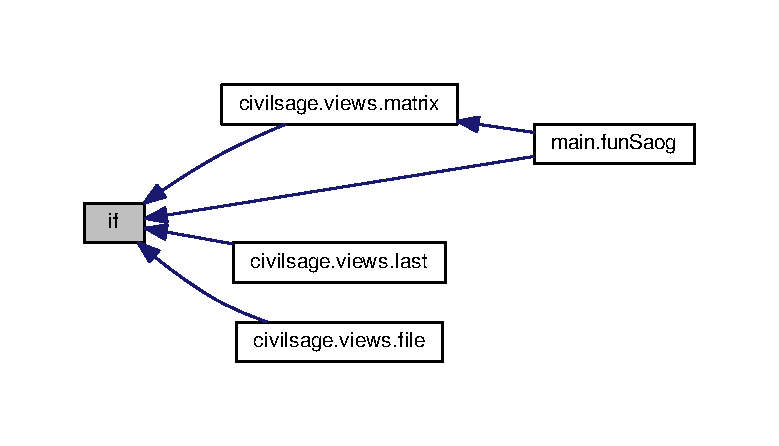
\includegraphics[width=350pt]{a00029_ac2d69f5011896c6ed4a54e0dd36f6334_icgraph}
\end{center}
\end{figure}


\hypertarget{a00029_a87cf461060832b8b68a7b48d9e371e4f}{}\index{bootstrap.\+min.\+js@{bootstrap.\+min.\+js}!if@{if}}
\index{if@{if}!bootstrap.\+min.\+js@{bootstrap.\+min.\+js}}
\subsubsection[{if(b[0]$<$ 2 \&\&b[1]$<$ 9\texttt{"|}\texttt{"|}1==b[0]\&\&9==b[1]\&\&b[2]$<$ 1) throw new Error(""Bootstrap\textquotesingle{}s Java\+Script requires j\+Query version 1.\+9.\+1 or higher"")\rcurly{}(j\+Query)}]{\setlength{\rightskip}{0pt plus 5cm}if (
\begin{DoxyParamCaption}
{}
\end{DoxyParamCaption}
)\hspace{0.3cm}{\ttfamily [new]}}\label{a00029_a87cf461060832b8b68a7b48d9e371e4f}


\subsection{Variable Documentation}
\hypertarget{a00029_ae8f6b400ed3390908c5cdeebed3a82b9}{}\index{bootstrap.\+min.\+js@{bootstrap.\+min.\+js}!a@{a}}
\index{a@{a}!bootstrap.\+min.\+js@{bootstrap.\+min.\+js}}
\subsubsection[{a}]{\setlength{\rightskip}{0pt plus 5cm}a {\bf fn} a {\bf fn} {\bf button} a {\bf fn} {\bf button} a \{\char`\"{}use strict\char`\"{}}\label{a00029_ae8f6b400ed3390908c5cdeebed3a82b9}


Definition at line 6 of file bootstrap.\+min.\+js.

\hypertarget{a00029_aaa41eef066735d697e7786ec86d52389}{}\index{bootstrap.\+min.\+js@{bootstrap.\+min.\+js}!alert@{alert}}
\index{alert@{alert}!bootstrap.\+min.\+js@{bootstrap.\+min.\+js}}
\subsubsection[{alert}]{\setlength{\rightskip}{0pt plus 5cm}{\bf a} {\bf fn} alert ={\bf b}}\label{a00029_aaa41eef066735d697e7786ec86d52389}


Definition at line 6 of file bootstrap.\+min.\+js.

\hypertarget{a00029_ac0431efac4d7c393d1e70b86115cb93f}{}\index{bootstrap.\+min.\+js@{bootstrap.\+min.\+js}!b@{b}}
\index{b@{b}!bootstrap.\+min.\+js@{bootstrap.\+min.\+js}}
\subsubsection[{b}]{\setlength{\rightskip}{0pt plus 5cm}function b =a.\+fn.\+jquery.\+split(\char`\"{} \char`\"{})\mbox{[}0\mbox{]}.split(\char`\"{}.\char`\"{})}\label{a00029_ac0431efac4d7c393d1e70b86115cb93f}


Definition at line 6 of file bootstrap.\+min.\+js.

\hypertarget{a00029_a55e170814e74f6c3db8ae9ea3ba9054f}{}\index{bootstrap.\+min.\+js@{bootstrap.\+min.\+js}!button@{button}}
\index{button@{button}!bootstrap.\+min.\+js@{bootstrap.\+min.\+js}}
\subsubsection[{button}]{\setlength{\rightskip}{0pt plus 5cm}{\bf a} {\bf fn} button ={\bf b}}\label{a00029_a55e170814e74f6c3db8ae9ea3ba9054f}


Definition at line 6 of file bootstrap.\+min.\+js.

\hypertarget{a00029_ad9d1ac02e33c4aed62ad517a7cb8b3fb}{}\index{bootstrap.\+min.\+js@{bootstrap.\+min.\+js}!c@{c}}
\index{c@{c}!bootstrap.\+min.\+js@{bootstrap.\+min.\+js}}
\subsubsection[{c}]{\setlength{\rightskip}{0pt plus 5cm}function c =\textquotesingle{}\mbox{[}data-\/dismiss=\char`\"{}alert\char`\"{}\mbox{]}\textquotesingle{}}\label{a00029_ad9d1ac02e33c4aed62ad517a7cb8b3fb}


Definition at line 6 of file bootstrap.\+min.\+js.

\hypertarget{a00029_a72fbb3628c3cc943ced8aad64247888c}{}\index{bootstrap.\+min.\+js@{bootstrap.\+min.\+js}!close@{close}}
\index{close@{close}!bootstrap.\+min.\+js@{bootstrap.\+min.\+js}}
\subsubsection[{close}]{\setlength{\rightskip}{0pt plus 5cm}{\bf d} {\bf d} {\bf d} prototype close =function({\bf b})\{function {\bf c}()\{g.\+detach().trigger(\char`\"{}closed.\+bs.\+alert\char`\"{}).remove()\}var {\bf e}={\bf a}(this),f=e.\+attr(\char`\"{}data-\/target\char`\"{});f$\vert$$\vert$(f=e.\+attr(\char`\"{}href\char`\"{}),f=f\&\&f.\+replace(/.$\ast$(?=\#\mbox{[}$^\wedge$\textbackslash{}s\mbox{]}$\ast$\$)/,\char`\"{}\char`\"{}));var g={\bf a}(f);{\bf b}\&\&b.\+prevent\+Default(),g.\+length$\vert$$\vert$(g=e.\+closest(\char`\"{}.alert\char`\"{})),g.\+trigger({\bf b}=a.\+Event(\char`\"{}close.\+bs.\+alert\char`\"{})),b.\+is\+Default\+Prevented()$\vert$$\vert$(g.\+remove\+Class(\char`\"{}in\char`\"{}),a.\+support.\+transition\&\&{\bf g.\+has\+Class}(\char`\"{}fade\char`\"{})?g.\+one(\char`\"{}bs\+Transition\+End\char`\"{},c).{\bf emulate\+Transition\+End}({\bf d.\+T\+R\+A\+N\+S\+I\+T\+I\+O\+N\+\_\+\+D\+U\+R\+A\+T\+I\+O\+N})\+:{\bf c}())\}}\label{a00029_a72fbb3628c3cc943ced8aad64247888c}


Definition at line 6 of file bootstrap.\+min.\+js.

\hypertarget{a00029_a0545907c609a48549a0cf5d4c692f851}{}\index{bootstrap.\+min.\+js@{bootstrap.\+min.\+js}!Constructor@{Constructor}}
\index{Constructor@{Constructor}!bootstrap.\+min.\+js@{bootstrap.\+min.\+js}}
\subsubsection[{Constructor}]{\setlength{\rightskip}{0pt plus 5cm}{\bf a} {\bf fn} {\bf a} {\bf fn} {\bf button} Constructor ={\bf d}}\label{a00029_a0545907c609a48549a0cf5d4c692f851}


Definition at line 6 of file bootstrap.\+min.\+js.

\hypertarget{a00029_aeb337d295abaddb5ec3cb34cc2e2bbc9}{}\index{bootstrap.\+min.\+js@{bootstrap.\+min.\+js}!d@{d}}
\index{d@{d}!bootstrap.\+min.\+js@{bootstrap.\+min.\+js}}
\subsubsection[{d}]{\setlength{\rightskip}{0pt plus 5cm}var d =function({\bf b})\{{\bf a}({\bf b}).on(\char`\"{}click\char`\"{},c,{\bf this.\+close})\}}\label{a00029_aeb337d295abaddb5ec3cb34cc2e2bbc9}


Definition at line 6 of file bootstrap.\+min.\+js.

\hypertarget{a00029_a6c1cf0be5e5383617ddc5efdfdc8c651}{}\index{bootstrap.\+min.\+js@{bootstrap.\+min.\+js}!D\+E\+F\+A\+U\+L\+T\+S@{D\+E\+F\+A\+U\+L\+T\+S}}
\index{D\+E\+F\+A\+U\+L\+T\+S@{D\+E\+F\+A\+U\+L\+T\+S}!bootstrap.\+min.\+js@{bootstrap.\+min.\+js}}
\subsubsection[{D\+E\+F\+A\+U\+L\+T\+S}]{\setlength{\rightskip}{0pt plus 5cm}{\bf c} {\bf c} D\+E\+F\+A\+U\+L\+T\+S =\{loading\+Text\+:\char`\"{}loading...\char`\"{}\}}\label{a00029_a6c1cf0be5e5383617ddc5efdfdc8c651}


Definition at line 6 of file bootstrap.\+min.\+js.

\hypertarget{a00029_ab5902775854a8b8440bcd25e0fe1c120}{}\index{bootstrap.\+min.\+js@{bootstrap.\+min.\+js}!e@{e}}
\index{e@{e}!bootstrap.\+min.\+js@{bootstrap.\+min.\+js}}
\subsubsection[{e}]{\setlength{\rightskip}{0pt plus 5cm}var e ={\bf a.\+fn.\+alert}}\label{a00029_ab5902775854a8b8440bcd25e0fe1c120}


Definition at line 6 of file bootstrap.\+min.\+js.

\hypertarget{a00029_a006fe6a2a254572b367123c6db401ff3}{}\index{bootstrap.\+min.\+js@{bootstrap.\+min.\+js}!emulate\+Transition\+End@{emulate\+Transition\+End}}
\index{emulate\+Transition\+End@{emulate\+Transition\+End}!bootstrap.\+min.\+js@{bootstrap.\+min.\+js}}
\subsubsection[{emulate\+Transition\+End}]{\setlength{\rightskip}{0pt plus 5cm}{\bf a} {\bf fn} emulate\+Transition\+End =function({\bf b})\{var {\bf c}=!1,{\bf d}=this;{\bf a}(this).one(\char`\"{}bs\+Transition\+End\char`\"{},function()\{{\bf c}=!0\});var {\bf e}=function()\{{\bf c}$\vert$$\vert${\bf a}({\bf d}).trigger(a.\+support.\+transition.\+end)\};return set\+Timeout({\bf e},{\bf b}),this\}}\label{a00029_a006fe6a2a254572b367123c6db401ff3}


Definition at line 6 of file bootstrap.\+min.\+js.

\hypertarget{a00029_ac26971afe341e4079ee34fceab395fc2}{}\index{bootstrap.\+min.\+js@{bootstrap.\+min.\+js}!no\+Conflict@{no\+Conflict}}
\index{no\+Conflict@{no\+Conflict}!bootstrap.\+min.\+js@{bootstrap.\+min.\+js}}
\subsubsection[{no\+Conflict}]{\setlength{\rightskip}{0pt plus 5cm}{\bf a} {\bf fn} {\bf a} {\bf fn} {\bf button} {\bf a} {\bf fn} {\bf button} no\+Conflict =function()\{return {\bf a.\+fn.\+alert}={\bf e},this\}}\label{a00029_ac26971afe341e4079ee34fceab395fc2}


Definition at line 6 of file bootstrap.\+min.\+js.

\hypertarget{a00029_a14f119ea3b5abc5536d590dfe1793c6e}{}\index{bootstrap.\+min.\+js@{bootstrap.\+min.\+js}!set\+State@{set\+State}}
\index{set\+State@{set\+State}!bootstrap.\+min.\+js@{bootstrap.\+min.\+js}}
\subsubsection[{set\+State}]{\setlength{\rightskip}{0pt plus 5cm}{\bf c} {\bf c} {\bf c} prototype set\+State =function({\bf b})\{var {\bf c}=\char`\"{}disabled\char`\"{},d=this.\$element,{\bf e}=d.\+is(\char`\"{}input\char`\"{})?\char`\"{}val\char`\"{}\+:\char`\"{}html\char`\"{},f=d.\+data();{\bf b}+=\char`\"{}Text\char`\"{},null==f.\+reset\+Text\&\&d.\+data(\char`\"{}reset\+Text\char`\"{},d\mbox{[}{\bf e}\mbox{]}()),set\+Timeout(a.\+proxy(function()\{{\bf d}\mbox{[}{\bf e}\mbox{]}(null==f\mbox{[}{\bf b}\mbox{]}?this.\+options\mbox{[}{\bf b}\mbox{]}\+:f\mbox{[}{\bf b}\mbox{]}),\char`\"{}loading\+Text\char`\"{}==b?(this.\+is\+Loading=!0,d.\+add\+Class({\bf c}).attr({\bf c},{\bf c}))\+:this.\+is\+Loading\&\&(this.\+is\+Loading=!1,d.\+remove\+Class({\bf c}).remove\+Attr({\bf c}))\},this),0)\}}\label{a00029_a14f119ea3b5abc5536d590dfe1793c6e}


Definition at line 6 of file bootstrap.\+min.\+js.

\hypertarget{a00029_aa8e797a9bda5e7e313be3518054164a3}{}\index{bootstrap.\+min.\+js@{bootstrap.\+min.\+js}!toggle@{toggle}}
\index{toggle@{toggle}!bootstrap.\+min.\+js@{bootstrap.\+min.\+js}}
\subsubsection[{toggle}]{\setlength{\rightskip}{0pt plus 5cm}{\bf c} {\bf c} {\bf c} prototype {\bf c} prototype toggle =function()\{var {\bf a}=!0,{\bf b}=this.\$element.\+closest(\textquotesingle{}\mbox{[}data-\/toggle=\char`\"{}buttons\char`\"{}\mbox{]}\textquotesingle{});if(b.\+length)\{var {\bf c}=this.\$element.\+find(\char`\"{}input\char`\"{});\char`\"{}radio\char`\"{}==c.\+prop(\char`\"{}type\char`\"{})?(c.\+prop(\char`\"{}checked\char`\"{})\&\&(a=!1),b.\+find(\char`\"{}.active\char`\"{}).remove\+Class(\char`\"{}active\char`\"{}),this.\$element.\+add\+Class(\char`\"{}active\char`\"{}))\+:\char`\"{}checkbox\char`\"{}==c.\+prop(\char`\"{}type\char`\"{})\&\&(c.\+prop(\char`\"{}checked\char`\"{})!==this.\$element.\+has\+Class(\char`\"{}active\char`\"{})\&\&(a=!1),this.\$element.\+toggle\+Class(\char`\"{}active\char`\"{})),c.\+prop(\char`\"{}checked\char`\"{},this.\$element.\+has\+Class(\char`\"{}active\char`\"{})),a\&\&c.\+trigger(\char`\"{}change\char`\"{})\}else this.\$element.\+attr(\char`\"{}aria-\/pressed\char`\"{},!this.\$element.\+has\+Class(\char`\"{}active\char`\"{})),this.\$element.\+toggle\+Class(\char`\"{}active\char`\"{})\}}\label{a00029_aa8e797a9bda5e7e313be3518054164a3}


Definition at line 6 of file bootstrap.\+min.\+js.

\hypertarget{a00029_ae4adb159aeacba734c34bd530baf92f6}{}\index{bootstrap.\+min.\+js@{bootstrap.\+min.\+js}!T\+R\+A\+N\+S\+I\+T\+I\+O\+N\+\_\+\+D\+U\+R\+A\+T\+I\+O\+N@{T\+R\+A\+N\+S\+I\+T\+I\+O\+N\+\_\+\+D\+U\+R\+A\+T\+I\+O\+N}}
\index{T\+R\+A\+N\+S\+I\+T\+I\+O\+N\+\_\+\+D\+U\+R\+A\+T\+I\+O\+N@{T\+R\+A\+N\+S\+I\+T\+I\+O\+N\+\_\+\+D\+U\+R\+A\+T\+I\+O\+N}!bootstrap.\+min.\+js@{bootstrap.\+min.\+js}}
\subsubsection[{T\+R\+A\+N\+S\+I\+T\+I\+O\+N\+\_\+\+D\+U\+R\+A\+T\+I\+O\+N}]{\setlength{\rightskip}{0pt plus 5cm}{\bf d} {\bf d} T\+R\+A\+N\+S\+I\+T\+I\+O\+N\+\_\+\+D\+U\+R\+A\+T\+I\+O\+N =150}\label{a00029_ae4adb159aeacba734c34bd530baf92f6}


Definition at line 6 of file bootstrap.\+min.\+js.

\hypertarget{a00029_a3635f2df5844f69204b70bf7b3983587}{}\index{bootstrap.\+min.\+js@{bootstrap.\+min.\+js}!V\+E\+R\+S\+I\+O\+N@{V\+E\+R\+S\+I\+O\+N}}
\index{V\+E\+R\+S\+I\+O\+N@{V\+E\+R\+S\+I\+O\+N}!bootstrap.\+min.\+js@{bootstrap.\+min.\+js}}
\subsubsection[{V\+E\+R\+S\+I\+O\+N}]{\setlength{\rightskip}{0pt plus 5cm}{\bf c} V\+E\+R\+S\+I\+O\+N =\char`\"{}3.\+3.\+5\char`\"{}}\label{a00029_a3635f2df5844f69204b70bf7b3983587}


Definition at line 6 of file bootstrap.\+min.\+js.


\hypertarget{a00030}{}\section{/home/amarjeet/projects/\+Civil\+Octave/sage/static/js/jquery.min.\+js File Reference}
\label{a00030}\index{/home/amarjeet/projects/\+Civil\+Octave/sage/static/js/jquery.\+min.\+js@{/home/amarjeet/projects/\+Civil\+Octave/sage/static/js/jquery.\+min.\+js}}
\subsection*{Functions}
\begin{DoxyCompactItemize}
\item 
\hyperlink{a00030_a43f0b96ea8ec44ca20ba86809a785614}{!function} (\hyperlink{a00029_a1f5870dcf487187f13d5fd328ed9e6e7}{a}, \hyperlink{a00029_a398bb8542498d1b14178b02b99df309b}{b})
\item 
m m m m \hyperlink{a00030_a18d9b499a0765bf2fe5f372ff2fc0236}{each} (\char`\"{}Boolean Number String Function Array Date Reg\+Exp Object Error\char`\"{}.split(\char`\"{} \char`\"{}), function(\hyperlink{a00029_a1f5870dcf487187f13d5fd328ed9e6e7}{a}, \hyperlink{a00029_a398bb8542498d1b14178b02b99df309b}{b})\{h\mbox{[}\char`\"{}\mbox{[}object \char`\"{}+b+\char`\"{}\mbox{]}\char`\"{}\mbox{]}=b.\+to\+Lower\+Case()\})
\item 
m m m \hyperlink{a00030_a30e1442d731d3fa211c24c68affccacd}{extend} (\{expando\+:\char`\"{}j\+Query\char`\"{}+(l+Math.\+random()).replace(/\textbackslash{}D/g,\char`\"{}\char`\"{}), is\+Ready\+:!0, error\+:function(\hyperlink{a00029_a1f5870dcf487187f13d5fd328ed9e6e7}{a})\{throw new Error(\hyperlink{a00029_a1f5870dcf487187f13d5fd328ed9e6e7}{a})\}, noop\+:function()\{\}, is\+Function\+:function(\hyperlink{a00029_a1f5870dcf487187f13d5fd328ed9e6e7}{a})\{return\char`\"{}function\char`\"{}===m.\+type(\hyperlink{a00029_a1f5870dcf487187f13d5fd328ed9e6e7}{a})\}, is\+Array\+:\+Array.\+is\+Array$\vert$$\vert$function(\hyperlink{a00029_a1f5870dcf487187f13d5fd328ed9e6e7}{a})\{return\char`\"{}array\char`\"{}===m.\+type(\hyperlink{a00029_a1f5870dcf487187f13d5fd328ed9e6e7}{a})\}, is\+Window\+:function(\hyperlink{a00029_a1f5870dcf487187f13d5fd328ed9e6e7}{a})\{return null!=\hyperlink{a00029_a1f5870dcf487187f13d5fd328ed9e6e7}{a} \&\&\hyperlink{a00029_a1f5870dcf487187f13d5fd328ed9e6e7}{a}==a.\+window\}, is\+Numeric\+:function(\hyperlink{a00029_a1f5870dcf487187f13d5fd328ed9e6e7}{a})\{return!m.\+is\+Array(\hyperlink{a00029_a1f5870dcf487187f13d5fd328ed9e6e7}{a})\&\&\hyperlink{a00029_a1f5870dcf487187f13d5fd328ed9e6e7}{a}-\/parse\+Float(\hyperlink{a00029_a1f5870dcf487187f13d5fd328ed9e6e7}{a})+1 $>$=0\}, is\+Empty\+Object\+:function(\hyperlink{a00029_a1f5870dcf487187f13d5fd328ed9e6e7}{a})\{var \hyperlink{a00029_a398bb8542498d1b14178b02b99df309b}{b};for(\hyperlink{a00029_a398bb8542498d1b14178b02b99df309b}{b} in \hyperlink{a00029_a1f5870dcf487187f13d5fd328ed9e6e7}{a}) return!1;return!0\}, is\+Plain\+Object\+:function(\hyperlink{a00029_a1f5870dcf487187f13d5fd328ed9e6e7}{a})\{var \hyperlink{a00029_a398bb8542498d1b14178b02b99df309b}{b};\hyperlink{a00029_a87cf461060832b8b68a7b48d9e371e4f}{if}(!\hyperlink{a00029_a1f5870dcf487187f13d5fd328ed9e6e7}{a}$\vert$$\vert$\char`\"{}object\char`\"{}!==m.\+type(\hyperlink{a00029_a1f5870dcf487187f13d5fd328ed9e6e7}{a})$\vert$$\vert$a.\+node\+Type$\vert$$\vert$m.\+is\+Window(\hyperlink{a00029_a1f5870dcf487187f13d5fd328ed9e6e7}{a})) return!1;try\{\hyperlink{a00029_a87cf461060832b8b68a7b48d9e371e4f}{if}(a.\+constructor \&\&!j.\+call(\hyperlink{a00029_a1f5870dcf487187f13d5fd328ed9e6e7}{a},\char`\"{}constructor\char`\"{})\&\&!j.\+call(a.\+constructor.\+prototype,\char`\"{}is\+Prototype\+Of\char`\"{})) return!1\}catch(\hyperlink{a00029_ad9d1ac02e33c4aed62ad517a7cb8b3fb}{c})\{return!1\}\hyperlink{a00029_a87cf461060832b8b68a7b48d9e371e4f}{if}(k.\+own\+Last) for(\hyperlink{a00029_a398bb8542498d1b14178b02b99df309b}{b} in \hyperlink{a00029_a1f5870dcf487187f13d5fd328ed9e6e7}{a}) return j.\+call(\hyperlink{a00029_a1f5870dcf487187f13d5fd328ed9e6e7}{a}, \hyperlink{a00029_a398bb8542498d1b14178b02b99df309b}{b});for(\hyperlink{a00029_a398bb8542498d1b14178b02b99df309b}{b} in \hyperlink{a00029_a1f5870dcf487187f13d5fd328ed9e6e7}{a});return void 0===\hyperlink{a00029_a398bb8542498d1b14178b02b99df309b}{b}$\vert$$\vert$j.\+call(\hyperlink{a00029_a1f5870dcf487187f13d5fd328ed9e6e7}{a}, \hyperlink{a00029_a398bb8542498d1b14178b02b99df309b}{b})\}, type\+:function(\hyperlink{a00029_a1f5870dcf487187f13d5fd328ed9e6e7}{a})\{return null==\hyperlink{a00029_a1f5870dcf487187f13d5fd328ed9e6e7}{a}?\hyperlink{a00029_a1f5870dcf487187f13d5fd328ed9e6e7}{a}+\char`\"{}\char`\"{}\+:\char`\"{}object\char`\"{}==typeof \hyperlink{a00029_a1f5870dcf487187f13d5fd328ed9e6e7}{a}$\vert$$\vert$\char`\"{}function\char`\"{}==typeof \hyperlink{a00029_a1f5870dcf487187f13d5fd328ed9e6e7}{a}?h\mbox{[}i.\+call(\hyperlink{a00029_a1f5870dcf487187f13d5fd328ed9e6e7}{a})\mbox{]}$\vert$$\vert$\char`\"{}object\char`\"{}\+:typeof \hyperlink{a00029_a1f5870dcf487187f13d5fd328ed9e6e7}{a}\}, global\+Eval\+:function(\hyperlink{a00029_a398bb8542498d1b14178b02b99df309b}{b})\{\hyperlink{a00029_a398bb8542498d1b14178b02b99df309b}{b} \&\&m.\+trim(\hyperlink{a00029_a398bb8542498d1b14178b02b99df309b}{b})\&\&(a.\+exec\+Script$\vert$$\vert$function(\hyperlink{a00029_a398bb8542498d1b14178b02b99df309b}{b})\{a.\+eval.\+call(\hyperlink{a00029_a1f5870dcf487187f13d5fd328ed9e6e7}{a}, \hyperlink{a00029_a398bb8542498d1b14178b02b99df309b}{b})\})(\hyperlink{a00029_a398bb8542498d1b14178b02b99df309b}{b})\}, camel\+Case\+:function(\hyperlink{a00029_a1f5870dcf487187f13d5fd328ed9e6e7}{a})\{return a.\+replace(o,\char`\"{}ms-\/\char`\"{}).replace(p, q)\}, node\+Name\+:function(\hyperlink{a00029_a1f5870dcf487187f13d5fd328ed9e6e7}{a}, \hyperlink{a00029_a398bb8542498d1b14178b02b99df309b}{b})\{return a.\+node\+Name \&\&a.\+node\+Name.\+to\+Lower\+Case()===b.\+to\+Lower\+Case()\}, each\+:function(\hyperlink{a00029_a1f5870dcf487187f13d5fd328ed9e6e7}{a}, \hyperlink{a00029_a398bb8542498d1b14178b02b99df309b}{b}, \hyperlink{a00029_ad9d1ac02e33c4aed62ad517a7cb8b3fb}{c})\{var \hyperlink{a00029_aeb337d295abaddb5ec3cb34cc2e2bbc9}{d}, \hyperlink{a00029_ab5902775854a8b8440bcd25e0fe1c120}{e}=0, f=a.\+length, g=\hyperlink{a00030_a96f65b399314d93896076ceb474b6b9b}{r}(\hyperlink{a00029_a1f5870dcf487187f13d5fd328ed9e6e7}{a});\hyperlink{a00029_a87cf461060832b8b68a7b48d9e371e4f}{if}(\hyperlink{a00029_ad9d1ac02e33c4aed62ad517a7cb8b3fb}{c})\{\hyperlink{a00029_a87cf461060832b8b68a7b48d9e371e4f}{if}(g)\{for(;f $>$\hyperlink{a00029_ab5902775854a8b8440bcd25e0fe1c120}{e};\hyperlink{a00029_ab5902775854a8b8440bcd25e0fe1c120}{e}++) \hyperlink{a00029_a87cf461060832b8b68a7b48d9e371e4f}{if}(\hyperlink{a00029_aeb337d295abaddb5ec3cb34cc2e2bbc9}{d}=b.\+apply(\hyperlink{a00029_a1f5870dcf487187f13d5fd328ed9e6e7}{a}\mbox{[}\hyperlink{a00029_ab5902775854a8b8440bcd25e0fe1c120}{e}\mbox{]}, \hyperlink{a00029_ad9d1ac02e33c4aed62ad517a7cb8b3fb}{c}), \hyperlink{a00029_aeb337d295abaddb5ec3cb34cc2e2bbc9}{d}===!1) break\}else for(\hyperlink{a00029_ab5902775854a8b8440bcd25e0fe1c120}{e} in \hyperlink{a00029_a1f5870dcf487187f13d5fd328ed9e6e7}{a}) \hyperlink{a00029_a87cf461060832b8b68a7b48d9e371e4f}{if}(\hyperlink{a00029_aeb337d295abaddb5ec3cb34cc2e2bbc9}{d}=b.\+apply(\hyperlink{a00029_a1f5870dcf487187f13d5fd328ed9e6e7}{a}\mbox{[}\hyperlink{a00029_ab5902775854a8b8440bcd25e0fe1c120}{e}\mbox{]}, \hyperlink{a00029_ad9d1ac02e33c4aed62ad517a7cb8b3fb}{c}), \hyperlink{a00029_aeb337d295abaddb5ec3cb34cc2e2bbc9}{d}===!1) break\}else \hyperlink{a00029_a87cf461060832b8b68a7b48d9e371e4f}{if}(g)\{for(;f $>$\hyperlink{a00029_ab5902775854a8b8440bcd25e0fe1c120}{e};\hyperlink{a00029_ab5902775854a8b8440bcd25e0fe1c120}{e}++) \hyperlink{a00029_a87cf461060832b8b68a7b48d9e371e4f}{if}(\hyperlink{a00029_aeb337d295abaddb5ec3cb34cc2e2bbc9}{d}=b.\+call(\hyperlink{a00029_a1f5870dcf487187f13d5fd328ed9e6e7}{a}\mbox{[}\hyperlink{a00029_ab5902775854a8b8440bcd25e0fe1c120}{e}\mbox{]}, \hyperlink{a00029_ab5902775854a8b8440bcd25e0fe1c120}{e}, \hyperlink{a00029_a1f5870dcf487187f13d5fd328ed9e6e7}{a}\mbox{[}\hyperlink{a00029_ab5902775854a8b8440bcd25e0fe1c120}{e}\mbox{]}), \hyperlink{a00029_aeb337d295abaddb5ec3cb34cc2e2bbc9}{d}===!1) break\}else for(\hyperlink{a00029_ab5902775854a8b8440bcd25e0fe1c120}{e} in \hyperlink{a00029_a1f5870dcf487187f13d5fd328ed9e6e7}{a}) \hyperlink{a00029_a87cf461060832b8b68a7b48d9e371e4f}{if}(\hyperlink{a00029_aeb337d295abaddb5ec3cb34cc2e2bbc9}{d}=b.\+call(\hyperlink{a00029_a1f5870dcf487187f13d5fd328ed9e6e7}{a}\mbox{[}\hyperlink{a00029_ab5902775854a8b8440bcd25e0fe1c120}{e}\mbox{]}, \hyperlink{a00029_ab5902775854a8b8440bcd25e0fe1c120}{e}, \hyperlink{a00029_a1f5870dcf487187f13d5fd328ed9e6e7}{a}\mbox{[}\hyperlink{a00029_ab5902775854a8b8440bcd25e0fe1c120}{e}\mbox{]}), \hyperlink{a00029_aeb337d295abaddb5ec3cb34cc2e2bbc9}{d}===!1) break;return \hyperlink{a00029_a1f5870dcf487187f13d5fd328ed9e6e7}{a}\}, trim\+:function(\hyperlink{a00029_a1f5870dcf487187f13d5fd328ed9e6e7}{a})\{return null==\hyperlink{a00029_a1f5870dcf487187f13d5fd328ed9e6e7}{a}?\char`\"{}\char`\"{}\+:(\hyperlink{a00029_a1f5870dcf487187f13d5fd328ed9e6e7}{a}+\char`\"{}\char`\"{}).replace(n,\char`\"{}\char`\"{})\}, make\+Array\+:function(\hyperlink{a00029_a1f5870dcf487187f13d5fd328ed9e6e7}{a}, \hyperlink{a00029_a398bb8542498d1b14178b02b99df309b}{b})\{var \hyperlink{a00029_ad9d1ac02e33c4aed62ad517a7cb8b3fb}{c}=\hyperlink{a00029_a398bb8542498d1b14178b02b99df309b}{b}$\vert$$\vert$\mbox{[}$\,$\mbox{]};return null!=\hyperlink{a00029_a1f5870dcf487187f13d5fd328ed9e6e7}{a} \&\&(\hyperlink{a00030_a96f65b399314d93896076ceb474b6b9b}{r}(Object(\hyperlink{a00029_a1f5870dcf487187f13d5fd328ed9e6e7}{a}))?m.\+merge(\hyperlink{a00029_ad9d1ac02e33c4aed62ad517a7cb8b3fb}{c},\char`\"{}string\char`\"{}==typeof \hyperlink{a00029_a1f5870dcf487187f13d5fd328ed9e6e7}{a}?\mbox{[}\hyperlink{a00029_a1f5870dcf487187f13d5fd328ed9e6e7}{a}\mbox{]}\+:\hyperlink{a00029_a1f5870dcf487187f13d5fd328ed9e6e7}{a})\+:f.\+call(\hyperlink{a00029_ad9d1ac02e33c4aed62ad517a7cb8b3fb}{c}, \hyperlink{a00029_a1f5870dcf487187f13d5fd328ed9e6e7}{a})), \hyperlink{a00029_ad9d1ac02e33c4aed62ad517a7cb8b3fb}{c}\}, in\+Array\+:function(\hyperlink{a00029_a1f5870dcf487187f13d5fd328ed9e6e7}{a}, \hyperlink{a00029_a398bb8542498d1b14178b02b99df309b}{b}, \hyperlink{a00029_ad9d1ac02e33c4aed62ad517a7cb8b3fb}{c})\{var \hyperlink{a00029_aeb337d295abaddb5ec3cb34cc2e2bbc9}{d};\hyperlink{a00029_a87cf461060832b8b68a7b48d9e371e4f}{if}(\hyperlink{a00029_a398bb8542498d1b14178b02b99df309b}{b})\{\hyperlink{a00029_a87cf461060832b8b68a7b48d9e371e4f}{if}(g) return g.\+call(\hyperlink{a00029_a398bb8542498d1b14178b02b99df309b}{b}, \hyperlink{a00029_a1f5870dcf487187f13d5fd328ed9e6e7}{a}, \hyperlink{a00029_ad9d1ac02e33c4aed62ad517a7cb8b3fb}{c});for(\hyperlink{a00029_aeb337d295abaddb5ec3cb34cc2e2bbc9}{d}=b.\+length, \hyperlink{a00029_ad9d1ac02e33c4aed62ad517a7cb8b3fb}{c}=\hyperlink{a00029_ad9d1ac02e33c4aed62ad517a7cb8b3fb}{c}?0 $>$\hyperlink{a00029_ad9d1ac02e33c4aed62ad517a7cb8b3fb}{c}?Math.\+max(0, \hyperlink{a00029_aeb337d295abaddb5ec3cb34cc2e2bbc9}{d}+\hyperlink{a00029_ad9d1ac02e33c4aed62ad517a7cb8b3fb}{c})\+:c\+:0;\hyperlink{a00029_aeb337d295abaddb5ec3cb34cc2e2bbc9}{d} $>$\hyperlink{a00029_ad9d1ac02e33c4aed62ad517a7cb8b3fb}{c};\hyperlink{a00029_ad9d1ac02e33c4aed62ad517a7cb8b3fb}{c}++) \hyperlink{a00029_a87cf461060832b8b68a7b48d9e371e4f}{if}(\hyperlink{a00029_ad9d1ac02e33c4aed62ad517a7cb8b3fb}{c} in \hyperlink{a00029_a398bb8542498d1b14178b02b99df309b}{b} \&\&\hyperlink{a00029_a398bb8542498d1b14178b02b99df309b}{b}\mbox{[}\hyperlink{a00029_ad9d1ac02e33c4aed62ad517a7cb8b3fb}{c}\mbox{]}===\hyperlink{a00029_a1f5870dcf487187f13d5fd328ed9e6e7}{a}) return \hyperlink{a00029_ad9d1ac02e33c4aed62ad517a7cb8b3fb}{c}\}return-\/1\}, merge\+:function(\hyperlink{a00029_a1f5870dcf487187f13d5fd328ed9e6e7}{a}, \hyperlink{a00029_a398bb8542498d1b14178b02b99df309b}{b})\{var \hyperlink{a00029_ad9d1ac02e33c4aed62ad517a7cb8b3fb}{c}=+b.\+length, \hyperlink{a00029_aeb337d295abaddb5ec3cb34cc2e2bbc9}{d}=0, \hyperlink{a00029_ab5902775854a8b8440bcd25e0fe1c120}{e}=a.\+length;while(\hyperlink{a00029_ad9d1ac02e33c4aed62ad517a7cb8b3fb}{c} $>$\hyperlink{a00029_aeb337d295abaddb5ec3cb34cc2e2bbc9}{d}) \hyperlink{a00029_a1f5870dcf487187f13d5fd328ed9e6e7}{a}\mbox{[}\hyperlink{a00029_ab5902775854a8b8440bcd25e0fe1c120}{e}++\mbox{]}=\hyperlink{a00029_a398bb8542498d1b14178b02b99df309b}{b}\mbox{[}\hyperlink{a00029_aeb337d295abaddb5ec3cb34cc2e2bbc9}{d}++\mbox{]};\hyperlink{a00029_a87cf461060832b8b68a7b48d9e371e4f}{if}(c!==\hyperlink{a00029_ad9d1ac02e33c4aed62ad517a7cb8b3fb}{c}) while(void 0!==\hyperlink{a00029_a398bb8542498d1b14178b02b99df309b}{b}\mbox{[}\hyperlink{a00029_aeb337d295abaddb5ec3cb34cc2e2bbc9}{d}\mbox{]}) \hyperlink{a00029_a1f5870dcf487187f13d5fd328ed9e6e7}{a}\mbox{[}\hyperlink{a00029_ab5902775854a8b8440bcd25e0fe1c120}{e}++\mbox{]}=\hyperlink{a00029_a398bb8542498d1b14178b02b99df309b}{b}\mbox{[}\hyperlink{a00029_aeb337d295abaddb5ec3cb34cc2e2bbc9}{d}++\mbox{]};return a.\+length=\hyperlink{a00029_ab5902775854a8b8440bcd25e0fe1c120}{e}, \hyperlink{a00029_a1f5870dcf487187f13d5fd328ed9e6e7}{a}\}, grep\+:function(\hyperlink{a00029_a1f5870dcf487187f13d5fd328ed9e6e7}{a}, \hyperlink{a00029_a398bb8542498d1b14178b02b99df309b}{b}, \hyperlink{a00029_ad9d1ac02e33c4aed62ad517a7cb8b3fb}{c})\{for(var \hyperlink{a00029_aeb337d295abaddb5ec3cb34cc2e2bbc9}{d}, \hyperlink{a00029_ab5902775854a8b8440bcd25e0fe1c120}{e}=\mbox{[}$\,$\mbox{]}, f=0, g=a.\+length, h=!\hyperlink{a00029_ad9d1ac02e33c4aed62ad517a7cb8b3fb}{c};g $>$f;f++) \hyperlink{a00029_aeb337d295abaddb5ec3cb34cc2e2bbc9}{d}=!\hyperlink{a00029_a398bb8542498d1b14178b02b99df309b}{b}(\hyperlink{a00029_a1f5870dcf487187f13d5fd328ed9e6e7}{a}\mbox{[}f\mbox{]}, f), d!==h \&\&e.\+push(\hyperlink{a00029_a1f5870dcf487187f13d5fd328ed9e6e7}{a}\mbox{[}f\mbox{]});return \hyperlink{a00029_ab5902775854a8b8440bcd25e0fe1c120}{e}\}, map\+:function(\hyperlink{a00029_a1f5870dcf487187f13d5fd328ed9e6e7}{a}, \hyperlink{a00029_a398bb8542498d1b14178b02b99df309b}{b}, \hyperlink{a00029_ad9d1ac02e33c4aed62ad517a7cb8b3fb}{c})\{var \hyperlink{a00029_aeb337d295abaddb5ec3cb34cc2e2bbc9}{d}, f=0, g=a.\+length, h=\hyperlink{a00030_a96f65b399314d93896076ceb474b6b9b}{r}(\hyperlink{a00029_a1f5870dcf487187f13d5fd328ed9e6e7}{a}), \hyperlink{a00008_a6dbbc96f4222af2f6c18c8e60f41726b}{i}=\mbox{[}$\,$\mbox{]};\hyperlink{a00029_a87cf461060832b8b68a7b48d9e371e4f}{if}(h) for(;g $>$f;f++) \hyperlink{a00029_aeb337d295abaddb5ec3cb34cc2e2bbc9}{d}=\hyperlink{a00029_a398bb8542498d1b14178b02b99df309b}{b}(\hyperlink{a00029_a1f5870dcf487187f13d5fd328ed9e6e7}{a}\mbox{[}f\mbox{]}, f, \hyperlink{a00029_ad9d1ac02e33c4aed62ad517a7cb8b3fb}{c}), null!=\hyperlink{a00029_aeb337d295abaddb5ec3cb34cc2e2bbc9}{d} \&\&i.\+push(\hyperlink{a00029_aeb337d295abaddb5ec3cb34cc2e2bbc9}{d});else for(f in \hyperlink{a00029_a1f5870dcf487187f13d5fd328ed9e6e7}{a}) \hyperlink{a00029_aeb337d295abaddb5ec3cb34cc2e2bbc9}{d}=\hyperlink{a00029_a398bb8542498d1b14178b02b99df309b}{b}(\hyperlink{a00029_a1f5870dcf487187f13d5fd328ed9e6e7}{a}\mbox{[}f\mbox{]}, f, \hyperlink{a00029_ad9d1ac02e33c4aed62ad517a7cb8b3fb}{c}), null!=\hyperlink{a00029_aeb337d295abaddb5ec3cb34cc2e2bbc9}{d} \&\&i.\+push(\hyperlink{a00029_aeb337d295abaddb5ec3cb34cc2e2bbc9}{d});return e.\+apply(\mbox{[}$\,$\mbox{]}, \hyperlink{a00008_a6dbbc96f4222af2f6c18c8e60f41726b}{i})\}, guid\+:1, proxy\+:function(\hyperlink{a00029_a1f5870dcf487187f13d5fd328ed9e6e7}{a}, \hyperlink{a00029_a398bb8542498d1b14178b02b99df309b}{b})\{var \hyperlink{a00029_ad9d1ac02e33c4aed62ad517a7cb8b3fb}{c}, \hyperlink{a00029_ab5902775854a8b8440bcd25e0fe1c120}{e}, f;return\char`\"{}string\char`\"{}==typeof \hyperlink{a00029_a398bb8542498d1b14178b02b99df309b}{b} \&\&(f=\hyperlink{a00029_a1f5870dcf487187f13d5fd328ed9e6e7}{a}\mbox{[}\hyperlink{a00029_a398bb8542498d1b14178b02b99df309b}{b}\mbox{]}, \hyperlink{a00029_a398bb8542498d1b14178b02b99df309b}{b}=\hyperlink{a00029_a1f5870dcf487187f13d5fd328ed9e6e7}{a}, \hyperlink{a00029_a1f5870dcf487187f13d5fd328ed9e6e7}{a}=f), m.\+is\+Function(\hyperlink{a00029_a1f5870dcf487187f13d5fd328ed9e6e7}{a})?(\hyperlink{a00029_ad9d1ac02e33c4aed62ad517a7cb8b3fb}{c}=d.\+call(arguments, 2), \hyperlink{a00029_ab5902775854a8b8440bcd25e0fe1c120}{e}=function()\{return a.\+apply(\hyperlink{a00029_a398bb8542498d1b14178b02b99df309b}{b}$\vert$$\vert$this, c.\+concat(d.\+call(arguments)))\}, e.\+guid=a.\+guid=a.\+guid$\vert$$\vert$m.\+guid++, \hyperlink{a00029_ab5902775854a8b8440bcd25e0fe1c120}{e})\+:void 0\}, now\+:function()\{return+new Date\}, support\+:k\})
\item 
function \hyperlink{a00030_a96f65b399314d93896076ceb474b6b9b}{r} (\hyperlink{a00029_a1f5870dcf487187f13d5fd328ed9e6e7}{a})
\end{DoxyCompactItemize}
\subsection*{Variables}
\begin{DoxyCompactItemize}
\item 
function \hyperlink{a00030_aa4d4888597588a84fd5b1184d00c91f3}{a}
\item 
function \hyperlink{a00030_ac0431efac4d7c393d1e70b86115cb93f}{b} \{var \hyperlink{a00029_ad9d1ac02e33c4aed62ad517a7cb8b3fb}{c}=\mbox{[}$\,$\mbox{]},\hyperlink{a00029_aeb337d295abaddb5ec3cb34cc2e2bbc9}{d}=c.\+slice,\hyperlink{a00029_ab5902775854a8b8440bcd25e0fe1c120}{e}=c.\+concat,f=c.\+push,g=c.\+index\+Of,h=\{\},\hyperlink{a00008_a6dbbc96f4222af2f6c18c8e60f41726b}{i}=h.\+to\+String,\hyperlink{a00008_ac86694252f8dfdb19aaeadc4b7c342c6}{j}=h.\+has\+Own\+Property,k=\{\},l=\char`\"{}1.\+11.\+3\char`\"{},m=function(\hyperlink{a00029_a1f5870dcf487187f13d5fd328ed9e6e7}{a},b)\{return new m.\+fn.\+init(\hyperlink{a00029_a1f5870dcf487187f13d5fd328ed9e6e7}{a},b)\},n=/$^\wedge$\mbox{[}\textbackslash{}s\textbackslash{}u\+F\+E\+F\+F\textbackslash{}x\+A0\mbox{]}+$\vert$\mbox{[}\textbackslash{}s\textbackslash{}u\+F\+E\+F\+F\textbackslash{}x\+A0\mbox{]}+\$/g,o=/$^\wedge$-\/ms-\//,p=/-\/(\mbox{[}\textbackslash{}da-\/z\mbox{]})/gi,q=function(\hyperlink{a00029_a1f5870dcf487187f13d5fd328ed9e6e7}{a},b)\{return b.\+to\+Upper\+Case()\}
\item 
m m \hyperlink{a00030_a167947be5252c14d5389d8a01a8c8545}{extend} =m.\+fn.\+extend=function()\{var \hyperlink{a00029_a1f5870dcf487187f13d5fd328ed9e6e7}{a},\hyperlink{a00029_a398bb8542498d1b14178b02b99df309b}{b},\hyperlink{a00029_ad9d1ac02e33c4aed62ad517a7cb8b3fb}{c},\hyperlink{a00029_aeb337d295abaddb5ec3cb34cc2e2bbc9}{d},\hyperlink{a00029_ab5902775854a8b8440bcd25e0fe1c120}{e},f,g=arguments\mbox{[}0\mbox{]}$\vert$$\vert$\{\},h=1,\hyperlink{a00008_a6dbbc96f4222af2f6c18c8e60f41726b}{i}=arguments.\+length,\hyperlink{a00008_ac86694252f8dfdb19aaeadc4b7c342c6}{j}=!1;for(\char`\"{}boolean\char`\"{}==typeof g\&\&(\hyperlink{a00008_ac86694252f8dfdb19aaeadc4b7c342c6}{j}=g,g=arguments\mbox{[}h\mbox{]}$\vert$$\vert$\{\},h++),\char`\"{}object\char`\"{}==typeof g$\vert$$\vert$m.\+is\+Function(g)$\vert$$\vert$(g=\{\}),h===\hyperlink{a00008_a6dbbc96f4222af2f6c18c8e60f41726b}{i}\&\&(g=this,h-\/-\/);\hyperlink{a00008_a6dbbc96f4222af2f6c18c8e60f41726b}{i}$>$h;h++)\hyperlink{a00029_a87cf461060832b8b68a7b48d9e371e4f}{if}(null!=(\hyperlink{a00029_ab5902775854a8b8440bcd25e0fe1c120}{e}=arguments\mbox{[}h\mbox{]}))for(\hyperlink{a00029_aeb337d295abaddb5ec3cb34cc2e2bbc9}{d} in \hyperlink{a00029_ab5902775854a8b8440bcd25e0fe1c120}{e})\hyperlink{a00029_a1f5870dcf487187f13d5fd328ed9e6e7}{a}=g\mbox{[}\hyperlink{a00029_aeb337d295abaddb5ec3cb34cc2e2bbc9}{d}\mbox{]},\hyperlink{a00029_ad9d1ac02e33c4aed62ad517a7cb8b3fb}{c}=\hyperlink{a00029_ab5902775854a8b8440bcd25e0fe1c120}{e}\mbox{[}\hyperlink{a00029_aeb337d295abaddb5ec3cb34cc2e2bbc9}{d}\mbox{]},g!==\hyperlink{a00029_ad9d1ac02e33c4aed62ad517a7cb8b3fb}{c}\&\&(\hyperlink{a00008_ac86694252f8dfdb19aaeadc4b7c342c6}{j}\&\&\hyperlink{a00029_ad9d1ac02e33c4aed62ad517a7cb8b3fb}{c}\&\&(m.\+is\+Plain\+Object(\hyperlink{a00029_ad9d1ac02e33c4aed62ad517a7cb8b3fb}{c})$\vert$$\vert$(\hyperlink{a00029_a398bb8542498d1b14178b02b99df309b}{b}=m.\+is\+Array(\hyperlink{a00029_ad9d1ac02e33c4aed62ad517a7cb8b3fb}{c})))?(\hyperlink{a00029_a398bb8542498d1b14178b02b99df309b}{b}?(\hyperlink{a00029_a398bb8542498d1b14178b02b99df309b}{b}=!1,f=\hyperlink{a00029_a1f5870dcf487187f13d5fd328ed9e6e7}{a}\&\&m.\+is\+Array(\hyperlink{a00029_a1f5870dcf487187f13d5fd328ed9e6e7}{a})?a\+:\mbox{[}$\,$\mbox{]})\+:f=\hyperlink{a00029_a1f5870dcf487187f13d5fd328ed9e6e7}{a}\&\&m.\+is\+Plain\+Object(\hyperlink{a00029_a1f5870dcf487187f13d5fd328ed9e6e7}{a})?a\+:\{\},g\mbox{[}\hyperlink{a00029_aeb337d295abaddb5ec3cb34cc2e2bbc9}{d}\mbox{]}=m.\+extend(\hyperlink{a00008_ac86694252f8dfdb19aaeadc4b7c342c6}{j},f,\hyperlink{a00029_ad9d1ac02e33c4aed62ad517a7cb8b3fb}{c}))\+:void 0!==\hyperlink{a00029_ad9d1ac02e33c4aed62ad517a7cb8b3fb}{c}\&\&(g\mbox{[}\hyperlink{a00029_aeb337d295abaddb5ec3cb34cc2e2bbc9}{d}\mbox{]}=\hyperlink{a00029_ad9d1ac02e33c4aed62ad517a7cb8b3fb}{c}));return g\}
\item 
m \hyperlink{a00030_ab2836ee14921cbd6e34ea91a9a99ad66}{fn} =m.\+prototype=\{jquery\+:l,constructor\+:m,selector\+:\char`\"{}\char`\"{},length\+:0,to\+Array\+:function()\{return d.\+call(this)\},get\+:function(\hyperlink{a00029_a1f5870dcf487187f13d5fd328ed9e6e7}{a})\{return null!=\hyperlink{a00029_a1f5870dcf487187f13d5fd328ed9e6e7}{a}?0$>$\hyperlink{a00029_a1f5870dcf487187f13d5fd328ed9e6e7}{a}?this\mbox{[}\hyperlink{a00029_a1f5870dcf487187f13d5fd328ed9e6e7}{a}+this.\+length\mbox{]}\+:this\mbox{[}\hyperlink{a00029_a1f5870dcf487187f13d5fd328ed9e6e7}{a}\mbox{]}\+:d.\+call(this)\},push\+Stack\+:function(\hyperlink{a00029_a1f5870dcf487187f13d5fd328ed9e6e7}{a})\{var \hyperlink{a00029_a398bb8542498d1b14178b02b99df309b}{b}=m.\+merge(this.\+constructor(),\hyperlink{a00029_a1f5870dcf487187f13d5fd328ed9e6e7}{a});return b.\+prev\+Object=this,b.\+context=this.\+context,\hyperlink{a00029_a398bb8542498d1b14178b02b99df309b}{b}\},each\+:function(\hyperlink{a00029_a1f5870dcf487187f13d5fd328ed9e6e7}{a},\hyperlink{a00029_a398bb8542498d1b14178b02b99df309b}{b})\{return \hyperlink{a00030_a18d9b499a0765bf2fe5f372ff2fc0236}{m.\+each}(this,\hyperlink{a00029_a1f5870dcf487187f13d5fd328ed9e6e7}{a},\hyperlink{a00029_a398bb8542498d1b14178b02b99df309b}{b})\},map\+:function(\hyperlink{a00029_a1f5870dcf487187f13d5fd328ed9e6e7}{a})\{return this.\+push\+Stack(m.\+map(this,function(\hyperlink{a00029_a398bb8542498d1b14178b02b99df309b}{b},\hyperlink{a00029_ad9d1ac02e33c4aed62ad517a7cb8b3fb}{c})\{return a.\+call(\hyperlink{a00029_a398bb8542498d1b14178b02b99df309b}{b},\hyperlink{a00029_ad9d1ac02e33c4aed62ad517a7cb8b3fb}{c},\hyperlink{a00029_a398bb8542498d1b14178b02b99df309b}{b})\}))\},slice\+:function()\{return this.\+push\+Stack(d.\+apply(this,arguments))\},first\+:function()\{return this.\+eq(0)\},last\+:function()\{return this.\+eq(-\/1)\},eq\+:function(\hyperlink{a00029_a1f5870dcf487187f13d5fd328ed9e6e7}{a})\{var \hyperlink{a00029_a398bb8542498d1b14178b02b99df309b}{b}=this.\+length,\hyperlink{a00029_ad9d1ac02e33c4aed62ad517a7cb8b3fb}{c}=+\hyperlink{a00029_a1f5870dcf487187f13d5fd328ed9e6e7}{a}+(0$>$\hyperlink{a00029_a1f5870dcf487187f13d5fd328ed9e6e7}{a}?b\+:0);return this.\+push\+Stack(\hyperlink{a00029_ad9d1ac02e33c4aed62ad517a7cb8b3fb}{c}$>$=0\&\&\hyperlink{a00029_a398bb8542498d1b14178b02b99df309b}{b}$>$\hyperlink{a00029_ad9d1ac02e33c4aed62ad517a7cb8b3fb}{c}?\mbox{[}this\mbox{[}\hyperlink{a00029_ad9d1ac02e33c4aed62ad517a7cb8b3fb}{c}\mbox{]}\mbox{]}\+:\mbox{[}$\,$\mbox{]})\},end\+:function()\{return this.\+prev\+Object$\vert$$\vert$this.\+constructor(null)\},push\+:f,sort\+:c.\+sort,splice\+:c.\+splice\}
\item 
\hyperlink{a00030_ae21cc36bf0d65014c717a481a3f8a468}{undefined} =typeof window?window\+:this
\end{DoxyCompactItemize}


\subsection{Function Documentation}
\hypertarget{a00030_a43f0b96ea8ec44ca20ba86809a785614}{}\index{jquery.\+min.\+js@{jquery.\+min.\+js}!"!function@{"!function}}
\index{"!function@{"!function}!jquery.\+min.\+js@{jquery.\+min.\+js}}
\subsubsection[{"!function(a, b)}]{\setlength{\rightskip}{0pt plus 5cm}!function (
\begin{DoxyParamCaption}
\item[{}]{a, }
\item[{}]{b}
\end{DoxyParamCaption}
)}\label{a00030_a43f0b96ea8ec44ca20ba86809a785614}
j\+Query v1.\+11.\+3 $\vert$ (c) 2005, 2015 j\+Query Foundation, Inc. $\vert$ jquery.\+org/license 

Definition at line 2 of file jquery.\+min.\+js.


\begin{DoxyCode}
2 \{\textcolor{stringliteral}{"object"}==typeof module&&\textcolor{stringliteral}{"object"}==typeof module.exports?module.exports=\hyperlink{a00030_aa4d4888597588a84fd5b1184d00c91f3}{a}.document?
      \hyperlink{a00030_ac0431efac4d7c393d1e70b86115cb93f}{b}(\hyperlink{a00030_aa4d4888597588a84fd5b1184d00c91f3}{a},!0):function(\hyperlink{a00030_aa4d4888597588a84fd5b1184d00c91f3}{a})\{\textcolor{keywordflow}{if}(!\hyperlink{a00030_aa4d4888597588a84fd5b1184d00c91f3}{a}.document)\textcolor{keywordflow}{throw} \textcolor{keyword}{new} Error(\textcolor{stringliteral}{"jQuery requires a window with a document"});\textcolor{keywordflow}{return} 
      \hyperlink{a00030_ac0431efac4d7c393d1e70b86115cb93f}{b}(\hyperlink{a00030_aa4d4888597588a84fd5b1184d00c91f3}{a})\}:\hyperlink{a00030_ac0431efac4d7c393d1e70b86115cb93f}{b}(\hyperlink{a00030_aa4d4888597588a84fd5b1184d00c91f3}{a})\}(\textcolor{stringliteral}{"undefined"}!=typeof window?window:\textcolor{keyword}{this},\textcolor{keyword}{function}(\hyperlink{a00030_aa4d4888597588a84fd5b1184d00c91f3}{a},\hyperlink{a00030_ac0431efac4d7c393d1e70b86115cb93f}{b})\{var \hyperlink{a00029_ad9d1ac02e33c4aed62ad517a7cb8b3fb}{c}=[],
      \hyperlink{a00029_aeb337d295abaddb5ec3cb34cc2e2bbc9}{d}=c.slice,\hyperlink{a00029_ab5902775854a8b8440bcd25e0fe1c120}{e}=c.concat,f=c.push,g=c.indexOf,h=\{\},\hyperlink{a00005_a6dbbc96f4222af2f6c18c8e60f41726b}{i}=h.toString,\hyperlink{a00007_abf2bc2545a4a5f5683d9ef3ed0d977e0}{j}=h.hasOwnProperty,k=\{\},
      \hyperlink{a00039_a027916efc284622d928c1d8383917f6d}{l}=\textcolor{stringliteral}{"1.11.3"},\hyperlink{a00039_af6e3698b7f50fc004eb759d7c447fdb3}{m}=\textcolor{keyword}{function}(\hyperlink{a00030_aa4d4888597588a84fd5b1184d00c91f3}{a},\hyperlink{a00030_ac0431efac4d7c393d1e70b86115cb93f}{b})\{\textcolor{keywordflow}{return} \textcolor{keyword}{new} \hyperlink{a00039_af6e3698b7f50fc004eb759d7c447fdb3}{m}.fn.init(\hyperlink{a00030_aa4d4888597588a84fd5b1184d00c91f3}{a},\hyperlink{a00030_ac0431efac4d7c393d1e70b86115cb93f}{b})\},n=/^[\(\backslash\)s\(\backslash\)uFEFF\(\backslash\)xA0]+|[\(\backslash\)s\(\backslash\)uFEFF\(\backslash\)xA0]+$/g,o=/^-ms
      -/,\hyperlink{a00039_ab31fc16b432d2248a6c76c6a18d741d0}{p}=/-([\(\backslash\)da-\hyperlink{a00039_a2d5b336e3b2f7d2e14f04fa3cc413457}{z}])/gi,\hyperlink{a00039_a1787a37505189f764069a45071189112}{q}=\textcolor{keyword}{function}(\hyperlink{a00030_aa4d4888597588a84fd5b1184d00c91f3}{a},\hyperlink{a00030_ac0431efac4d7c393d1e70b86115cb93f}{b})\{\textcolor{keywordflow}{return} \hyperlink{a00030_ac0431efac4d7c393d1e70b86115cb93f}{b}.toUpperCase()\};\hyperlink{a00039_af6e3698b7f50fc004eb759d7c447fdb3}{m}.fn=\hyperlink{a00039_af6e3698b7f50fc004eb759d7c447fdb3}{m}.prototype=\{jquery:
      \hyperlink{a00039_a027916efc284622d928c1d8383917f6d}{l},constructor:\hyperlink{a00039_af6e3698b7f50fc004eb759d7c447fdb3}{m},selector:\textcolor{stringliteral}{""},length:0,toArray:\textcolor{keyword}{function}()\{\textcolor{keywordflow}{return} \hyperlink{a00029_aeb337d295abaddb5ec3cb34cc2e2bbc9}{d}.call(\textcolor{keyword}{this})\},\textcolor{keyword}{get}:\textcolor{keyword}{function}(
      \hyperlink{a00030_aa4d4888597588a84fd5b1184d00c91f3}{a})\{\textcolor{keywordflow}{return} null!=\hyperlink{a00030_aa4d4888597588a84fd5b1184d00c91f3}{a}?0>\hyperlink{a00030_aa4d4888597588a84fd5b1184d00c91f3}{a}?\textcolor{keyword}{this}[\hyperlink{a00030_aa4d4888597588a84fd5b1184d00c91f3}{a}+this.length]:\textcolor{keyword}{this}[\hyperlink{a00030_aa4d4888597588a84fd5b1184d00c91f3}{a}]:\hyperlink{a00029_aeb337d295abaddb5ec3cb34cc2e2bbc9}{d}.call(\textcolor{keyword}{this})\},pushStack:\textcolor{keyword}{function}(
      \hyperlink{a00030_aa4d4888597588a84fd5b1184d00c91f3}{a})\{var \hyperlink{a00030_ac0431efac4d7c393d1e70b86115cb93f}{b}=\hyperlink{a00039_af6e3698b7f50fc004eb759d7c447fdb3}{m}.merge(this.constructor(),\hyperlink{a00030_aa4d4888597588a84fd5b1184d00c91f3}{a});\textcolor{keywordflow}{return} b.prevObject=\textcolor{keyword}{this},b.context=this.context,b\},
      \hyperlink{a00030_a18d9b499a0765bf2fe5f372ff2fc0236}{each}:\textcolor{keyword}{function}(\hyperlink{a00030_aa4d4888597588a84fd5b1184d00c91f3}{a},\hyperlink{a00030_ac0431efac4d7c393d1e70b86115cb93f}{b})\{\textcolor{keywordflow}{return} \hyperlink{a00039_af6e3698b7f50fc004eb759d7c447fdb3}{m}.each(\textcolor{keyword}{this},\hyperlink{a00030_aa4d4888597588a84fd5b1184d00c91f3}{a},b)\},map:\textcolor{keyword}{function}(\hyperlink{a00030_aa4d4888597588a84fd5b1184d00c91f3}{a})\{\textcolor{keywordflow}{return} this.pushStack(
      \hyperlink{a00039_af6e3698b7f50fc004eb759d7c447fdb3}{m}.map(\textcolor{keyword}{this},\textcolor{keyword}{function}(b,c)\{return a.call(b,c,b)\}))\},slice:\textcolor{keyword}{function}()\{\textcolor{keywordflow}{return} this.pushStack(
      \hyperlink{a00029_aeb337d295abaddb5ec3cb34cc2e2bbc9}{d}.apply(\textcolor{keyword}{this},arguments))\},first:\textcolor{keyword}{function}()\{\textcolor{keywordflow}{return} this.eq(0)\},\hyperlink{a00036_aed47fb0740a2fa14693f697905788719}{last}:\textcolor{keyword}{function}()\{\textcolor{keywordflow}{return} this.eq(-1)\},eq:\textcolor{keyword}{
      function}(\hyperlink{a00030_aa4d4888597588a84fd5b1184d00c91f3}{a})\{var b=this.length,c=+\hyperlink{a00030_aa4d4888597588a84fd5b1184d00c91f3}{a}+(0>\hyperlink{a00030_aa4d4888597588a84fd5b1184d00c91f3}{a}?b:0);\textcolor{keywordflow}{return} this.pushStack(c>=0&&b>c?[\textcolor{keyword}{this}[c]]:[])\},end:\textcolor{keyword}{function}()
      \{\textcolor{keywordflow}{return} this.prevObject||this.constructor(null)\},push:f,sort:c.sort,splice:c.splice\},
      \hyperlink{a00039_af6e3698b7f50fc004eb759d7c447fdb3}{m}.extend=\hyperlink{a00039_af6e3698b7f50fc004eb759d7c447fdb3}{m}.fn.extend=\textcolor{keyword}{function}()\{var \hyperlink{a00030_aa4d4888597588a84fd5b1184d00c91f3}{a},\hyperlink{a00030_ac0431efac4d7c393d1e70b86115cb93f}{b},\hyperlink{a00029_ad9d1ac02e33c4aed62ad517a7cb8b3fb}{c},\hyperlink{a00029_aeb337d295abaddb5ec3cb34cc2e2bbc9}{d},\hyperlink{a00029_ab5902775854a8b8440bcd25e0fe1c120}{e},f,g=arguments[0]||\{\},h=1,\hyperlink{a00005_a6dbbc96f4222af2f6c18c8e60f41726b}{i}=arguments.length,
      \hyperlink{a00007_abf2bc2545a4a5f5683d9ef3ed0d977e0}{j}=!1;\textcolor{keywordflow}{for}(\textcolor{stringliteral}{"boolean"}==typeof g&&(\hyperlink{a00007_abf2bc2545a4a5f5683d9ef3ed0d977e0}{j}=g,g=arguments[h]||\{\},h++),\textcolor{stringliteral}{"object"}==typeof g||
      \hyperlink{a00039_af6e3698b7f50fc004eb759d7c447fdb3}{m}.isFunction(g)||(g=\{\}),h===\hyperlink{a00005_a6dbbc96f4222af2f6c18c8e60f41726b}{i}&&(g=\textcolor{keyword}{this},h--);\hyperlink{a00005_a6dbbc96f4222af2f6c18c8e60f41726b}{i}>h;h++)\textcolor{keywordflow}{if}(null!=(e=arguments[h]))\textcolor{keywordflow}{for}(d in e)a=g[
      \hyperlink{a00029_aeb337d295abaddb5ec3cb34cc2e2bbc9}{d}],c=e[\hyperlink{a00029_aeb337d295abaddb5ec3cb34cc2e2bbc9}{d}],g!==c&&(\hyperlink{a00007_abf2bc2545a4a5f5683d9ef3ed0d977e0}{j}&&c&&(\hyperlink{a00039_af6e3698b7f50fc004eb759d7c447fdb3}{m}.isPlainObject(c)||(b=\hyperlink{a00039_af6e3698b7f50fc004eb759d7c447fdb3}{m}.isArray(c)))?(b?(b=!1,f=a&&
      \hyperlink{a00039_af6e3698b7f50fc004eb759d7c447fdb3}{m}.isArray(a)?a:[]):f=a&&\hyperlink{a00039_af6e3698b7f50fc004eb759d7c447fdb3}{m}.isPlainObject(a)?a:\{\},g[\hyperlink{a00029_aeb337d295abaddb5ec3cb34cc2e2bbc9}{d}]=\hyperlink{a00039_af6e3698b7f50fc004eb759d7c447fdb3}{m}.extend(\hyperlink{a00007_abf2bc2545a4a5f5683d9ef3ed0d977e0}{j},f,c)):\textcolor{keywordtype}{void} 0!==c&&(g[d]=c));\textcolor{keywordflow}{return} g\},
      \hyperlink{a00039_af6e3698b7f50fc004eb759d7c447fdb3}{m}.extend(\{expando:\textcolor{stringliteral}{"jQuery"}+(\hyperlink{a00039_a027916efc284622d928c1d8383917f6d}{l}+Math.random()).replace(/\(\backslash\)D/g,\textcolor{stringliteral}{""}),isReady:!0,error:\textcolor{keyword}{function}(
      \hyperlink{a00030_aa4d4888597588a84fd5b1184d00c91f3}{a})\{\textcolor{keywordflow}{throw} \textcolor{keyword}{new} Error(a)\},noop:\textcolor{keyword}{function}()\{\},isFunction:\textcolor{keyword}{function}(\hyperlink{a00030_aa4d4888597588a84fd5b1184d00c91f3}{a})\{\textcolor{keywordflow}{return}\textcolor{stringliteral}{"function"}===
      \hyperlink{a00039_af6e3698b7f50fc004eb759d7c447fdb3}{m}.type(a)\},isArray:Array.isArray||\textcolor{keyword}{function}(\hyperlink{a00030_aa4d4888597588a84fd5b1184d00c91f3}{a})\{\textcolor{keywordflow}{return}\textcolor{stringliteral}{"array"}===\hyperlink{a00039_af6e3698b7f50fc004eb759d7c447fdb3}{m}.type(a)\},isWindow:\textcolor{keyword}{function}(
      \hyperlink{a00030_aa4d4888597588a84fd5b1184d00c91f3}{a})\{\textcolor{keywordflow}{return} null!=a&&a==a.window\},isNumeric:\textcolor{keyword}{function}(\hyperlink{a00030_aa4d4888597588a84fd5b1184d00c91f3}{a})\{\textcolor{keywordflow}{return}!\hyperlink{a00039_af6e3698b7f50fc004eb759d7c447fdb3}{m}.isArray(a)&&a-parseFloat(a)+1>=0\},
      isEmptyObject:\textcolor{keyword}{function}(\hyperlink{a00030_aa4d4888597588a84fd5b1184d00c91f3}{a})\{var \hyperlink{a00030_ac0431efac4d7c393d1e70b86115cb93f}{b};\textcolor{keywordflow}{for}(b in a)\textcolor{keywordflow}{return}!1;\textcolor{keywordflow}{return}!0\},isPlainObject:\textcolor{keyword}{function}(\hyperlink{a00030_aa4d4888597588a84fd5b1184d00c91f3}{a})\{var 
      \hyperlink{a00030_ac0431efac4d7c393d1e70b86115cb93f}{b};\textcolor{keywordflow}{if}(!a||\textcolor{stringliteral}{"object"}!==\hyperlink{a00039_af6e3698b7f50fc004eb759d7c447fdb3}{m}.type(a)||a.nodeType||\hyperlink{a00039_af6e3698b7f50fc004eb759d7c447fdb3}{m}.isWindow(a))\textcolor{keywordflow}{return}!1;\textcolor{keywordflow}{try}\{\textcolor{keywordflow}{if}(a.constructor&&!
      \hyperlink{a00007_abf2bc2545a4a5f5683d9ef3ed0d977e0}{j}.call(a,\textcolor{stringliteral}{"constructor"})&&!\hyperlink{a00007_abf2bc2545a4a5f5683d9ef3ed0d977e0}{j}.call(a.constructor.prototype,\textcolor{stringliteral}{"isPrototypeOf"}))\textcolor{keywordflow}{return}!1\}\textcolor{keywordflow}{catch}(c)\{\textcolor{keywordflow}{return}!1\}\textcolor{keywordflow}{if}(k
      .ownLast)\textcolor{keywordflow}{for}(b in a)\textcolor{keywordflow}{return} \hyperlink{a00007_abf2bc2545a4a5f5683d9ef3ed0d977e0}{j}.call(a,b);\textcolor{keywordflow}{for}(b in a);\textcolor{keywordflow}{return} \textcolor{keywordtype}{void} 0===b||\hyperlink{a00007_abf2bc2545a4a5f5683d9ef3ed0d977e0}{j}.call(a,b)\},type:\textcolor{keyword}{function}(
      \hyperlink{a00030_aa4d4888597588a84fd5b1184d00c91f3}{a})\{\textcolor{keywordflow}{return} null==a?a+\textcolor{stringliteral}{""}:\textcolor{stringliteral}{"object"}==typeof a||\textcolor{stringliteral}{"function"}==typeof a?h[\hyperlink{a00005_a6dbbc96f4222af2f6c18c8e60f41726b}{i}.call(a)]||\textcolor{stringliteral}{"object"}:typeof a\},
      globalEval:\textcolor{keyword}{function}(\hyperlink{a00030_ac0431efac4d7c393d1e70b86115cb93f}{b})\{b&&\hyperlink{a00039_af6e3698b7f50fc004eb759d7c447fdb3}{m}.trim(b)&&(a.execScript||\textcolor{keyword}{function}(\hyperlink{a00030_ac0431efac4d7c393d1e70b86115cb93f}{b})\{a.eval.call(a,b)\})(b)\},camelCase:\textcolor{keyword}{function}(
      \hyperlink{a00030_aa4d4888597588a84fd5b1184d00c91f3}{a})\{\textcolor{keywordflow}{return} a.replace(o,\textcolor{stringliteral}{"ms-"}).replace(\hyperlink{a00039_ab31fc16b432d2248a6c76c6a18d741d0}{p},\hyperlink{a00039_a1787a37505189f764069a45071189112}{q})\},nodeName:\textcolor{keyword}{function}(\hyperlink{a00030_aa4d4888597588a84fd5b1184d00c91f3}{a},\hyperlink{a00030_ac0431efac4d7c393d1e70b86115cb93f}{b})\{\textcolor{keywordflow}{return} a.nodeName&&a.nodeName.
      toLowerCase()===b.toLowerCase()\},\hyperlink{a00030_a18d9b499a0765bf2fe5f372ff2fc0236}{each}:\textcolor{keyword}{function}(\hyperlink{a00030_aa4d4888597588a84fd5b1184d00c91f3}{a},\hyperlink{a00030_ac0431efac4d7c393d1e70b86115cb93f}{b},\hyperlink{a00029_ad9d1ac02e33c4aed62ad517a7cb8b3fb}{c})\{var \hyperlink{a00029_aeb337d295abaddb5ec3cb34cc2e2bbc9}{d},e=0,f=a.length,g=\hyperlink{a00030_a96f65b399314d93896076ceb474b6b9b}{r}(a);\textcolor{keywordflow}{if}(c)\{\textcolor{keywordflow}{if}(g)\{\textcolor{keywordflow}{for}(;f>
      \hyperlink{a00029_ab5902775854a8b8440bcd25e0fe1c120}{e};e++)\textcolor{keywordflow}{if}(d=b.apply(a[e],c),d===!1)\textcolor{keywordflow}{break}\}\textcolor{keywordflow}{else} \textcolor{keywordflow}{for}(e in a)\textcolor{keywordflow}{if}(d=b.apply(a[e],c),d===!1)\textcolor{keywordflow}{break}\}\textcolor{keywordflow}{else} \textcolor{keywordflow}{if}(g)\{\textcolor{keywordflow}{for}(;
      f>\hyperlink{a00029_ab5902775854a8b8440bcd25e0fe1c120}{e};e++)\textcolor{keywordflow}{if}(d=b.call(a[e],e,a[e]),d===!1)\textcolor{keywordflow}{break}\}\textcolor{keywordflow}{else} \textcolor{keywordflow}{for}(e in a)\textcolor{keywordflow}{if}(d=b.call(a[e],e,a[e]),d===!1)\textcolor{keywordflow}{break};\textcolor{keywordflow}{return} 
      a\},trim:\textcolor{keyword}{function}(\hyperlink{a00030_aa4d4888597588a84fd5b1184d00c91f3}{a})\{\textcolor{keywordflow}{return} null==a?\textcolor{stringliteral}{""}:(a+\textcolor{stringliteral}{""}).replace(n,\textcolor{stringliteral}{""})\},makeArray:\textcolor{keyword}{function}(\hyperlink{a00030_aa4d4888597588a84fd5b1184d00c91f3}{a},
      \hyperlink{a00030_ac0431efac4d7c393d1e70b86115cb93f}{b})\{var c=b||[];\textcolor{keywordflow}{return} null!=a&&(\hyperlink{a00030_a96f65b399314d93896076ceb474b6b9b}{r}(Object(a))?\hyperlink{a00039_af6e3698b7f50fc004eb759d7c447fdb3}{m}.merge(c,\textcolor{stringliteral}{"string"}==typeof a?[a]:a):f.call(c,a)),c\},inArray
      :\textcolor{keyword}{function}(a,b,c)\{var \hyperlink{a00029_aeb337d295abaddb5ec3cb34cc2e2bbc9}{d};\textcolor{keywordflow}{if}(b)\{\textcolor{keywordflow}{if}(g)\textcolor{keywordflow}{return} g.call(b,a,c);\textcolor{keywordflow}{for}(d=b.length,c=c?0>c?Math.max(0,d+c):c:0;d>
      \hyperlink{a00029_ad9d1ac02e33c4aed62ad517a7cb8b3fb}{c};c++)\textcolor{keywordflow}{if}(c in b&&b[c]===a)\textcolor{keywordflow}{return} c\}\textcolor{keywordflow}{return}-1\},merge:\textcolor{keyword}{function}(\hyperlink{a00030_aa4d4888597588a84fd5b1184d00c91f3}{a},\hyperlink{a00030_ac0431efac4d7c393d1e70b86115cb93f}{b})\{var c=+b.length,d=0,e=a.length;\textcolor{keywordflow}{while}(c>
      d)a[e++]=b[d++];\textcolor{keywordflow}{if}(c!==c)\textcolor{keywordflow}{while}(\textcolor{keywordtype}{void} 0!==b[d])a[e++]=b[d++];\textcolor{keywordflow}{return} a.length=\hyperlink{a00029_ab5902775854a8b8440bcd25e0fe1c120}{e},a\},grep:\textcolor{keyword}{function}(
      \hyperlink{a00030_aa4d4888597588a84fd5b1184d00c91f3}{a},\hyperlink{a00030_ac0431efac4d7c393d1e70b86115cb93f}{b},\hyperlink{a00029_ad9d1ac02e33c4aed62ad517a7cb8b3fb}{c})\{\textcolor{keywordflow}{for}(var d,e=[],f=0,g=a.length,h=!c;g>f;f++)d=!\hyperlink{a00030_ac0431efac4d7c393d1e70b86115cb93f}{b}(a[f],f),d!==h&&e.push(a[f]);\textcolor{keywordflow}{return} e\},map:\textcolor{keyword}{
      function}(\hyperlink{a00030_aa4d4888597588a84fd5b1184d00c91f3}{a},\hyperlink{a00030_ac0431efac4d7c393d1e70b86115cb93f}{b},\hyperlink{a00029_ad9d1ac02e33c4aed62ad517a7cb8b3fb}{c})\{var \hyperlink{a00029_aeb337d295abaddb5ec3cb34cc2e2bbc9}{d},f=0,g=a.length,h=\hyperlink{a00030_a96f65b399314d93896076ceb474b6b9b}{r}(a),\hyperlink{a00005_a6dbbc96f4222af2f6c18c8e60f41726b}{i}=[];\textcolor{keywordflow}{if}(h)\textcolor{keywordflow}{for}(;g>f;f++)d=\hyperlink{a00030_ac0431efac4d7c393d1e70b86115cb93f}{b}(a[f],f,c),null!=d&&
      \hyperlink{a00005_a6dbbc96f4222af2f6c18c8e60f41726b}{i}.push(d);\textcolor{keywordflow}{else} \textcolor{keywordflow}{for}(f in a)d=\hyperlink{a00030_ac0431efac4d7c393d1e70b86115cb93f}{b}(a[f],f,c),null!=d&&\hyperlink{a00005_a6dbbc96f4222af2f6c18c8e60f41726b}{i}.push(d);\textcolor{keywordflow}{return} e.apply([],
      \hyperlink{a00005_a6dbbc96f4222af2f6c18c8e60f41726b}{i})\},guid:1,proxy:\textcolor{keyword}{function}(\hyperlink{a00030_aa4d4888597588a84fd5b1184d00c91f3}{a},\hyperlink{a00030_ac0431efac4d7c393d1e70b86115cb93f}{b})\{var \hyperlink{a00029_ad9d1ac02e33c4aed62ad517a7cb8b3fb}{c},\hyperlink{a00029_ab5902775854a8b8440bcd25e0fe1c120}{e},f;\textcolor{keywordflow}{return}\textcolor{stringliteral}{"string"}==typeof b&&(f=a[\hyperlink{a00030_ac0431efac4d7c393d1e70b86115cb93f}{b}],b=
      \hyperlink{a00030_aa4d4888597588a84fd5b1184d00c91f3}{a},a=f),\hyperlink{a00039_af6e3698b7f50fc004eb759d7c447fdb3}{m}.isFunction(a)?(c=d.call(arguments,2),e=\textcolor{keyword}{function}()\{\textcolor{keywordflow}{return} a.apply(b||\textcolor{keyword}{this},c.concat(d.call(
      arguments)))\},e.guid=a.guid=a.guid||\hyperlink{a00039_af6e3698b7f50fc004eb759d7c447fdb3}{m}.guid++,\hyperlink{a00029_ab5902775854a8b8440bcd25e0fe1c120}{e}):\textcolor{keywordtype}{void} 0\},now:\textcolor{keyword}{function}()\{\textcolor{keywordflow}{return}+\textcolor{keyword}{new} Date\},support:k\}),
      \hyperlink{a00039_af6e3698b7f50fc004eb759d7c447fdb3}{m}.each(\textcolor{stringliteral}{"Boolean Number String Function Array Date RegExp Object Error"}.split(\textcolor{stringliteral}{" "}),\textcolor{keyword}{function}(
      \hyperlink{a00030_aa4d4888597588a84fd5b1184d00c91f3}{a},\hyperlink{a00030_ac0431efac4d7c393d1e70b86115cb93f}{b})\{h[\textcolor{stringliteral}{"[object "}+b+\textcolor{stringliteral}{"]"}]=b.toLowerCase()\});\textcolor{keyword}{function} \hyperlink{a00030_a96f65b399314d93896076ceb474b6b9b}{r}(a)\{var b=\textcolor{stringliteral}{"length"}in a&&a.length,c=
      \hyperlink{a00039_af6e3698b7f50fc004eb759d7c447fdb3}{m}.type(a);\textcolor{keywordflow}{return}\textcolor{stringliteral}{"function"}===c||\hyperlink{a00039_af6e3698b7f50fc004eb759d7c447fdb3}{m}.isWindow(a)?!1:1===a.nodeType&&b?!0:\textcolor{stringliteral}{"array"}===c||0===b||\textcolor{stringliteral}{"number"}==
      typeof b&&b>0&&b-1 in a\}var s=\textcolor{keyword}{function}(\hyperlink{a00030_aa4d4888597588a84fd5b1184d00c91f3}{a})\{var \hyperlink{a00030_ac0431efac4d7c393d1e70b86115cb93f}{b},\hyperlink{a00029_ad9d1ac02e33c4aed62ad517a7cb8b3fb}{c},\hyperlink{a00029_aeb337d295abaddb5ec3cb34cc2e2bbc9}{d},\hyperlink{a00029_ab5902775854a8b8440bcd25e0fe1c120}{e},f,g,h,\hyperlink{a00005_a6dbbc96f4222af2f6c18c8e60f41726b}{i},\hyperlink{a00007_abf2bc2545a4a5f5683d9ef3ed0d977e0}{j},k,\hyperlink{a00039_a027916efc284622d928c1d8383917f6d}{l},\hyperlink{a00039_af6e3698b7f50fc004eb759d7c447fdb3}{m},n,o,\hyperlink{a00039_ab31fc16b432d2248a6c76c6a18d741d0}{p},
      \hyperlink{a00039_a1787a37505189f764069a45071189112}{q},\hyperlink{a00030_a96f65b399314d93896076ceb474b6b9b}{r},s,t,u=\textcolor{stringliteral}{"sizzle"}+1*\textcolor{keyword}{new} Date,v=a.document,\hyperlink{a00039_af76005101c339a32cd5d37ba82ee072c}{w}=0,x=0,y=ha(),\hyperlink{a00039_a2d5b336e3b2f7d2e14f04fa3cc413457}{z}=ha(),\hyperlink{a00039_ad101f166a53497f04b37636bcadbfe65}{A}=ha(),\hyperlink{a00039_a6ae8768d11174f5baf9febc5244d6f06}{B}=\textcolor{keyword}{function}(
      \hyperlink{a00030_aa4d4888597588a84fd5b1184d00c91f3}{a},\hyperlink{a00030_ac0431efac4d7c393d1e70b86115cb93f}{b})\{\textcolor{keywordflow}{return} a===b&&(l=!0),0\},C=1<<31,D=\{\}.hasOwnProperty,E=[],F=E.pop,G=E.push,H=E.push,I=E.slice,
      \hyperlink{a00039_a00488f5887e168f7781b6fb94dd08518}{J}=\textcolor{keyword}{function}(\hyperlink{a00030_aa4d4888597588a84fd5b1184d00c91f3}{a},\hyperlink{a00030_ac0431efac4d7c393d1e70b86115cb93f}{b})\{\textcolor{keywordflow}{for}(var c=0,d=a.length;d>c;c++)\textcolor{keywordflow}{if}(a[c]===b)\textcolor{keywordflow}{return} \hyperlink{a00029_ad9d1ac02e33c4aed62ad517a7cb8b3fb}{c};\textcolor{keywordflow}{return}-1\},K=\textcolor{stringliteral}{"
      checked|selected|async|autofocus|autoplay|controls|defer|disabled|hidden|ismap|loop|multiple|open|readonly|required|scoped"},L=\textcolor{stringliteral}{"[\(\backslash\)\(\backslash\)
      x20\(\backslash\)\(\backslash\)t\(\backslash\)\(\backslash\)r\(\backslash\)\(\backslash\)n\(\backslash\)\(\backslash\)f]"},M=\textcolor{stringliteral}{"(?:\(\backslash\)\(\backslash\)\(\backslash\)\(\backslash\).|[\(\backslash\)\(\backslash\)w-]|[^\(\backslash\)\(\backslash\)x00-\(\backslash\)\(\backslash\)xa0])+"},N=M.replace(\textcolor{stringliteral}{"w"},\textcolor{stringliteral}{"w#"}),O=\textcolor{stringliteral}{"\(\backslash\)\(\backslash\)["}+L+\textcolor{stringliteral}{"*("}+M+\textcolor{stringliteral}{")(?:"}+L+\textcolor{stringliteral}{"
      *([*^$|!~]?=)"}+L+\textcolor{stringliteral}{"*(?:'((?:\(\backslash\)\(\backslash\)\(\backslash\)\(\backslash\).|[^\(\backslash\)\(\backslash\)\(\backslash\)\(\backslash\)'])*)'|\(\backslash\)"((?:\(\backslash\)\(\backslash\)\(\backslash\)\(\backslash\).|[^\(\backslash\)\(\backslash\)\(\backslash\)\(\backslash\)\(\backslash\)"])*)\(\backslash\)"|("}+N+\textcolor{stringliteral}{"))|)"}+L+\textcolor{stringliteral}{"*\(\backslash\)\(\backslash\)]"},
      \hyperlink{a00039_ad403610ba53df02f8dfaff8dd64227b3}{P}=\textcolor{stringliteral}{":("}+M+\textcolor{stringliteral}{")(?:\(\backslash\)\(\backslash\)((('((?:\(\backslash\)\(\backslash\)\(\backslash\)\(\backslash\).|[^\(\backslash\)\(\backslash\)\(\backslash\)\(\backslash\)'])*)'|\(\backslash\)"((?:\(\backslash\)\(\backslash\)\(\backslash\)\(\backslash\).|[^\(\backslash\)\(\backslash\)\(\backslash\)\(\backslash\)\(\backslash\)"])*)\(\backslash\)")|((?:\(\backslash\)\(\backslash\)\(\backslash\)\(\backslash\).|[^\(\backslash\)\(\backslash\)\(\backslash\)\(\backslash\)()[\(\backslash\)\(\backslash\)]]|"}+O+\textcolor{stringliteral}{"
      )*)|.*)\(\backslash\)\(\backslash\))|)"},Q=\textcolor{keyword}{new} RegExp(L+\textcolor{stringliteral}{"+"},\textcolor{stringliteral}{"g"}),R=\textcolor{keyword}{new} RegExp(\textcolor{stringliteral}{"^"}+L+\textcolor{stringliteral}{"+|((?:^|[^\(\backslash\)\(\backslash\)\(\backslash\)\(\backslash\)])(?:\(\backslash\)\(\backslash\)\(\backslash\)\(\backslash\).)*)"}+L+\textcolor{stringliteral}{"+$"},\textcolor{stringliteral}{"g"}),S=\textcolor{keyword}{new} RegExp(\textcolor{stringliteral}{"^
      "}+L+\textcolor{stringliteral}{"*,"}+L+\textcolor{stringliteral}{"*"}),T=\textcolor{keyword}{new} RegExp(\textcolor{stringliteral}{"^"}+L+\textcolor{stringliteral}{"*([>+~]|"}+L+\textcolor{stringliteral}{")"}+L+\textcolor{stringliteral}{"*"}),U=\textcolor{keyword}{new} RegExp(\textcolor{stringliteral}{"="}+L+\textcolor{stringliteral}{"*([^\(\backslash\)\(\backslash\)]'\(\backslash\)"]*?)"}+L+\textcolor{stringliteral}{"*\(\backslash\)\(\backslash\)]"},\textcolor{stringliteral}{"g"})
      ,V=\textcolor{keyword}{new} RegExp(P),W=\textcolor{keyword}{new} RegExp(\textcolor{stringliteral}{"^"}+N+\textcolor{stringliteral}{"$"}),\hyperlink{a00039_a5eac8e4368036ef94463d6e42c1628c5}{X}=\{ID:\textcolor{keyword}{new} RegExp(\textcolor{stringliteral}{"^#("}+M+\textcolor{stringliteral}{")"}),CLASS:\textcolor{keyword}{new} RegExp(\textcolor{stringliteral}{"^\(\backslash\)\(\backslash\).("}+M+\textcolor{stringliteral}{")"}),TAG:\textcolor{keyword}{
      new} RegExp(\textcolor{stringliteral}{"^("}+M.replace(\textcolor{stringliteral}{"w"},\textcolor{stringliteral}{"w*"})+\textcolor{stringliteral}{")"}),ATTR:\textcolor{keyword}{new} RegExp(\textcolor{stringliteral}{"^"}+O),PSEUDO:\textcolor{keyword}{new} RegExp(\textcolor{stringliteral}{"^"}+P),CHILD:\textcolor{keyword}{new} RegExp(\textcolor{stringliteral}{"
      ^:(only|first|last|nth|nth-last)-(child|of-type)(?:\(\backslash\)\(\backslash\)("}+L+\textcolor{stringliteral}{"*(even|odd|(([+-]|)(\(\backslash\)\(\backslash\)d*)n|)"}+L+\textcolor{stringliteral}{"*(?:([+-]|)"}+L+\textcolor{stringliteral}{"
      *(\(\backslash\)\(\backslash\)d+)|))"}+L+\textcolor{stringliteral}{"*\(\backslash\)\(\backslash\))|)"},\textcolor{stringliteral}{"i"}),\textcolor{keywordtype}{bool}:\textcolor{keyword}{new} RegExp(\textcolor{stringliteral}{"^(?:"}+K+\textcolor{stringliteral}{")$"},\textcolor{stringliteral}{"i"}),needsContext:\textcolor{keyword}{new} RegExp(\textcolor{stringliteral}{"^"}+L+\textcolor{stringliteral}{"
      *[>+~]|:(even|odd|eq|gt|lt|nth|first|last)(?:\(\backslash\)\(\backslash\)("}+L+\textcolor{stringliteral}{"*((?:-\(\backslash\)\(\backslash\)d)?\(\backslash\)\(\backslash\)d*)"}+L+\textcolor{stringliteral}{"*\(\backslash\)\(\backslash\))|)(?=[^-]|$)"},\textcolor{stringliteral}{"i"})\},Y=/^(?:
      \hyperlink{a00038}{input}|select|textarea|\hyperlink{a00029_a55e170814e74f6c3db8ae9ea3ba9054f}{button})$/i,Z=/^h\(\backslash\)d$/i,$=/^[^\{]+\(\backslash\)\{\(\backslash\)s*\(\backslash\)[\hyperlink{a00039_af76005101c339a32cd5d37ba82ee072c}{native \(\backslash\)w}/,\_=/^(?:#([
      \hyperlink{a00039_af76005101c339a32cd5d37ba82ee072c}{\(\backslash\)w}-]+)|(\(\backslash\)\hyperlink{a00039_af76005101c339a32cd5d37ba82ee072c}{w}+)|\(\backslash\).([\hyperlink{a00039_af76005101c339a32cd5d37ba82ee072c}{\(\backslash\)w}-]+))$/,aa=/[+~]/,ba=/\textcolor{stringliteral}{'|\(\backslash\)\(\backslash\)/g,ca=new RegExp("\(\backslash\)\(\backslash\)\(\backslash\)\(\backslash\)([\(\backslash\)\(\backslash\)
      da-f]\{1,6\}"+L+"?|("+L+")|.)","ig"),da=function(a,b,c)\{var d="0x"+b-65536;return
       d!==d||c?b:0>d?String.fromCharCode(d+65536):String.fromCharC
      ode(d>>10|55296,1023&d|56320)\},ea=function()\{m()\};try\{H.apply(E=I.call(v.childNodes),v.childNodes),E[v.childNodes.length].nodeType\}catch(fa)\{H=\{apply:E.length?function(a,b)\{G.apply(a,I.call(b))\}:function(a,b)\{var
       c=a.length,d=0;while(a[c++]=b[d++]);a.length=c-1\}\}\}function ga(a,b,d,e)\{var
       f,h,j,k,l,o,r,s,w,x;if((b?b.ownerDocument||b:v)!==n&&m(b),b=b||n,d=d||[],k=b.nodeType,"string"!=typeof a||!a||1!==k&&9!==k&&11!==k)return
       d;if(!e&&p)\{if(11!==k&&(f=\_.exec(a)))if(j=f[1])\{if(9===k)\{if(h=b.getElementById(j),!h||!h.parentNode)return
       d;if(h.id===j)return d.push(h),d\}else
       if(b.ownerDocument&&(h=b.ownerDocument.getElementById(j))&&t(b,h)&&h.id===j)return d.push(h),d\}else\{if(f[2])return
       H.apply(d,b.getElementsByTagName(a)),d;if((j=f[3])&&c.getElementsByClassName)return
       H.apply(d,b.getElementsByClassName(j)),d\}if(c.qsa&&(!q||!q.test(a)))\{if(s=r=u,w=b,x=1!==k&&a,1===k&&"object"!==b.nodeName.toLowerCase())\{o=g(a),(r=b.getAttribute("id"))?s=r.replace(ba,"\(\backslash\)\(\backslash\)
      $&"):b.setAttribute("id",s),s="[id='}\textcolor{stringliteral}{"+s+"}\textcolor{stringliteral}{']
       ",l=o.length;while(l--)o[l]=s+ra(o[l]);w=aa.test(a)&&pa(b.parentNode)||b,x=o.join(",")\}if(x)try\{return
       H.apply(d,w.querySelectorAll(x)),d\}catch(y)\{\}finally\{r||b.removeAttribute("id")\}\}\}return i(a.replace(R,"$1"),b,d,e)\}function ha()\{var a=[];function b(c,e)\{return a.push(c+"
       ")>d.cacheLength&&delete b[a.shift()],b[c+" "]=e\}return b\}function ia(a)\{return a[u]=!0,a\}function ja(a)\{var
       b=n.createElemen
      t("div");try\{return!!a(b)\}catch(c)\{return!1\}finally\{b.parentNode&&b.parentNode.removeChild(b),b=null\}\}function ka(a,b)\{var c=a.split("|"),e=a.length;while(e--)d.attrHandle[c[e]]=b\}function la(a,b)\{var
       c=b&&a,d=c&&1===a.nodeType&&1===b.nodeType&&(~b.sourceIndex||C)-(~a.sourceIndex||C);if(d)return
       d;if(c)while(c=c.nextSibling)if(c===b)return-1;return a?1:-1\}function ma(a)\{return function(b)\{var
       c=b.nodeName.toLowerCase();return"input"===c&&b.type===a\}\}function na(a)\{return function(b)\{var
       c=b.nodeName.toLowerCase();return("input"===c||"button"===c)&&b.type===a\}\}function oa(a)\{return ia(function(b)\{return b=+b,ia(function(c,d)\{var
       e,f=a([],c.length,b),g=f.length;while(g--)c[e=f[g]]&&(c[e]=!(d[e]=c[e]))\})\})\}function pa(a)\{return
       a&&"undefined"!=typeof a.getElementsByTagName&&a\}c=ga.support=\{\},f=ga.isXML=function(a)\{var
       b=a&&(a.ownerDocument||a).documentElement;return b?"HTML"!==b.nodeName:!1\},m=ga.setDocument=function(a)\{var b,e,g=a?a.ownerDocument||a:v;return
       g
      !==n&&9===g.nodeType&&g.documentElement?(n=g,o=g.documentElement,e=g.defaultView,e&&e!==e.top&&(e.addEventLi
      stener?e.addEventListener("unload",ea,!1):e.attachEvent&&e.attachEvent("onunload",ea)),p=!f(g),c.attributes=ja(function(a)\{return
       a.className="i",!a.getAttribute("className")\}),c.getElementsByTagName=ja(function(a)\{return
       a.appendChild(g.createComment("")),!a.getElementsByTagName("*").length\}),c.getElementsByClassName=$.test(g.getElementsByClassName),c.getById=ja(function(a)\{return
       o.appendChild(a).id=u,!g.getElementsByName||!g.getElementsByName(u).length\}),c.getById?(d.find.ID=function(a,b)\{if("undefined"!=typeof
       b.getElementById&&p)\{var c=b.getElementById(a);return c&&c.parentNode?[c]:[]\}\},d.filter.ID=function(a)\{var
       b=a.replace(ca,da);return function(a)\{return a.getAttribute("id")===b\}\}):(delete d.find.ID,d.filter.ID=function(a)\{var
       b=a.replace(ca,da);return function(a)\{var c="undefined"!=typeof a.getAttributeNode&&a.getAttributeNode("id");return
       c&&c.value===b\}\}),d.find.TAG=c.getElementsByTagName?function(a,b)\{return"undefined"!=typeof
       b.getElementsByTagName?b.getElementsByTagName(a):c.qsa?b.querySelectorAll(a):void 0\}:function(a,b)\{var
       c,d=[],e=0,f=b.getElementsByTagName(a);if("*"===a)\{while(c=f[e++])1===c.nodeType&&d.push(c);return d\}return
       f\},d.find.CLASS=c.getElementsByClassName&&function(a,b)\{return p?b.getElementsByClassName(a):void
       0\},r=[],q=[],(c.qsa=$.test(g.querySelectorAll))&&(ja(function(a)\{o.appendChild(a).innerHTML="<a id='}\textcolor{stringliteral}{"+u+"}\textcolor{stringliteral}{'></a><select id='}\textcolor{stringliteral}{"+u+"}-\(\backslash\)f]\textcolor{stringliteral}{'
       msallowcapture='}\textcolor{stringliteral}{'><option selected='}\textcolor{stringliteral}{'></option></select>",a.querySelectorAll("[msallowcapture^='}\textcolor{stringliteral}{'
      ]").length&&q.push("[*^$]="+L+"*(?:'}\textcolor{stringliteral}{'|\(\backslash\)"\(\backslash\)")"),a.querySelectorAll("[selected]").length||q.push("\(\backslash\)\(\backslash\)
      ["+L+"*(?:value|"+K+")"),a.qu
      erySelectorAll("[id~="+u+"-]").length||q.push("~="),a.querySelectorAll(":checked").length||q.push(":checked"),a.querySelectorAll("a#"+u+"+*").length||q.push(".#.+[+~]")\}),ja(function(a)\{var
       b=g.createElement("input")
      ;b.setAttribute("type","hidden"),a.appendChild(b).setAttribute("name","D"),a.querySelectorAll("[name=d]").le
      ngth&&q.push("name"+L+"*[*^$|!~]?="),a.querySelectorAll(":enabled").length||q.push(":enabled",":disabled"),a
      .querySelectorAll("*,:x"),q.push(",.*:")\})),(c.matchesSelector=$.test(s=o.matches||o.webkitMatchesSelector||
      o.mozMatchesSelector||o.oMatchesSelector||o.msMatchesSelector))&&ja(function(a)\{c.disconnectedMatch=s.call(a,"div"),s.call(a,"[s!='}\textcolor{stringliteral}{']:x"),r.push("!=",P)\}),q=q.length&&new RegExp(q.join("|")),r=r.length&&new
       RegExp(r.join("|")),b=$.test(o.compareDocumentPosition),t=b||$.test(o.contains)?function(a,b)\{var
       c=9===a.nodeType?a.documentElement:a,d=b&&b.parentNode;return
       a===d||!(!d||1!==d.nodeType||!(c.contains?c.contains(d):a.compare
      DocumentPosition&&16&a.compareDocumentPosition(d)))\}:function(a,b)\{if(b)while(b=b.parentNode)if(b===a)return!0;return!1\},B=b?function(a,b)\{if(a===b)return l=!0,0;var
       d=!a.compareDocumentPosition-!b.compareDocumentPosition;return
       d?d:(d=(a.ownerDocument||a)===(b.ownerDocument||b)?a.compareDocumentPosition(b):1,1&d||!c.sortD
      etached&&b.compareDocumentPosition(a)===d?a===g||a.ownerDocument===v&&t(v,a)?-1:b===g||b.ownerDocument===v&&t(v,b)?1:k?J(k,a)-J(k,b):0:4&d?-1:1)\}:function(a,b)\{if(a===b)return l=!0,0;var
       c,d=0,e=a.parentNode,f=b.parentNode,h=[a],i=[b];if(!e||!f)return a===g?-1:b===g?1:e?-1:f?1:k?J(k,a)-J(k,b):0;if(e===f)return
       la(a,b);c=a;while(c=c.parentNode)h.unshift(c);c=b;while(c=c.parentNode)i.unshift(c);while(h[d]===i[d])d++;return
       d?la(h[d],i[d]):h[d]===v?-1:i[d]===v?1:0\},g):n\},ga.matches=function(a,b)\{return
       ga(a,null,null,b)\},ga.matchesSelector=function(a,b)\{if((a.ownerDocument||a)!==n&&m(a),b=b.replace(U,"='}$1\textcolor{stringliteral}{'
      ]"),!(!c.matchesSelector||!p||r&&r.test(b)||q&&q.test(b)))try\{var
       d=s.call(a,b);if(d||c.disconnectedMatch||a.document&&11!==a.document.nodeType)return d\}catch(e)\{\}return
       ga(b,n,null,[a]).length>0\},ga.contains=function(a,b)\{return(a.ownerDocument||a)!==n&&m(a),t(a,b)\},ga.attr=function(a,b)\{(a.ownerDocument||a)!==n&&m(a);var
       e=d.attrHandle[b.toLowerCase()],f=e&&D.call(d.attrHandle,b.toLowerCase())?e(a,b,!p):void 0;return void
       0!==f?f:c.attributes||!p?a.getAttribute(b):(f=a.getAttributeNode(b))&&f.specified?f.value:null\},ga.error=function(a)\{throw new Error("Syntax error,
       unrecognized expression: "+a)\},ga.uniqueSort=function(a)\{var
       b,d=[],e=0,f=0;if(l=!c.detectDuplicates,k=!c.sortStable&&a.slice(0),a.sort(B),l)\{while(b=a[f++])b===a[f]&&(e=d.push(f));while(e--)a.splice(d[e],1)\}return
       k=null,a\},e=ga.getText=function(a)\{var
       b,c="",d=0,f=a.nodeType;if(f)\{if(1===f||9===f||11===f)\{if("string"==typeof a.textContent)return a.textContent;for(a=a.firstChild;a;a=a.nextSibling)c+=e(a)\}else
       if(3===f||4===f)return a.nodeValue\}else while(b=a[d++])c+=e(b);return
       c\},d=ga.selectors=\{cacheLength:50,createPseudo:ia,match:X,attrHandle:\{\},find:\{\},relative:\{">":\{dir:"parentNode",first:!0\},"
       ":\{dir:"parentNode"\},"+":\{dir:"previousSibling",first:!0\},"~":\{dir:"previousSibling"\}\},preFilter:\{ATTR:function(a)\{return
       a[1]=a[1].replace(ca,da),a[3]=(a[3]||a[4]||a[5]||"").replace(ca,da),"~="===a[2]&&(a[3]=" "+a[3]+"
       "),a.slice(0,4)\},CHILD:function(a)\{return
       a[1]=a[1].toLowerCase(),"nth"===a[1].slice(0,3)?(a[3]||ga.error(a[0]),a[4]=+(a[4]?a[5]+(a[6]||1):2*("even"===a[3]||"odd"===a[3])),a[5]=+(a[7]+a[8]||"odd"===a[3])):a[3]&&ga.error(a[0]),a\},PSEUDO:function(a)\{var
       b,c=!a[6]&&a[2];return
       X.CHILD.test(a[0])?null:(a[3]?a[2]=a[4]||a[5]||"":c&&V.test(c)&&(b=g(c,!0))&&(b=c.inde
      xOf(")",c.length-b)-c.length)&&(a[0]=a[0].slice(0,b),a[2]=c.slice(0,b)),a.slice(0,3))\}\},filter:\{TAG:function(a)\{var b=a.replace(ca,da).toLowerCase();return"*"===a?function()\{return!0\}:function(a)\{return
       a.nodeName&&a.nodeName.toLowerCase()===b\}\},CLASS:function(a)\{var b=y[a+" "];return b||(b=new
       RegExp("(^|"+L+")"+a+"("+L+"|$)"))&&y(a,function(a)\{return b.test("string"==typeof a.className&&a.className||"undefined"!=typeof
       a.getAttribute&&a.getAttribute("class")||"")\})\},ATTR:function(a,b,c)\{return function(d)\{var e=ga.attr(d,a);return
       n
      ull==e?"!="===b:b?(e+="","="===b?e===c:"!="===b?e!==c:"^="===b?c&&0===e.indexOf(c):"*="===b?c&&e.indexOf(c)>-1:"$="===b?c&&e.slice(-c.length)===c:"~="===b?(" "+e.replace(Q," ")+"
       ").indexOf(c)>-1:"|="===b?e===c||e.slice(0,c.length+1)===c+"-":!1):!0\}\},CHILD:function(a,b,c,d,e)\{var
       f="nth"!==a.slice(0,3),g="last"!==a.slice(-4),h="of-type"===b;return 1===d&&0===e?function(a)\{return!!a.parentNode\}:function(b,c,i)\{var
       j,k,l,m,n,o,p=f
      !==g?"nextSibling":"previousSibling",q=b.parentNode,r=h&&b.nodeName.toLowerCase(),s=!i&&!h;if(q)\{if(f)\{while
      (p)\{l=b;while(l=l[p])if(h?l.nodeName.toLowerCase()===r:1===l.nodeType)return!1;o=p="only"===a&&!o&&"nextSibl
      ing"\}return!0\}if(o=[g?q.firstChild:q.lastChild],g&&s)\{k=q[u]||(q[u]=\{\}),j=k[a]||[],n=j[0]===w&&j[1],m=j[0]==
      =w&&j[2],l=n&&q.childNodes[n];while(l=++n&&l&&l[p]||(m=n=0)||o.pop())if(1===l.nodeType&&++m&&l===b)\{k[a]=[w,n,m];break\}\}else if(s&&(j=(b[u]||(b[u]=\{\}))[a])&&j[0]===w)m=j[1];else
       while(l=++n&&l&&l[p]||(m=n=0)||o.pop()
      )if((h?l.nodeName.toLowerCase()===r:1===l.nodeType)&&++m&&(s&&((l[u]||(l[u]=\{\}))[a]=[w,m]),l===b))break;return m-=e,m===d||m%d===0&&m/d>=0\}\}\},PSEUDO:function(a,b)\{var
       c,e=d.pseudos[a]||d.setFilters[a.toLowerCase()]||ga.error("unsupported pseudo: "+a);return
       e[u]?e(b):e.length>1?(c=[a,a,"",b],d.setFilters.hasOwnProperty(a.toLowerCase())?ia(function(a,c)\{var
       d,f=e(a,b),g=f.length;while(g--)d=J(a,f[g]),a[d]=!(c[d]=f[g])\}):function(a)\{return e(a,0,c)\}):e\}\},pseudos:\{not:ia(function(a)\{var b=[],c=[],d=h(a.replace(R,"$1"));return
       d[u]?ia(function(a,b,c,e)\{var
       f,g=d(a,null,e,[]),h=a.length;while(h--)(f=g[h])&&(a[h]=!(b[h]=f))\}):function(a,e,f)\{return b[0]=a,d(b,null,f,c),b[0]=null,!c.pop()\}\}),has:ia(function(a)\{return function(b)\{return
       ga(a,b).length>0\}\}),contains:ia(function(a)\{return
       a=a.replace(ca,da),function(b)\{return(b.textContent||b.innerText||e(b)).indexOf(a)>-1\}\}),lang:ia(function(a)\{return W.test(a||"")||ga.error("unsupported lang:
       "+a),a=a.replace(ca,da).toLowerCase(),function(b)\{var c;do if(c=p?b.lang:b.getAttribute("xml:lang")||b.getAttribute("lang"))return
       
      c=c.toLowerCase(),c===a||0===c.indexOf(a+"-");while((b=b.parentNode)&&1===b.nodeType);return!1\}\}),target:function(b)\{var c=a.location&&a.location.hash;return c&&c.slice(1)===b.id\},root:function(a)\{return
       a===o\},focus:function(a)\{return
       a===n.activeElement&&(!n.hasFocus||n.hasFocus())&&!!(a.type||a.href||~a.tabIndex)\},enabled:function(a)\{return a.disabled===!1\},disabled:function(a)\{return a.disabled===!0\},checked:function(a)\{var
       
      b=a.nodeName.toLowerCase();return"input"===b&&!!a.checked||"option"===b&&!!a.selected\},selected:function(a)\{return
       a.parentNode&&a.parentNode.selectedIndex,a.selected===!0\},empty:function(a)\{for(a=a.firstChild;a;a=a.
      nextSibling)if(a.nodeType<6)return!1;return!0\},parent:function(a)\{return!d.pseudos.empty(a)\},header:function(a)\{return Z.test(a.nodeName)\},input:function(a)\{return Y.test(a.nodeName)\},button:function(a)\{var
       b=a.nodeName.toLowerCase();return"input"===b&&"button"===a.type||"button"===b\},text:function(a)\{var
       b;return"input"==
      =a.nodeName.toLowerCase()&&"text"===a.type&&(null==(b=a.getAttribute("type"))||"text"===b.toLowerCase())\},fi
      rst:oa(function()\{return[0]\}),last:oa(function(a,b)\{return[b-1]\}),eq:oa(function(a,b,c)\{return[0>c?c+b:c]\}),even:oa(function(a,b)\{for(var c=0;b>c;c+=2)a.push(c);return a\}),odd:oa(function(a,b)\{for(var
       c=1;b>c;c+=2)a.push(c);return a\}),lt:oa(function(a,b,c)\{for(var d=0>c?c+b:c;--d>=0;)a.push(d);return
       a\}),gt:oa(function(a,b,c)\{for(var d=0>c?c+b:c;++d<b;)a.push(d);return a\})\}\},d.pseudos.nth=d.pseudos.eq;for(b
       in\{radio:!0,checkbox:!0,file:!0,password:!0,image:!0\})d.pseudos[b]=ma(b);for(b
       in\{submit:!0,reset:!0\})d.pseudos[b]=na(b);function qa()\{\}qa.prototype=d.filters=d.pseudos,d.setFilters=new qa,g=ga.tokenize=function(a,b)\{var
       c,e,f,g,h,i,j,k=z[a+" "];if(k)return
       b?0:k.slice(0);h=a,i=[],j=d.preFilter;while(h)\{(!c||(e=S.exec(h)))&&(e&&(h=h.slice(e[0].length)||h),i.push(f=[])),c=!1,(e=T.exec(h))&&(c=e.shift(),f.push(\{value:c,type:e[0].replace(R,"
       ")\}),h=h.slice(c.length));for(g in
       d.filter)!(e=X[g].exec(h))||j[g]&&!(e=j[g](e))||(c=e.shift(),f.push(\{value:c,type:g,matches:e\}),h=h.slice(c.length));if(!c)break\}return b?h.length:h?ga.error(a):z(a,i).slice(0)\};function
       ra(a)\{for(var b=0,c=a.length,d="";c>b;b++)d+=a[b].value;return d\}function sa(a,b,c)\{var
       d=b.dir,e=c&&"parentNode"===d,f=x++;return b.first?function(b,c,f)\{while(b=b[d])if(1===b.nodeType||e)return
       a(b,c,f)\}:function(b,c,g)\{var h,i,j=[w,f];if(g)\{while(b=b[d])if((1===b.nodeType||e)&&a(b,c,g))return!0\}else
       while(b=b[d])if(1===b.nodeType||e)\{if(i=b[u]||(b[u]=\{\}),(h=i[d])&&h[0]===w&&h[1]===f)return
       j[2]=h[2];if(i[d]=j,j[2]=a(b,c,g))return!0\}\}\}function ta(a)\{return a.length>1?function(b,c,d)\{var
       e=a.length;while(e--)if(!a[e](b,c,d))return!1;return!0\}:a[0]\}function ua(a,b,c)\{for(var d=0,e=b.length;e>d;d++)ga(a,b[d],c);return c\}function
       va(a,b,c,d,e)\{for(var f,g=[],h=0,i=a.length,j=null!=b;i>h;h++)(f=a[h])&&(!c||c(f,d,e))&&(g.push(f),j&&b.push(h));return
       g\}function wa(a,b,c,d,e,f)\{return d&&!d[u]&&(d=wa(d)),e&&!e[u]&&(e=wa(e,f)),ia(function(f,g,h,i)\{var
       j,k,l,m=[],
      n=[],o=g.length,p=f||ua(b||"*",h.nodeType?[h]:h,[]),q=!a||!f&&b?p:va(p,m,a,h,i),r=c?e||(f?a:o||d)?[]:g:q;if(
      c&&c(q,r,h,i),d)\{j=va(r,n),d(j,[],h,i),k=j.length;while(k--)(l=j[k])&&(r[n[k]]=!(q[n[k]]=l))\}if(f)\{if(e||a)\{
      if(e)\{j=[],k=r.length;while(k--)(l=r[k])&&j.push(q[k]=l);e(null,r=[],j,i)\}k=r.length;while(k--)(l=r[k])&&(j=e?J(f,l):m[k])>-1&&(f[j]=!(g[j]=l))\}\}else
       r=va(r===g?r.splice(o,r.length):r),e?e(null,g,r,i):H.apply(g,r)\})\}function xa(a)\{for(var b,c,e,f=a.length,g=d.relative[a[0].type],h=g||d.relative["
       "],i=g?1:0,k=sa(function(a)\{return a===b\},h,!0),l=sa(function(a)\{return J(b,a)>-1\},h,!0),m=[function(a,c,d)\{var
       e=!g&&(d||c!==j)||((b=c).nodeType?k(a,c,d):l(a,c,d));return
       b=null,e\}];f>i;i++)if(c=d.relative[a[i].type])m=[sa(ta(m),c)];else\{if(
      c=d.filter[a[i].type].apply(null,a[i].matches),c[u])\{for(e=++i;f>e;e++)if(d.relative[a[e].type])break;return wa(i>1&&ta(m),i>1&&ra(a.slice(0,i-1).concat(\{value:"
       "===a[i-2].type?"*":""\})).replace(R,"$1"),c,e>i&&xa(a.slice(i,e)),f>e&&xa(a=a.slice(e)),f>e&&ra(a))\}m.push(c)\}return ta(m)\}function ya(a,b)\{var
       c=b.length>0,e=a.length>0,f=function(f,g,h,i,k)\{var
       l,m,o,p=0,q="0",r=f&&[],s=[],t=j,u=f||e&&d.find.TAG("*",k),v=w+=null==t?1:
      Math.random()||.1,x=u.length;for(k&&(j=g!==n&&g);q!==x&&null!=(l=u[q]);q++)\{if(e&&l)\{m=0;while(o=a[m++])if(o
      (l,g,h))\{i.push(l);break\}k&&(w=v)\}c&&((l=!o&&l)&&p--,f&&r.push(l))\}if(p+=q,c&&q!==p)\{m=0;while(o=b[m++])o(r,
      s,g,h);if(f)\{if(p>0)while(q--)r[q]||s[q]||(s[q]=F.call(i));s=va(s)\}H.apply(i,s),k&&!f&&s.length>0&&p+b.length>1&&ga.uniqueSort(i)\}return k&&(w=v,j=t),r\};return c?ia(f):f\}return h=ga.compile=function(a,b)\{var
       c,d=[],e=[],f=A[a+"
       "];if(!f)\{b||(b=g(a)),c=b.length;while(c--)f=xa(b[c]),f[u]?d.push(f):e.push(f);f=A(a,ya(e,d)),f.selector=a\}return f\},i=ga.select=function(a,b,e,f)\{var i,j,k,l,m,n="function"==typeof
       a&&a,o=!f&&g(a=n.selec
      tor||a);if(e=e||[],1===o.length)\{if(j=o[0]=o[0].slice(0),j.length>2&&"ID"===(k=j[0]).type&&c.getById&&9===b.nodeType&&p&&d.relative[j[1].type])\{if(b=(d.find.ID(k.matches[0].replace(ca,da),b)||[])[0],!b)return
       e;n&&(b
      =b.parentNode),a=a.slice(j.shift().value.length)\}i=X.needsContext.test(a)?0:j.length;while(i--)\{if(k=j[i],d.
      relative[l=k.type])break;if((m=d.find[l])&&(f=m(k.matches[0].replace(ca,da),aa.test(j[0].type)&&pa(b.parentNode)||b)))\{if(j.splice(i,1),a=f.length&&ra(j),!a)return
       H.apply(e,f),e;break\}\}\}return(n||h(a,o))(f,b,!p,e,aa
      .test(a)&&pa(b.parentNode)||b),e\},c.sortStable=u.split("").sort(B).join("")===u,c.detectDuplicates=!!l,m(),c.sortDetached=ja(function(a)\{return
       1&a.compareDocumentPosition(n.createElement("div"))\}),ja(function(a)\{return a.innerHTML="<a href='}#\textcolor{stringliteral}{'
      ></a>","#"===a.firstChild.getAttribute("href")\})||ka("type|href|height|width",function(a,b,c)\{return c?void
       0:a.getAttribute(b,"type"===b.toLowerCase()?1:2)\}),c.attributes&&ja(function(a)\{return
       a.innerHTML="<input/>",a.firstChild.setAttribute("value",""),""===a.firstChild.getAttribute("value")\})||ka("value",function(a,b,c)\{return c||"input"!==a.nodeName.toLowerCase()?void
       0:a.defaultValue\}),ja(function(a)\{return null==a.getAttribute("disabled")\})||ka(K,function(a,b,c)\{var d;return c?void
       0:a[b]===!0?b.toLo
      werCase():(d=a.getAttributeNode(b))&&d.specified?d.value:null\}),ga\}(a);m.find=s,m.expr=s.selectors,m.expr[":"]=m.expr.pseudos,m.unique=s.uniqueSort,m.text=s.getText,m.isXMLDoc=s.isXML,m.contains=s.contains;var
       t=m.expr.match.needsContext,u=/^<(\(\backslash\)w+)\(\backslash\)s*\(\backslash\)/?>(?:<\(\backslash\)/\(\backslash\)1>|)$/,v=/^.[^:#\(\backslash\)[\(\backslash\).,]*$/;function
       w(a,b,c)\{if(m.isFunction(b))return m.grep(a,function(a,d)\{return!!b.call(a,d,a)!==c\});if(b.nodeType)return m.grep(a,function(a)\{return
       a===b!==c\});if("string"==typeof b)\{if(v.test(b))return m.filter(b,a,c);b=m.filter(b,a)\}return
       m.grep(a,function(a)\{return m.inArray(a,b)>=0!==c\})\}m.filter=function(a,b,c)\{var d=b[0];return
       c&&(a=":not("+a+")"),1===b.length&&1===d.nodeType?m.find.matchesSelector(d,a)?[d]:[]:m.find.matches(a,m.grep(b,function(a)\{return
       1===a.nodeType\}))\},m.fn.extend(\{find:function(a)\{var b,c=[],d=this,e=d.length;if("string"!=typeof a)return
       this.p
      ushStack(m(a).filter(function()\{for(b=0;e>b;b++)if(m.contains(d[b],this))return!0\}));for(b=0;e>b;b++)m.find(a,d[b],c);return c=this.pushStack(e>1?m.unique(c):c),c.selector=this.selector?this.selector+"
       "+a:a,c\},filter:function(a)\{return this.pushStack(w(this,a||[],!1))\},not:function(a)\{return
       this.pushStack(w(this,a||[],!0))\},is:function(a)\{return!!w(this,"string"==typeof a&&t.test(a)?m(a):a||[],!1).length\}\});var
       x,y=a.document,z=/^(?:\(\backslash\)s*(<[\(\backslash\)w\(\backslash\)W]+>)[^>]*|#([\(\backslash\)w-]*))$/,A=m.fn.init=function(a,b)\{var c,d;if(!a)return
       this;if("string"==typeof
       a)\{if(c="<"===a.charAt(0)&&">"===a.charAt(a.length-1)&&a.length>=3?[null,a,null]:z.exec(a),!c||!c[1]&&b)return!b||b.jquery?(b||x).find(a):this.constructor(b).find(a);if(c[1])\{if(b=b instanceof
       m?b[0]:b,m.merge(this,m.parseHTML(c[1],b&&b.nodeType?b.ownerDocument||b:y,!0)),u.test(c[1])&&m.isPlainObject(b))for(c in
       b)m.isFunction(this[c])?this[c](b[c]):this.attr(c,b[c]);return
       this\}if(d=y.getElementById(c[2]),d&&d.parentNode)\{if(d.id!==c[2])return x.find(a);this.length=1,this[0]=d\}return this.context=y,this.selector=a,this\}return
       a.nodeType?(this.context=this[0]=a,this.length=1,this):m.isFunction(a)?"undefined"!=typeof
       x.ready?x.ready(a):a(m):(void
       0!==a.selector&&(this.selector=a.selector,this.context=a.context),m.makeArray(a,this))\};A.prototype=m.fn,x=m(y);var
       B=/^(?:parents|prev(?:Until|All))/,C=\{children:!0,contents:!0,next:!0,prev:!0\};m.extend(\{dir:function(a,b,c)\{var d=[],e=a[b];while(e&&9!==e.nodeType&&(void
       0===c||1!==e.nodeType||!m(e).is(c)))1===e.nodeType&&d.push(e),e=e[b];return d\},sibling:function(a,b)\{for(var
       c=[];a;a=a.nextSibling)1===a.nodeType&&a!==b&&c.push(a);return c\}\}),m.fn.extend(\{has:function(a)\{var b,c=m(a,this),d=c.length;return
       this.filter(function()\{for(b=0;d>b;b++)if(m.contains(this,c[b]))return!0\})\},closest:function(a,b)\{for(var
       c,d=0,e=this.length,f=[],g=t.test(a)||"string"!=typeof
       a?m(a,b||this.context):0;e>d;d++)for(c=this[d];c&&c!==b;c=c.parentNode)if(c.nodeType<11&&(g?g.index(c)>-1:1===c.nodeType&&m.find.matchesSelector(c,a)))\{f.push(c);break\}return
       this.pushStack(f.length>1?m.unique(f):f)\},index:function(a)\{return a?"string"==typeof
       a?m.inArray(this[0],m(a)):
      m.inArray(a.jquery?a[0]:a,this):this[0]&&this[0].parentNode?this.first().prevAll().length:-1\},add:function(a,b)\{return this.pushStack(m.unique(m.merge(this.get(),m(a,b))))\},addBack:function(a)\{return
       this.add(null==a?this.prevObject:this.prevObject.filter(a))\}\});function D(a,b)\{do a=a[b];while(a&&1!==a.nodeType);return
       a\}m.each(\{parent:function(a)\{var b=a.parentNode;return b&&11!==b.nodeType?b:null\},parents:function(a)\{return
       m.dir(a,"parentNode")\},parentsUntil:function(a,b,c)\{return m.dir(a,"parentNode",c)\},next:function(a)\{return
       D(a,"nextSibling")\},prev:function(a)\{return D(a,"previousSibling")\},nextAll:function(a)\{return
       m.dir(a,"nextSibling")\},prevAll:function(a)\{return m.dir(a,"previousSibling")\},nextUntil:function(a,b,c)\{return
       m.dir(a,"nextSibling",c)\},prevUntil:function(a,b,c)\{return m.dir(a,"previousSibling",c)\},siblings:function(a)\{return
       m.sibling((a.parentNode||\{\}).firstChild,a)\},children:function(a)\{return
       m.sibling(a.firstChild)\},contents:function(a)\{return
       m.nodeName(a,"iframe")?a.contentDocument||a.contentWindow.document:m.merge([],a.childNodes)\}\},function(a,b)\{m.fn[a]=function(c,d)\{var
       e=m.map(this,b,c);return"Until"!==a.slice(-5)&&(d=c),d&&"string"==typeof
       d&&(e=m.filter(d,e)),this.length>1&&(C[a]||(e=m.unique(e)),B.test(a)&&(e=e.reverse())),this.pushStack(e)\}\});var E=/\(\backslash\)S+/g,F=\{\};function G(a)\{var b=F[a]=\{\};return
       m.each(a.match(E)||[],function(a,c)\{b[c]=!0\}),b\}m.Callbacks=function(a)\{a="string"==typeof a?F[a]||G(a):m.extend(\{\},a);var
       b,c,d,e,f,g,h=[],i=!a.once&&[],j=f
      unction(l)\{for(c=a.memory&&l,d=!0,f=g||0,g=0,e=h.length,b=!0;h&&e>f;f++)if(h[f].apply(l[0],l[1])===!1&&a.stopOnFalse)\{c=!1;break\}b=!1,h&&(i?i.length&&j(i.shift()):c?h=[]:k.disable())\},k=\{add:function()\{if(h)\{var
       d=h.length;!function f(b)\{m.each(b,function(b,c)\{var
       d=m.type(c);"function"===d?a.unique&&k.has(c)||h.push(c):c&&c.length&&"string"!==d&&f(c)\})\}(arguments),b?e=h.length:c&&(g=d,j(c))\}return
       this\},remove:function()\{return h&&m.each(arguments,function(a,c)\{var
       d;while((d=m.inArray(c,h,d))>-1)h.splice(d,1),b&&(e>=d&&e--,f>=d&&f--)\}),this\},has:function(a)\{return a?m.inArray(a,h)>-1:!(!h||!h.length)\},empty:function()\{return
       h=[],e=0,this\},disable:function()\{return h=i=c=void 0,this\},disabled:function()\{return!h\},lock:function()\{return i=void
       0
      ,c||k.disable(),this\},locked:function()\{return!i\},fireWith:function(a,c)\{return!h||d&&!i||(c=c||[],c=[a,c.slice?c.slice():c],b?i.push(c):j(c)),this\},fire:function()\{return
       k.fireWith(this,arguments),this\},fired:function()\{return!!d\}\};return k\},m.extend(\{Deferred:function(a)\{var b=[["resolve","done",m.Callbacks("once
       memory"),"resolved"],["reject","fail",m.Callbacks("once
       memory"),"rejected"],["notify","progress",m.Callbacks("memory")]],c="pending",d=\{state:function()\{return c\},always:function()\{return
       e.done(arguments).fail(arguments),this\},then:function()\{var a=arguments;return m.Deferred(function(c)\{m.each(b,function(b,f)\{var
       g=m.isFunction(a[b])&&a[b];e[f[1]](function()\{var
       a=g&&g.apply(this,arguments);a&&m.isFunction(a.promise)?a.promise().do
      ne(c.resolve).fail(c.reject).progress(c.notify):c[f[0]+"With"](this===d?c.promise():this,g?[a]:arguments)\})\}),a=null\}).promise()\},promise:function(a)\{return null!=a?m.extend(a,d):d\}\},e=\{\};return
       d.pipe=d.then,m.each(b,function(a,f)\{var
       g=f[2],h=f[3];d[f[1]]=g.add,h&&g.add(function()\{c=h\},b[1^a][2].disable,b[2][2].lock),e[f[0]]=function()\{return
       e[f[0]+"With"](this===e?d:this,arguments),this\},e[f[0]+"With"]=g.fireWith\}),d.promise(e),a&&a.call(e,e),e\},when:function(a)\{var
       b=0,c=d.call(arguments),e=c.length,f=1!==e||a&&m.isFunction(a.promise)?e:0,g=1===f?a:m.Deferred(),h=function(a,b,c)\{return
       function(e)\{b[a]=this,c[a]=arguments.length>1?d.call(arguments):e,c===i?g.notifyWith(b,c):--f||g.resolveWith(b,c)\}\},i,j,k;if(e>1)for(i=new Array(e),j=new
       Array(e),k=new
       Array(e);e>b;b++)c[b]&&m.isFunction(c[b].promise)?c[b].promise().done(h(b,k,c)).fail(g.reject).progress(h(b,j,i)):--f;return f||g.resolveWith(k,c),g.promise()\}\});var H;m.fn.ready=function(a)\{return
       m.ready
      .promise().done(a),this\},m.extend(\{isReady:!1,readyWait:1,holdReady:function(a)\{a?m.readyWait++:m.ready(!0)\},ready:function(a)\{if(a===!0?!--m.readyWait:!m.isReady)\{if(!y.body)return
       setTimeout(m.ready);m.isReady=!0,a
      !==!0&&--m.readyWait>0||(H.resolveWith(y,[m]),m.fn.triggerHandler&&(m(y).triggerHandler("ready"),m(y).off("ready")))\}\}\});function
       I()\{y.addEventListener?(y.removeEventListener("DOMContentLoaded",J,!1),a.removeEventListener("load",J,!1)):(y.detachEvent("onreadystatechange",J),a.detachEvent("onload",J))\}function
       J()\{(y.addEv
      entListener||"load"===event.type||"complete"===y.readyState)&&(I(),m.ready())\}m.ready.promise=function(b)\{if(!H)if(H=m.Deferred(),"complete"===y.readyState)setTimeout(m.ready);else
       if(y.addEventListener)y.addEventLis
      tener("DOMContentLoaded",J,!1),a.addEventListener("load",J,!1);else\{y.attachEvent("onreadystatechange",J),a.attachEvent("onload",J);var
       c=!1;try\{c=null==a.frameElement&&y.documentElement\}catch(d)\{\}c&&c.doScroll&&!function e()\{if(!m.isReady)\{try\{c.doScroll("left")\}catch(a)\{return setTimeout(e,50)\}I(),m.ready()\}\}()\}return
       H.promise(b)\};var K="undefined",L;for(L in
       m(k))break;k.ownLast="0"!==L,k.inlineBlockNeedsLayout=!1,m(function()\{var
       a,b,c,d;c=y.getElementsByTagName("body")[0],c&&c.style&&(b=y.createElement("div"),d=y.createElement("
      div"),d.style.cssText="position:absolute;border:0;width:0;height:0;top:0;left:-9999px",c.appendChild(d).appendChild(b),typeof
       b.style.zoom!==K&&(b.style.cssText="display:inline;margin:0;border:0;padding:1px;width:1px
      ;zoom:1",k.inlineBlockNeedsLayout=a=3===b.offsetWidth,a&&(c.style.zoom=1)),c.removeChild(d))\}),function()\{var a=y.createElement("div");if(null==k.deleteExpando)\{k.deleteExpando=!0;try\{delete
       a.test\}catch(b)\{k.deleteExpando=!1\}\}a=null\}(),m.acceptData=function(a)\{var b=m.noData[(a.nodeName+"
       ").toLowerCase()],c=+a.nodeType||1;return 1!==c&&9!==c?!1:!b||b!==!0&&a.getAttribute("classid")===b\};var M=/^(?:\(\backslash\)\{[\(\backslash\)w\(\backslash\)W]*\(\backslash\)\}|\(\backslash\)[[\(\backslash\)w\(\backslash\)W]*\(\backslash\)]
      )$/,N=/([A-Z])/g;function O(a,b,c)\{if(void 0===c&&1===a.nodeType)\{var
       d="data-"+b.replace(N,"-$1").toLowerCase();if(c=a.getAttribute(d),"string"==typeof
       c)\{try\{c="true"===c?!0:"false"===c?!1:"null"===c?null:+c+""===c?+c:M.test(c)?m.parseJSON(c):c\}catch(e)\{\}m.data(a,b,c)\}else c=void 0\}return c\}function P(a)\{var b;for(b in
       a)if(("data"!==b||!m.isEmptyObject(a[b]))&&"toJSON"!==b)return!1;}
\end{DoxyCode}
\hypertarget{a00030_a18d9b499a0765bf2fe5f372ff2fc0236}{}\index{jquery.\+min.\+js@{jquery.\+min.\+js}!each@{each}}
\index{each@{each}!jquery.\+min.\+js@{jquery.\+min.\+js}}
\subsubsection[{each(""Boolean Number String Function Array Date Reg\+Exp Object Error"".\+split("" ""), function(a, b)\lcurly{}h[""[object ""+b+""]""]=b.\+to\+Lower\+Case()\rcurly{})}]{\setlength{\rightskip}{0pt plus 5cm}m m m m each (
\begin{DoxyParamCaption}
\item[{\char`\"{}Boolean Number String Function Array Date Reg\+Exp Object Error\char`\"{}.}]{split\char`\"{} \char`\"{}, }
\item[{function({\bf a}, {\bf b})\{h\mbox{[}\char`\"{}\mbox{[}object \char`\"{}+b+\char`\"{}\mbox{]}\char`\"{}\mbox{]}=b.\+to\+Lower\+Case()\}}]{}
\end{DoxyParamCaption}
)}\label{a00030_a18d9b499a0765bf2fe5f372ff2fc0236}
\hypertarget{a00030_a30e1442d731d3fa211c24c68affccacd}{}\index{jquery.\+min.\+js@{jquery.\+min.\+js}!extend@{extend}}
\index{extend@{extend}!jquery.\+min.\+js@{jquery.\+min.\+js}}
\subsubsection[{extend(\lcurly{}expando\+:""j\+Query""+(l+\+Math.\+random()).\+replace(/\textbackslash{}\+D/g,""""), is\+Ready\+:"!0, error\+:function(a)\lcurly{}throw new Error(a)\rcurly{}, noop\+:function()\lcurly{}\rcurly{}, is\+Function\+:function(a)\lcurly{}return""function""===m.\+type(a)\rcurly{}, is\+Array\+:\+Array.\+is\+Array\texttt{"|}\texttt{"|}function(a)\lcurly{}return""array""===m.\+type(a)\rcurly{}, is\+Window\+:function(a)\lcurly{}return null"!=a \&\&a==a.\+window\rcurly{}, is\+Numeric\+:function(a)\lcurly{}return"!m.\+is\+Array(a)\&\&a-\/parse\+Float(a)+1 $>$=0\rcurly{}, is\+Empty\+Object\+:function(a)\lcurly{}var b;for(b in a) return"!1;return"!0\rcurly{}, is\+Plain\+Object\+:function(a)\lcurly{}var b;if("!a\texttt{"|}\texttt{"|}""object"""!==m.\+type(a)\texttt{"|}\texttt{"|}a.\+node\+Type\texttt{"|}\texttt{"|}m.\+is\+Window(a)) return"!1;try\lcurly{}if(a.\+constructor \&\&"!j.\+call(a,""constructor"")\&\&"!j.\+call(a.\+constructor.\+prototype,""is\+Prototype\+Of"")) return"!1\rcurly{}catch(c)\lcurly{}return"!1\rcurly{}if(k.\+own\+Last) for(b in a) return j.\+call(a, b);for(b in a);return void 0===b\texttt{"|}\texttt{"|}j.\+call(a, b)\rcurly{}, type\+:function(a)\lcurly{}return null==a?a+""""\+:""object""==typeof a\texttt{"|}\texttt{"|}""function""==typeof a?h[i.\+call(a)]\texttt{"|}\texttt{"|}""object""\+:typeof a\rcurly{}, global\+Eval\+:function(b)\lcurly{}b \&\&m.\+trim(b)\&\&(a.\+exec\+Script\texttt{"|}\texttt{"|}function(b)\lcurly{}a.\+eval.\+call(a, b)\rcurly{})(b)\rcurly{}, camel\+Case\+:function(a)\lcurly{}return a.\+replace(o,""ms-\/"").\+replace(p, q)\rcurly{}, node\+Name\+:function(a, b)\lcurly{}return a.\+node\+Name \&\&a.\+node\+Name.\+to\+Lower\+Case()===b.\+to\+Lower\+Case()\rcurly{}, each\+:function(a, b, c)\lcurly{}var d, e=0, f=a.\+length, g=r(a);if(c)\lcurly{}if(g)\lcurly{}for(;f $>$e;e++) if(d=b.\+apply(a[e], c), d==="!1) break\rcurly{}else for(e in a) if(d=b.\+apply(a[e], c), d==="!1) break\rcurly{}else if(g)\lcurly{}for(;f $>$e;e++) if(d=b.\+call(a[e], e, a[e]), d==="!1) break\rcurly{}else for(e in a) if(d=b.\+call(a[e], e, a[e]), d==="!1) break;return a\rcurly{}, trim\+:function(a)\lcurly{}return null==a?""""\+:(a+"""").\+replace(n,"""")\rcurly{}, make\+Array\+:function(a, b)\lcurly{}var c=b\texttt{"|}\texttt{"|}[];return null"!=a \&\&(r(\+Object(a))?m.\+merge(c,""string""==typeof a?[a]\+:a)\+:f.\+call(c, a)), c\rcurly{}, in\+Array\+:function(a, b, c)\lcurly{}var d;if(b)\lcurly{}if(g) return g.\+call(b, a, c);for(d=b.\+length, c=c?0 $>$c?\+Math.\+max(0, d+c)\+:c\+:0;d $>$c;c++) if(c in b \&\&b[c]===a) return c\rcurly{}return-\/1\rcurly{}, merge\+:function(a, b)\lcurly{}var c=+b.\+length, d=0, e=a.\+length;while(c $>$d) a[e++]=b[d++];if(c"!==c) while(void 0"!==b[d]) a[e++]=b[d++];return a.\+length=e, a\rcurly{}, grep\+:function(a, b, c)\lcurly{}for(var d, e=[], f=0, g=a.\+length, h="!c;g $>$f;f++) d="!b(a[f], f), d"!==h \&\&e.\+push(a[f]);return e\rcurly{}, map\+:function(a, b, c)\lcurly{}var d, f=0, g=a.\+length, h=r(a), i=[];if(h) for(;g $>$f;f++) d=b(a[f], f, c), null"!=d \&\&i.\+push(d);else for(f in a) d=b(a[f], f, c), null"!=d \&\&i.\+push(d);return e.\+apply([], i)\rcurly{}, guid\+:1, proxy\+:function(a, b)\lcurly{}var c, e, f;return""string""==typeof b \&\&(f=a[b], b=a, a=f), m.\+is\+Function(a)?(c=d.\+call(arguments, 2), e=function()\lcurly{}return a.\+apply(b\texttt{"|}\texttt{"|}this, c.\+concat(d.\+call(arguments)))\rcurly{}, e.\+guid=a.\+guid=a.\+guid\texttt{"|}\texttt{"|}m.\+guid++, e)\+:void 0\rcurly{}, now\+:function()\lcurly{}return+new Date\rcurly{}, support\+:k\rcurly{})}]{\setlength{\rightskip}{0pt plus 5cm}m m m extend (
\begin{DoxyParamCaption}
\item[{}]{\{expando\+:\char`\"{}j\+Query\char`\"{}+(l+\+Math.\+random()).\+replace(/\textbackslash{}\+D/g,\char`\"{}\char`\"{}), is\+Ready\+:!0, error\+:function(a)\{throw new Error(a)\}, noop\+:function()\{\}, is\+Function\+:function(a)\{return\char`\"{}function\char`\"{}===m.\+type(a)\}, is\+Array\+:\+Array.\+is\+Array$\vert$$\vert$function(a)\{return\char`\"{}array\char`\"{}===m.\+type(a)\}, is\+Window\+:function(a)\{return null!=a \&\&a==a.\+window\}, is\+Numeric\+:function(a)\{return!m.\+is\+Array(a)\&\&a-\/parse\+Float(a)+1 $>$=0\}, is\+Empty\+Object\+:function(a)\{var b;for(b in a) return!1;return!0\}, is\+Plain\+Object\+:function(a)\{var b;if(!a$\vert$$\vert$\char`\"{}object\char`\"{}!==m.\+type(a)$\vert$$\vert$a.\+node\+Type$\vert$$\vert$m.\+is\+Window(a)) return!1;try\{if(a.\+constructor \&\&!j.\+call(a,\char`\"{}constructor\char`\"{})\&\&!j.\+call(a.\+constructor.\+prototype,\char`\"{}is\+Prototype\+Of\char`\"{})) return!1\}catch(c)\{return!1\}if(k.\+own\+Last) for(b in a) return j.\+call(a, b);for(b in a);return void 0===b$\vert$$\vert$j.\+call(a, b)\}, type\+:function(a)\{return null==a?a+\char`\"{}\char`\"{}\+:\char`\"{}object\char`\"{}==typeof a$\vert$$\vert$\char`\"{}function\char`\"{}==typeof a?h\mbox{[}i.\+call(a)\mbox{]}$\vert$$\vert$\char`\"{}object\char`\"{}\+:typeof a\}, global\+Eval\+:function(b)\{b \&\&m.\+trim(b)\&\&(a.\+exec\+Script$\vert$$\vert$function(b)\{a.\+eval.\+call(a, b)\})(b)\}, camel\+Case\+:function(a)\{return a.\+replace(o,\char`\"{}ms-\/\char`\"{}).\+replace(p, q)\}, node\+Name\+:function(a, b)\{return a.\+node\+Name \&\&a.\+node\+Name.\+to\+Lower\+Case()===b.\+to\+Lower\+Case()\}, each\+:function(a, b, c)\{var d, e=0, f=a.\+length, g=r(a);if(c)\{if(g)\{for(;f $>$e;e++) if(d=b.\+apply(a\mbox{[}e\mbox{]}, c), d===!1) break\}else for(e in a) if(d=b.\+apply(a\mbox{[}e\mbox{]}, c), d===!1) break\}else if(g)\{for(;f $>$e;e++) if(d=b.\+call(a\mbox{[}e\mbox{]}, e, a\mbox{[}e\mbox{]}), d===!1) break\}else for(e in a) if(d=b.\+call(a\mbox{[}e\mbox{]}, e, a\mbox{[}e\mbox{]}), d===!1) break;return a\}, trim\+:function(a)\{return null==a?\char`\"{}\char`\"{}\+:(a+\char`\"{}\char`\"{}).\+replace(n,\char`\"{}\char`\"{})\}, make\+Array\+:function(a, b)\{var c=b$\vert$$\vert$\mbox{[}$\,$\mbox{]};return null!=a \&\&(r(\+Object(a))?m.\+merge(c,\char`\"{}string\char`\"{}==typeof a?\mbox{[}a\mbox{]}\+:a)\+:f.\+call(c, a)), c\}, in\+Array\+:function(a, b, c)\{var d;if(b)\{if(g) return g.\+call(b, a, c);for(d=b.\+length, c=c?0 $>$c?\+Math.\+max(0, d+c)\+:c\+:0;d $>$c;c++) if(c in b \&\&b\mbox{[}c\mbox{]}===a) return c\}return-\/1\}, merge\+:function(a, b)\{var c=+b.\+length, d=0, e=a.\+length;while(c $>$d) a\mbox{[}e++\mbox{]}=b\mbox{[}d++\mbox{]};if(c!==c) while(void 0!==b\mbox{[}d\mbox{]}) a\mbox{[}e++\mbox{]}=b\mbox{[}d++\mbox{]};return a.\+length=e, a\}, grep\+:function(a, b, c)\{for(var d, e=\mbox{[}$\,$\mbox{]}, f=0, g=a.\+length, h=!c;g $>$f;f++) d=!b(a\mbox{[}f\mbox{]}, f), d!==h \&\&e.\+push(a\mbox{[}f\mbox{]});return e\}, map\+:function(a, b, c)\{var d, f=0, g=a.\+length, h=r(a), i=\mbox{[}$\,$\mbox{]};if(h) for(;g $>$f;f++) d=b(a\mbox{[}f\mbox{]}, f, c), null!=d \&\&i.\+push(d);else for(f in a) d=b(a\mbox{[}f\mbox{]}, f, c), null!=d \&\&i.\+push(d);return e.\+apply(\mbox{[}$\,$\mbox{]}, i)\}, guid\+:1, proxy\+:function(a, b)\{var c, e, f;return\char`\"{}string\char`\"{}==typeof b \&\&(f=a\mbox{[}b\mbox{]}, b=a, a=f), m.\+is\+Function(a)?(c=d.\+call(arguments, 2), e=function()\{return a.\+apply(b$\vert$$\vert$this, c.\+concat(d.\+call(arguments)))\}, e.\+guid=a.\+guid=a.\+guid$\vert$$\vert$m.\+guid++, e)\+:void 0\}, now\+:function()\{return+new Date\}, support\+:k\}}
\end{DoxyParamCaption}
)}\label{a00030_a30e1442d731d3fa211c24c68affccacd}
\hypertarget{a00030_a96f65b399314d93896076ceb474b6b9b}{}\index{jquery.\+min.\+js@{jquery.\+min.\+js}!r@{r}}
\index{r@{r}!jquery.\+min.\+js@{jquery.\+min.\+js}}
\subsubsection[{r(a)}]{\setlength{\rightskip}{0pt plus 5cm}function r (
\begin{DoxyParamCaption}
\item[{}]{a}
\end{DoxyParamCaption}
)}\label{a00030_a96f65b399314d93896076ceb474b6b9b}


Definition at line 2 of file jquery.\+min.\+js.


\begin{DoxyCode}
2 \{\textcolor{stringliteral}{"object"}==typeof module&&\textcolor{stringliteral}{"object"}==typeof module.exports?module.exports=\hyperlink{a00030_aa4d4888597588a84fd5b1184d00c91f3}{a}.document?
      \hyperlink{a00030_ac0431efac4d7c393d1e70b86115cb93f}{b}(\hyperlink{a00030_aa4d4888597588a84fd5b1184d00c91f3}{a},!0):function(\hyperlink{a00030_aa4d4888597588a84fd5b1184d00c91f3}{a})\{\textcolor{keywordflow}{if}(!\hyperlink{a00030_aa4d4888597588a84fd5b1184d00c91f3}{a}.document)\textcolor{keywordflow}{throw} \textcolor{keyword}{new} Error(\textcolor{stringliteral}{"jQuery requires a window with a document"});\textcolor{keywordflow}{return} 
      \hyperlink{a00030_ac0431efac4d7c393d1e70b86115cb93f}{b}(\hyperlink{a00030_aa4d4888597588a84fd5b1184d00c91f3}{a})\}:\hyperlink{a00030_ac0431efac4d7c393d1e70b86115cb93f}{b}(\hyperlink{a00030_aa4d4888597588a84fd5b1184d00c91f3}{a})\}(\textcolor{stringliteral}{"undefined"}!=typeof window?window:\textcolor{keyword}{this},\textcolor{keyword}{function}(\hyperlink{a00030_aa4d4888597588a84fd5b1184d00c91f3}{a},\hyperlink{a00030_ac0431efac4d7c393d1e70b86115cb93f}{b})\{var \hyperlink{a00029_ad9d1ac02e33c4aed62ad517a7cb8b3fb}{c}=[],
      \hyperlink{a00029_aeb337d295abaddb5ec3cb34cc2e2bbc9}{d}=c.slice,\hyperlink{a00029_ab5902775854a8b8440bcd25e0fe1c120}{e}=c.concat,f=c.push,g=c.indexOf,h=\{\},\hyperlink{a00005_a6dbbc96f4222af2f6c18c8e60f41726b}{i}=h.toString,\hyperlink{a00007_abf2bc2545a4a5f5683d9ef3ed0d977e0}{j}=h.hasOwnProperty,k=\{\},
      \hyperlink{a00039_a027916efc284622d928c1d8383917f6d}{l}=\textcolor{stringliteral}{"1.11.3"},\hyperlink{a00039_af6e3698b7f50fc004eb759d7c447fdb3}{m}=\textcolor{keyword}{function}(\hyperlink{a00030_aa4d4888597588a84fd5b1184d00c91f3}{a},\hyperlink{a00030_ac0431efac4d7c393d1e70b86115cb93f}{b})\{\textcolor{keywordflow}{return} \textcolor{keyword}{new} \hyperlink{a00039_af6e3698b7f50fc004eb759d7c447fdb3}{m}.fn.init(\hyperlink{a00030_aa4d4888597588a84fd5b1184d00c91f3}{a},\hyperlink{a00030_ac0431efac4d7c393d1e70b86115cb93f}{b})\},n=/^[\(\backslash\)s\(\backslash\)uFEFF\(\backslash\)xA0]+|[\(\backslash\)s\(\backslash\)uFEFF\(\backslash\)xA0]+$/g,o=/^-ms
      -/,\hyperlink{a00039_ab31fc16b432d2248a6c76c6a18d741d0}{p}=/-([\(\backslash\)da-\hyperlink{a00039_a2d5b336e3b2f7d2e14f04fa3cc413457}{z}])/gi,\hyperlink{a00039_a1787a37505189f764069a45071189112}{q}=\textcolor{keyword}{function}(\hyperlink{a00030_aa4d4888597588a84fd5b1184d00c91f3}{a},\hyperlink{a00030_ac0431efac4d7c393d1e70b86115cb93f}{b})\{\textcolor{keywordflow}{return} \hyperlink{a00030_ac0431efac4d7c393d1e70b86115cb93f}{b}.toUpperCase()\};\hyperlink{a00039_af6e3698b7f50fc004eb759d7c447fdb3}{m}.fn=\hyperlink{a00039_af6e3698b7f50fc004eb759d7c447fdb3}{m}.prototype=\{jquery:
      \hyperlink{a00039_a027916efc284622d928c1d8383917f6d}{l},constructor:\hyperlink{a00039_af6e3698b7f50fc004eb759d7c447fdb3}{m},selector:\textcolor{stringliteral}{""},length:0,toArray:\textcolor{keyword}{function}()\{\textcolor{keywordflow}{return} \hyperlink{a00029_aeb337d295abaddb5ec3cb34cc2e2bbc9}{d}.call(\textcolor{keyword}{this})\},\textcolor{keyword}{get}:\textcolor{keyword}{function}(
      \hyperlink{a00030_aa4d4888597588a84fd5b1184d00c91f3}{a})\{\textcolor{keywordflow}{return} null!=\hyperlink{a00030_aa4d4888597588a84fd5b1184d00c91f3}{a}?0>\hyperlink{a00030_aa4d4888597588a84fd5b1184d00c91f3}{a}?\textcolor{keyword}{this}[\hyperlink{a00030_aa4d4888597588a84fd5b1184d00c91f3}{a}+this.length]:\textcolor{keyword}{this}[\hyperlink{a00030_aa4d4888597588a84fd5b1184d00c91f3}{a}]:\hyperlink{a00029_aeb337d295abaddb5ec3cb34cc2e2bbc9}{d}.call(\textcolor{keyword}{this})\},pushStack:\textcolor{keyword}{function}(
      \hyperlink{a00030_aa4d4888597588a84fd5b1184d00c91f3}{a})\{var \hyperlink{a00030_ac0431efac4d7c393d1e70b86115cb93f}{b}=\hyperlink{a00039_af6e3698b7f50fc004eb759d7c447fdb3}{m}.merge(this.constructor(),\hyperlink{a00030_aa4d4888597588a84fd5b1184d00c91f3}{a});\textcolor{keywordflow}{return} b.prevObject=\textcolor{keyword}{this},b.context=this.context,b\},
      \hyperlink{a00030_a18d9b499a0765bf2fe5f372ff2fc0236}{each}:\textcolor{keyword}{function}(\hyperlink{a00030_aa4d4888597588a84fd5b1184d00c91f3}{a},\hyperlink{a00030_ac0431efac4d7c393d1e70b86115cb93f}{b})\{\textcolor{keywordflow}{return} \hyperlink{a00039_af6e3698b7f50fc004eb759d7c447fdb3}{m}.each(\textcolor{keyword}{this},\hyperlink{a00030_aa4d4888597588a84fd5b1184d00c91f3}{a},b)\},map:\textcolor{keyword}{function}(\hyperlink{a00030_aa4d4888597588a84fd5b1184d00c91f3}{a})\{\textcolor{keywordflow}{return} this.pushStack(
      \hyperlink{a00039_af6e3698b7f50fc004eb759d7c447fdb3}{m}.map(\textcolor{keyword}{this},\textcolor{keyword}{function}(b,c)\{return a.call(b,c,b)\}))\},slice:\textcolor{keyword}{function}()\{\textcolor{keywordflow}{return} this.pushStack(
      \hyperlink{a00029_aeb337d295abaddb5ec3cb34cc2e2bbc9}{d}.apply(\textcolor{keyword}{this},arguments))\},first:\textcolor{keyword}{function}()\{\textcolor{keywordflow}{return} this.eq(0)\},\hyperlink{a00036_aed47fb0740a2fa14693f697905788719}{last}:\textcolor{keyword}{function}()\{\textcolor{keywordflow}{return} this.eq(-1)\},eq:\textcolor{keyword}{
      function}(\hyperlink{a00030_aa4d4888597588a84fd5b1184d00c91f3}{a})\{var b=this.length,c=+\hyperlink{a00030_aa4d4888597588a84fd5b1184d00c91f3}{a}+(0>\hyperlink{a00030_aa4d4888597588a84fd5b1184d00c91f3}{a}?b:0);\textcolor{keywordflow}{return} this.pushStack(c>=0&&b>c?[\textcolor{keyword}{this}[c]]:[])\},end:\textcolor{keyword}{function}()
      \{\textcolor{keywordflow}{return} this.prevObject||this.constructor(null)\},push:f,sort:c.sort,splice:c.splice\},
      \hyperlink{a00039_af6e3698b7f50fc004eb759d7c447fdb3}{m}.extend=\hyperlink{a00039_af6e3698b7f50fc004eb759d7c447fdb3}{m}.fn.extend=\textcolor{keyword}{function}()\{var \hyperlink{a00030_aa4d4888597588a84fd5b1184d00c91f3}{a},\hyperlink{a00030_ac0431efac4d7c393d1e70b86115cb93f}{b},\hyperlink{a00029_ad9d1ac02e33c4aed62ad517a7cb8b3fb}{c},\hyperlink{a00029_aeb337d295abaddb5ec3cb34cc2e2bbc9}{d},\hyperlink{a00029_ab5902775854a8b8440bcd25e0fe1c120}{e},f,g=arguments[0]||\{\},h=1,\hyperlink{a00005_a6dbbc96f4222af2f6c18c8e60f41726b}{i}=arguments.length,
      \hyperlink{a00007_abf2bc2545a4a5f5683d9ef3ed0d977e0}{j}=!1;\textcolor{keywordflow}{for}(\textcolor{stringliteral}{"boolean"}==typeof g&&(\hyperlink{a00007_abf2bc2545a4a5f5683d9ef3ed0d977e0}{j}=g,g=arguments[h]||\{\},h++),\textcolor{stringliteral}{"object"}==typeof g||
      \hyperlink{a00039_af6e3698b7f50fc004eb759d7c447fdb3}{m}.isFunction(g)||(g=\{\}),h===\hyperlink{a00005_a6dbbc96f4222af2f6c18c8e60f41726b}{i}&&(g=\textcolor{keyword}{this},h--);\hyperlink{a00005_a6dbbc96f4222af2f6c18c8e60f41726b}{i}>h;h++)\textcolor{keywordflow}{if}(null!=(e=arguments[h]))\textcolor{keywordflow}{for}(d in e)a=g[
      \hyperlink{a00029_aeb337d295abaddb5ec3cb34cc2e2bbc9}{d}],c=e[\hyperlink{a00029_aeb337d295abaddb5ec3cb34cc2e2bbc9}{d}],g!==c&&(\hyperlink{a00007_abf2bc2545a4a5f5683d9ef3ed0d977e0}{j}&&c&&(\hyperlink{a00039_af6e3698b7f50fc004eb759d7c447fdb3}{m}.isPlainObject(c)||(b=\hyperlink{a00039_af6e3698b7f50fc004eb759d7c447fdb3}{m}.isArray(c)))?(b?(b=!1,f=a&&
      \hyperlink{a00039_af6e3698b7f50fc004eb759d7c447fdb3}{m}.isArray(a)?a:[]):f=a&&\hyperlink{a00039_af6e3698b7f50fc004eb759d7c447fdb3}{m}.isPlainObject(a)?a:\{\},g[\hyperlink{a00029_aeb337d295abaddb5ec3cb34cc2e2bbc9}{d}]=\hyperlink{a00039_af6e3698b7f50fc004eb759d7c447fdb3}{m}.extend(\hyperlink{a00007_abf2bc2545a4a5f5683d9ef3ed0d977e0}{j},f,c)):\textcolor{keywordtype}{void} 0!==c&&(g[d]=c));\textcolor{keywordflow}{return} g\},
      \hyperlink{a00039_af6e3698b7f50fc004eb759d7c447fdb3}{m}.extend(\{expando:\textcolor{stringliteral}{"jQuery"}+(\hyperlink{a00039_a027916efc284622d928c1d8383917f6d}{l}+Math.random()).replace(/\(\backslash\)D/g,\textcolor{stringliteral}{""}),isReady:!0,error:\textcolor{keyword}{function}(
      \hyperlink{a00030_aa4d4888597588a84fd5b1184d00c91f3}{a})\{\textcolor{keywordflow}{throw} \textcolor{keyword}{new} Error(a)\},noop:\textcolor{keyword}{function}()\{\},isFunction:\textcolor{keyword}{function}(\hyperlink{a00030_aa4d4888597588a84fd5b1184d00c91f3}{a})\{\textcolor{keywordflow}{return}\textcolor{stringliteral}{"function"}===
      \hyperlink{a00039_af6e3698b7f50fc004eb759d7c447fdb3}{m}.type(a)\},isArray:Array.isArray||\textcolor{keyword}{function}(\hyperlink{a00030_aa4d4888597588a84fd5b1184d00c91f3}{a})\{\textcolor{keywordflow}{return}\textcolor{stringliteral}{"array"}===\hyperlink{a00039_af6e3698b7f50fc004eb759d7c447fdb3}{m}.type(a)\},isWindow:\textcolor{keyword}{function}(
      \hyperlink{a00030_aa4d4888597588a84fd5b1184d00c91f3}{a})\{\textcolor{keywordflow}{return} null!=a&&a==a.window\},isNumeric:\textcolor{keyword}{function}(\hyperlink{a00030_aa4d4888597588a84fd5b1184d00c91f3}{a})\{\textcolor{keywordflow}{return}!\hyperlink{a00039_af6e3698b7f50fc004eb759d7c447fdb3}{m}.isArray(a)&&a-parseFloat(a)+1>=0\},
      isEmptyObject:\textcolor{keyword}{function}(\hyperlink{a00030_aa4d4888597588a84fd5b1184d00c91f3}{a})\{var \hyperlink{a00030_ac0431efac4d7c393d1e70b86115cb93f}{b};\textcolor{keywordflow}{for}(b in a)\textcolor{keywordflow}{return}!1;\textcolor{keywordflow}{return}!0\},isPlainObject:\textcolor{keyword}{function}(\hyperlink{a00030_aa4d4888597588a84fd5b1184d00c91f3}{a})\{var 
      \hyperlink{a00030_ac0431efac4d7c393d1e70b86115cb93f}{b};\textcolor{keywordflow}{if}(!a||\textcolor{stringliteral}{"object"}!==\hyperlink{a00039_af6e3698b7f50fc004eb759d7c447fdb3}{m}.type(a)||a.nodeType||\hyperlink{a00039_af6e3698b7f50fc004eb759d7c447fdb3}{m}.isWindow(a))\textcolor{keywordflow}{return}!1;\textcolor{keywordflow}{try}\{\textcolor{keywordflow}{if}(a.constructor&&!
      \hyperlink{a00007_abf2bc2545a4a5f5683d9ef3ed0d977e0}{j}.call(a,\textcolor{stringliteral}{"constructor"})&&!\hyperlink{a00007_abf2bc2545a4a5f5683d9ef3ed0d977e0}{j}.call(a.constructor.prototype,\textcolor{stringliteral}{"isPrototypeOf"}))\textcolor{keywordflow}{return}!1\}\textcolor{keywordflow}{catch}(c)\{\textcolor{keywordflow}{return}!1\}\textcolor{keywordflow}{if}(k
      .ownLast)\textcolor{keywordflow}{for}(b in a)\textcolor{keywordflow}{return} \hyperlink{a00007_abf2bc2545a4a5f5683d9ef3ed0d977e0}{j}.call(a,b);\textcolor{keywordflow}{for}(b in a);\textcolor{keywordflow}{return} \textcolor{keywordtype}{void} 0===b||\hyperlink{a00007_abf2bc2545a4a5f5683d9ef3ed0d977e0}{j}.call(a,b)\},type:\textcolor{keyword}{function}(
      \hyperlink{a00030_aa4d4888597588a84fd5b1184d00c91f3}{a})\{\textcolor{keywordflow}{return} null==a?a+\textcolor{stringliteral}{""}:\textcolor{stringliteral}{"object"}==typeof a||\textcolor{stringliteral}{"function"}==typeof a?h[\hyperlink{a00005_a6dbbc96f4222af2f6c18c8e60f41726b}{i}.call(a)]||\textcolor{stringliteral}{"object"}:typeof a\},
      globalEval:\textcolor{keyword}{function}(\hyperlink{a00030_ac0431efac4d7c393d1e70b86115cb93f}{b})\{b&&\hyperlink{a00039_af6e3698b7f50fc004eb759d7c447fdb3}{m}.trim(b)&&(a.execScript||\textcolor{keyword}{function}(\hyperlink{a00030_ac0431efac4d7c393d1e70b86115cb93f}{b})\{a.eval.call(a,b)\})(b)\},camelCase:\textcolor{keyword}{function}(
      \hyperlink{a00030_aa4d4888597588a84fd5b1184d00c91f3}{a})\{\textcolor{keywordflow}{return} a.replace(o,\textcolor{stringliteral}{"ms-"}).replace(\hyperlink{a00039_ab31fc16b432d2248a6c76c6a18d741d0}{p},\hyperlink{a00039_a1787a37505189f764069a45071189112}{q})\},nodeName:\textcolor{keyword}{function}(\hyperlink{a00030_aa4d4888597588a84fd5b1184d00c91f3}{a},\hyperlink{a00030_ac0431efac4d7c393d1e70b86115cb93f}{b})\{\textcolor{keywordflow}{return} a.nodeName&&a.nodeName.
      toLowerCase()===b.toLowerCase()\},\hyperlink{a00030_a18d9b499a0765bf2fe5f372ff2fc0236}{each}:\textcolor{keyword}{function}(\hyperlink{a00030_aa4d4888597588a84fd5b1184d00c91f3}{a},\hyperlink{a00030_ac0431efac4d7c393d1e70b86115cb93f}{b},\hyperlink{a00029_ad9d1ac02e33c4aed62ad517a7cb8b3fb}{c})\{var \hyperlink{a00029_aeb337d295abaddb5ec3cb34cc2e2bbc9}{d},e=0,f=a.length,g=\hyperlink{a00030_a96f65b399314d93896076ceb474b6b9b}{r}(a);\textcolor{keywordflow}{if}(c)\{\textcolor{keywordflow}{if}(g)\{\textcolor{keywordflow}{for}(;f>
      \hyperlink{a00029_ab5902775854a8b8440bcd25e0fe1c120}{e};e++)\textcolor{keywordflow}{if}(d=b.apply(a[e],c),d===!1)\textcolor{keywordflow}{break}\}\textcolor{keywordflow}{else} \textcolor{keywordflow}{for}(e in a)\textcolor{keywordflow}{if}(d=b.apply(a[e],c),d===!1)\textcolor{keywordflow}{break}\}\textcolor{keywordflow}{else} \textcolor{keywordflow}{if}(g)\{\textcolor{keywordflow}{for}(;
      f>\hyperlink{a00029_ab5902775854a8b8440bcd25e0fe1c120}{e};e++)\textcolor{keywordflow}{if}(d=b.call(a[e],e,a[e]),d===!1)\textcolor{keywordflow}{break}\}\textcolor{keywordflow}{else} \textcolor{keywordflow}{for}(e in a)\textcolor{keywordflow}{if}(d=b.call(a[e],e,a[e]),d===!1)\textcolor{keywordflow}{break};\textcolor{keywordflow}{return} 
      a\},trim:\textcolor{keyword}{function}(\hyperlink{a00030_aa4d4888597588a84fd5b1184d00c91f3}{a})\{\textcolor{keywordflow}{return} null==a?\textcolor{stringliteral}{""}:(a+\textcolor{stringliteral}{""}).replace(n,\textcolor{stringliteral}{""})\},makeArray:\textcolor{keyword}{function}(\hyperlink{a00030_aa4d4888597588a84fd5b1184d00c91f3}{a},
      \hyperlink{a00030_ac0431efac4d7c393d1e70b86115cb93f}{b})\{var c=b||[];\textcolor{keywordflow}{return} null!=a&&(\hyperlink{a00030_a96f65b399314d93896076ceb474b6b9b}{r}(Object(a))?\hyperlink{a00039_af6e3698b7f50fc004eb759d7c447fdb3}{m}.merge(c,\textcolor{stringliteral}{"string"}==typeof a?[a]:a):f.call(c,a)),c\},inArray
      :\textcolor{keyword}{function}(a,b,c)\{var \hyperlink{a00029_aeb337d295abaddb5ec3cb34cc2e2bbc9}{d};\textcolor{keywordflow}{if}(b)\{\textcolor{keywordflow}{if}(g)\textcolor{keywordflow}{return} g.call(b,a,c);\textcolor{keywordflow}{for}(d=b.length,c=c?0>c?Math.max(0,d+c):c:0;d>
      \hyperlink{a00029_ad9d1ac02e33c4aed62ad517a7cb8b3fb}{c};c++)\textcolor{keywordflow}{if}(c in b&&b[c]===a)\textcolor{keywordflow}{return} c\}\textcolor{keywordflow}{return}-1\},merge:\textcolor{keyword}{function}(\hyperlink{a00030_aa4d4888597588a84fd5b1184d00c91f3}{a},\hyperlink{a00030_ac0431efac4d7c393d1e70b86115cb93f}{b})\{var c=+b.length,d=0,e=a.length;\textcolor{keywordflow}{while}(c>
      d)a[e++]=b[d++];\textcolor{keywordflow}{if}(c!==c)\textcolor{keywordflow}{while}(\textcolor{keywordtype}{void} 0!==b[d])a[e++]=b[d++];\textcolor{keywordflow}{return} a.length=\hyperlink{a00029_ab5902775854a8b8440bcd25e0fe1c120}{e},a\},grep:\textcolor{keyword}{function}(
      \hyperlink{a00030_aa4d4888597588a84fd5b1184d00c91f3}{a},\hyperlink{a00030_ac0431efac4d7c393d1e70b86115cb93f}{b},\hyperlink{a00029_ad9d1ac02e33c4aed62ad517a7cb8b3fb}{c})\{\textcolor{keywordflow}{for}(var d,e=[],f=0,g=a.length,h=!c;g>f;f++)d=!\hyperlink{a00030_ac0431efac4d7c393d1e70b86115cb93f}{b}(a[f],f),d!==h&&e.push(a[f]);\textcolor{keywordflow}{return} e\},map:\textcolor{keyword}{
      function}(\hyperlink{a00030_aa4d4888597588a84fd5b1184d00c91f3}{a},\hyperlink{a00030_ac0431efac4d7c393d1e70b86115cb93f}{b},\hyperlink{a00029_ad9d1ac02e33c4aed62ad517a7cb8b3fb}{c})\{var \hyperlink{a00029_aeb337d295abaddb5ec3cb34cc2e2bbc9}{d},f=0,g=a.length,h=\hyperlink{a00030_a96f65b399314d93896076ceb474b6b9b}{r}(a),\hyperlink{a00005_a6dbbc96f4222af2f6c18c8e60f41726b}{i}=[];\textcolor{keywordflow}{if}(h)\textcolor{keywordflow}{for}(;g>f;f++)d=\hyperlink{a00030_ac0431efac4d7c393d1e70b86115cb93f}{b}(a[f],f,c),null!=d&&
      \hyperlink{a00005_a6dbbc96f4222af2f6c18c8e60f41726b}{i}.push(d);\textcolor{keywordflow}{else} \textcolor{keywordflow}{for}(f in a)d=\hyperlink{a00030_ac0431efac4d7c393d1e70b86115cb93f}{b}(a[f],f,c),null!=d&&\hyperlink{a00005_a6dbbc96f4222af2f6c18c8e60f41726b}{i}.push(d);\textcolor{keywordflow}{return} e.apply([],
      \hyperlink{a00005_a6dbbc96f4222af2f6c18c8e60f41726b}{i})\},guid:1,proxy:\textcolor{keyword}{function}(\hyperlink{a00030_aa4d4888597588a84fd5b1184d00c91f3}{a},\hyperlink{a00030_ac0431efac4d7c393d1e70b86115cb93f}{b})\{var \hyperlink{a00029_ad9d1ac02e33c4aed62ad517a7cb8b3fb}{c},\hyperlink{a00029_ab5902775854a8b8440bcd25e0fe1c120}{e},f;\textcolor{keywordflow}{return}\textcolor{stringliteral}{"string"}==typeof b&&(f=a[\hyperlink{a00030_ac0431efac4d7c393d1e70b86115cb93f}{b}],b=
      \hyperlink{a00030_aa4d4888597588a84fd5b1184d00c91f3}{a},a=f),\hyperlink{a00039_af6e3698b7f50fc004eb759d7c447fdb3}{m}.isFunction(a)?(c=d.call(arguments,2),e=\textcolor{keyword}{function}()\{\textcolor{keywordflow}{return} a.apply(b||\textcolor{keyword}{this},c.concat(d.call(
      arguments)))\},e.guid=a.guid=a.guid||\hyperlink{a00039_af6e3698b7f50fc004eb759d7c447fdb3}{m}.guid++,\hyperlink{a00029_ab5902775854a8b8440bcd25e0fe1c120}{e}):\textcolor{keywordtype}{void} 0\},now:\textcolor{keyword}{function}()\{\textcolor{keywordflow}{return}+\textcolor{keyword}{new} Date\},support:k\}),
      \hyperlink{a00039_af6e3698b7f50fc004eb759d7c447fdb3}{m}.each(\textcolor{stringliteral}{"Boolean Number String Function Array Date RegExp Object Error"}.split(\textcolor{stringliteral}{" "}),\textcolor{keyword}{function}(
      \hyperlink{a00030_aa4d4888597588a84fd5b1184d00c91f3}{a},\hyperlink{a00030_ac0431efac4d7c393d1e70b86115cb93f}{b})\{h[\textcolor{stringliteral}{"[object "}+b+\textcolor{stringliteral}{"]"}]=b.toLowerCase()\});\textcolor{keyword}{function} \hyperlink{a00030_a96f65b399314d93896076ceb474b6b9b}{r}(a)\{var b=\textcolor{stringliteral}{"length"}in a&&a.length,c=
      \hyperlink{a00039_af6e3698b7f50fc004eb759d7c447fdb3}{m}.type(a);\textcolor{keywordflow}{return}\textcolor{stringliteral}{"function"}===c||\hyperlink{a00039_af6e3698b7f50fc004eb759d7c447fdb3}{m}.isWindow(a)?!1:1===a.nodeType&&b?!0:\textcolor{stringliteral}{"array"}===c||0===b||\textcolor{stringliteral}{"number"}==
      typeof b&&b>0&&b-1 in a\}var s=\textcolor{keyword}{function}(\hyperlink{a00030_aa4d4888597588a84fd5b1184d00c91f3}{a})\{var \hyperlink{a00030_ac0431efac4d7c393d1e70b86115cb93f}{b},\hyperlink{a00029_ad9d1ac02e33c4aed62ad517a7cb8b3fb}{c},\hyperlink{a00029_aeb337d295abaddb5ec3cb34cc2e2bbc9}{d},\hyperlink{a00029_ab5902775854a8b8440bcd25e0fe1c120}{e},f,g,h,\hyperlink{a00005_a6dbbc96f4222af2f6c18c8e60f41726b}{i},\hyperlink{a00007_abf2bc2545a4a5f5683d9ef3ed0d977e0}{j},k,\hyperlink{a00039_a027916efc284622d928c1d8383917f6d}{l},\hyperlink{a00039_af6e3698b7f50fc004eb759d7c447fdb3}{m},n,o,\hyperlink{a00039_ab31fc16b432d2248a6c76c6a18d741d0}{p},
      \hyperlink{a00039_a1787a37505189f764069a45071189112}{q},\hyperlink{a00030_a96f65b399314d93896076ceb474b6b9b}{r},s,t,u=\textcolor{stringliteral}{"sizzle"}+1*\textcolor{keyword}{new} Date,v=a.document,\hyperlink{a00039_af76005101c339a32cd5d37ba82ee072c}{w}=0,x=0,y=ha(),\hyperlink{a00039_a2d5b336e3b2f7d2e14f04fa3cc413457}{z}=ha(),\hyperlink{a00039_ad101f166a53497f04b37636bcadbfe65}{A}=ha(),\hyperlink{a00039_a6ae8768d11174f5baf9febc5244d6f06}{B}=\textcolor{keyword}{function}(
      \hyperlink{a00030_aa4d4888597588a84fd5b1184d00c91f3}{a},\hyperlink{a00030_ac0431efac4d7c393d1e70b86115cb93f}{b})\{\textcolor{keywordflow}{return} a===b&&(l=!0),0\},C=1<<31,D=\{\}.hasOwnProperty,E=[],F=E.pop,G=E.push,H=E.push,I=E.slice,
      \hyperlink{a00039_a00488f5887e168f7781b6fb94dd08518}{J}=\textcolor{keyword}{function}(\hyperlink{a00030_aa4d4888597588a84fd5b1184d00c91f3}{a},\hyperlink{a00030_ac0431efac4d7c393d1e70b86115cb93f}{b})\{\textcolor{keywordflow}{for}(var c=0,d=a.length;d>c;c++)\textcolor{keywordflow}{if}(a[c]===b)\textcolor{keywordflow}{return} \hyperlink{a00029_ad9d1ac02e33c4aed62ad517a7cb8b3fb}{c};\textcolor{keywordflow}{return}-1\},K=\textcolor{stringliteral}{"
      checked|selected|async|autofocus|autoplay|controls|defer|disabled|hidden|ismap|loop|multiple|open|readonly|required|scoped"},L=\textcolor{stringliteral}{"[\(\backslash\)\(\backslash\)
      x20\(\backslash\)\(\backslash\)t\(\backslash\)\(\backslash\)r\(\backslash\)\(\backslash\)n\(\backslash\)\(\backslash\)f]"},M=\textcolor{stringliteral}{"(?:\(\backslash\)\(\backslash\)\(\backslash\)\(\backslash\).|[\(\backslash\)\(\backslash\)w-]|[^\(\backslash\)\(\backslash\)x00-\(\backslash\)\(\backslash\)xa0])+"},N=M.replace(\textcolor{stringliteral}{"w"},\textcolor{stringliteral}{"w#"}),O=\textcolor{stringliteral}{"\(\backslash\)\(\backslash\)["}+L+\textcolor{stringliteral}{"*("}+M+\textcolor{stringliteral}{")(?:"}+L+\textcolor{stringliteral}{"
      *([*^$|!~]?=)"}+L+\textcolor{stringliteral}{"*(?:'((?:\(\backslash\)\(\backslash\)\(\backslash\)\(\backslash\).|[^\(\backslash\)\(\backslash\)\(\backslash\)\(\backslash\)'])*)'|\(\backslash\)"((?:\(\backslash\)\(\backslash\)\(\backslash\)\(\backslash\).|[^\(\backslash\)\(\backslash\)\(\backslash\)\(\backslash\)\(\backslash\)"])*)\(\backslash\)"|("}+N+\textcolor{stringliteral}{"))|)"}+L+\textcolor{stringliteral}{"*\(\backslash\)\(\backslash\)]"},
      \hyperlink{a00039_ad403610ba53df02f8dfaff8dd64227b3}{P}=\textcolor{stringliteral}{":("}+M+\textcolor{stringliteral}{")(?:\(\backslash\)\(\backslash\)((('((?:\(\backslash\)\(\backslash\)\(\backslash\)\(\backslash\).|[^\(\backslash\)\(\backslash\)\(\backslash\)\(\backslash\)'])*)'|\(\backslash\)"((?:\(\backslash\)\(\backslash\)\(\backslash\)\(\backslash\).|[^\(\backslash\)\(\backslash\)\(\backslash\)\(\backslash\)\(\backslash\)"])*)\(\backslash\)")|((?:\(\backslash\)\(\backslash\)\(\backslash\)\(\backslash\).|[^\(\backslash\)\(\backslash\)\(\backslash\)\(\backslash\)()[\(\backslash\)\(\backslash\)]]|"}+O+\textcolor{stringliteral}{"
      )*)|.*)\(\backslash\)\(\backslash\))|)"},Q=\textcolor{keyword}{new} RegExp(L+\textcolor{stringliteral}{"+"},\textcolor{stringliteral}{"g"}),R=\textcolor{keyword}{new} RegExp(\textcolor{stringliteral}{"^"}+L+\textcolor{stringliteral}{"+|((?:^|[^\(\backslash\)\(\backslash\)\(\backslash\)\(\backslash\)])(?:\(\backslash\)\(\backslash\)\(\backslash\)\(\backslash\).)*)"}+L+\textcolor{stringliteral}{"+$"},\textcolor{stringliteral}{"g"}),S=\textcolor{keyword}{new} RegExp(\textcolor{stringliteral}{"^
      "}+L+\textcolor{stringliteral}{"*,"}+L+\textcolor{stringliteral}{"*"}),T=\textcolor{keyword}{new} RegExp(\textcolor{stringliteral}{"^"}+L+\textcolor{stringliteral}{"*([>+~]|"}+L+\textcolor{stringliteral}{")"}+L+\textcolor{stringliteral}{"*"}),U=\textcolor{keyword}{new} RegExp(\textcolor{stringliteral}{"="}+L+\textcolor{stringliteral}{"*([^\(\backslash\)\(\backslash\)]'\(\backslash\)"]*?)"}+L+\textcolor{stringliteral}{"*\(\backslash\)\(\backslash\)]"},\textcolor{stringliteral}{"g"})
      ,V=\textcolor{keyword}{new} RegExp(P),W=\textcolor{keyword}{new} RegExp(\textcolor{stringliteral}{"^"}+N+\textcolor{stringliteral}{"$"}),\hyperlink{a00039_a5eac8e4368036ef94463d6e42c1628c5}{X}=\{ID:\textcolor{keyword}{new} RegExp(\textcolor{stringliteral}{"^#("}+M+\textcolor{stringliteral}{")"}),CLASS:\textcolor{keyword}{new} RegExp(\textcolor{stringliteral}{"^\(\backslash\)\(\backslash\).("}+M+\textcolor{stringliteral}{")"}),TAG:\textcolor{keyword}{
      new} RegExp(\textcolor{stringliteral}{"^("}+M.replace(\textcolor{stringliteral}{"w"},\textcolor{stringliteral}{"w*"})+\textcolor{stringliteral}{")"}),ATTR:\textcolor{keyword}{new} RegExp(\textcolor{stringliteral}{"^"}+O),PSEUDO:\textcolor{keyword}{new} RegExp(\textcolor{stringliteral}{"^"}+P),CHILD:\textcolor{keyword}{new} RegExp(\textcolor{stringliteral}{"
      ^:(only|first|last|nth|nth-last)-(child|of-type)(?:\(\backslash\)\(\backslash\)("}+L+\textcolor{stringliteral}{"*(even|odd|(([+-]|)(\(\backslash\)\(\backslash\)d*)n|)"}+L+\textcolor{stringliteral}{"*(?:([+-]|)"}+L+\textcolor{stringliteral}{"
      *(\(\backslash\)\(\backslash\)d+)|))"}+L+\textcolor{stringliteral}{"*\(\backslash\)\(\backslash\))|)"},\textcolor{stringliteral}{"i"}),\textcolor{keywordtype}{bool}:\textcolor{keyword}{new} RegExp(\textcolor{stringliteral}{"^(?:"}+K+\textcolor{stringliteral}{")$"},\textcolor{stringliteral}{"i"}),needsContext:\textcolor{keyword}{new} RegExp(\textcolor{stringliteral}{"^"}+L+\textcolor{stringliteral}{"
      *[>+~]|:(even|odd|eq|gt|lt|nth|first|last)(?:\(\backslash\)\(\backslash\)("}+L+\textcolor{stringliteral}{"*((?:-\(\backslash\)\(\backslash\)d)?\(\backslash\)\(\backslash\)d*)"}+L+\textcolor{stringliteral}{"*\(\backslash\)\(\backslash\))|)(?=[^-]|$)"},\textcolor{stringliteral}{"i"})\},Y=/^(?:
      \hyperlink{a00038}{input}|select|textarea|\hyperlink{a00029_a55e170814e74f6c3db8ae9ea3ba9054f}{button})$/i,Z=/^h\(\backslash\)d$/i,$=/^[^\{]+\(\backslash\)\{\(\backslash\)s*\(\backslash\)[\hyperlink{a00039_af76005101c339a32cd5d37ba82ee072c}{native \(\backslash\)w}/,\_=/^(?:#([
      \hyperlink{a00039_af76005101c339a32cd5d37ba82ee072c}{\(\backslash\)w}-]+)|(\(\backslash\)\hyperlink{a00039_af76005101c339a32cd5d37ba82ee072c}{w}+)|\(\backslash\).([\hyperlink{a00039_af76005101c339a32cd5d37ba82ee072c}{\(\backslash\)w}-]+))$/,aa=/[+~]/,ba=/\textcolor{stringliteral}{'|\(\backslash\)\(\backslash\)/g,ca=new RegExp("\(\backslash\)\(\backslash\)\(\backslash\)\(\backslash\)([\(\backslash\)\(\backslash\)
      da-f]\{1,6\}"+L+"?|("+L+")|.)","ig"),da=function(a,b,c)\{var d="0x"+b-65536;return
       d!==d||c?b:0>d?String.fromCharCode(d+65536):String.fromCharC
      ode(d>>10|55296,1023&d|56320)\},ea=function()\{m()\};try\{H.apply(E=I.call(v.childNodes),v.childNodes),E[v.childNodes.length].nodeType\}catch(fa)\{H=\{apply:E.length?function(a,b)\{G.apply(a,I.call(b))\}:function(a,b)\{var
       c=a.length,d=0;while(a[c++]=b[d++]);a.length=c-1\}\}\}function ga(a,b,d,e)\{var
       f,h,j,k,l,o,r,s,w,x;if((b?b.ownerDocument||b:v)!==n&&m(b),b=b||n,d=d||[],k=b.nodeType,"string"!=typeof a||!a||1!==k&&9!==k&&11!==k)return
       d;if(!e&&p)\{if(11!==k&&(f=\_.exec(a)))if(j=f[1])\{if(9===k)\{if(h=b.getElementById(j),!h||!h.parentNode)return
       d;if(h.id===j)return d.push(h),d\}else
       if(b.ownerDocument&&(h=b.ownerDocument.getElementById(j))&&t(b,h)&&h.id===j)return d.push(h),d\}else\{if(f[2])return
       H.apply(d,b.getElementsByTagName(a)),d;if((j=f[3])&&c.getElementsByClassName)return
       H.apply(d,b.getElementsByClassName(j)),d\}if(c.qsa&&(!q||!q.test(a)))\{if(s=r=u,w=b,x=1!==k&&a,1===k&&"object"!==b.nodeName.toLowerCase())\{o=g(a),(r=b.getAttribute("id"))?s=r.replace(ba,"\(\backslash\)\(\backslash\)
      $&"):b.setAttribute("id",s),s="[id='}\textcolor{stringliteral}{"+s+"}\textcolor{stringliteral}{']
       ",l=o.length;while(l--)o[l]=s+ra(o[l]);w=aa.test(a)&&pa(b.parentNode)||b,x=o.join(",")\}if(x)try\{return
       H.apply(d,w.querySelectorAll(x)),d\}catch(y)\{\}finally\{r||b.removeAttribute("id")\}\}\}return i(a.replace(R,"$1"),b,d,e)\}function ha()\{var a=[];function b(c,e)\{return a.push(c+"
       ")>d.cacheLength&&delete b[a.shift()],b[c+" "]=e\}return b\}function ia(a)\{return a[u]=!0,a\}function ja(a)\{var
       b=n.createElemen
      t("div");try\{return!!a(b)\}catch(c)\{return!1\}finally\{b.parentNode&&b.parentNode.removeChild(b),b=null\}\}function ka(a,b)\{var c=a.split("|"),e=a.length;while(e--)d.attrHandle[c[e]]=b\}function la(a,b)\{var
       c=b&&a,d=c&&1===a.nodeType&&1===b.nodeType&&(~b.sourceIndex||C)-(~a.sourceIndex||C);if(d)return
       d;if(c)while(c=c.nextSibling)if(c===b)return-1;return a?1:-1\}function ma(a)\{return function(b)\{var
       c=b.nodeName.toLowerCase();return"input"===c&&b.type===a\}\}function na(a)\{return function(b)\{var
       c=b.nodeName.toLowerCase();return("input"===c||"button"===c)&&b.type===a\}\}function oa(a)\{return ia(function(b)\{return b=+b,ia(function(c,d)\{var
       e,f=a([],c.length,b),g=f.length;while(g--)c[e=f[g]]&&(c[e]=!(d[e]=c[e]))\})\})\}function pa(a)\{return
       a&&"undefined"!=typeof a.getElementsByTagName&&a\}c=ga.support=\{\},f=ga.isXML=function(a)\{var
       b=a&&(a.ownerDocument||a).documentElement;return b?"HTML"!==b.nodeName:!1\},m=ga.setDocument=function(a)\{var b,e,g=a?a.ownerDocument||a:v;return
       g
      !==n&&9===g.nodeType&&g.documentElement?(n=g,o=g.documentElement,e=g.defaultView,e&&e!==e.top&&(e.addEventLi
      stener?e.addEventListener("unload",ea,!1):e.attachEvent&&e.attachEvent("onunload",ea)),p=!f(g),c.attributes=ja(function(a)\{return
       a.className="i",!a.getAttribute("className")\}),c.getElementsByTagName=ja(function(a)\{return
       a.appendChild(g.createComment("")),!a.getElementsByTagName("*").length\}),c.getElementsByClassName=$.test(g.getElementsByClassName),c.getById=ja(function(a)\{return
       o.appendChild(a).id=u,!g.getElementsByName||!g.getElementsByName(u).length\}),c.getById?(d.find.ID=function(a,b)\{if("undefined"!=typeof
       b.getElementById&&p)\{var c=b.getElementById(a);return c&&c.parentNode?[c]:[]\}\},d.filter.ID=function(a)\{var
       b=a.replace(ca,da);return function(a)\{return a.getAttribute("id")===b\}\}):(delete d.find.ID,d.filter.ID=function(a)\{var
       b=a.replace(ca,da);return function(a)\{var c="undefined"!=typeof a.getAttributeNode&&a.getAttributeNode("id");return
       c&&c.value===b\}\}),d.find.TAG=c.getElementsByTagName?function(a,b)\{return"undefined"!=typeof
       b.getElementsByTagName?b.getElementsByTagName(a):c.qsa?b.querySelectorAll(a):void 0\}:function(a,b)\{var
       c,d=[],e=0,f=b.getElementsByTagName(a);if("*"===a)\{while(c=f[e++])1===c.nodeType&&d.push(c);return d\}return
       f\},d.find.CLASS=c.getElementsByClassName&&function(a,b)\{return p?b.getElementsByClassName(a):void
       0\},r=[],q=[],(c.qsa=$.test(g.querySelectorAll))&&(ja(function(a)\{o.appendChild(a).innerHTML="<a id='}\textcolor{stringliteral}{"+u+"}\textcolor{stringliteral}{'></a><select id='}\textcolor{stringliteral}{"+u+"}-\(\backslash\)f]\textcolor{stringliteral}{'
       msallowcapture='}\textcolor{stringliteral}{'><option selected='}\textcolor{stringliteral}{'></option></select>",a.querySelectorAll("[msallowcapture^='}\textcolor{stringliteral}{'
      ]").length&&q.push("[*^$]="+L+"*(?:'}\textcolor{stringliteral}{'|\(\backslash\)"\(\backslash\)")"),a.querySelectorAll("[selected]").length||q.push("\(\backslash\)\(\backslash\)
      ["+L+"*(?:value|"+K+")"),a.qu
      erySelectorAll("[id~="+u+"-]").length||q.push("~="),a.querySelectorAll(":checked").length||q.push(":checked"),a.querySelectorAll("a#"+u+"+*").length||q.push(".#.+[+~]")\}),ja(function(a)\{var
       b=g.createElement("input")
      ;b.setAttribute("type","hidden"),a.appendChild(b).setAttribute("name","D"),a.querySelectorAll("[name=d]").le
      ngth&&q.push("name"+L+"*[*^$|!~]?="),a.querySelectorAll(":enabled").length||q.push(":enabled",":disabled"),a
      .querySelectorAll("*,:x"),q.push(",.*:")\})),(c.matchesSelector=$.test(s=o.matches||o.webkitMatchesSelector||
      o.mozMatchesSelector||o.oMatchesSelector||o.msMatchesSelector))&&ja(function(a)\{c.disconnectedMatch=s.call(a,"div"),s.call(a,"[s!='}\textcolor{stringliteral}{']:x"),r.push("!=",P)\}),q=q.length&&new RegExp(q.join("|")),r=r.length&&new
       RegExp(r.join("|")),b=$.test(o.compareDocumentPosition),t=b||$.test(o.contains)?function(a,b)\{var
       c=9===a.nodeType?a.documentElement:a,d=b&&b.parentNode;return
       a===d||!(!d||1!==d.nodeType||!(c.contains?c.contains(d):a.compare
      DocumentPosition&&16&a.compareDocumentPosition(d)))\}:function(a,b)\{if(b)while(b=b.parentNode)if(b===a)return!0;return!1\},B=b?function(a,b)\{if(a===b)return l=!0,0;var
       d=!a.compareDocumentPosition-!b.compareDocumentPosition;return
       d?d:(d=(a.ownerDocument||a)===(b.ownerDocument||b)?a.compareDocumentPosition(b):1,1&d||!c.sortD
      etached&&b.compareDocumentPosition(a)===d?a===g||a.ownerDocument===v&&t(v,a)?-1:b===g||b.ownerDocument===v&&t(v,b)?1:k?J(k,a)-J(k,b):0:4&d?-1:1)\}:function(a,b)\{if(a===b)return l=!0,0;var
       c,d=0,e=a.parentNode,f=b.parentNode,h=[a],i=[b];if(!e||!f)return a===g?-1:b===g?1:e?-1:f?1:k?J(k,a)-J(k,b):0;if(e===f)return
       la(a,b);c=a;while(c=c.parentNode)h.unshift(c);c=b;while(c=c.parentNode)i.unshift(c);while(h[d]===i[d])d++;return
       d?la(h[d],i[d]):h[d]===v?-1:i[d]===v?1:0\},g):n\},ga.matches=function(a,b)\{return
       ga(a,null,null,b)\},ga.matchesSelector=function(a,b)\{if((a.ownerDocument||a)!==n&&m(a),b=b.replace(U,"='}$1\textcolor{stringliteral}{'
      ]"),!(!c.matchesSelector||!p||r&&r.test(b)||q&&q.test(b)))try\{var
       d=s.call(a,b);if(d||c.disconnectedMatch||a.document&&11!==a.document.nodeType)return d\}catch(e)\{\}return
       ga(b,n,null,[a]).length>0\},ga.contains=function(a,b)\{return(a.ownerDocument||a)!==n&&m(a),t(a,b)\},ga.attr=function(a,b)\{(a.ownerDocument||a)!==n&&m(a);var
       e=d.attrHandle[b.toLowerCase()],f=e&&D.call(d.attrHandle,b.toLowerCase())?e(a,b,!p):void 0;return void
       0!==f?f:c.attributes||!p?a.getAttribute(b):(f=a.getAttributeNode(b))&&f.specified?f.value:null\},ga.error=function(a)\{throw new Error("Syntax error,
       unrecognized expression: "+a)\},ga.uniqueSort=function(a)\{var
       b,d=[],e=0,f=0;if(l=!c.detectDuplicates,k=!c.sortStable&&a.slice(0),a.sort(B),l)\{while(b=a[f++])b===a[f]&&(e=d.push(f));while(e--)a.splice(d[e],1)\}return
       k=null,a\},e=ga.getText=function(a)\{var
       b,c="",d=0,f=a.nodeType;if(f)\{if(1===f||9===f||11===f)\{if("string"==typeof a.textContent)return a.textContent;for(a=a.firstChild;a;a=a.nextSibling)c+=e(a)\}else
       if(3===f||4===f)return a.nodeValue\}else while(b=a[d++])c+=e(b);return
       c\},d=ga.selectors=\{cacheLength:50,createPseudo:ia,match:X,attrHandle:\{\},find:\{\},relative:\{">":\{dir:"parentNode",first:!0\},"
       ":\{dir:"parentNode"\},"+":\{dir:"previousSibling",first:!0\},"~":\{dir:"previousSibling"\}\},preFilter:\{ATTR:function(a)\{return
       a[1]=a[1].replace(ca,da),a[3]=(a[3]||a[4]||a[5]||"").replace(ca,da),"~="===a[2]&&(a[3]=" "+a[3]+"
       "),a.slice(0,4)\},CHILD:function(a)\{return
       a[1]=a[1].toLowerCase(),"nth"===a[1].slice(0,3)?(a[3]||ga.error(a[0]),a[4]=+(a[4]?a[5]+(a[6]||1):2*("even"===a[3]||"odd"===a[3])),a[5]=+(a[7]+a[8]||"odd"===a[3])):a[3]&&ga.error(a[0]),a\},PSEUDO:function(a)\{var
       b,c=!a[6]&&a[2];return
       X.CHILD.test(a[0])?null:(a[3]?a[2]=a[4]||a[5]||"":c&&V.test(c)&&(b=g(c,!0))&&(b=c.inde
      xOf(")",c.length-b)-c.length)&&(a[0]=a[0].slice(0,b),a[2]=c.slice(0,b)),a.slice(0,3))\}\},filter:\{TAG:function(a)\{var b=a.replace(ca,da).toLowerCase();return"*"===a?function()\{return!0\}:function(a)\{return
       a.nodeName&&a.nodeName.toLowerCase()===b\}\},CLASS:function(a)\{var b=y[a+" "];return b||(b=new
       RegExp("(^|"+L+")"+a+"("+L+"|$)"))&&y(a,function(a)\{return b.test("string"==typeof a.className&&a.className||"undefined"!=typeof
       a.getAttribute&&a.getAttribute("class")||"")\})\},ATTR:function(a,b,c)\{return function(d)\{var e=ga.attr(d,a);return
       n
      ull==e?"!="===b:b?(e+="","="===b?e===c:"!="===b?e!==c:"^="===b?c&&0===e.indexOf(c):"*="===b?c&&e.indexOf(c)>-1:"$="===b?c&&e.slice(-c.length)===c:"~="===b?(" "+e.replace(Q," ")+"
       ").indexOf(c)>-1:"|="===b?e===c||e.slice(0,c.length+1)===c+"-":!1):!0\}\},CHILD:function(a,b,c,d,e)\{var
       f="nth"!==a.slice(0,3),g="last"!==a.slice(-4),h="of-type"===b;return 1===d&&0===e?function(a)\{return!!a.parentNode\}:function(b,c,i)\{var
       j,k,l,m,n,o,p=f
      !==g?"nextSibling":"previousSibling",q=b.parentNode,r=h&&b.nodeName.toLowerCase(),s=!i&&!h;if(q)\{if(f)\{while
      (p)\{l=b;while(l=l[p])if(h?l.nodeName.toLowerCase()===r:1===l.nodeType)return!1;o=p="only"===a&&!o&&"nextSibl
      ing"\}return!0\}if(o=[g?q.firstChild:q.lastChild],g&&s)\{k=q[u]||(q[u]=\{\}),j=k[a]||[],n=j[0]===w&&j[1],m=j[0]==
      =w&&j[2],l=n&&q.childNodes[n];while(l=++n&&l&&l[p]||(m=n=0)||o.pop())if(1===l.nodeType&&++m&&l===b)\{k[a]=[w,n,m];break\}\}else if(s&&(j=(b[u]||(b[u]=\{\}))[a])&&j[0]===w)m=j[1];else
       while(l=++n&&l&&l[p]||(m=n=0)||o.pop()
      )if((h?l.nodeName.toLowerCase()===r:1===l.nodeType)&&++m&&(s&&((l[u]||(l[u]=\{\}))[a]=[w,m]),l===b))break;return m-=e,m===d||m%d===0&&m/d>=0\}\}\},PSEUDO:function(a,b)\{var
       c,e=d.pseudos[a]||d.setFilters[a.toLowerCase()]||ga.error("unsupported pseudo: "+a);return
       e[u]?e(b):e.length>1?(c=[a,a,"",b],d.setFilters.hasOwnProperty(a.toLowerCase())?ia(function(a,c)\{var
       d,f=e(a,b),g=f.length;while(g--)d=J(a,f[g]),a[d]=!(c[d]=f[g])\}):function(a)\{return e(a,0,c)\}):e\}\},pseudos:\{not:ia(function(a)\{var b=[],c=[],d=h(a.replace(R,"$1"));return
       d[u]?ia(function(a,b,c,e)\{var
       f,g=d(a,null,e,[]),h=a.length;while(h--)(f=g[h])&&(a[h]=!(b[h]=f))\}):function(a,e,f)\{return b[0]=a,d(b,null,f,c),b[0]=null,!c.pop()\}\}),has:ia(function(a)\{return function(b)\{return
       ga(a,b).length>0\}\}),contains:ia(function(a)\{return
       a=a.replace(ca,da),function(b)\{return(b.textContent||b.innerText||e(b)).indexOf(a)>-1\}\}),lang:ia(function(a)\{return W.test(a||"")||ga.error("unsupported lang:
       "+a),a=a.replace(ca,da).toLowerCase(),function(b)\{var c;do if(c=p?b.lang:b.getAttribute("xml:lang")||b.getAttribute("lang"))return
       
      c=c.toLowerCase(),c===a||0===c.indexOf(a+"-");while((b=b.parentNode)&&1===b.nodeType);return!1\}\}),target:function(b)\{var c=a.location&&a.location.hash;return c&&c.slice(1)===b.id\},root:function(a)\{return
       a===o\},focus:function(a)\{return
       a===n.activeElement&&(!n.hasFocus||n.hasFocus())&&!!(a.type||a.href||~a.tabIndex)\},enabled:function(a)\{return a.disabled===!1\},disabled:function(a)\{return a.disabled===!0\},checked:function(a)\{var
       
      b=a.nodeName.toLowerCase();return"input"===b&&!!a.checked||"option"===b&&!!a.selected\},selected:function(a)\{return
       a.parentNode&&a.parentNode.selectedIndex,a.selected===!0\},empty:function(a)\{for(a=a.firstChild;a;a=a.
      nextSibling)if(a.nodeType<6)return!1;return!0\},parent:function(a)\{return!d.pseudos.empty(a)\},header:function(a)\{return Z.test(a.nodeName)\},input:function(a)\{return Y.test(a.nodeName)\},button:function(a)\{var
       b=a.nodeName.toLowerCase();return"input"===b&&"button"===a.type||"button"===b\},text:function(a)\{var
       b;return"input"==
      =a.nodeName.toLowerCase()&&"text"===a.type&&(null==(b=a.getAttribute("type"))||"text"===b.toLowerCase())\},fi
      rst:oa(function()\{return[0]\}),last:oa(function(a,b)\{return[b-1]\}),eq:oa(function(a,b,c)\{return[0>c?c+b:c]\}),even:oa(function(a,b)\{for(var c=0;b>c;c+=2)a.push(c);return a\}),odd:oa(function(a,b)\{for(var
       c=1;b>c;c+=2)a.push(c);return a\}),lt:oa(function(a,b,c)\{for(var d=0>c?c+b:c;--d>=0;)a.push(d);return
       a\}),gt:oa(function(a,b,c)\{for(var d=0>c?c+b:c;++d<b;)a.push(d);return a\})\}\},d.pseudos.nth=d.pseudos.eq;for(b
       in\{radio:!0,checkbox:!0,file:!0,password:!0,image:!0\})d.pseudos[b]=ma(b);for(b
       in\{submit:!0,reset:!0\})d.pseudos[b]=na(b);function qa()\{\}qa.prototype=d.filters=d.pseudos,d.setFilters=new qa,g=ga.tokenize=function(a,b)\{var
       c,e,f,g,h,i,j,k=z[a+" "];if(k)return
       b?0:k.slice(0);h=a,i=[],j=d.preFilter;while(h)\{(!c||(e=S.exec(h)))&&(e&&(h=h.slice(e[0].length)||h),i.push(f=[])),c=!1,(e=T.exec(h))&&(c=e.shift(),f.push(\{value:c,type:e[0].replace(R,"
       ")\}),h=h.slice(c.length));for(g in
       d.filter)!(e=X[g].exec(h))||j[g]&&!(e=j[g](e))||(c=e.shift(),f.push(\{value:c,type:g,matches:e\}),h=h.slice(c.length));if(!c)break\}return b?h.length:h?ga.error(a):z(a,i).slice(0)\};function
       ra(a)\{for(var b=0,c=a.length,d="";c>b;b++)d+=a[b].value;return d\}function sa(a,b,c)\{var
       d=b.dir,e=c&&"parentNode"===d,f=x++;return b.first?function(b,c,f)\{while(b=b[d])if(1===b.nodeType||e)return
       a(b,c,f)\}:function(b,c,g)\{var h,i,j=[w,f];if(g)\{while(b=b[d])if((1===b.nodeType||e)&&a(b,c,g))return!0\}else
       while(b=b[d])if(1===b.nodeType||e)\{if(i=b[u]||(b[u]=\{\}),(h=i[d])&&h[0]===w&&h[1]===f)return
       j[2]=h[2];if(i[d]=j,j[2]=a(b,c,g))return!0\}\}\}function ta(a)\{return a.length>1?function(b,c,d)\{var
       e=a.length;while(e--)if(!a[e](b,c,d))return!1;return!0\}:a[0]\}function ua(a,b,c)\{for(var d=0,e=b.length;e>d;d++)ga(a,b[d],c);return c\}function
       va(a,b,c,d,e)\{for(var f,g=[],h=0,i=a.length,j=null!=b;i>h;h++)(f=a[h])&&(!c||c(f,d,e))&&(g.push(f),j&&b.push(h));return
       g\}function wa(a,b,c,d,e,f)\{return d&&!d[u]&&(d=wa(d)),e&&!e[u]&&(e=wa(e,f)),ia(function(f,g,h,i)\{var
       j,k,l,m=[],
      n=[],o=g.length,p=f||ua(b||"*",h.nodeType?[h]:h,[]),q=!a||!f&&b?p:va(p,m,a,h,i),r=c?e||(f?a:o||d)?[]:g:q;if(
      c&&c(q,r,h,i),d)\{j=va(r,n),d(j,[],h,i),k=j.length;while(k--)(l=j[k])&&(r[n[k]]=!(q[n[k]]=l))\}if(f)\{if(e||a)\{
      if(e)\{j=[],k=r.length;while(k--)(l=r[k])&&j.push(q[k]=l);e(null,r=[],j,i)\}k=r.length;while(k--)(l=r[k])&&(j=e?J(f,l):m[k])>-1&&(f[j]=!(g[j]=l))\}\}else
       r=va(r===g?r.splice(o,r.length):r),e?e(null,g,r,i):H.apply(g,r)\})\}function xa(a)\{for(var b,c,e,f=a.length,g=d.relative[a[0].type],h=g||d.relative["
       "],i=g?1:0,k=sa(function(a)\{return a===b\},h,!0),l=sa(function(a)\{return J(b,a)>-1\},h,!0),m=[function(a,c,d)\{var
       e=!g&&(d||c!==j)||((b=c).nodeType?k(a,c,d):l(a,c,d));return
       b=null,e\}];f>i;i++)if(c=d.relative[a[i].type])m=[sa(ta(m),c)];else\{if(
      c=d.filter[a[i].type].apply(null,a[i].matches),c[u])\{for(e=++i;f>e;e++)if(d.relative[a[e].type])break;return wa(i>1&&ta(m),i>1&&ra(a.slice(0,i-1).concat(\{value:"
       "===a[i-2].type?"*":""\})).replace(R,"$1"),c,e>i&&xa(a.slice(i,e)),f>e&&xa(a=a.slice(e)),f>e&&ra(a))\}m.push(c)\}return ta(m)\}function ya(a,b)\{var
       c=b.length>0,e=a.length>0,f=function(f,g,h,i,k)\{var
       l,m,o,p=0,q="0",r=f&&[],s=[],t=j,u=f||e&&d.find.TAG("*",k),v=w+=null==t?1:
      Math.random()||.1,x=u.length;for(k&&(j=g!==n&&g);q!==x&&null!=(l=u[q]);q++)\{if(e&&l)\{m=0;while(o=a[m++])if(o
      (l,g,h))\{i.push(l);break\}k&&(w=v)\}c&&((l=!o&&l)&&p--,f&&r.push(l))\}if(p+=q,c&&q!==p)\{m=0;while(o=b[m++])o(r,
      s,g,h);if(f)\{if(p>0)while(q--)r[q]||s[q]||(s[q]=F.call(i));s=va(s)\}H.apply(i,s),k&&!f&&s.length>0&&p+b.length>1&&ga.uniqueSort(i)\}return k&&(w=v,j=t),r\};return c?ia(f):f\}return h=ga.compile=function(a,b)\{var
       c,d=[],e=[],f=A[a+"
       "];if(!f)\{b||(b=g(a)),c=b.length;while(c--)f=xa(b[c]),f[u]?d.push(f):e.push(f);f=A(a,ya(e,d)),f.selector=a\}return f\},i=ga.select=function(a,b,e,f)\{var i,j,k,l,m,n="function"==typeof
       a&&a,o=!f&&g(a=n.selec
      tor||a);if(e=e||[],1===o.length)\{if(j=o[0]=o[0].slice(0),j.length>2&&"ID"===(k=j[0]).type&&c.getById&&9===b.nodeType&&p&&d.relative[j[1].type])\{if(b=(d.find.ID(k.matches[0].replace(ca,da),b)||[])[0],!b)return
       e;n&&(b
      =b.parentNode),a=a.slice(j.shift().value.length)\}i=X.needsContext.test(a)?0:j.length;while(i--)\{if(k=j[i],d.
      relative[l=k.type])break;if((m=d.find[l])&&(f=m(k.matches[0].replace(ca,da),aa.test(j[0].type)&&pa(b.parentNode)||b)))\{if(j.splice(i,1),a=f.length&&ra(j),!a)return
       H.apply(e,f),e;break\}\}\}return(n||h(a,o))(f,b,!p,e,aa
      .test(a)&&pa(b.parentNode)||b),e\},c.sortStable=u.split("").sort(B).join("")===u,c.detectDuplicates=!!l,m(),c.sortDetached=ja(function(a)\{return
       1&a.compareDocumentPosition(n.createElement("div"))\}),ja(function(a)\{return a.innerHTML="<a href='}#\textcolor{stringliteral}{'
      ></a>","#"===a.firstChild.getAttribute("href")\})||ka("type|href|height|width",function(a,b,c)\{return c?void
       0:a.getAttribute(b,"type"===b.toLowerCase()?1:2)\}),c.attributes&&ja(function(a)\{return
       a.innerHTML="<input/>",a.firstChild.setAttribute("value",""),""===a.firstChild.getAttribute("value")\})||ka("value",function(a,b,c)\{return c||"input"!==a.nodeName.toLowerCase()?void
       0:a.defaultValue\}),ja(function(a)\{return null==a.getAttribute("disabled")\})||ka(K,function(a,b,c)\{var d;return c?void
       0:a[b]===!0?b.toLo
      werCase():(d=a.getAttributeNode(b))&&d.specified?d.value:null\}),ga\}(a);m.find=s,m.expr=s.selectors,m.expr[":"]=m.expr.pseudos,m.unique=s.uniqueSort,m.text=s.getText,m.isXMLDoc=s.isXML,m.contains=s.contains;var
       t=m.expr.match.needsContext,u=/^<(\(\backslash\)w+)\(\backslash\)s*\(\backslash\)/?>(?:<\(\backslash\)/\(\backslash\)1>|)$/,v=/^.[^:#\(\backslash\)[\(\backslash\).,]*$/;function
       w(a,b,c)\{if(m.isFunction(b))return m.grep(a,function(a,d)\{return!!b.call(a,d,a)!==c\});if(b.nodeType)return m.grep(a,function(a)\{return
       a===b!==c\});if("string"==typeof b)\{if(v.test(b))return m.filter(b,a,c);b=m.filter(b,a)\}return
       m.grep(a,function(a)\{return m.inArray(a,b)>=0!==c\})\}m.filter=function(a,b,c)\{var d=b[0];return
       c&&(a=":not("+a+")"),1===b.length&&1===d.nodeType?m.find.matchesSelector(d,a)?[d]:[]:m.find.matches(a,m.grep(b,function(a)\{return
       1===a.nodeType\}))\},m.fn.extend(\{find:function(a)\{var b,c=[],d=this,e=d.length;if("string"!=typeof a)return
       this.p
      ushStack(m(a).filter(function()\{for(b=0;e>b;b++)if(m.contains(d[b],this))return!0\}));for(b=0;e>b;b++)m.find(a,d[b],c);return c=this.pushStack(e>1?m.unique(c):c),c.selector=this.selector?this.selector+"
       "+a:a,c\},filter:function(a)\{return this.pushStack(w(this,a||[],!1))\},not:function(a)\{return
       this.pushStack(w(this,a||[],!0))\},is:function(a)\{return!!w(this,"string"==typeof a&&t.test(a)?m(a):a||[],!1).length\}\});var
       x,y=a.document,z=/^(?:\(\backslash\)s*(<[\(\backslash\)w\(\backslash\)W]+>)[^>]*|#([\(\backslash\)w-]*))$/,A=m.fn.init=function(a,b)\{var c,d;if(!a)return
       this;if("string"==typeof
       a)\{if(c="<"===a.charAt(0)&&">"===a.charAt(a.length-1)&&a.length>=3?[null,a,null]:z.exec(a),!c||!c[1]&&b)return!b||b.jquery?(b||x).find(a):this.constructor(b).find(a);if(c[1])\{if(b=b instanceof
       m?b[0]:b,m.merge(this,m.parseHTML(c[1],b&&b.nodeType?b.ownerDocument||b:y,!0)),u.test(c[1])&&m.isPlainObject(b))for(c in
       b)m.isFunction(this[c])?this[c](b[c]):this.attr(c,b[c]);return
       this\}if(d=y.getElementById(c[2]),d&&d.parentNode)\{if(d.id!==c[2])return x.find(a);this.length=1,this[0]=d\}return this.context=y,this.selector=a,this\}return
       a.nodeType?(this.context=this[0]=a,this.length=1,this):m.isFunction(a)?"undefined"!=typeof
       x.ready?x.ready(a):a(m):(void
       0!==a.selector&&(this.selector=a.selector,this.context=a.context),m.makeArray(a,this))\};A.prototype=m.fn,x=m(y);var
       B=/^(?:parents|prev(?:Until|All))/,C=\{children:!0,contents:!0,next:!0,prev:!0\};m.extend(\{dir:function(a,b,c)\{var d=[],e=a[b];while(e&&9!==e.nodeType&&(void
       0===c||1!==e.nodeType||!m(e).is(c)))1===e.nodeType&&d.push(e),e=e[b];return d\},sibling:function(a,b)\{for(var
       c=[];a;a=a.nextSibling)1===a.nodeType&&a!==b&&c.push(a);return c\}\}),m.fn.extend(\{has:function(a)\{var b,c=m(a,this),d=c.length;return
       this.filter(function()\{for(b=0;d>b;b++)if(m.contains(this,c[b]))return!0\})\},closest:function(a,b)\{for(var
       c,d=0,e=this.length,f=[],g=t.test(a)||"string"!=typeof
       a?m(a,b||this.context):0;e>d;d++)for(c=this[d];c&&c!==b;c=c.parentNode)if(c.nodeType<11&&(g?g.index(c)>-1:1===c.nodeType&&m.find.matchesSelector(c,a)))\{f.push(c);break\}return
       this.pushStack(f.length>1?m.unique(f):f)\},index:function(a)\{return a?"string"==typeof
       a?m.inArray(this[0],m(a)):
      m.inArray(a.jquery?a[0]:a,this):this[0]&&this[0].parentNode?this.first().prevAll().length:-1\},add:function(a,b)\{return this.pushStack(m.unique(m.merge(this.get(),m(a,b))))\},addBack:function(a)\{return
       this.add(null==a?this.prevObject:this.prevObject.filter(a))\}\});function D(a,b)\{do a=a[b];while(a&&1!==a.nodeType);return
       a\}m.each(\{parent:function(a)\{var b=a.parentNode;return b&&11!==b.nodeType?b:null\},parents:function(a)\{return
       m.dir(a,"parentNode")\},parentsUntil:function(a,b,c)\{return m.dir(a,"parentNode",c)\},next:function(a)\{return
       D(a,"nextSibling")\},prev:function(a)\{return D(a,"previousSibling")\},nextAll:function(a)\{return
       m.dir(a,"nextSibling")\},prevAll:function(a)\{return m.dir(a,"previousSibling")\},nextUntil:function(a,b,c)\{return
       m.dir(a,"nextSibling",c)\},prevUntil:function(a,b,c)\{return m.dir(a,"previousSibling",c)\},siblings:function(a)\{return
       m.sibling((a.parentNode||\{\}).firstChild,a)\},children:function(a)\{return
       m.sibling(a.firstChild)\},contents:function(a)\{return
       m.nodeName(a,"iframe")?a.contentDocument||a.contentWindow.document:m.merge([],a.childNodes)\}\},function(a,b)\{m.fn[a]=function(c,d)\{var
       e=m.map(this,b,c);return"Until"!==a.slice(-5)&&(d=c),d&&"string"==typeof
       d&&(e=m.filter(d,e)),this.length>1&&(C[a]||(e=m.unique(e)),B.test(a)&&(e=e.reverse())),this.pushStack(e)\}\});var E=/\(\backslash\)S+/g,F=\{\};function G(a)\{var b=F[a]=\{\};return
       m.each(a.match(E)||[],function(a,c)\{b[c]=!0\}),b\}m.Callbacks=function(a)\{a="string"==typeof a?F[a]||G(a):m.extend(\{\},a);var
       b,c,d,e,f,g,h=[],i=!a.once&&[],j=f
      unction(l)\{for(c=a.memory&&l,d=!0,f=g||0,g=0,e=h.length,b=!0;h&&e>f;f++)if(h[f].apply(l[0],l[1])===!1&&a.stopOnFalse)\{c=!1;break\}b=!1,h&&(i?i.length&&j(i.shift()):c?h=[]:k.disable())\},k=\{add:function()\{if(h)\{var
       d=h.length;!function f(b)\{m.each(b,function(b,c)\{var
       d=m.type(c);"function"===d?a.unique&&k.has(c)||h.push(c):c&&c.length&&"string"!==d&&f(c)\})\}(arguments),b?e=h.length:c&&(g=d,j(c))\}return
       this\},remove:function()\{return h&&m.each(arguments,function(a,c)\{var
       d;while((d=m.inArray(c,h,d))>-1)h.splice(d,1),b&&(e>=d&&e--,f>=d&&f--)\}),this\},has:function(a)\{return a?m.inArray(a,h)>-1:!(!h||!h.length)\},empty:function()\{return
       h=[],e=0,this\},disable:function()\{return h=i=c=void 0,this\},disabled:function()\{return!h\},lock:function()\{return i=void
       0
      ,c||k.disable(),this\},locked:function()\{return!i\},fireWith:function(a,c)\{return!h||d&&!i||(c=c||[],c=[a,c.slice?c.slice():c],b?i.push(c):j(c)),this\},fire:function()\{return
       k.fireWith(this,arguments),this\},fired:function()\{return!!d\}\};return k\},m.extend(\{Deferred:function(a)\{var b=[["resolve","done",m.Callbacks("once
       memory"),"resolved"],["reject","fail",m.Callbacks("once
       memory"),"rejected"],["notify","progress",m.Callbacks("memory")]],c="pending",d=\{state:function()\{return c\},always:function()\{return
       e.done(arguments).fail(arguments),this\},then:function()\{var a=arguments;return m.Deferred(function(c)\{m.each(b,function(b,f)\{var
       g=m.isFunction(a[b])&&a[b];e[f[1]](function()\{var
       a=g&&g.apply(this,arguments);a&&m.isFunction(a.promise)?a.promise().do
      ne(c.resolve).fail(c.reject).progress(c.notify):c[f[0]+"With"](this===d?c.promise():this,g?[a]:arguments)\})\}),a=null\}).promise()\},promise:function(a)\{return null!=a?m.extend(a,d):d\}\},e=\{\};return
       d.pipe=d.then,m.each(b,function(a,f)\{var
       g=f[2],h=f[3];d[f[1]]=g.add,h&&g.add(function()\{c=h\},b[1^a][2].disable,b[2][2].lock),e[f[0]]=function()\{return
       e[f[0]+"With"](this===e?d:this,arguments),this\},e[f[0]+"With"]=g.fireWith\}),d.promise(e),a&&a.call(e,e),e\},when:function(a)\{var
       b=0,c=d.call(arguments),e=c.length,f=1!==e||a&&m.isFunction(a.promise)?e:0,g=1===f?a:m.Deferred(),h=function(a,b,c)\{return
       function(e)\{b[a]=this,c[a]=arguments.length>1?d.call(arguments):e,c===i?g.notifyWith(b,c):--f||g.resolveWith(b,c)\}\},i,j,k;if(e>1)for(i=new Array(e),j=new
       Array(e),k=new
       Array(e);e>b;b++)c[b]&&m.isFunction(c[b].promise)?c[b].promise().done(h(b,k,c)).fail(g.reject).progress(h(b,j,i)):--f;return f||g.resolveWith(k,c),g.promise()\}\});var H;m.fn.ready=function(a)\{return
       m.ready
      .promise().done(a),this\},m.extend(\{isReady:!1,readyWait:1,holdReady:function(a)\{a?m.readyWait++:m.ready(!0)\},ready:function(a)\{if(a===!0?!--m.readyWait:!m.isReady)\{if(!y.body)return
       setTimeout(m.ready);m.isReady=!0,a
      !==!0&&--m.readyWait>0||(H.resolveWith(y,[m]),m.fn.triggerHandler&&(m(y).triggerHandler("ready"),m(y).off("ready")))\}\}\});function
       I()\{y.addEventListener?(y.removeEventListener("DOMContentLoaded",J,!1),a.removeEventListener("load",J,!1)):(y.detachEvent("onreadystatechange",J),a.detachEvent("onload",J))\}function
       J()\{(y.addEv
      entListener||"load"===event.type||"complete"===y.readyState)&&(I(),m.ready())\}m.ready.promise=function(b)\{if(!H)if(H=m.Deferred(),"complete"===y.readyState)setTimeout(m.ready);else
       if(y.addEventListener)y.addEventLis
      tener("DOMContentLoaded",J,!1),a.addEventListener("load",J,!1);else\{y.attachEvent("onreadystatechange",J),a.attachEvent("onload",J);var
       c=!1;try\{c=null==a.frameElement&&y.documentElement\}catch(d)\{\}c&&c.doScroll&&!function e()\{if(!m.isReady)\{try\{c.doScroll("left")\}catch(a)\{return setTimeout(e,50)\}I(),m.ready()\}\}()\}return
       H.promise(b)\};var K="undefined",L;for(L in
       m(k))break;k.ownLast="0"!==L,k.inlineBlockNeedsLayout=!1,m(function()\{var
       a,b,c,d;c=y.getElementsByTagName("body")[0],c&&c.style&&(b=y.createElement("div"),d=y.createElement("
      div"),d.style.cssText="position:absolute;border:0;width:0;height:0;top:0;left:-9999px",c.appendChild(d).appendChild(b),typeof
       b.style.zoom!==K&&(b.style.cssText="display:inline;margin:0;border:0;padding:1px;width:1px
      ;zoom:1",k.inlineBlockNeedsLayout=a=3===b.offsetWidth,a&&(c.style.zoom=1)),c.removeChild(d))\}),function()\{var a=y.createElement("div");if(null==k.deleteExpando)\{k.deleteExpando=!0;try\{delete
       a.test\}catch(b)\{k.deleteExpando=!1\}\}a=null\}(),m.acceptData=function(a)\{var b=m.noData[(a.nodeName+"
       ").toLowerCase()],c=+a.nodeType||1;return 1!==c&&9!==c?!1:!b||b!==!0&&a.getAttribute("classid")===b\};var M=/^(?:\(\backslash\)\{[\(\backslash\)w\(\backslash\)W]*\(\backslash\)\}|\(\backslash\)[[\(\backslash\)w\(\backslash\)W]*\(\backslash\)]
      )$/,N=/([A-Z])/g;function O(a,b,c)\{if(void 0===c&&1===a.nodeType)\{var
       d="data-"+b.replace(N,"-$1").toLowerCase();if(c=a.getAttribute(d),"string"==typeof
       c)\{try\{c="true"===c?!0:"false"===c?!1:"null"===c?null:+c+""===c?+c:M.test(c)?m.parseJSON(c):c\}catch(e)\{\}m.data(a,b,c)\}else c=void 0\}return c\}function P(a)\{var b;for(b in
       a)if(("data"!==b||!m.isEmptyObject(a[b]))&&"toJSON"!==b)return!1;}
\end{DoxyCode}


\subsection{Variable Documentation}
\hypertarget{a00030_aa4d4888597588a84fd5b1184d00c91f3}{}\index{jquery.\+min.\+js@{jquery.\+min.\+js}!a@{a}}
\index{a@{a}!jquery.\+min.\+js@{jquery.\+min.\+js}}
\subsubsection[{a}]{\setlength{\rightskip}{0pt plus 5cm}function a}\label{a00030_aa4d4888597588a84fd5b1184d00c91f3}


Definition at line 2 of file jquery.\+min.\+js.

\hypertarget{a00030_ac0431efac4d7c393d1e70b86115cb93f}{}\index{jquery.\+min.\+js@{jquery.\+min.\+js}!b@{b}}
\index{b@{b}!jquery.\+min.\+js@{jquery.\+min.\+js}}
\subsubsection[{b}]{\setlength{\rightskip}{0pt plus 5cm}function b \{var {\bf c}=\mbox{[}$\,$\mbox{]},{\bf d}=c.\+slice,{\bf e}=c.\+concat,f=c.\+push,g=c.\+index\+Of,h=\{\},{\bf i}=h.\+to\+String,{\bf j}=h.\+has\+Own\+Property,k=\{\},l=\char`\"{}1.\+11.\+3\char`\"{},m=function({\bf a},b)\{return new m.\+fn.\+init({\bf a},b)\},n=/$^\wedge$\mbox{[}\textbackslash{}s\textbackslash{}u\+F\+E\+F\+F\textbackslash{}x\+A0\mbox{]}+$\vert$\mbox{[}\textbackslash{}s\textbackslash{}u\+F\+E\+F\+F\textbackslash{}x\+A0\mbox{]}+\$/g,o=/$^\wedge$-\/ms-\//,p=/-\/(\mbox{[}\textbackslash{}da-\/z\mbox{]})/gi,q=function({\bf a},b)\{return b.\+to\+Upper\+Case()\}}\label{a00030_ac0431efac4d7c393d1e70b86115cb93f}


Definition at line 2 of file jquery.\+min.\+js.

\hypertarget{a00030_a167947be5252c14d5389d8a01a8c8545}{}\index{jquery.\+min.\+js@{jquery.\+min.\+js}!extend@{extend}}
\index{extend@{extend}!jquery.\+min.\+js@{jquery.\+min.\+js}}
\subsubsection[{extend}]{\setlength{\rightskip}{0pt plus 5cm}m m extend =m.\+fn.\+extend=function()\{var {\bf a},{\bf b},{\bf c},{\bf d},{\bf e},f,g=arguments\mbox{[}0\mbox{]}$\vert$$\vert$\{\},h=1,{\bf i}=arguments.\+length,{\bf j}=!1;for(\char`\"{}boolean\char`\"{}==typeof g\&\&({\bf j}=g,g=arguments\mbox{[}h\mbox{]}$\vert$$\vert$\{\},h++),\char`\"{}object\char`\"{}==typeof g$\vert$$\vert$m.\+is\+Function(g)$\vert$$\vert$(g=\{\}),h==={\bf i}\&\&(g=this,h-\/-\/);{\bf i}$>$h;h++){\bf if}(null!=({\bf e}=arguments\mbox{[}h\mbox{]}))for({\bf d} in {\bf e}){\bf a}=g\mbox{[}{\bf d}\mbox{]},{\bf c}={\bf e}\mbox{[}{\bf d}\mbox{]},g!=={\bf c}\&\&({\bf j}\&\&{\bf c}\&\&(m.\+is\+Plain\+Object({\bf c})$\vert$$\vert$({\bf b}=m.\+is\+Array({\bf c})))?({\bf b}?({\bf b}=!1,f={\bf a}\&\&m.\+is\+Array({\bf a})?a\+:\mbox{[}$\,$\mbox{]})\+:f={\bf a}\&\&m.\+is\+Plain\+Object({\bf a})?a\+:\{\},g\mbox{[}{\bf d}\mbox{]}=m.\+extend({\bf j},f,{\bf c}))\+:void 0!=={\bf c}\&\&(g\mbox{[}{\bf d}\mbox{]}={\bf c}));return g\}}\label{a00030_a167947be5252c14d5389d8a01a8c8545}


Definition at line 2 of file jquery.\+min.\+js.

\hypertarget{a00030_ab2836ee14921cbd6e34ea91a9a99ad66}{}\index{jquery.\+min.\+js@{jquery.\+min.\+js}!fn@{fn}}
\index{fn@{fn}!jquery.\+min.\+js@{jquery.\+min.\+js}}
\subsubsection[{fn}]{\setlength{\rightskip}{0pt plus 5cm}m fn =m.\+prototype=\{jquery\+:l,constructor\+:m,selector\+:\char`\"{}\char`\"{},length\+:0,to\+Array\+:function()\{return d.\+call(this)\},get\+:function({\bf a})\{return null!={\bf a}?0$>${\bf a}?this\mbox{[}{\bf a}+this.\+length\mbox{]}\+:this\mbox{[}{\bf a}\mbox{]}\+:d.\+call(this)\},push\+Stack\+:function({\bf a})\{var {\bf b}=m.\+merge(this.\+constructor(),{\bf a});return b.\+prev\+Object=this,b.\+context=this.\+context,{\bf b}\},each\+:function({\bf a},{\bf b})\{return {\bf m.\+each}(this,{\bf a},{\bf b})\},map\+:function({\bf a})\{return this.\+push\+Stack(m.\+map(this,function({\bf b},{\bf c})\{return a.\+call({\bf b},{\bf c},{\bf b})\}))\},slice\+:function()\{return this.\+push\+Stack(d.\+apply(this,arguments))\},first\+:function()\{return this.\+eq(0)\},last\+:function()\{return this.\+eq(-\/1)\},eq\+:function({\bf a})\{var {\bf b}=this.\+length,{\bf c}=+{\bf a}+(0$>${\bf a}?b\+:0);return this.\+push\+Stack({\bf c}$>$=0\&\&{\bf b}$>${\bf c}?\mbox{[}this\mbox{[}{\bf c}\mbox{]}\mbox{]}\+:\mbox{[}$\,$\mbox{]})\},end\+:function()\{return this.\+prev\+Object$\vert$$\vert$this.\+constructor(null)\},push\+:f,sort\+:c.\+sort,splice\+:c.\+splice\}}\label{a00030_ab2836ee14921cbd6e34ea91a9a99ad66}


Definition at line 2 of file jquery.\+min.\+js.

\hypertarget{a00030_ae21cc36bf0d65014c717a481a3f8a468}{}\index{jquery.\+min.\+js@{jquery.\+min.\+js}!undefined@{undefined}}
\index{undefined@{undefined}!jquery.\+min.\+js@{jquery.\+min.\+js}}
\subsubsection[{undefined}]{\setlength{\rightskip}{0pt plus 5cm}undefined =typeof window?window\+:this}\label{a00030_ae21cc36bf0d65014c717a481a3f8a468}


Definition at line 2 of file jquery.\+min.\+js.


%--- End generated contents ---

% Index
\backmatter
\newpage
\phantomsection
\clearemptydoublepage
\addcontentsline{toc}{chapter}{Index}
\printindex

\end{document}
